% Options for packages loaded elsewhere
\PassOptionsToPackage{unicode}{hyperref}
\PassOptionsToPackage{hyphens}{url}
\PassOptionsToPackage{dvipsnames,svgnames,x11names}{xcolor}
%
\documentclass[
  12pt,
]{book}
\usepackage{amsmath,amssymb}
\usepackage{iftex}
\ifPDFTeX
  \usepackage[T1]{fontenc}
  \usepackage[utf8]{inputenc}
  \usepackage{textcomp} % provide euro and other symbols
\else % if luatex or xetex
  \usepackage{unicode-math} % this also loads fontspec
  \defaultfontfeatures{Scale=MatchLowercase}
  \defaultfontfeatures[\rmfamily]{Ligatures=TeX,Scale=1}
\fi
\usepackage{lmodern}
\ifPDFTeX\else
  % xetex/luatex font selection
\fi
% Use upquote if available, for straight quotes in verbatim environments
\IfFileExists{upquote.sty}{\usepackage{upquote}}{}
\IfFileExists{microtype.sty}{% use microtype if available
  \usepackage[]{microtype}
  \UseMicrotypeSet[protrusion]{basicmath} % disable protrusion for tt fonts
}{}
\makeatletter
\@ifundefined{KOMAClassName}{% if non-KOMA class
  \IfFileExists{parskip.sty}{%
    \usepackage{parskip}
  }{% else
    \setlength{\parindent}{0pt}
    \setlength{\parskip}{6pt plus 2pt minus 1pt}}
}{% if KOMA class
  \KOMAoptions{parskip=half}}
\makeatother
\usepackage{xcolor}
\usepackage[margin=3cm]{geometry}
\usepackage{color}
\usepackage{fancyvrb}
\newcommand{\VerbBar}{|}
\newcommand{\VERB}{\Verb[commandchars=\\\{\}]}
\DefineVerbatimEnvironment{Highlighting}{Verbatim}{commandchars=\\\{\}}
% Add ',fontsize=\small' for more characters per line
\usepackage{framed}
\definecolor{shadecolor}{RGB}{248,248,248}
\newenvironment{Shaded}{\begin{snugshade}}{\end{snugshade}}
\newcommand{\AlertTok}[1]{\textcolor[rgb]{0.94,0.16,0.16}{#1}}
\newcommand{\AnnotationTok}[1]{\textcolor[rgb]{0.56,0.35,0.01}{\textbf{\textit{#1}}}}
\newcommand{\AttributeTok}[1]{\textcolor[rgb]{0.13,0.29,0.53}{#1}}
\newcommand{\BaseNTok}[1]{\textcolor[rgb]{0.00,0.00,0.81}{#1}}
\newcommand{\BuiltInTok}[1]{#1}
\newcommand{\CharTok}[1]{\textcolor[rgb]{0.31,0.60,0.02}{#1}}
\newcommand{\CommentTok}[1]{\textcolor[rgb]{0.56,0.35,0.01}{\textit{#1}}}
\newcommand{\CommentVarTok}[1]{\textcolor[rgb]{0.56,0.35,0.01}{\textbf{\textit{#1}}}}
\newcommand{\ConstantTok}[1]{\textcolor[rgb]{0.56,0.35,0.01}{#1}}
\newcommand{\ControlFlowTok}[1]{\textcolor[rgb]{0.13,0.29,0.53}{\textbf{#1}}}
\newcommand{\DataTypeTok}[1]{\textcolor[rgb]{0.13,0.29,0.53}{#1}}
\newcommand{\DecValTok}[1]{\textcolor[rgb]{0.00,0.00,0.81}{#1}}
\newcommand{\DocumentationTok}[1]{\textcolor[rgb]{0.56,0.35,0.01}{\textbf{\textit{#1}}}}
\newcommand{\ErrorTok}[1]{\textcolor[rgb]{0.64,0.00,0.00}{\textbf{#1}}}
\newcommand{\ExtensionTok}[1]{#1}
\newcommand{\FloatTok}[1]{\textcolor[rgb]{0.00,0.00,0.81}{#1}}
\newcommand{\FunctionTok}[1]{\textcolor[rgb]{0.13,0.29,0.53}{\textbf{#1}}}
\newcommand{\ImportTok}[1]{#1}
\newcommand{\InformationTok}[1]{\textcolor[rgb]{0.56,0.35,0.01}{\textbf{\textit{#1}}}}
\newcommand{\KeywordTok}[1]{\textcolor[rgb]{0.13,0.29,0.53}{\textbf{#1}}}
\newcommand{\NormalTok}[1]{#1}
\newcommand{\OperatorTok}[1]{\textcolor[rgb]{0.81,0.36,0.00}{\textbf{#1}}}
\newcommand{\OtherTok}[1]{\textcolor[rgb]{0.56,0.35,0.01}{#1}}
\newcommand{\PreprocessorTok}[1]{\textcolor[rgb]{0.56,0.35,0.01}{\textit{#1}}}
\newcommand{\RegionMarkerTok}[1]{#1}
\newcommand{\SpecialCharTok}[1]{\textcolor[rgb]{0.81,0.36,0.00}{\textbf{#1}}}
\newcommand{\SpecialStringTok}[1]{\textcolor[rgb]{0.31,0.60,0.02}{#1}}
\newcommand{\StringTok}[1]{\textcolor[rgb]{0.31,0.60,0.02}{#1}}
\newcommand{\VariableTok}[1]{\textcolor[rgb]{0.00,0.00,0.00}{#1}}
\newcommand{\VerbatimStringTok}[1]{\textcolor[rgb]{0.31,0.60,0.02}{#1}}
\newcommand{\WarningTok}[1]{\textcolor[rgb]{0.56,0.35,0.01}{\textbf{\textit{#1}}}}
\usepackage{longtable,booktabs,array}
\usepackage{calc} % for calculating minipage widths
% Correct order of tables after \paragraph or \subparagraph
\usepackage{etoolbox}
\makeatletter
\patchcmd\longtable{\par}{\if@noskipsec\mbox{}\fi\par}{}{}
\makeatother
% Allow footnotes in longtable head/foot
\IfFileExists{footnotehyper.sty}{\usepackage{footnotehyper}}{\usepackage{footnote}}
\makesavenoteenv{longtable}
\usepackage{graphicx}
\makeatletter
\def\maxwidth{\ifdim\Gin@nat@width>\linewidth\linewidth\else\Gin@nat@width\fi}
\def\maxheight{\ifdim\Gin@nat@height>\textheight\textheight\else\Gin@nat@height\fi}
\makeatother
% Scale images if necessary, so that they will not overflow the page
% margins by default, and it is still possible to overwrite the defaults
% using explicit options in \includegraphics[width, height, ...]{}
\setkeys{Gin}{width=\maxwidth,height=\maxheight,keepaspectratio}
% Set default figure placement to htbp
\makeatletter
\def\fps@figure{htbp}
\makeatother
\setlength{\emergencystretch}{3em} % prevent overfull lines
\providecommand{\tightlist}{%
  \setlength{\itemsep}{0pt}\setlength{\parskip}{0pt}}
\setcounter{secnumdepth}{5}
\ifLuaTeX
\usepackage[bidi=basic]{babel}
\else
\usepackage[bidi=default]{babel}
\fi
\babelprovide[main,import]{spanish}
% get rid of language-specific shorthands (see #6817):
\let\LanguageShortHands\languageshorthands
\def\languageshorthands#1{}
\usepackage{setspace}
%\linespread{1.5}
%\usepackage{tikz}
%\usetikzlibrary{shapes,arrows}
\usepackage{pdflscape}
\newcommand{\blandscape}{\begin{landscape}}
\newcommand{\elandscape}{\end{landscape}}
\renewcommand{\thesection}{\Roman{section}}
\renewcommand{\thesubsection}{\Alph{subsection}}
\usepackage{booktabs}
\usepackage{amsthm}
\makeatletter
\def\thm@space@setup{%
  \thm@preskip=8pt plus 2pt minus 4pt
  \thm@postskip=\thm@preskip
}
\makeatother
\usepackage[spanish, spanishkw, onelanguage, linesnumbered]{algorithm2e}
\usepackage{booktabs}
\usepackage{longtable}
\usepackage{array}
\usepackage{multirow}
\usepackage{wrapfig}
\usepackage{float}
\usepackage{colortbl}
\usepackage{pdflscape}
\usepackage{tabu}
\usepackage{threeparttable}
\usepackage{threeparttablex}
\usepackage[normalem]{ulem}
\usepackage{makecell}
\usepackage{xcolor}
\ifLuaTeX
  \usepackage{selnolig}  % disable illegal ligatures
\fi
\usepackage[]{natbib}
\bibliographystyle{apalike}
\IfFileExists{bookmark.sty}{\usepackage{bookmark}}{\usepackage{hyperref}}
\IfFileExists{xurl.sty}{\usepackage{xurl}}{} % add URL line breaks if available
\urlstyle{same}
\hypersetup{
  pdftitle={Manual de procesamiento del indicador de pobreza multidimensional mediante el uso de estimación de áreas pequeñas para México 2020},
  pdfauthor={Andrés Gutiérrez, Stalyn Guerrero},
  pdflang={es},
  colorlinks=true,
  linkcolor={blue},
  filecolor={Maroon},
  citecolor={Blue},
  urlcolor={Blue},
  pdfcreator={LaTeX via pandoc}}

\title{Manual de procesamiento del indicador de pobreza multidimensional mediante el uso de estimación de áreas pequeñas para México 2020}
\author{Andrés Gutiérrez\footnote{Experto Regional en Estadísticas Sociales - Comisión Económica para América Latina y el Caribe (CEPAL) - \href{mailto:andres.gutierrez@cepal.org}{\nolinkurl{andres.gutierrez@cepal.org}}}, Stalyn Guerrero\footnote{Consultor - Comisión Económica para América Latina y el Caribe (CEPAL), \href{mailto:guerrerostalyn@gmail.com}{\nolinkurl{guerrerostalyn@gmail.com}}}}
\date{2024-07-31}

\begin{document}
\maketitle

{
\hypersetup{linkcolor=}
\setcounter{tocdepth}{0}
\tableofcontents
}
\listoffigures
\listoftables
\hypertarget{introducciuxf3n}{%
\chapter*{Introducción}\label{introducciuxf3n}}
\addcontentsline{toc}{chapter}{Introducción}

Este manual se desarrolla como una herramienta para detallar el paso a paso seguido por la Comisión Económica para América Latina y el Caribe (CEPAL) en la obtención de estimaciones del indicador multidimensional de pobreza en México. El proceso utiliza técnicas de estimación de áreas pequeñas y métodos de Monte Carlo. Aunque el procedimiento se describe con los códigos de 2020, el proceso para 2015 es similar, con pequeñas variaciones. Sin embargo, la esencia y los principios fundamentales son los mismos en ambos periodos.

\hypertarget{respositodio-de-cuxf3digos}{%
\subsection*{Respositodio de códigos}\label{respositodio-de-cuxf3digos}}
\addcontentsline{toc}{subsection}{Respositodio de códigos}

\begin{itemize}
\tightlist
\item
  En el siguiente enlace encontrará las rutinas de R desarrolladas para la estimación del IPM \href{https://git.cepal.org/ATsae/coneval2024/-/tree/main/rcodes/2020}{Descargar}
\end{itemize}

\hypertarget{estructura-del-proyecto}{%
\subsection*{Estructura del Proyecto}\label{estructura-del-proyecto}}
\addcontentsline{toc}{subsection}{Estructura del Proyecto}

Para el desarrollo de los scripts, se estructuró un proyecto en \emph{R} que cuenta con la siguiente organización:

\begin{itemize}
\item
  \textbf{\texttt{rcodes}}: En esta carpeta se encuentran los diferentes códigos desarrollados para cada año. Dentro de ella, hay subcarpetas específicas para 2020 y 2015, correspondientes a los años en los que se realizaron los cálculos de los indicadores de carencias y del Índice de Pobreza Multidimensional (IPM). Dentro de estas subcarpetas, los scripts están enumerados en orden de ejecución, como se muestra en la imagen a continuación:

  \href{fig_lista_archivo}{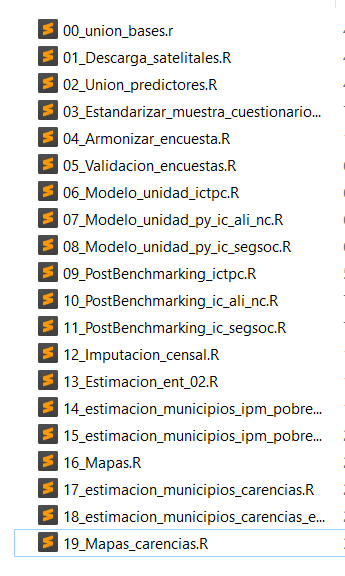
\includegraphics[width=4.16667in,height=\textheight]{recursos/01_Introducción/01_Fig_lista_archivos.png}}
\end{itemize}

\textbf{Cada subcarpeta contiene una serie de scripts organizados secuencialmente, asegurando que el proceso de cálculo y análisis se realice de manera ordenada y reproducible.} Esta estructura facilita la identificación y ejecución de cada paso necesario para obtener los resultados del análisis de pobreza multidimensional.

\begin{itemize}
\item
  \textbf{\texttt{input}}: Esta carpeta contiene dos subcarpetas, una para 2015 y otra para 2020. En cada una de estas encontraremos la base de datos de la ENIGH, la encuesta ampliada del censo para el 2020 o la encuesta intercensal para el 2015, además de las variables predictoras a nivel de municipios. También incluye un archivo en formato CSV que contiene las líneas de pobreza para el año que se esté procesando.
\item
  \textbf{\texttt{output}}: Esta carpeta sigue la misma estructura, con subcarpetas para 2015 y 2020. En cada una de estas subcarpetas encontraremos la carpeta de iteraciones, donde están disponibles los resultados de las iteraciones realizadas por cada estado para cada uno de los municipios. También dispone de una subcarpeta de modelos que contiene los modelos estimados para cada una de las carencias, así como algunos gráficos de validación. Además, encontraremos la carpeta de intermedias necesarias para el procesamiento de información o para el almacenamiento de algunos resultados.
\item
  \textbf{\texttt{shapefile}}: Aquí están disponibles los shapefiles para la realización de mapas y descarga de información satelital, que son utilizados como covariables en la implementación del modelo.
\end{itemize}

Esta organización permite mantener un flujo de trabajo claro y estructurado, donde cada script y conjunto de datos desempeñan un papel específico en el proceso general, desde la preparación de datos hasta la generación de resultados finales.

\hypertarget{librerias-de-r-y-otros-insumos}{%
\subsection*{\texorpdfstring{Librerias de \emph{R} y otros insumos}{Librerias de R y otros insumos}}\label{librerias-de-r-y-otros-insumos}}
\addcontentsline{toc}{subsection}{Librerias de \emph{R} y otros insumos}

En el siguiente apartado, se describe el conjunto de librerías utilizadas para el desarrollo de este proyecto, así como una breve descripción de las bases de datos empleadas.

\hypertarget{libreruxedas-utilizadas}{%
\subsubsection*{Librerías Utilizadas}\label{libreruxedas-utilizadas}}
\addcontentsline{toc}{subsubsection}{Librerías Utilizadas}

\hypertarget{manipulaciuxf3n-y-transformaciuxf3n-de-datos}{%
\paragraph*{Manipulación y Transformación de Datos}\label{manipulaciuxf3n-y-transformaciuxf3n-de-datos}}
\addcontentsline{toc}{paragraph}{Manipulación y Transformación de Datos}

\begin{itemize}
\tightlist
\item
  \textbf{\texttt{tidyverse}}: Conjunto de paquetes (incluyendo \texttt{dplyr}, \texttt{ggplot2}, \texttt{tibble}, \texttt{readr}, \texttt{purrr}, \texttt{tidyr}, y \texttt{stringr}) que facilitan la manipulación y visualización de datos de manera coherente y eficiente.
\item
  \textbf{\texttt{data.table}}: Proporciona herramientas rápidas y eficientes para la manipulación de grandes conjuntos de datos tabulares.
\item
  \textbf{\texttt{dplyr}}: Parte del \texttt{tidyverse}, facilita la manipulación de datos mediante verbos intuitivos como \texttt{select}, \texttt{filter}, \texttt{mutate}, \texttt{summarize}, y \texttt{arrange}.
\item
  \textbf{\texttt{magrittr}}: Introduce el operador \texttt{\%\textgreater{}\%}, permitiendo una escritura de código más clara y encadenada.
\item
  \textbf{\texttt{purrr}}: Extiende las capacidades de programación funcional para trabajar con listas y vectores.
\item
  \textbf{\texttt{furrr}}: Permite realizar operaciones paralelas utilizando \texttt{purrr} y \texttt{future}.
\item
  \textbf{\texttt{stringr}}: Simplifica la manipulación de cadenas de caracteres mediante funciones intuitivas.
\item
  \textbf{\texttt{labelled}}: Facilita la manipulación de datos etiquetados, comúnmente utilizados en encuestas y datos sociológicos.
\end{itemize}

\hypertarget{lectura-y-escritura-de-datos}{%
\paragraph*{Lectura y Escritura de Datos}\label{lectura-y-escritura-de-datos}}
\addcontentsline{toc}{paragraph}{Lectura y Escritura de Datos}

\begin{itemize}
\tightlist
\item
  \textbf{\texttt{openxlsx}}: Permite la creación, lectura y manipulación de archivos Excel sin depender de software adicional.
\item
  \textbf{\texttt{haven}}: Permite leer y escribir datos en formatos usados por otros programas estadísticos como SPSS, Stata y SAS.
\item
  \textbf{\texttt{readstata13}}: Especializado en la lectura de archivos Stata versión 13, asegurando compatibilidad con datos antiguos.
\end{itemize}

\hypertarget{anuxe1lisis-de-datos-de-encuestas}{%
\paragraph*{Análisis de Datos de Encuestas}\label{anuxe1lisis-de-datos-de-encuestas}}
\addcontentsline{toc}{paragraph}{Análisis de Datos de Encuestas}

\begin{itemize}
\tightlist
\item
  \textbf{\texttt{survey}}: Proporciona herramientas para el análisis de datos de encuestas complejas, incluyendo ponderaciones y diseños de muestras.
\item
  \textbf{\texttt{srvyr}}: Ofrece una interfaz más amigable basada en \texttt{dplyr} para trabajar con el paquete \texttt{survey}.
\item
  \textbf{\texttt{TeachingSampling}}: Incluye métodos y herramientas para realizar muestreo en investigaciones educativas.
\item
  \textbf{\texttt{samplesize4surveys}}: Facilita el cálculo del tamaño de muestra necesario para encuestas, asegurando resultados estadísticamente significativos.
\item
  \textbf{\texttt{convey}}: Extiende \texttt{survey} para analizar medidas de desigualdad y pobreza en datos de encuestas.
\end{itemize}

\hypertarget{modelado-y-anuxe1lisis-estaduxedstico}{%
\paragraph*{Modelado y Análisis Estadístico}\label{modelado-y-anuxe1lisis-estaduxedstico}}
\addcontentsline{toc}{paragraph}{Modelado y Análisis Estadístico}

\begin{itemize}
\tightlist
\item
  \textbf{\texttt{rstan}}: Interfaz de R para Stan, que realiza modelado bayesiano avanzado, permitiendo la creación de modelos complejos.
\item
  \textbf{\texttt{lme4}}: Proporciona herramientas para ajustar y analizar modelos lineales y no lineales de efectos mixtos.
\item
  \textbf{\texttt{car}}: Incluye diversas herramientas para la regresión aplicada y diagnósticos de modelos.
\item
  \textbf{\texttt{randomForest}}: Implementa algoritmos de bosque aleatorio para clasificación y regresión.
\item
  \textbf{\texttt{caret}}: Ofrece una amplia gama de herramientas para la creación y validación de modelos de aprendizaje automático.
\item
  \textbf{\texttt{nortest}}: Contiene pruebas para evaluar la normalidad de los datos, esencial en muchos análisis estadísticos.
\end{itemize}

\hypertarget{visualizaciuxf3n-de-datos}{%
\paragraph*{Visualización de Datos}\label{visualizaciuxf3n-de-datos}}
\addcontentsline{toc}{paragraph}{Visualización de Datos}

\begin{itemize}
\tightlist
\item
  \textbf{\texttt{ggplot2}}: Parte del \texttt{tidyverse}, es una potente herramienta para la visualización de datos basada en la gramática de gráficos.
\item
  \textbf{\texttt{DataExplorer}}: Simplifica la exploración inicial y la generación de reportes de datos.
\item
  \textbf{\texttt{thematic}}: Facilita la personalización de temas gráficos en \texttt{ggplot2}, permitiendo una estética consistente.
\item
  \textbf{\texttt{patchwork}}: Permite combinar múltiples gráficos de \texttt{ggplot2} en una única visualización coherente.
\item
  \textbf{\texttt{tmap}}: Especializado en la creación de mapas temáticos, útil para visualizar datos geoespaciales.
\item
  \textbf{\texttt{sf}}: Proporciona una estructura eficiente para manipular datos espaciales, facilitando la integración con \texttt{ggplot2} y \texttt{tmap}.
\end{itemize}

\hypertarget{informes-y-reproducibilidad}{%
\paragraph*{Informes y Reproducibilidad}\label{informes-y-reproducibilidad}}
\addcontentsline{toc}{paragraph}{Informes y Reproducibilidad}

\begin{itemize}
\tightlist
\item
  \textbf{\texttt{printr}}: Mejora el formato de la impresión de resultados en R Markdown, haciendo los informes más legibles.
\item
  \textbf{\texttt{knitr}}: Herramienta clave para la creación de informes dinámicos y reproducibles, integrando código y texto.
\end{itemize}

\hypertarget{integraciuxf3n-con-otros-lenguajes}{%
\paragraph*{Integración con Otros Lenguajes}\label{integraciuxf3n-con-otros-lenguajes}}
\addcontentsline{toc}{paragraph}{Integración con Otros Lenguajes}

\begin{itemize}
\tightlist
\item
  \textbf{\texttt{reticulate}}: Facilita la interoperabilidad entre R y Python, permitiendo ejecutar código de Python dentro de un entorno de R.
\end{itemize}

\hypertarget{bases-de-datos-utilizadas}{%
\subsection*{Bases de Datos Utilizadas}\label{bases-de-datos-utilizadas}}
\addcontentsline{toc}{subsection}{Bases de Datos Utilizadas}

Para este proyecto, se emplearon diversas bases de datos que incluyen:

\begin{itemize}
\tightlist
\item
  \textbf{Encuesta Nacional de Ingresos y Gastos de los Hogares (ENIGH)}: Proporciona información detallada sobre los ingresos y gastos de los hogares en México. Esta encuesta es crucial para entender los patrones de consumo y el bienestar económico de la población.
\item
  \textbf{Formulario Ampliado del Censo 2020}: Ofrece datos sociodemográficos detallados a nivel de hogar y persona. Esta fuente es esencial para capturar una amplia gama de variables necesarias para el análisis multidimensional de la pobreza.
\item
  \textbf{Encuesta Intercensal de 2015}: Complementa la información del censo con datos adicionales recopilados entre periodos censales. Proporciona una actualización intermedia de las condiciones demográficas y socioeconómicas.
\item
  \textbf{Imágenes Satelitales}: Proveen datos geoespaciales esenciales para capturar la diversidad de las condiciones de vida en México. Estas imágenes ayudan a incorporar información espacial detallada en los modelos de estimación.
\end{itemize}

Estas librerías y bases de datos son fundamentales para la implementación de la metodología de estimación del Índice de Pobreza Multidimensional (IPM) y otras carencias en los distintos municipios de México.

\hypertarget{indicadores-estimados}{%
\section*{Indicadores estimados}\label{indicadores-estimados}}
\addcontentsline{toc}{section}{Indicadores estimados}

En esta sección se presentan los diferentes indicadores utilizados para medir y analizar la situación de pobreza y vulnerabilidad en la población. A continuación, se describen los indicadores estimados:
\#\#\# Descripción de las Funciones de Estimación en R

\begin{enumerate}
\def\labelenumi{\arabic{enumi}.}
\tightlist
\item
  \textbf{Población en situación de pobreza multidimensional (I)}

  \begin{itemize}
  \tightlist
  \item
    \textbf{Scripts utilizados}:

    \begin{itemize}
    \tightlist
    \item
      \emph{13\_Estimacion\_ent\_02.R}
    \item
      \emph{14\_estimacion\_municipios\_ipm\_pobreza.R}
    \item
      \emph{15\_estimacion\_municipios\_ipm\_pobreza\_error.R}
    \end{itemize}
  \end{itemize}
\item
  \textbf{Población en situación de pobreza moderada}

  \begin{itemize}
  \tightlist
  \item
    \textbf{Scripts utilizados}:

    \begin{itemize}
    \tightlist
    \item
      \emph{13\_Estimacion\_ent\_02.R}
    \item
      \emph{14\_estimacion\_municipios\_ipm\_pobreza.R}
    \item
      \emph{15\_estimacion\_municipios\_ipm\_pobreza\_error.R}
    \end{itemize}
  \end{itemize}
\item
  \textbf{Población en situación de pobreza extrema}

  \begin{itemize}
  \tightlist
  \item
    \textbf{Scripts utilizados}:

    \begin{itemize}
    \tightlist
    \item
      \emph{13\_Estimacion\_ent\_02.R}
    \item
      \emph{14\_estimacion\_municipios\_ipm\_pobreza.R}
    \item
      \emph{15\_estimacion\_municipios\_ipm\_pobreza\_error.R}
    \end{itemize}
  \end{itemize}
\item
  \textbf{Población vulnerable por carencias sociales (II)}

  \begin{itemize}
  \tightlist
  \item
    \textbf{Scripts utilizados}:

    \begin{itemize}
    \tightlist
    \item
      \emph{13\_Estimacion\_ent\_02.R}
    \item
      \emph{14\_estimacion\_municipios\_ipm\_pobreza.R}
    \item
      \emph{15\_estimacion\_municipios\_ipm\_pobreza\_error.R}
    \end{itemize}
  \end{itemize}
\item
  \textbf{Población vulnerable por ingresos (III)}

  \begin{itemize}
  \tightlist
  \item
    \textbf{Scripts utilizados}:

    \begin{itemize}
    \tightlist
    \item
      \emph{13\_Estimacion\_ent\_02.R}
    \item
      \emph{14\_estimacion\_municipios\_ipm\_pobreza.R}
    \item
      \emph{15\_estimacion\_municipios\_ipm\_pobreza\_error.R}
    \end{itemize}
  \end{itemize}
\item
  \textbf{Población no pobre multidimensional y no vulnerable (IV)}

  \begin{itemize}
  \tightlist
  \item
    \textbf{Scripts utilizados}:

    \begin{itemize}
    \tightlist
    \item
      \emph{13\_Estimacion\_ent\_02.R}
    \item
      \emph{14\_estimacion\_municipios\_ipm\_pobreza.R}
    \item
      \emph{15\_estimacion\_municipios\_ipm\_pobreza\_error.R}
    \end{itemize}
  \end{itemize}
\item
  \textbf{Población con al menos una carencia social (tol\_ic\_1)}

  \begin{itemize}
  \tightlist
  \item
    \textbf{Scripts utilizados}:

    \begin{itemize}
    \tightlist
    \item
      \emph{17\_estimacion\_municipios\_carencias.R}
    \item
      \emph{18\_estimacion\_municipios\_carencias\_error.R}
    \end{itemize}
  \end{itemize}
\item
  \textbf{Población con al menos tres carencias sociales (tol\_ic\_2)}

  \begin{itemize}
  \tightlist
  \item
    \textbf{Scripts utilizados}:

    \begin{itemize}
    \tightlist
    \item
      \emph{17\_estimacion\_municipios\_carencias.R}
    \item
      \emph{18\_estimacion\_municipios\_carencias\_error.R}
    \end{itemize}
  \end{itemize}
\item
  \textbf{Carencia por acceso a la seguridad social (ic\_segsoc)}

  \begin{itemize}
  \tightlist
  \item
    \textbf{Scripts utilizados}:

    \begin{itemize}
    \tightlist
    \item
      \emph{17\_estimacion\_municipios\_carencias.R}
    \item
      \emph{18\_estimacion\_municipios\_carencias\_error.R}
    \end{itemize}
  \end{itemize}
\item
  \textbf{Carencia por acceso a la alimentación nutritiva y de calidad (ic\_ali\_nc)}

  \begin{itemize}
  \tightlist
  \item
    \textbf{Scripts utilizados}:

    \begin{itemize}
    \tightlist
    \item
      \emph{17\_estimacion\_municipios\_carencias.R}
    \item
      \emph{18\_estimacion\_municipios\_carencias\_error.R}
    \end{itemize}
  \end{itemize}
\item
  \textbf{Población con ingreso inferior a la línea de pobreza extrema por ingresos (pobrea\_li)}

  \begin{itemize}
  \tightlist
  \item
    \textbf{Scripts utilizados}:

    \begin{itemize}
    \tightlist
    \item
      \emph{17\_estimacion\_municipios\_carencias.R}
    \item
      \emph{18\_estimacion\_municipios\_carencias\_error.R}
    \end{itemize}
  \end{itemize}
\item
  \textbf{Población con ingreso inferior a la línea de pobreza por ingresos (pobrea\_lp)}

  \begin{itemize}
  \tightlist
  \item
    \textbf{Scripts utilizados}:

    \begin{itemize}
    \tightlist
    \item
      \emph{17\_estimacion\_municipios\_carencias.R}
    \item
      \emph{18\_estimacion\_municipios\_carencias\_error.R}
    \end{itemize}
  \end{itemize}
\item
  \textbf{Rezago educativo}

  \begin{itemize}
  \tightlist
  \item
    \textbf{Script utilizado}:

    \begin{itemize}
    \tightlist
    \item
      \emph{20\_estimacion\_directa\_carencias.R}
    \end{itemize}
  \end{itemize}
\item
  \textbf{Carencia por acceso a los servicios de salud}

  \begin{itemize}
  \tightlist
  \item
    \textbf{Script utilizado}:

    \begin{itemize}
    \tightlist
    \item
      \emph{20\_estimacion\_directa\_carencias.R}
    \end{itemize}
  \end{itemize}
\item
  \textbf{Carencia por calidad y espacios de la vivienda}

  \begin{itemize}
  \tightlist
  \item
    \textbf{Script utilizado}:

    \begin{itemize}
    \tightlist
    \item
      \emph{20\_estimacion\_directa\_carencias.R}
    \end{itemize}
  \end{itemize}
\item
  \textbf{Carencia por acceso a los servicios básicos en la vivienda}

  \begin{itemize}
  \tightlist
  \item
    \textbf{Script utilizado}:

    \begin{itemize}
    \tightlist
    \item
      \emph{20\_estimacion\_directa\_carencias.R}
    \end{itemize}
  \end{itemize}
\end{enumerate}

\hypertarget{union_bases.r}{%
\chapter*{00\_union\_bases.R}\label{union_bases.r}}
\addcontentsline{toc}{chapter}{00\_union\_bases.R}

Para la ejecución del presente archivo, debe abrir el archivo \textbf{00\_union\_bases.R} disponible en la ruta \emph{Rcodes/2020/00\_union\_bases.R}.

El código comienza limpiando el entorno de R y cargando varias bibliotecas esenciales para la manipulación y análisis de datos. Posteriormente, define un conjunto de variables a validar y obtiene listas de archivos de datos en formato \texttt{.dta} correspondientes a diferentes conjuntos de datos del censo 2020. A continuación, el código itera sobre estos archivos para leer, combinar y almacenar los datos de cada estado en archivos \texttt{.rds} individuales. Estos datos se combinan en un único dataframe que se guarda para su uso posterior.

En la sección final, el código se centra en los datos de la ENIGH 2020. Lee los archivos de hogares y pobreza, y los combina utilizando un \texttt{inner\_join}. Se seleccionan y renombran variables clave para asegurar la consistencia en el análisis. Finalmente, el dataframe combinado se guarda en un archivo \texttt{.rds} para facilitar el acceso y análisis futuros.

\hypertarget{limpieza-del-entorno-y-carga-de-bibliotecas}{%
\subsubsection*{Limpieza del Entorno y Carga de Bibliotecas}\label{limpieza-del-entorno-y-carga-de-bibliotecas}}
\addcontentsline{toc}{subsubsection}{Limpieza del Entorno y Carga de Bibliotecas}

Se limpia el entorno de R eliminando todos los objetos y se ejecuta el recolector de basura para liberar memoria.

\begin{Shaded}
\begin{Highlighting}[]
\FunctionTok{rm}\NormalTok{(}\AttributeTok{list =} \FunctionTok{ls}\NormalTok{())}
\FunctionTok{gc}\NormalTok{()}
\end{Highlighting}
\end{Shaded}

Se cargan varias bibliotecas esenciales para la manipulación y análisis de datos, incluyendo \texttt{tidyverse}, \texttt{data.table}, \texttt{haven} y otras.

\begin{Shaded}
\begin{Highlighting}[]
\FunctionTok{library}\NormalTok{(tidyverse)}
\FunctionTok{library}\NormalTok{(data.table)}
\FunctionTok{library}\NormalTok{(openxlsx)}
\FunctionTok{library}\NormalTok{(magrittr)}
\FunctionTok{library}\NormalTok{(DataExplorer)}
\FunctionTok{library}\NormalTok{(haven)}
\FunctionTok{library}\NormalTok{(purrr)}
\FunctionTok{library}\NormalTok{(furrr)}
\FunctionTok{library}\NormalTok{(labelled)}
\FunctionTok{cat}\NormalTok{(}\StringTok{"}\SpecialCharTok{\textbackslash{}f}\StringTok{"}\NormalTok{)}
\end{Highlighting}
\end{Shaded}

\hypertarget{configuraciuxf3n-de-la-memoria}{%
\subsubsection*{Configuración de la Memoria}\label{configuraciuxf3n-de-la-memoria}}
\addcontentsline{toc}{subsubsection}{Configuración de la Memoria}

Se define un límite para la memoria RAM a utilizar, en este caso 250 GB.

\begin{Shaded}
\begin{Highlighting}[]
\FunctionTok{memory.limit}\NormalTok{(}\DecValTok{250000000}\NormalTok{)}
\end{Highlighting}
\end{Shaded}

\hypertarget{definiciuxf3n-de-variables-y-obtenciuxf3n-de-archivos}{%
\subsubsection*{Definición de Variables y Obtención de Archivos}\label{definiciuxf3n-de-variables-y-obtenciuxf3n-de-archivos}}
\addcontentsline{toc}{subsubsection}{Definición de Variables y Obtención de Archivos}

Para llevar a cabo la validación y procesamiento de datos del censo 2020, se define un conjunto de variables que serán validadas. Estas variables incluyen indicadores clave como rezago educativo (\texttt{ic\_rezedu}), acceso a servicios de salud (\texttt{ic\_asalud}), seguridad social (\texttt{ic\_segsoc}), calidad de la vivienda (\texttt{ic\_cv}), servicios básicos en la vivienda (\texttt{ic\_sbv}), acceso a alimentación nutritiva y de calidad (\texttt{ic\_ali\_nc}), y el índice de pobreza multidimensional (\texttt{ictpc}).

\begin{Shaded}
\begin{Highlighting}[]
\NormalTok{validar\_var }\OtherTok{\textless{}{-}} \FunctionTok{c}\NormalTok{(}
  \StringTok{"ic\_rezedu"}\NormalTok{,}
  \StringTok{"ic\_asalud"}\NormalTok{,}
  \StringTok{"ic\_segsoc"}\NormalTok{,}
  \StringTok{"ic\_cv"}\NormalTok{,}
  \StringTok{"ic\_sbv"}\NormalTok{,}
  \StringTok{"ic\_ali\_nc"}\NormalTok{,}
  \StringTok{"ictpc"}
\NormalTok{)}
\end{Highlighting}
\end{Shaded}

Posteriormente, se obtienen listas de archivos con extensión \texttt{.dta}, que corresponden a diferentes conjuntos de datos del censo 2020. Estos archivos se organizan en tres categorías principales:

\begin{enumerate}
\def\labelenumi{\arabic{enumi}.}
\tightlist
\item
  \textbf{Archivos de muestra del censo 2020 por estado}: Se buscan archivos en la ruta \texttt{../input/2020/muestra\_ampliada/SegSocial/SegSoc/} que contengan información de seguridad social.
\end{enumerate}

\begin{Shaded}
\begin{Highlighting}[]
\NormalTok{file\_muestra\_censo\_2020\_estado }\OtherTok{\textless{}{-}} \FunctionTok{list.files}\NormalTok{(}
  \StringTok{"../input/2020/muestra\_ampliada/SegSocial/SegSoc/"}\NormalTok{,}
  \AttributeTok{full.names =} \ConstantTok{TRUE}\NormalTok{,}
  \AttributeTok{pattern =} \StringTok{"dta$"}
\NormalTok{)}
\end{Highlighting}
\end{Shaded}

\begin{enumerate}
\def\labelenumi{\arabic{enumi}.}
\setcounter{enumi}{1}
\tightlist
\item
  \textbf{Archivos complementarios de muestra del censo 2020 por estado}: Se buscan archivos adicionales en la ruta
  \texttt{../input/2020/muestra\_ampliada/SegSocial/Complemento\_SegSoc/} que contienen datos complementarios de seguridad social.
\end{enumerate}

\begin{Shaded}
\begin{Highlighting}[]
\NormalTok{file\_muestra\_censo\_2020\_estado\_complemento }\OtherTok{\textless{}{-}} \FunctionTok{list.files}\NormalTok{(}
  \StringTok{"../input/2020/muestra\_ampliada/SegSocial/Complemento\_SegSoc/"}\NormalTok{,}
  \AttributeTok{full.names =} \ConstantTok{TRUE}\NormalTok{,}
  \AttributeTok{pattern =} \StringTok{"dta$"}
\NormalTok{)}
\end{Highlighting}
\end{Shaded}

\begin{enumerate}
\def\labelenumi{\arabic{enumi}.}
\setcounter{enumi}{2}
\tightlist
\item
  \textbf{Archivos de cuestionario ampliado del censo 2020 por estado}: Se buscan archivos en la ruta \texttt{../input/2020/muestra\_ampliada/IndicadoresCenso/} que incluyen indicadores generales del censo.
\end{enumerate}

\begin{Shaded}
\begin{Highlighting}[]
\NormalTok{muestra\_cuestionario\_ampliado\_censo\_2020\_estado }\OtherTok{\textless{}{-}} \FunctionTok{list.files}\NormalTok{(}
  \StringTok{"../input/2020/muestra\_ampliada/IndicadoresCenso/"}\NormalTok{,}
  \AttributeTok{full.names =} \ConstantTok{TRUE}\NormalTok{,}
  \AttributeTok{pattern =} \StringTok{"dta$"}
\NormalTok{)}
\end{Highlighting}
\end{Shaded}

Estas listas de archivos permiten acceder y gestionar de manera eficiente los datos necesarios para el análisis y validación de los indicadores de pobreza y carencias sociales del censo 2020.

\hypertarget{lectura-y-combinaciuxf3n-de-datos-del-censo}{%
\subsubsection*{Lectura y Combinación de Datos del Censo}\label{lectura-y-combinaciuxf3n-de-datos-del-censo}}
\addcontentsline{toc}{subsubsection}{Lectura y Combinación de Datos del Censo}

Este bloque de código está diseñado para leer, combinar y guardar datos provenientes de múltiples archivos del censo. El objetivo es consolidar la información de diferentes fuentes en un único dataframe y almacenar los resultados intermedios y finales en archivos \texttt{.rds}.

\begin{Shaded}
\begin{Highlighting}[]
\NormalTok{df }\OtherTok{\textless{}{-}} \FunctionTok{data.frame}\NormalTok{()}

\ControlFlowTok{for}\NormalTok{ (ii }\ControlFlowTok{in} \DecValTok{1}\SpecialCharTok{:}\DecValTok{32}\NormalTok{) \{}
\NormalTok{  muestra\_censo\_2020\_estado\_ii }\OtherTok{\textless{}{-}}
    \FunctionTok{read\_dta}\NormalTok{(file\_muestra\_censo\_2020\_estado[ii])}
\NormalTok{  muestra\_censo\_2020\_estado\_complemento\_ii }\OtherTok{\textless{}{-}}
    \FunctionTok{read\_dta}\NormalTok{(file\_muestra\_censo\_2020\_estado\_complemento[ii]) }\SpecialCharTok{\%\textgreater{}\%}
    \FunctionTok{mutate}\NormalTok{(}\AttributeTok{id\_per =}\NormalTok{ id\_persona)}
\NormalTok{  muestra\_cuestionario\_ampliado\_censo\_2020\_estado\_ii }\OtherTok{\textless{}{-}}
    \FunctionTok{read\_dta}\NormalTok{(muestra\_cuestionario\_ampliado\_censo\_2020\_estado[ii])}
  
\NormalTok{  muestra\_censo }\OtherTok{\textless{}{-}}
    \FunctionTok{inner\_join}\NormalTok{(muestra\_censo\_2020\_estado\_ii,}
\NormalTok{               muestra\_censo\_2020\_estado\_complemento\_ii) }\SpecialCharTok{\%\textgreater{}\%}
    \FunctionTok{select}\NormalTok{(}\SpecialCharTok{{-}}\NormalTok{tamloc) }\SpecialCharTok{\%\textgreater{}\%}
    \FunctionTok{inner\_join}\NormalTok{(muestra\_cuestionario\_ampliado\_censo\_2020\_estado\_ii)}
  
  \FunctionTok{saveRDS}\NormalTok{(muestra\_censo,}
          \FunctionTok{paste0}\NormalTok{(}\StringTok{"../output/2020/muestra\_censo/depto\_"}\NormalTok{, ii, }\StringTok{".rds"}\NormalTok{))}
  
\NormalTok{  df }\OtherTok{\textless{}{-}} \FunctionTok{bind\_rows}\NormalTok{(df, muestra\_censo)}
  \FunctionTok{cat}\NormalTok{(file\_muestra\_censo\_2020\_estado[ii], }\StringTok{"}\SpecialCharTok{\textbackslash{}n}\StringTok{"}\NormalTok{)}
\NormalTok{\}}
\end{Highlighting}
\end{Shaded}

Se guarda el dataframe combinado en un archivo \texttt{.rds}.

\begin{Shaded}
\begin{Highlighting}[]
\FunctionTok{saveRDS}\NormalTok{(df, }\AttributeTok{file =} \StringTok{"../output/2020/muestra\_cuestionario\_ampliado.rds"}\NormalTok{)}
\end{Highlighting}
\end{Shaded}

\hypertarget{lectura-y-combinaciuxf3n-de-datos-de-la-enigh}{%
\subsubsection*{Lectura y Combinación de Datos de la ENIGH}\label{lectura-y-combinaciuxf3n-de-datos-de-la-enigh}}
\addcontentsline{toc}{subsubsection}{Lectura y Combinación de Datos de la ENIGH}

Este bloque de código está diseñado para leer, verificar y combinar datos de la Encuesta Nacional de Ingresos y Gastos de los Hogares (ENIGH) 2020. La finalidad es consolidar la información de diferentes archivos de datos en un único dataframe para su posterior análisis.

\begin{Shaded}
\begin{Highlighting}[]
\NormalTok{enigh\_hogares }\OtherTok{\textless{}{-}} \FunctionTok{read\_dta}\NormalTok{(}\StringTok{"../input/2020/enigh/base\_hogares20.dta"}\NormalTok{)}
\NormalTok{enigh\_pobreza }\OtherTok{\textless{}{-}} \FunctionTok{read\_dta}\NormalTok{(}\StringTok{"../input/2020/enigh/pobreza\_20.dta"}\NormalTok{) }\SpecialCharTok{\%\textgreater{}\%} 
  \FunctionTok{select}\NormalTok{(}\SpecialCharTok{{-}}\NormalTok{ent)}
\end{Highlighting}
\end{Shaded}

Se leen los datos de hogares y pobreza de la ENIGH 2020.

\begin{Shaded}
\begin{Highlighting}[]
\FunctionTok{n\_distinct}\NormalTok{(enigh\_pobreza}\SpecialCharTok{$}\NormalTok{folioviv)}
\FunctionTok{n\_distinct}\NormalTok{(enigh\_hogares}\SpecialCharTok{$}\NormalTok{folioviv)}
\end{Highlighting}
\end{Shaded}

Se verifica la unicidad de los identificadores de viviendas.

\begin{Shaded}
\begin{Highlighting}[]
\NormalTok{enigh }\OtherTok{\textless{}{-}} \FunctionTok{inner\_join}\NormalTok{(}
\NormalTok{  enigh\_pobreza,}
\NormalTok{  enigh\_hogares,}
  \AttributeTok{by =} \FunctionTok{join\_by}\NormalTok{(}
\NormalTok{    folioviv, foliohog, est\_dis, upm,}
\NormalTok{    factor, rururb, ubica\_geo}
\NormalTok{  ), }
  \AttributeTok{suffix =} \FunctionTok{c}\NormalTok{(}\StringTok{"\_pers"}\NormalTok{, }\StringTok{"\_hog"}\NormalTok{)}
\NormalTok{)}
\end{Highlighting}
\end{Shaded}

Se combinan los datos de pobreza y hogares utilizando un \texttt{inner\_join}.

\hypertarget{selecciuxf3n-y-renombramiento-de-variables}{%
\subsubsection*{Selección y Renombramiento de Variables}\label{selecciuxf3n-y-renombramiento-de-variables}}
\addcontentsline{toc}{subsubsection}{Selección y Renombramiento de Variables}

En esta sección, se seleccionan y renombran algunas variables clave del dataframe combinado para asegurar la consistencia en el análisis y facilitar su manipulación posterior.

\begin{Shaded}
\begin{Highlighting}[]
\NormalTok{   enigh}\SpecialCharTok{$}\NormalTok{ic\_ali\_nc}
\NormalTok{   enigh}\SpecialCharTok{$}\NormalTok{ictpc\_pers}
\NormalTok{   enigh}\SpecialCharTok{$}\NormalTok{ictpc }\OtherTok{\textless{}{-}}\NormalTok{ enigh}\SpecialCharTok{$}\NormalTok{ictpc\_pers}
\NormalTok{   enigh}\SpecialCharTok{$}\NormalTok{ic\_segsoc}
\end{Highlighting}
\end{Shaded}

\begin{itemize}
\tightlist
\item
  \texttt{enigh\$ic\_ali\_nc}: Selección de la variable que indica carencia por acceso a la alimentación nutritiva y de calidad.
\item
  \texttt{enigh\$ictpc\_pers}: Selección de la variable que representa el ingreso corriente total por persona.
\item
  \texttt{enigh\$ictpc\ \textless{}-\ enigh\$ictpc\_pers}: Renombramiento de \texttt{ictpc\_pers} a \texttt{ictpc} para simplificar su uso en análisis posteriores.
\item
  \texttt{enigh\$ic\_segsoc}: Selección de la variable que indica carencia por acceso a la seguridad social.
\end{itemize}

\hypertarget{guardado-del-dataframe-combinado}{%
\subsubsection*{Guardado del DataFrame Combinado}\label{guardado-del-dataframe-combinado}}
\addcontentsline{toc}{subsubsection}{Guardado del DataFrame Combinado}

Finalmente, se guarda el dataframe combinado en un archivo \texttt{.rds} para facilitar el acceso y análisis futuros.

\begin{Shaded}
\begin{Highlighting}[]
   \FunctionTok{saveRDS}\NormalTok{(enigh, }\AttributeTok{file =} \StringTok{"../output/2020/enigh.rds"}\NormalTok{)}
\end{Highlighting}
\end{Shaded}

Se guarda el dataframe \texttt{enigh} en un archivo \texttt{.rds} en la ruta especificada \texttt{../output/2020/enigh.rds}.

\hypertarget{descarga_satelitales.r}{%
\chapter*{01\_Descarga\_satelitales.R}\label{descarga_satelitales.r}}
\addcontentsline{toc}{chapter}{01\_Descarga\_satelitales.R}

Para la ejecución del presente archivo, debe abrir el archivo \textbf{01\_Descarga\_satelitales.R} disponible en la ruta \emph{Rcodes/2020/01\_Descarga\_satelitales.R}.

Este código en R se enfoca en el procesamiento y análisis de datos geoespaciales utilizando una combinación de bibliotecas y herramientas de Google Earth Engine. La primera parte del script configura el entorno de trabajo, carga las librerías necesarias, y establece la conexión con Python mediante la biblioteca \texttt{reticulate}, esencial para trabajar con \texttt{rgee}, que es la interfaz de R para Google Earth Engine.

En la segunda parte, se realiza la limpieza y transformación de datos espaciales. Se cargan y transforman archivos shapefiles de México a un sistema de referencia de coordenadas adecuado y se convierten a un formato \texttt{MULTIPOLYGON}. Luego, se extraen y procesan datos de imágenes satelitales para diversas variables como luminosidad, urbanización, y distancia a servicios de salud utilizando colecciones de imágenes de Google Earth Engine. Estos datos se agrupan por región y se guardan en archivos RDS para su análisis posterior. Finalmente, se combinan todos los datos procesados en un único dataframe y se escalan para prepararlos para su uso en modelos o análisis adicionales.

\hypertarget{lectura-de-libreruxedas}{%
\subsubsection*{Lectura de Librerías}\label{lectura-de-libreruxedas}}
\addcontentsline{toc}{subsubsection}{Lectura de Librerías}

Para comenzar, se realiza una limpieza del entorno de trabajo en R mediante la eliminación de todos los objetos existentes usando \texttt{rm(list\ =\ ls())}. Esto asegura que no haya interferencias de sesiones anteriores y que el entorno esté limpio. Luego, se establece un límite de memoria de 500,000 MB con \texttt{memory.limit(500000)}, lo que permite manejar grandes volúmenes de datos sin que R se quede sin memoria, preparando el entorno para análisis intensivos.

A continuación, se cargan varias librerías esenciales para el análisis de datos. \texttt{tidyverse} se utiliza para la manipulación y visualización de datos de manera eficiente, mientras que \texttt{sampling} proporciona herramientas para realizar muestreo estadístico. \texttt{rgee} permite la conexión con Google Earth Engine para realizar análisis geoespaciales avanzados. \texttt{sf} es fundamental para manejar datos geográficos, y \texttt{concaveman} ayuda a generar polígonos cóncavos a partir de conjuntos de puntos. Además, \texttt{geojsonio} facilita la conversión entre diversos formatos de datos geoespaciales, \texttt{magrittr} mejora la legibilidad del código con el operador \texttt{\%\textgreater{}\%}, \texttt{furrr} habilita la programación paralela utilizando \texttt{purrr}, y \texttt{readr} se emplea para la lectura eficiente de archivos de datos en formatos como CSV.

\begin{Shaded}
\begin{Highlighting}[]
\FunctionTok{rm}\NormalTok{(}\AttributeTok{list =} \FunctionTok{ls}\NormalTok{())}

\FunctionTok{memory.limit}\NormalTok{(}\DecValTok{500000}\NormalTok{)}

\FunctionTok{library}\NormalTok{(tidyverse)}
\FunctionTok{library}\NormalTok{(sampling)}
\FunctionTok{library}\NormalTok{(rgee) }\CommentTok{\# Conexión con Google Earth Engine}
\FunctionTok{library}\NormalTok{(sf) }\CommentTok{\# Paquete para manejar datos geográficos}
\FunctionTok{library}\NormalTok{(concaveman)}
\FunctionTok{library}\NormalTok{(geojsonio)}
\FunctionTok{library}\NormalTok{(magrittr)}
\FunctionTok{library}\NormalTok{(furrr)}
\FunctionTok{library}\NormalTok{(readr)}
\end{Highlighting}
\end{Shaded}

\hypertarget{configuraciuxf3n-inicial-de-python}{%
\subsubsection*{configuración inicial de Python}\label{configuraciuxf3n-inicial-de-python}}
\addcontentsline{toc}{subsubsection}{configuración inicial de Python}

Para comenzar, se obtiene la lista de entornos conda disponibles y se selecciona el entorno llamado ``rgee\_py'', que es específico para la conexión con Google Earth Engine mediante \texttt{rgee}. Esto asegura que se utilice el entorno de Python correcto para las operaciones geoespaciales.

Luego, se configura \texttt{reticulate} para usar el entorno de Python especificado. La función \texttt{py\_config()} verifica la configuración de Python y se carga la librería \texttt{reticulate} para habilitar la conexión entre R y Python, lo que permite ejecutar código Python directamente desde R.

Finalmente, se establece el entorno de Python para \texttt{rgee} mediante \texttt{ee\_install\_set\_pyenv()}, y se configuran las variables de entorno para asegurar que \texttt{reticulate} y \texttt{rgee} usen el entorno de Python correcto. La función \texttt{ee\_Initialize(drive\ =\ T)} inicializa la conexión con Google Earth Engine, permitiendo el acceso y manipulación de datos geoespaciales desde R.

\begin{Shaded}
\begin{Highlighting}[]
\NormalTok{rgee\_environment\_dir }\OtherTok{\textless{}{-}}\NormalTok{ reticulate}\SpecialCharTok{::}\FunctionTok{conda\_list}\NormalTok{()}
\NormalTok{rgee\_environment\_dir }\OtherTok{\textless{}{-}}
\NormalTok{  rgee\_environment\_dir[rgee\_environment\_dir}\SpecialCharTok{$}\NormalTok{name }\SpecialCharTok{==} \StringTok{"rgee\_py"}\NormalTok{, }\DecValTok{2}\NormalTok{]}
\NormalTok{reticulate}\SpecialCharTok{::}\FunctionTok{use\_python}\NormalTok{(rgee\_environment\_dir, }\AttributeTok{required =}\NormalTok{ T)}
\NormalTok{reticulate}\SpecialCharTok{::}\FunctionTok{py\_config}\NormalTok{()}
\FunctionTok{library}\NormalTok{(reticulate) }\CommentTok{\# Conexión con Python}

\NormalTok{rgee}\SpecialCharTok{::}\FunctionTok{ee\_install\_set\_pyenv}\NormalTok{(}\AttributeTok{py\_path =}\NormalTok{ rgee\_environment\_dir, }\AttributeTok{py\_env =} \StringTok{"rgee\_py"}\NormalTok{)}
\FunctionTok{Sys.setenv}\NormalTok{(}\AttributeTok{RETICULATE\_PYTHON =}\NormalTok{ rgee\_environment\_dir)}
\FunctionTok{Sys.setenv}\NormalTok{(}\AttributeTok{EARTHENGINE\_PYTHON =}\NormalTok{ rgee\_environment\_dir)}
\NormalTok{rgee}\SpecialCharTok{::}\FunctionTok{ee\_Initialize}\NormalTok{(}\AttributeTok{drive =}\NormalTok{ T)}
\end{Highlighting}
\end{Shaded}

\hypertarget{arreglar-la-shapefile}{%
\subsubsection*{Arreglar la shapefile}\label{arreglar-la-shapefile}}
\addcontentsline{toc}{subsubsection}{Arreglar la shapefile}

Este bloque de código está diseñado para procesar y transformar archivos shapefile (archivos de formato geoespacial) de México para asegurarse de que estén en el formato correcto y preparados para su análisis. Incluye la lectura de archivos, la transformación del sistema de referencia de coordenadas (CRS), la combinación de los archivos shapefile y la corrección de la codificación de caracteres.

Primero, se descomenta la configuración para ejecutar en paralelo con dos trabajadores usando \texttt{plan(multisession,\ workers\ =\ 2)}, lo que mejora la eficiencia del procesamiento. Luego, se listan los archivos shapefile en el directorio ``shapefile/2020/'' y se leen en una lista \texttt{MEX} utilizando \texttt{furrr::future\_map()}, que permite el procesamiento en paralelo. Cada archivo se transforma para seleccionar columnas específicas (CVEGEO, NOM\_ENT, NOMGEO, y geometry). La función \texttt{st\_transform()} se utiliza para cambiar el sistema de referencia de coordenadas a WGS84, y \texttt{st\_cast()} convierte los objetos geométricos a ``MULTIPOLYGON''.

Después de la transformación y combinación, se unen todos los shapefiles en un solo objeto usando \texttt{bind\_rows()}. Para asegurar que los nombres geográficos estén en la codificación correcta, se usa \texttt{iconv()} para convertir \texttt{NOMGEO} a UTF-8 desde ISO-8859-1. El archivo shapefile transformado y combinado se guarda con \texttt{st\_write()} en la ubicación ``shapefile/2020/MEX\_2020.shp''.

Finalmente, se limpia el entorno con \texttt{rm(list\ =\ ls())}, y el archivo shapefile resultante se lee nuevamente con \texttt{read\_sf()}. Se agrega una nueva columna \texttt{ent} mediante \texttt{mutate()} para extraer los dos primeros caracteres de \texttt{CVEGEO}, que representan la entidad federativa.

\begin{Shaded}
\begin{Highlighting}[]
\CommentTok{\# plan(multisession, workers = 2)}
\CommentTok{\# }
\CommentTok{\# MEX \textless{}{-} list.files("shapefile/2020/", pattern = "shp$",}
\CommentTok{\#            full.names = TRUE) \%\textgreater{}\%}
\CommentTok{\#   furrr::future\_map(\textasciitilde{}read\_sf(.x) \%\textgreater{}\%}
\CommentTok{\#                           select(CVEGEO, NOM\_ENT, NOMGEO,geometry),}
\CommentTok{\#                     .progress = TRUE)}
\CommentTok{\# }
\CommentTok{\# mi\_crs \textless{}{-} "+proj=longlat +datum=WGS84"}
\CommentTok{\# }
\CommentTok{\# \# Transforma el polígono al nuevo CRS}
\CommentTok{\# MEX\_trans \textless{}{-} map(MEX,  \textasciitilde{}st\_transform(.x, crs = mi\_crs))}
\CommentTok{\# MEX\_trans \textless{}{-} map(MEX\_trans,  \textasciitilde{}st\_cast(.x, "MULTIPOLYGON"))}
\CommentTok{\# }
\CommentTok{\# MEX\_trans \textless{}{-} bind\_rows(MEX\_trans)}
\CommentTok{\# }
\CommentTok{\# }
\CommentTok{\# \# stringi::stri\_enc\_detect(MEX\_trans$NOMGEO)}
\CommentTok{\# }
\CommentTok{\# MEX\_trans$NOMGEO \textless{}{-} iconv(MEX\_trans$NOMGEO,}
\CommentTok{\#                           to = "UTF{-}8", from = "ISO{-}8859{-}1")}
\CommentTok{\# }
\CommentTok{\# }
\CommentTok{\# st\_write(MEX\_trans,}
\CommentTok{\#          "shapefile/2020/MEX\_2020.shp",}
\CommentTok{\#          append = TRUE)}
\CommentTok{\# }
\CommentTok{\# rm(list = ls())}

\NormalTok{MEX }\OtherTok{\textless{}{-}} \FunctionTok{read\_sf}\NormalTok{(}\StringTok{"../shapefile/2020/MEX\_2020.shp"}\NormalTok{)}

\NormalTok{MEX }\SpecialCharTok{\%\textless{}\textgreater{}\%} \FunctionTok{mutate}\NormalTok{(}\AttributeTok{ent =} \FunctionTok{substr}\NormalTok{(CVEGEO,}\DecValTok{1}\NormalTok{,}\DecValTok{2}\NormalTok{))}
\end{Highlighting}
\end{Shaded}

\hypertarget{descargar-las-imegenes-satelitales}{%
\subsubsection*{Descargar las imegenes satelitales}\label{descargar-las-imegenes-satelitales}}
\addcontentsline{toc}{subsubsection}{Descargar las imegenes satelitales}

Este bloque de código se centra en la descarga y procesamiento de imágenes satelitales utilizando Google Earth Engine (GEE) en R. Se recopilan datos de diferentes fuentes satelitales para diversas características geoespaciales de México, incluyendo luces nocturnas, cobertura urbana y agrícola, accesibilidad a servicios de salud y modificación humana global. Cada conjunto de datos se extrae, procesa y guarda para su uso posterior en análisis.

\hypertarget{luces-nocturnas}{%
\paragraph*{Luces Nocturnas}\label{luces-nocturnas}}
\addcontentsline{toc}{paragraph}{Luces Nocturnas}

Se utiliza la colección de imágenes ``NOAA/VIIRS/DNB/ANNUAL\_V21'' para obtener datos de luces nocturnas del año 2020. Las imágenes se filtran por fecha y se selecciona la banda ``average''. Posteriormente, se extraen los datos de luces nocturnas promedio para cada entidad federativa en México, y se combinan los resultados en un solo dataframe. Finalmente, se guardan los datos en un archivo \texttt{.rds}.

\begin{Shaded}
\begin{Highlighting}[]
\CommentTok{\#https://developers.google.com/earth{-}engine/datasets/catalog/NOAA\_VIIRS\_DNB\_ANNUAL\_V21\#bands}

\NormalTok{luces }\OtherTok{=}\NormalTok{ ee}\SpecialCharTok{$}\FunctionTok{ImageCollection}\NormalTok{(}\StringTok{"NOAA/VIIRS/DNB/ANNUAL\_V21"}\NormalTok{) }\SpecialCharTok{\%\textgreater{}\%}
\NormalTok{  ee}\SpecialCharTok{$}\NormalTok{ImageCollection}\SpecialCharTok{$}\FunctionTok{filterDate}\NormalTok{(}\StringTok{"2020{-}01{-}01"}\NormalTok{, }\StringTok{"2021{-}01{-}01"}\NormalTok{) }\SpecialCharTok{\%\textgreater{}\%}
\NormalTok{  ee}\SpecialCharTok{$}\NormalTok{ImageCollection}\SpecialCharTok{$}\FunctionTok{map}\NormalTok{(}\ControlFlowTok{function}\NormalTok{(x) x}\SpecialCharTok{$}\FunctionTok{select}\NormalTok{(}\StringTok{"average"}\NormalTok{)) }\SpecialCharTok{\%\textgreater{}\%}
\NormalTok{  ee}\SpecialCharTok{$}\NormalTok{ImageCollection}\SpecialCharTok{$}\FunctionTok{toBands}\NormalTok{()}
\FunctionTok{ee\_print}\NormalTok{(luces)}

\NormalTok{MEX\_luces }\OtherTok{\textless{}{-}} \FunctionTok{map}\NormalTok{(}\FunctionTok{unique}\NormalTok{(MEX}\SpecialCharTok{$}\NormalTok{ent),}
                 \SpecialCharTok{\textasciitilde{}}\FunctionTok{tryCatch}\NormalTok{(}\FunctionTok{ee\_extract}\NormalTok{(}
                   \AttributeTok{x =}\NormalTok{ luces,}
                   \AttributeTok{y =}\NormalTok{ MEX[}\FunctionTok{c}\NormalTok{(}\StringTok{"ent"}\NormalTok{,}\StringTok{"CVEGEO"}\NormalTok{)] }\SpecialCharTok{\%\textgreater{}\%}
                     \FunctionTok{filter}\NormalTok{(ent }\SpecialCharTok{==}\NormalTok{ .x),}
\NormalTok{                   ee}\SpecialCharTok{$}\NormalTok{Reducer}\SpecialCharTok{$}\FunctionTok{mean}\NormalTok{(),}
                   \AttributeTok{sf =} \ConstantTok{FALSE}
\NormalTok{                 ) , }
                 \AttributeTok{error =} \ControlFlowTok{function}\NormalTok{(e)}\FunctionTok{data.frame}\NormalTok{(}\AttributeTok{ent =}\NormalTok{ .x)) }
\NormalTok{)}


\NormalTok{MEX\_luces }\SpecialCharTok{\%\textless{}\textgreater{}\%} \FunctionTok{bind\_rows}\NormalTok{()}

\NormalTok{MEX\_luces }\SpecialCharTok{\%\textgreater{}\%} \FunctionTok{filter}\NormalTok{(}\FunctionTok{is.na}\NormalTok{(X20200101\_average)) }\SpecialCharTok{\%\textgreater{}\%} \FunctionTok{select}\NormalTok{(CVEGEO) }


\FunctionTok{saveRDS}\NormalTok{(MEX\_luces, }\StringTok{"../output/2020/Satelital/MEX\_luces.rds"}\NormalTok{)}
\end{Highlighting}
\end{Shaded}

\hypertarget{urbanismo-y-cultivos}{%
\paragraph*{Urbanismo y Cultivos}\label{urbanismo-y-cultivos}}
\addcontentsline{toc}{paragraph}{Urbanismo y Cultivos}

Se extraen datos de cobertura urbana y de cultivos de la colección ``COPERNICUS/Landcover/100m/Proba-V-C3/Global'' para el año 2019. Se seleccionan las bandas ``urban-coverfraction'' y ``crops-coverfraction'', y se calculan los promedios de estas coberturas para cada entidad federativa. Los resultados se combinan y se guardan en un archivo \texttt{.rds}.

\begin{Shaded}
\begin{Highlighting}[]
\NormalTok{tiposuelo }\OtherTok{=}\NormalTok{ ee}\SpecialCharTok{$}\FunctionTok{ImageCollection}\NormalTok{(}\StringTok{"COPERNICUS/Landcover/100m/Proba{-}V{-}C3/Global"}\NormalTok{) }\SpecialCharTok{\%\textgreater{}\%}
\NormalTok{  ee}\SpecialCharTok{$}\NormalTok{ImageCollection}\SpecialCharTok{$}\FunctionTok{filterDate}\NormalTok{(}\StringTok{"2019{-}01{-}01"}\NormalTok{, }\StringTok{"2019{-}12{-}31"}\NormalTok{) }\SpecialCharTok{\%\textgreater{}\%}
\NormalTok{  ee}\SpecialCharTok{$}\NormalTok{ImageCollection}\SpecialCharTok{$}\FunctionTok{map}\NormalTok{(}\ControlFlowTok{function}\NormalTok{(x)}
\NormalTok{    x}\SpecialCharTok{$}\FunctionTok{select}\NormalTok{(}\StringTok{"urban{-}coverfraction"}\NormalTok{, }\StringTok{"crops{-}coverfraction"}\NormalTok{)) }\SpecialCharTok{\%\textgreater{}\%}
\NormalTok{  ee}\SpecialCharTok{$}\NormalTok{ImageCollection}\SpecialCharTok{$}\FunctionTok{toBands}\NormalTok{()}
\FunctionTok{ee\_print}\NormalTok{(tiposuelo)}

\NormalTok{MEX\_urbano\_cultivo }\OtherTok{\textless{}{-}} \FunctionTok{map}\NormalTok{(}\FunctionTok{unique}\NormalTok{(MEX}\SpecialCharTok{$}\NormalTok{CVEGEO),}
                          \SpecialCharTok{\textasciitilde{}}\FunctionTok{tryCatch}\NormalTok{(}\FunctionTok{ee\_extract}\NormalTok{(}
                            \AttributeTok{x =}\NormalTok{ tiposuelo,}
                            \AttributeTok{y =}\NormalTok{ MEX[}\FunctionTok{c}\NormalTok{(}\StringTok{"ent"}\NormalTok{,}\StringTok{"CVEGEO"}\NormalTok{)] }\SpecialCharTok{\%\textgreater{}\%}
                              \FunctionTok{filter}\NormalTok{(CVEGEO }\SpecialCharTok{==}\NormalTok{ .x),}
\NormalTok{                            ee}\SpecialCharTok{$}\NormalTok{Reducer}\SpecialCharTok{$}\FunctionTok{mean}\NormalTok{(),}
                            \AttributeTok{sf =} \ConstantTok{FALSE}
\NormalTok{                          ) , }
                          \AttributeTok{error =} \ControlFlowTok{function}\NormalTok{(e)}\FunctionTok{data.frame}\NormalTok{(}\AttributeTok{CVEGEO =}\NormalTok{ .x)) }
\NormalTok{)}


\NormalTok{MEX\_urbano\_cultivo }\SpecialCharTok{\%\textless{}\textgreater{}\%} \FunctionTok{bind\_rows}\NormalTok{()}

\NormalTok{MEX\_urbano\_cultivo }\SpecialCharTok{\%\textgreater{}\%} \FunctionTok{filter}\NormalTok{(}\FunctionTok{is.na}\NormalTok{(X2019\_crops.coverfraction)) }\SpecialCharTok{\%\textgreater{}\%} \FunctionTok{select}\NormalTok{(CVEGEO) }
\NormalTok{MEX\_urbano\_cultivo }\SpecialCharTok{\%\textgreater{}\%} \FunctionTok{filter}\NormalTok{(}\FunctionTok{is.na}\NormalTok{(X2019\_urban.coverfraction)) }\SpecialCharTok{\%\textgreater{}\%} \FunctionTok{select}\NormalTok{(CVEGEO) }

\FunctionTok{saveRDS}\NormalTok{(MEX\_urbano\_cultivo, }\StringTok{"../output/2020/Satelital/MEX\_urbano\_cultivo.rds"}\NormalTok{)}
\end{Highlighting}
\end{Shaded}

\hypertarget{distancia-a-hospitales}{%
\paragraph*{Distancia a Hospitales}\label{distancia-a-hospitales}}
\addcontentsline{toc}{paragraph}{Distancia a Hospitales}

Se utilizan datos de la imagen ``Oxford/MAP/accessibility\_to\_healthcare\_2019'' para calcular la accesibilidad a servicios de salud. Se extraen los datos de accesibilidad para cada entidad federativa y se combinan en un solo dataframe. Los resultados se guardan en un archivo \texttt{.rds}.

\begin{Shaded}
\begin{Highlighting}[]
\NormalTok{dist\_salud }\OtherTok{=}\NormalTok{ ee}\SpecialCharTok{$}\FunctionTok{Image}\NormalTok{(}\StringTok{\textquotesingle{}Oxford/MAP/accessibility\_to\_healthcare\_2019\textquotesingle{}}\NormalTok{) }
\FunctionTok{ee\_print}\NormalTok{(dist\_salud)}


\NormalTok{MEX\_dist\_salud }\OtherTok{\textless{}{-}} \FunctionTok{map}\NormalTok{(}\FunctionTok{unique}\NormalTok{(MEX}\SpecialCharTok{$}\NormalTok{CVEGEO),}
                          \SpecialCharTok{\textasciitilde{}}\FunctionTok{tryCatch}\NormalTok{(}\FunctionTok{ee\_extract}\NormalTok{(}
                            \AttributeTok{x =}\NormalTok{ dist\_salud,}
                            \AttributeTok{y =}\NormalTok{ MEX[}\FunctionTok{c}\NormalTok{(}\StringTok{"ent"}\NormalTok{,}\StringTok{"CVEGEO"}\NormalTok{)] }\SpecialCharTok{\%\textgreater{}\%}
                              \FunctionTok{filter}\NormalTok{(CVEGEO }\SpecialCharTok{==}\NormalTok{ .x),}
\NormalTok{                            ee}\SpecialCharTok{$}\NormalTok{Reducer}\SpecialCharTok{$}\FunctionTok{mean}\NormalTok{(),}
                            \AttributeTok{sf =} \ConstantTok{FALSE}
\NormalTok{                          ) , }
                          \AttributeTok{error =} \ControlFlowTok{function}\NormalTok{(e)}\FunctionTok{data.frame}\NormalTok{(}\AttributeTok{CVEGEO =}\NormalTok{ .x)) }
\NormalTok{)}


\NormalTok{MEX\_dist\_salud }\SpecialCharTok{\%\textless{}\textgreater{}\%} \FunctionTok{bind\_rows}\NormalTok{()}

\NormalTok{MEX\_dist\_salud }\SpecialCharTok{\%\textgreater{}\%} \FunctionTok{filter}\NormalTok{(}\FunctionTok{is.na}\NormalTok{(accessibility )) }\SpecialCharTok{\%\textgreater{}\%} \FunctionTok{select}\NormalTok{(CVEGEO) }
\NormalTok{MEX\_dist\_salud }\SpecialCharTok{\%\textgreater{}\%} \FunctionTok{filter}\NormalTok{(}\FunctionTok{is.na}\NormalTok{(accessibility\_walking\_only)) }\SpecialCharTok{\%\textgreater{}\%} \FunctionTok{select}\NormalTok{(CVEGEO) }

\FunctionTok{saveRDS}\NormalTok{(MEX\_dist\_salud, }\StringTok{"../output/2020/Satelital/MEX\_dist\_salud.rds"}\NormalTok{)}
\end{Highlighting}
\end{Shaded}

\hypertarget{modificaciuxf3n-humana-global}{%
\paragraph*{Modificación Humana Global}\label{modificaciuxf3n-humana-global}}
\addcontentsline{toc}{paragraph}{Modificación Humana Global}

Se recopilan datos de la colección ``CSP/HM/GlobalHumanModification'' para medir la modificación humana global en el año 2016. Se extraen los datos para cada entidad federativa y se calculan los promedios, combinándolos en un dataframe. Finalmente, se guardan los resultados en un archivo \texttt{.rds}.

\begin{Shaded}
\begin{Highlighting}[]
\NormalTok{CSP\_gHM }\OtherTok{=}\NormalTok{ ee}\SpecialCharTok{$}\FunctionTok{ImageCollection}\NormalTok{(}\StringTok{\textquotesingle{}CSP/HM/GlobalHumanModification\textquotesingle{}}\NormalTok{) }
\FunctionTok{ee\_print}\NormalTok{(CSP\_gHM)}

\NormalTok{MEX\_GHM }\OtherTok{\textless{}{-}} \FunctionTok{map}\NormalTok{(}\FunctionTok{unique}\NormalTok{(MEX}\SpecialCharTok{$}\NormalTok{CVEGEO),}
                      \SpecialCharTok{\textasciitilde{}}\FunctionTok{tryCatch}\NormalTok{(}\FunctionTok{ee\_extract}\NormalTok{(}
                        \AttributeTok{x =}\NormalTok{ CSP\_gHM,}
                        \AttributeTok{y =}\NormalTok{ MEX[}\FunctionTok{c}\NormalTok{(}\StringTok{"ent"}\NormalTok{,}\StringTok{"CVEGEO"}\NormalTok{)] }\SpecialCharTok{\%\textgreater{}\%}
                          \FunctionTok{filter}\NormalTok{(CVEGEO }\SpecialCharTok{==}\NormalTok{ .x),}
\NormalTok{                        ee}\SpecialCharTok{$}\NormalTok{Reducer}\SpecialCharTok{$}\FunctionTok{mean}\NormalTok{(),}
                        \AttributeTok{sf =} \ConstantTok{FALSE}
\NormalTok{                      ) , }
                      \AttributeTok{error =} \ControlFlowTok{function}\NormalTok{(e)}\FunctionTok{data.frame}\NormalTok{(}\AttributeTok{CVEGEO =}\NormalTok{ .x)) }
\NormalTok{)}


\NormalTok{MEX\_GHM }\SpecialCharTok{\%\textless{}\textgreater{}\%} \FunctionTok{bind\_rows}\NormalTok{()}

\NormalTok{MEX\_GHM }\SpecialCharTok{\%\textgreater{}\%} \FunctionTok{filter}\NormalTok{(}\FunctionTok{is.na}\NormalTok{(X2016\_gHM )) }\SpecialCharTok{\%\textgreater{}\%} \FunctionTok{select}\NormalTok{(CVEGEO) }

\FunctionTok{saveRDS}\NormalTok{(MEX\_GHM, }\StringTok{"../output/2020/Satelital/MEX\_GHM.rds"}\NormalTok{)}
\end{Highlighting}
\end{Shaded}

\hypertarget{unir-y-guardar-los-resultados-de-las-descargas-realizadas}{%
\subsubsection*{Unir y guardar los resultados de las descargas realizadas}\label{unir-y-guardar-los-resultados-de-las-descargas-realizadas}}
\addcontentsline{toc}{subsubsection}{Unir y guardar los resultados de las descargas realizadas}

En este bloque de código, se realiza la integración y almacenamiento de los datos satelitales descargados en archivos \texttt{.rds}. El objetivo es combinar los datos de diferentes tipos de imágenes satelitales en un único dataframe para facilitar el análisis posterior.

Primero, se generan una lista de archivos \texttt{.rds} ubicados en el directorio
\texttt{"../output/2020/Satelital/"}, que contienen los datos procesados de las imágenes satelitales. Utilizando \texttt{map()} y \texttt{readRDS()}, se leen todos los archivos y se combinan en un solo dataframe mediante la función \texttt{reduce()} con \texttt{full\_join}, que une los datos basándose en todas las claves presentes.

Luego, se estandarizan las columnas numéricas en el dataframe usando \texttt{scale()} para normalizar los valores y se renombran las columnas para asegurar que los nombres sean descriptivos y consistentes. Los nuevos nombres de columna incluyen información sobre modificación humana, acceso a servicios de salud, cobertura urbana y de cultivos, y luces nocturnas.

Se identifican y visualizan las filas que contienen valores faltantes (\texttt{NA}) en cualquier columna para realizar una revisión o limpieza adicional. Finalmente, se guarda el dataframe combinado en un archivo \texttt{.rds} con el nombre \texttt{"statelevel\_predictors\_satelite.rds"} en el directorio
\texttt{"../input/2020/predictores/"}, lo que facilita el acceso y análisis de los datos integrados en futuras etapas del proyecto.

\begin{Shaded}
\begin{Highlighting}[]
\NormalTok{statelevel\_predictors\_df }\OtherTok{\textless{}{-}}
    \FunctionTok{list.files}\NormalTok{(}\StringTok{"../output/2020/Satelital/"}\NormalTok{, }\AttributeTok{full.names =} \ConstantTok{TRUE}\NormalTok{) }\SpecialCharTok{\%\textgreater{}\%}
  \FunctionTok{map}\NormalTok{( }\SpecialCharTok{\textasciitilde{}} \FunctionTok{readRDS}\NormalTok{(}\AttributeTok{file =}\NormalTok{ .x)) }\SpecialCharTok{\%\textgreater{}\%}
  \FunctionTok{reduce}\NormalTok{(., full\_join) }\SpecialCharTok{\%\textgreater{}\%}
  \FunctionTok{mutate\_if}\NormalTok{(is.numeric, }\ControlFlowTok{function}\NormalTok{(x)}
    \FunctionTok{as.numeric}\NormalTok{(}\FunctionTok{scale}\NormalTok{(x))) }\SpecialCharTok{\%\textgreater{}\%}
  \FunctionTok{rename}\NormalTok{(}
    \AttributeTok{cve\_mun =}\NormalTok{ CVEGEO,}
    \StringTok{"modifica\_humana"} \OtherTok{=}\NormalTok{ X2016\_gHM,}
    \StringTok{"acceso\_hosp"} \OtherTok{=}\NormalTok{ accessibility,}
    \StringTok{"acceso\_hosp\_caminando"} \OtherTok{=}\NormalTok{ accessibility\_walking\_only,}
    \AttributeTok{cubrimiento\_urbano =}\NormalTok{ X2019\_urban.coverfraction,}
    \AttributeTok{cubrimiento\_cultivo =}\NormalTok{ X2019\_crops.coverfraction,}
    \AttributeTok{luces\_nocturnas =}\NormalTok{ X20200101\_average}
\NormalTok{  )}

\NormalTok{statelevel\_predictors\_df[}\FunctionTok{apply}\NormalTok{(statelevel\_predictors\_df, }\DecValTok{1}\NormalTok{, }\ControlFlowTok{function}\NormalTok{(x)}
  \FunctionTok{any}\NormalTok{(}\FunctionTok{is.na}\NormalTok{(x))), ] }\SpecialCharTok{\%\textgreater{}\%} \FunctionTok{view}\NormalTok{()}

\FunctionTok{saveRDS}\NormalTok{(}
\NormalTok{  statelevel\_predictors\_df,}
  \StringTok{"../input/2020/predictores/statelevel\_predictors\_satelite.rds"}
\NormalTok{)}
\end{Highlighting}
\end{Shaded}

\hypertarget{union_predictores.r}{%
\chapter*{02\_Union\_predictores.R}\label{union_predictores.r}}
\addcontentsline{toc}{chapter}{02\_Union\_predictores.R}

Para la ejecución del presente archivo, debe abrir el archivo \textbf{02\_Union\_predictores.R} disponible en la ruta \emph{Rcodes/2020/02\_Union\_predictores.R}.

Este script en R está orientado a la integración y limpieza de bases de datos a nivel municipal para el año 2020, combinando datos satelitales y de contexto. Primero, el entorno de trabajo se limpia y se cargan las bibliotecas necesarias para la manipulación y análisis de datos, incluyendo tidyverse, data.table, y openxlsx.

En la primera parte, se carga una base de datos satelital en formato RDS, se renombra una columna para alinear los nombres y se eliminan columnas no necesarias. Luego, se obtienen los códigos municipales únicos de esta base de datos. A continuación, se carga una base de datos adicional en formato Stata (.dta), se convierten algunas variables a factores y se escalan las variables numéricas. Se realiza un análisis para identificar códigos municipales presentes en la base de datos satelital pero no en la de contexto, y se comprueba si hay columnas sin valores faltantes en la base de datos de contexto. Finalmente, se realiza un inner\_join para combinar ambas bases de datos utilizando solo las columnas sin valores faltantes y se guarda el resultado en un archivo RDS para futuros análisis.

\hypertarget{configuraciuxf3n-inicial-y-carga-de-libreruxedas}{%
\subsubsection*{Configuración Inicial y Carga de Librerías}\label{configuraciuxf3n-inicial-y-carga-de-libreruxedas}}
\addcontentsline{toc}{subsubsection}{Configuración Inicial y Carga de Librerías}

Este bloque de código está dedicado a la limpieza del entorno de trabajo y a la carga de las librerías necesarias para el análisis de datos en R.

Primero, \texttt{rm(list\ =\ ls())} se utiliza para eliminar todos los objetos en el entorno de trabajo de R, asegurando que no haya datos o variables residuales que puedan interferir con el análisis actual.

A continuación, se cargan varias librerías esenciales:

\begin{itemize}
\tightlist
\item
  \textbf{\texttt{tidyverse}}: Un conjunto de paquetes que incluye \texttt{ggplot2}, \texttt{dplyr}, \texttt{tidyr}, entre otros, para la manipulación y visualización de datos.
\item
  \textbf{\texttt{data.table}}: Ofrece una manera rápida y eficiente de manejar y manipular datos en grandes conjuntos.
\item
  \textbf{\texttt{openxlsx}}: Utilizado para leer y escribir archivos Excel.
\item
  \textbf{\texttt{magrittr}}: Proporciona operadores para la manipulación fluida de datos, como \texttt{\%\textgreater{}\%}.
\item
  \textbf{\texttt{DataExplorer}}: Facilita la exploración y visualización rápida de datos.
\item
  \textbf{\texttt{haven}}: Permite la importación y exportación de datos en formatos utilizados por otros paquetes estadísticos, como Stata y SPSS.
\item
  \textbf{\texttt{purrr}}: Ofrece herramientas para la programación funcional, como la aplicación de funciones a listas o vectores.
\item
  \textbf{\texttt{labelled}}: Maneja y procesa datos con etiquetas, comúnmente utilizados en encuestas.
\end{itemize}

Finalmente, \texttt{cat("\textbackslash{}f")} limpia la consola para asegurar que el entorno esté ordenado antes de comenzar el análisis.

\begin{Shaded}
\begin{Highlighting}[]
\DocumentationTok{\#\#\# Cleaning R environment }\AlertTok{\#\#\#}
\FunctionTok{rm}\NormalTok{(}\AttributeTok{list =} \FunctionTok{ls}\NormalTok{())}

\DocumentationTok{\#\#\#\#\#\#\#\#\#\#\#\#\#\#\#\#\#}
\DocumentationTok{\#\#\# Libraries }\AlertTok{\#\#\#}
\DocumentationTok{\#\#\#\#\#\#\#\#\#\#\#\#\#\#\#\#\#}
\FunctionTok{library}\NormalTok{(tidyverse)}
\FunctionTok{library}\NormalTok{(data.table)}
\FunctionTok{library}\NormalTok{(openxlsx)}
\FunctionTok{library}\NormalTok{(magrittr)}
\FunctionTok{library}\NormalTok{(DataExplorer)}
\FunctionTok{library}\NormalTok{(haven)}
\FunctionTok{library}\NormalTok{(purrr)}
\FunctionTok{library}\NormalTok{(labelled)}
\FunctionTok{cat}\NormalTok{(}\StringTok{"}\SpecialCharTok{\textbackslash{}f}\StringTok{"}\NormalTok{)}
\end{Highlighting}
\end{Shaded}

\hypertarget{lectura-de-bases-de-contexto-2020}{%
\subsubsection*{Lectura de bases de contexto 2020}\label{lectura-de-bases-de-contexto-2020}}
\addcontentsline{toc}{subsubsection}{Lectura de bases de contexto 2020}

Este bloque de código se encarga de cargar y procesar datos adicionales relacionados con el contexto municipal para el año 2020, que serán utilizados para enriquecer el análisis de datos.

\textbf{Carga y Procesamiento de Datos Satelitales:}

Se carga una base de datos previamente guardada en formato \texttt{.rds} que contiene predictores satelitales a nivel municipal. La columna ``CVEGEO'' se renombra a ``cve\_mun'' para estandarizar los nombres de las variables, y se elimina la columna ``ent'' que no es necesaria para el análisis actual. Luego, se extraen los códigos municipales únicos de esta base de datos para su posterior uso.

\begin{Shaded}
\begin{Highlighting}[]
\DocumentationTok{\#\# Covariables}
\CommentTok{\# Contexto\_munXX : la base de datos contexto\_20XX.dta contiene información de }
\CommentTok{\# variables a nivel municipal. }

\CommentTok{\# Cargar la base de datos satelital y renombrar la columna "CVEGEO" a "cve\_mun"}
\NormalTok{satelital }\OtherTok{\textless{}{-}}
  \FunctionTok{readRDS}\NormalTok{(}\StringTok{"../input/2020/predictores/statelevel\_predictors\_satelite.rds"}\NormalTok{) }\SpecialCharTok{\%\textgreater{}\%}
  \FunctionTok{rename}\NormalTok{(}\AttributeTok{cve\_mun  =}\NormalTok{ CVEGEO) }\SpecialCharTok{\%\textgreater{}\%} \FunctionTok{mutate}\NormalTok{(}\AttributeTok{ent =} \ConstantTok{NULL}\NormalTok{)}

\CommentTok{\# Obtener los códigos municipales únicos de la base de datos satelital}
\NormalTok{cod\_mun }\OtherTok{\textless{}{-}}\NormalTok{ satelital }\SpecialCharTok{\%\textgreater{}\%} \FunctionTok{distinct}\NormalTok{(cve\_mun)}
\end{Highlighting}
\end{Shaded}

\textbf{Carga y Exploración de Datos Contextuales:}

Se carga una base de datos en formato Stata (\texttt{contexto\_2020.dta}) que contiene variables contextuales a nivel municipal. La función \texttt{as\_factor()} se usa para asegurar que las variables sean tratadas como factores, y \texttt{apply(.,\ 2,\ n\_distinct)\ \%\textgreater{}\%\ sort()} se emplea para obtener y ordenar el número de valores únicos por variable. Esto ayuda a entender la estructura de los datos y la cantidad de información contenida en cada variable.

\begin{Shaded}
\begin{Highlighting}[]
\CommentTok{\# Cargar la base de datos "Contexto\_mun20" en formato Stata y renombrar la columna "CVEGEO" a "cve\_mun"}
\NormalTok{Contexto\_mun }\OtherTok{\textless{}{-}} \FunctionTok{read\_dta}\NormalTok{(}\StringTok{"../input/2020/predictores/contexto\_2020.dta"}\NormalTok{)}
\NormalTok{Contexto\_mun }\SpecialCharTok{\%\textgreater{}\%} \FunctionTok{as\_factor}\NormalTok{() }\SpecialCharTok{\%\textgreater{}\%} 
  \FunctionTok{apply}\NormalTok{(., }\DecValTok{2}\NormalTok{, n\_distinct) }\SpecialCharTok{\%\textgreater{}\%} \FunctionTok{sort}\NormalTok{()}

\NormalTok{Contexto\_mun}\SpecialCharTok{$}\NormalTok{elec\_mun19}
\NormalTok{Contexto\_mun}\SpecialCharTok{$}\NormalTok{elec\_mun20}
\NormalTok{Contexto\_mun}\SpecialCharTok{$}\NormalTok{smg1}
\NormalTok{Contexto\_mun}\SpecialCharTok{$}\NormalTok{ql\_porc\_cpa\_urb}
\NormalTok{Contexto\_mun}\SpecialCharTok{$}\NormalTok{ql\_porc\_cpa\_rur   }
\NormalTok{Contexto\_mun}\SpecialCharTok{$}\NormalTok{dec\_geologicas }
\NormalTok{Contexto\_mun}\SpecialCharTok{$}\NormalTok{dec\_hidrometeo}
\end{Highlighting}
\end{Shaded}

\hypertarget{procesamiento-y-uniuxf3n-de-datos-contextuales}{%
\subsubsection*{Procesamiento y Unión de Datos Contextuales}\label{procesamiento-y-uniuxf3n-de-datos-contextuales}}
\addcontentsline{toc}{subsubsection}{Procesamiento y Unión de Datos Contextuales}

Este bloque de código se centra en la preparación final y la combinación de datos contextuales a nivel municipal, asegurando que se utilicen solo las variables relevantes y sin valores faltantes.

\begin{enumerate}
\def\labelenumi{\arabic{enumi}.}
\item
  \textbf{Estandarización y Escalado de Variables Contextuales:}
  La base de datos \texttt{Contexto\_mun} se transforma para asegurar que las variables categóricas sean tratadas como factores, mientras que las variables numéricas se escalan. Se utilizan las funciones \texttt{mutate\_at} y \texttt{mutate\_if} para realizar estas transformaciones en las variables especificadas y en todas las variables numéricas, respectivamente.
\item
  \textbf{Identificación de Códigos Municipales Inexistentes:}
  Se realiza una operación de \texttt{anti\_join} entre los códigos municipales de la base de datos satelital (\texttt{cod\_mun}) y la base de datos de contexto (\texttt{Contexto\_mun}). Esta operación identifica los códigos municipales que están presentes en la base de datos satelital pero que no se encuentran en la base de datos de contexto.
\item
  \textbf{Detección de Columnas sin Valores Faltantes:}
  Se analiza cada columna de \texttt{Contexto\_mun} para verificar si tiene valores faltantes utilizando \texttt{apply} y \texttt{any(is.na(x))}. El resultado es una lista que indica si cada columna contiene valores faltantes o no. La función \texttt{table(paso)} se utiliza para mostrar la frecuencia de columnas sin valores faltantes.
\item
  \textbf{Unión de Bases de Datos:}
  Se realiza una \texttt{inner\_join} entre las bases de datos \texttt{satelital} y \texttt{Contexto\_mun}, pero solo utilizando las columnas sin valores faltantes, como se determinó en el paso anterior. Esto garantiza que la base de datos resultante solo incluya variables completas y coherentes.
\item
  \textbf{Guardado del Conjunto de Datos Combinado:}
  Finalmente, la base de datos combinada \texttt{statelevel\_predictors} se guarda en un archivo \texttt{.rds} para su uso futuro.
\end{enumerate}

\begin{Shaded}
\begin{Highlighting}[]
\NormalTok{Contexto\_mun }\SpecialCharTok{\%\textless{}\textgreater{}\%} \FunctionTok{as\_factor}\NormalTok{() }\SpecialCharTok{\%\textgreater{}\%}
  \FunctionTok{mutate\_at}\NormalTok{(}
    \AttributeTok{.vars =} \FunctionTok{c}\NormalTok{(}
      \StringTok{"elec\_mun19"}\NormalTok{,}
      \StringTok{"elec\_mun20"}\NormalTok{,}
      \StringTok{"smg1"}\NormalTok{,}
      \StringTok{"ql\_porc\_cpa\_urb"}\NormalTok{,}
      \StringTok{"ql\_porc\_cpa\_rur"}\NormalTok{,}
      \StringTok{"dec\_geologicas"}\NormalTok{,}
      \StringTok{"dec\_hidrometeo"}
\NormalTok{    ),}
\NormalTok{    as.factor}
\NormalTok{  ) }\SpecialCharTok{\%\textgreater{}\%}
  \FunctionTok{mutate\_if}\NormalTok{(is.numeric, }\ControlFlowTok{function}\NormalTok{(x)}
    \FunctionTok{as.numeric}\NormalTok{(}\FunctionTok{scale}\NormalTok{(x)))}

\CommentTok{\# Realizar una anti\_join para identificar códigos municipales presentes en "cod\_mun" pero no en "Contexto\_mun"}
\FunctionTok{anti\_join}\NormalTok{(cod\_mun, Contexto\_mun)}

\CommentTok{\# Realizar un análisis para determinar si alguna columna de "Contexto\_mun" no tiene valores faltantes}
\NormalTok{paso }\OtherTok{\textless{}{-}} \FunctionTok{apply}\NormalTok{(Contexto\_mun, }\DecValTok{2}\NormalTok{, }\ControlFlowTok{function}\NormalTok{(x) }\SpecialCharTok{!}\FunctionTok{any}\NormalTok{(}\FunctionTok{is.na}\NormalTok{(x)))}

\CommentTok{\# Mostrar la frecuencia de columnas sin valores faltantes}
\FunctionTok{table}\NormalTok{(paso)}

\CommentTok{\# Realizar una inner\_join entre las bases de datos "satelital" y "Contexto\_mun" utilizando solo las columnas sin valores faltantes}
\NormalTok{statelevel\_predictors }\OtherTok{\textless{}{-}} \FunctionTok{inner\_join}\NormalTok{(satelital, Contexto\_mun[, paso])}

\CommentTok{\# Obtener las dimensiones de la base de datos resultante}
\FunctionTok{dim}\NormalTok{(statelevel\_predictors)}

\DocumentationTok{\#\# Guardar }
\FunctionTok{saveRDS}\NormalTok{(statelevel\_predictors,}\AttributeTok{file =} \StringTok{"../input/2020/predictores/statelevel\_predictors\_df.rds"}\NormalTok{)}
\end{Highlighting}
\end{Shaded}

\hypertarget{estandarizar_muestra-cuestionario_ampliado.r}{%
\chapter*{03\_Estandarizar\_muestra cuestionario\_ampliado.R}\label{estandarizar_muestra-cuestionario_ampliado.r}}
\addcontentsline{toc}{chapter}{03\_Estandarizar\_muestra cuestionario\_ampliado.R}

Para la ejecución del presente archivo, debe abrir el archivo \textbf{02\_Union\_predictores.R} disponible en la ruta \emph{Rcodes/2020/02\_Union\_predictores.R}. Este script está diseñado para llevar a cabo un análisis detallado de datos mediante un proceso estructurado en varias fases.

En la etapa inicial, el código limpia el entorno de R eliminando todos los objetos existentes para comenzar con un espacio de trabajo limpio. A continuación, carga las bibliotecas necesarias, como \texttt{tidyverse} y \texttt{data.table}, que son fundamentales para la manipulación y análisis de datos, así como para la importación y exportación de archivos. Luego, el código lee las bases de datos correspondientes al censo de personas 2020 y a la Encuesta Nacional de Ingresos y Gastos de los Hogares (ENIGH). Estas bases se utilizan para identificar indicadores clave relacionados con carencia en salud, calidad de vivienda, servicios básicos y rezago educativo.

Seguidamente, el código valida y armoniza las variables entre ambas bases de datos para asegurar la consistencia en códigos y etiquetas. Esto incluye la comparación de variables como códigos de entidad y municipio, áreas urbanas y rurales, sexo, edad, nivel educativo, discapacidad y lengua indígena. Posteriormente, estandariza las variables del censo para alinearlas con las de la encuesta y filtra los datos para eliminar cualquier inconsistencia. Finalmente, resume el conjunto de datos estandarizado por grupo y guarda los datos procesados en dos versiones: una con los datos estandarizados y otra con los datos resumidos.

\hypertarget{lectura-y-preparaciuxf3n-de-datos}{%
\subsubsection*{Lectura y Preparación de Datos}\label{lectura-y-preparaciuxf3n-de-datos}}
\addcontentsline{toc}{subsubsection}{Lectura y Preparación de Datos}

En este bloque de código, se inicia el entorno de trabajo en R, cargando las bibliotecas necesarias y preparando los datos para el análisis.

Primero, se limpia el entorno de R con \texttt{rm(list\ =\ ls())} para asegurar que no haya variables o datos residuales que puedan interferir con el análisis. Luego, se cargan diversas bibliotecas que proporcionan herramientas para la manipulación de datos, la lectura de archivos, la exploración de datos y el análisis estadístico. Entre estas bibliotecas se encuentran \texttt{tidyverse}, \texttt{data.table}, \texttt{openxlsx}, \texttt{magrittr}, \texttt{DataExplorer}, \texttt{haven}, \texttt{purrr}, \texttt{labelled} y \texttt{sampling}.

A continuación, se lee el archivo \texttt{muestra\_cuestionario\_ampliado.rds} usando \texttt{readRDS()}, que contiene un dataframe con los datos ampliados del censo. También se lee el archivo \texttt{enigh.rds}, que contiene datos de la Encuesta Nacional de Ingresos y Gastos de los Hogares (ENIGH) de 2020. Finalmente, se muestra la dimensión del dataframe \texttt{muestra\_cuestionario\_ampliado} con \texttt{dim()} para obtener una visión general de su tamaño y estructura.

\begin{Shaded}
\begin{Highlighting}[]
\DocumentationTok{\#\#\# Cleaning R environment }\AlertTok{\#\#\#}
\FunctionTok{rm}\NormalTok{(}\AttributeTok{list =} \FunctionTok{ls}\NormalTok{())}

\DocumentationTok{\#\#\#\#\#\#\#\#\#\#\#\#\#\#\#\#\#}
\DocumentationTok{\#\#\# Libraries }\AlertTok{\#\#\#}
\DocumentationTok{\#\#\#\#\#\#\#\#\#\#\#\#\#\#\#\#\#}
\FunctionTok{library}\NormalTok{(tidyverse)}
\FunctionTok{library}\NormalTok{(data.table)}
\FunctionTok{library}\NormalTok{(openxlsx)}
\FunctionTok{library}\NormalTok{(magrittr)}
\FunctionTok{library}\NormalTok{(DataExplorer)}
\FunctionTok{library}\NormalTok{(haven)}
\FunctionTok{library}\NormalTok{(purrr)}
\FunctionTok{library}\NormalTok{(labelled)}
\FunctionTok{library}\NormalTok{(sampling)}
\FunctionTok{cat}\NormalTok{(}\StringTok{"}\SpecialCharTok{\textbackslash{}f}\StringTok{"}\NormalTok{)}

\DocumentationTok{\#\#\#\#\#\#\#\#\#\#\#\#\#\#\#\#\#\#\#\#\#\#\#\#\#\#\#\#\#\#\#\#\#\#\#\#\#\#\#\#\#\#\#\#\#\#\#\#\#\#\#\#\#\#\#\#\#\#\#\#\#\#\#\#\#\#\#\#\#}
\CommentTok{\# Lectura de bases censo persona 2020}
\DocumentationTok{\#\#\#\#\#\#\#\#\#\#\#\#\#\#\#\#\#\#\#\#\#\#\#\#\#\#\#\#\#\#\#\#\#\#\#\#\#\#\#\#\#\#\#\#\#\#\#\#\#\#\#\#\#\#\#\#\#\#\#\#\#\#\#\#\#\#\#\#\#}
\NormalTok{muestra\_cuestionario\_ampliado }\OtherTok{\textless{}{-}}
  \FunctionTok{readRDS}\NormalTok{(}
    \StringTok{"../output/2020/muestra\_cuestionario\_ampliado.rds"}
\NormalTok{  )}
\NormalTok{enigh }\OtherTok{\textless{}{-}} \FunctionTok{readRDS}\NormalTok{(}\StringTok{"../output/2020/enigh.rds"}\NormalTok{)}
\NormalTok{muestra\_cuestionario\_ampliado }\SpecialCharTok{\%\textgreater{}\%} \FunctionTok{dim}\NormalTok{()}
\end{Highlighting}
\end{Shaded}

\hypertarget{identificando-indicadores}{%
\subsubsection*{Identificando indicadores}\label{identificando-indicadores}}
\addcontentsline{toc}{subsubsection}{Identificando indicadores}

En este bloque de código, se realiza una revisión inicial de los indicadores clave presentes en el dataframe \texttt{muestra\_cuestionario\_ampliado} para comprender su contenido y estructura.

Se comienza revisando el indicador de carencia por acceso a los servicios de salud (\texttt{ic\_asalud}) mediante la función \texttt{head()}, que muestra las primeras entradas de este indicador en el dataframe. Esto ayuda a obtener una visión general de los datos disponibles para este indicador específico.

Luego, se exploran las etiquetas asociadas a los atributos de los indicadores de carencia por calidad y espacios de la vivienda (\texttt{ic\_cv}) y carencia por servicios básicos en la vivienda (\texttt{ic\_sbv}) utilizando la función \texttt{attributes()} y \texttt{\$label}. Esto proporciona información sobre las descripciones o categorías asociadas con estos indicadores, facilitando la comprensión de los datos.

Finalmente, se revisa el indicador de carencia por rezago educativo (\texttt{ic\_rezedu}) de la misma manera, explorando sus etiquetas para entender las descripciones asociadas con este indicador.

\begin{Shaded}
\begin{Highlighting}[]
\CommentTok{\# Indicador de carencia por acceso a los servicios de salud (CENSO)}
\FunctionTok{head}\NormalTok{(muestra\_cuestionario\_ampliado}\SpecialCharTok{$}\NormalTok{ic\_asalud)}

\CommentTok{\# Carencia por la calidad y espacios de la vivienda. (CENSO)}
\FunctionTok{attributes}\NormalTok{(muestra\_cuestionario\_ampliado}\SpecialCharTok{$}\NormalTok{ic\_cv)}\SpecialCharTok{$}\NormalTok{label   }

\CommentTok{\# Carencia por servicios básicos en la vivienda. (CENSO)}
\FunctionTok{attributes}\NormalTok{(muestra\_cuestionario\_ampliado}\SpecialCharTok{$}\NormalTok{ic\_sbv)}\SpecialCharTok{$}\NormalTok{label}

\CommentTok{\# Carencia por rezago educativo. }
\FunctionTok{attributes}\NormalTok{( muestra\_cuestionario\_ampliado}\SpecialCharTok{$}\NormalTok{ic\_rezedu)}\SpecialCharTok{$}\NormalTok{label}
\end{Highlighting}
\end{Shaded}

\hypertarget{validaciones-para-la-armonizaciuxf3n-de-variables}{%
\subsubsection*{Validaciones para la armonización de variables}\label{validaciones-para-la-armonizaciuxf3n-de-variables}}
\addcontentsline{toc}{subsubsection}{Validaciones para la armonización de variables}

En este bloque de código, se realizan una serie de validaciones para asegurar la armonización de variables entre los datos de la Encuesta Nacional de Ingresos y Gastos de los Hogares (ENIGH) y el censo ampliado.

Primero, se revisan los códigos de entidad (\texttt{ent}) y municipio (\texttt{cve\_mun}) en ambos conjuntos de datos. Se utiliza \texttt{n\_distinct()} para contar el número de valores únicos en cada variable, comparando así los códigos de entidad y municipio entre la encuesta y el censo.

A continuación, se analiza la variable \texttt{rururb}, que indica si un área es urbana o rural. Se exploran los atributos de esta variable en la encuesta y se utiliza \texttt{table()} para mostrar la distribución de esta variable en el censo, verificando los valores únicos y su correspondencia.

Luego, se validan las variables relacionadas con el sexo (\texttt{sexo}). Se revisan los atributos de esta variable en la encuesta y se utiliza \texttt{table()} para mostrar la distribución en el censo. Esto asegura que las categorías de sexo sean consistentes entre ambos conjuntos de datos.

Se revisa la variable de edad (\texttt{edad}). Se exploran los atributos de esta variable en la encuesta y se muestran las primeras entradas de la variable \texttt{edad\_cat} en el censo para comparar y validar las categorías de edad.

Para la variable de nivel educativo (\texttt{niv\_ed}), se comparan los atributos de esta variable en la encuesta y el censo. Se asegura que las categorías de nivel educativo sean consistentes en ambos conjuntos de datos.

Se valida la variable de discapacidad (\texttt{discap}). Se revisan los atributos de esta variable en ambos conjuntos de datos para determinar si se necesita realizar alguna conversión o armonización.

Finalmente, se revisa la variable que indica si la persona habla un dialecto o lengua indígena (\texttt{hli}). Se comparan los atributos de esta variable en la encuesta y el censo para asegurar que los datos sean coherentes.

\begin{Shaded}
\begin{Highlighting}[]
\DocumentationTok{\#\# codigos de ent y municipio }

\DocumentationTok{\#\# Encuesta }
\FunctionTok{n\_distinct}\NormalTok{(enigh}\SpecialCharTok{$}\NormalTok{ent) }\CommentTok{\# cod\_dam}
\FunctionTok{n\_distinct}\NormalTok{(enigh}\SpecialCharTok{$}\NormalTok{cve\_mun) }\CommentTok{\# cod\_mun}

\DocumentationTok{\#\# censo }
\FunctionTok{n\_distinct}\NormalTok{(muestra\_cuestionario\_ampliado}\SpecialCharTok{$}\NormalTok{ent)}
\FunctionTok{n\_distinct}\NormalTok{(muestra\_cuestionario\_ampliado}\SpecialCharTok{$}\NormalTok{cve\_mun)}

\DocumentationTok{\#\#\#\#\#\#\#\#\#\#\#\#\#\#\#\#\#\#\#\#\#\#\#\#\#\#\#\#\#\#\#\#\#\#\#\#\#\#\#\#\#\#\#\#\#\#\#\#\#\#\#\#\#\#\#\#\#\#\#\#\#\#\#\#\#\#\#\#\#}

\DocumentationTok{\#\# area }

\DocumentationTok{\#\# Encuesta }
\FunctionTok{attributes}\NormalTok{(enigh}\SpecialCharTok{$}\NormalTok{rururb) }

\DocumentationTok{\#\# censo }
\FunctionTok{table}\NormalTok{(muestra\_cuestionario\_ampliado}\SpecialCharTok{$}\NormalTok{rururb, }\AttributeTok{useNA =} \StringTok{"a"}\NormalTok{)}
\CommentTok{\# 0 Urbano}
\CommentTok{\# 1 Rural}


\DocumentationTok{\#\#\#\#\#\#\#\#\#\#\#\#\#\#\#\#\#\#\#\#\#\#\#\#\#\#\#\#\#\#\#\#\#\#\#\#\#\#\#\#\#\#\#\#\#\#\#\#\#\#\#\#\#\#\#\#\#\#\#\#\#\#\#\#\#\#\#\#\#}

\DocumentationTok{\#\# Sexo }

\DocumentationTok{\#\# Encuesta }
\FunctionTok{attributes}\NormalTok{(enigh}\SpecialCharTok{$}\NormalTok{sexo) }
\CommentTok{\# 2 Mujer}
\CommentTok{\# 1 Hombre}

\DocumentationTok{\#\# censo }
\FunctionTok{table}\NormalTok{(muestra\_cuestionario\_ampliado}\SpecialCharTok{$}\NormalTok{sexo, }\AttributeTok{useNA =} \StringTok{"a"}\NormalTok{)}
\CommentTok{\# 0 Mujer}
\CommentTok{\# 1 Hombre}

\DocumentationTok{\#\#\#\#\#\#\#\#\#\#\#\#\#\#\#\#\#\#\#\#\#\#\#\#\#\#\#\#\#\#\#\#\#\#\#\#\#\#\#\#\#\#\#\#\#\#\#\#\#\#\#\#\#\#\#\#\#\#\#\#\#\#\#\#\#\#\#\#\#}
\DocumentationTok{\#\# edad }

\DocumentationTok{\#\# Encuesta }
\FunctionTok{attributes}\NormalTok{(enigh}\SpecialCharTok{$}\NormalTok{edad) }

\DocumentationTok{\#\# censo }
\FunctionTok{head}\NormalTok{(muestra\_cuestionario\_ampliado}\SpecialCharTok{$}\NormalTok{edad\_cat)}

\DocumentationTok{\#\#\#\#\#\#\#\#\#\#\#\#\#\#\#\#\#\#\#\#\#\#\#\#\#\#\#\#\#\#\#\#\#\#\#\#\#\#\#\#\#\#\#\#\#\#\#\#\#\#\#\#\#\#\#\#\#\#\#\#\#\#\#\#\#\#\#\#\#}
\DocumentationTok{\#\# nivel\_edu \# }

\DocumentationTok{\#\# Encuesta }
\FunctionTok{attributes}\NormalTok{(enigh}\SpecialCharTok{$}\NormalTok{niv\_ed) }

\CommentTok{\# 0 [Con primaria incompleta o menos]                 }
\CommentTok{\# 1 [Primaria completa o secundaria incompleta]       }
\CommentTok{\# 2 [Secundaria completa o media superior incompleta] }
\CommentTok{\# 3 [Media superior completa o mayor nivel educativo] }
\CommentTok{\# NA  Niños de 0 a 3 años}

\DocumentationTok{\#\# censo }
\FunctionTok{attributes}\NormalTok{(muestra\_cuestionario\_ampliado}\SpecialCharTok{$}\NormalTok{niv\_ed)}

\CommentTok{\# 0 [Con primaria incompleta o menos]                 }
\CommentTok{\# 1 [Primaria completa o secundaria incompleta]       }
\CommentTok{\# 2 [Secundaria completa o media superior incompleta] }
\CommentTok{\# 3 [Media superior completa o mayor nivel educativo] }
\CommentTok{\# NA  Niños de 0 a 3 años}


\DocumentationTok{\#\#\#\#\#\#\#\#\#\#\#\#\#\#\#\#\#\#\#\#\#\#\#\#\#\#\#\#\#\#\#\#\#\#\#\#\#\#\#\#\#\#\#\#\#\#\#\#\#\#\#\#\#\#\#\#\#\#\#\#\#\#\#\#\#\#\#\#\#}
\DocumentationTok{\#\# Discapacidad \# }

\DocumentationTok{\#\# Encuesta }
\FunctionTok{attributes}\NormalTok{(enigh}\SpecialCharTok{$}\NormalTok{discap) }

\DocumentationTok{\#\# censo}
\FunctionTok{attributes}\NormalTok{(muestra\_cuestionario\_ampliado}\SpecialCharTok{$}\NormalTok{discap) }


\DocumentationTok{\#\#\#\#\#\#\#\#\#\#\#\#\#\#\#\#\#\#\#\#\#\#\#\#\#\#\#\#\#\#\#\#\#\#\#\#\#\#\#\#\#\#\#\#\#\#\#\#\#\#\#\#\#\#\#\#\#\#\#\#\#\#\#\#\#\#\#\#\#}
\DocumentationTok{\#\# Habla dialecto o lengua indígena}

\DocumentationTok{\#\# Encuesta }
\FunctionTok{attributes}\NormalTok{(enigh}\SpecialCharTok{$}\NormalTok{hli) }


\DocumentationTok{\#\# censo}
\FunctionTok{attributes}\NormalTok{(muestra\_cuestionario\_ampliado}\SpecialCharTok{$}\NormalTok{hli)}
\end{Highlighting}
\end{Shaded}

\hypertarget{estandarizando-el-censo}{%
\subsubsection*{Estandarizando el censo}\label{estandarizando-el-censo}}
\addcontentsline{toc}{subsubsection}{Estandarizando el censo}

Este bloque de código se centra en la estandarización y limpieza del conjunto de datos del censo para prepararlo para el análisis.

Primero, se crea un nuevo dataframe \texttt{censo\_sta} a partir del dataframe \texttt{muestra\_cuestionario\_ampliado}. En este proceso, se realiza una transformación y estandarización de las variables. Se convierten las variables categóricas a tipo \texttt{character} o \texttt{factor}, y se manejan los valores faltantes. Específicamente:

\begin{itemize}
\tightlist
\item
  La variable \texttt{area} se convierte a tipo \texttt{character}.
\item
  La variable \texttt{sexo} se estandariza para que los valores sean ``1'' para hombre y ``2'' para mujer.
\item
  Las variables de edad, nivel educativo y discapacidad se transforman a tipo \texttt{character}, con los valores de discapacidad y lengua indígena establecidos en ``0'' si son \texttt{NA}.
\item
  Las variables \texttt{ic\_asalud}, \texttt{ic\_cv}, \texttt{ic\_sbv}, e \texttt{ic\_rezedu} se convierten a tipo \texttt{factor} utilizando \texttt{haven::as\_factor()}.
\end{itemize}

Después, se filtran ciertos municipios excluidos mediante \texttt{filter()}, eliminando aquellos con códigos específicos (04012, 07125, 29048).

A continuación, se crea un segundo dataframe \texttt{censo\_sta2} a partir de \texttt{censo\_sta}, filtrando los registros con valores faltantes en las variables de interés (\texttt{nivel\_edu}, \texttt{edad}, \texttt{ic\_sbv}, \texttt{ic\_cv}, \texttt{ic\_rezedu}, \texttt{ic\_asalud}).

Finalmente, se calcula la proporción del total del \texttt{factor} en \texttt{censo\_sta2} respecto a \texttt{censo\_sta}, lo que permite verificar la representatividad del subconjunto filtrado. El dataframe estandarizado \texttt{censo\_sta2} se guarda en un archivo \texttt{.rds} para su uso en análisis futuros.

\begin{Shaded}
\begin{Highlighting}[]
\NormalTok{censo\_sta }\OtherTok{\textless{}{-}}\NormalTok{ muestra\_cuestionario\_ampliado }\SpecialCharTok{\%\textgreater{}\%}
  \FunctionTok{transmute}\NormalTok{(}
\NormalTok{    ent,}
\NormalTok{    cve\_mun,}
\NormalTok{    upm,}
\NormalTok{    estrato,}
    \AttributeTok{area =} \FunctionTok{as.character}\NormalTok{(rururb),}
    \AttributeTok{sexo =} \FunctionTok{if\_else}\NormalTok{(sexo }\SpecialCharTok{==} \DecValTok{1}\NormalTok{, }\StringTok{"1"}\NormalTok{, }\StringTok{"2"}\NormalTok{),}
    \AttributeTok{edad =} \FunctionTok{as.character}\NormalTok{(edad\_cat),}
    \AttributeTok{nivel\_edu =}\NormalTok{ haven}\SpecialCharTok{::}\FunctionTok{as\_factor}\NormalTok{(niv\_ed, }\AttributeTok{levels  =} \StringTok{"values"}\NormalTok{),}
    \AttributeTok{discapacidad =} \FunctionTok{as.character}\NormalTok{(discap),}
    \AttributeTok{discapacidad =} \FunctionTok{if\_else}\NormalTok{(}\FunctionTok{is.na}\NormalTok{(discapacidad), }\StringTok{"0"}\NormalTok{, discapacidad),}
    \AttributeTok{hlengua =} \FunctionTok{as.character}\NormalTok{(hli),}
    \AttributeTok{hlengua =} \FunctionTok{if\_else}\NormalTok{(}\FunctionTok{is.na}\NormalTok{(hlengua), }\StringTok{"0"}\NormalTok{, hlengua),}
    
    \AttributeTok{ic\_asalud=}\NormalTok{ haven}\SpecialCharTok{::}\FunctionTok{as\_factor}\NormalTok{(ic\_asalud, }\AttributeTok{levels  =} \StringTok{"values"}\NormalTok{),}
    \AttributeTok{ic\_cv =}\NormalTok{ haven}\SpecialCharTok{::}\FunctionTok{as\_factor}\NormalTok{(ic\_cv, }\AttributeTok{levels  =} \StringTok{"values"}\NormalTok{),}
    \AttributeTok{ic\_sbv =}\NormalTok{ haven}\SpecialCharTok{::}\FunctionTok{as\_factor}\NormalTok{(ic\_sbv, }\AttributeTok{levels  =} \StringTok{"values"}\NormalTok{),}
    \AttributeTok{ic\_rezedu =}\NormalTok{ haven}\SpecialCharTok{::}\FunctionTok{as\_factor}\NormalTok{(ic\_rezedu, }\AttributeTok{levels  =} \StringTok{"values"}\NormalTok{),}
\NormalTok{    factor}
\NormalTok{  ) }\SpecialCharTok{\%\textgreater{}\%} 
  \FunctionTok{filter}\NormalTok{( }\SpecialCharTok{!}\NormalTok{cve\_mun }\SpecialCharTok{\%in\%} \FunctionTok{c}\NormalTok{(}\StringTok{"04012"}\NormalTok{, }\StringTok{"07125"}\NormalTok{, }\StringTok{"29048"}\NormalTok{))}




\NormalTok{censo\_sta2 }\OtherTok{\textless{}{-}}\NormalTok{ censo\_sta }\SpecialCharTok{\%\textgreater{}\%}
  \FunctionTok{filter}\NormalTok{(}
    \SpecialCharTok{!}\FunctionTok{is.na}\NormalTok{(nivel\_edu),}
    \SpecialCharTok{!}\FunctionTok{is.na}\NormalTok{(edad),}
    \SpecialCharTok{!}\FunctionTok{is.na}\NormalTok{(ic\_sbv),}
    \SpecialCharTok{!}\FunctionTok{is.na}\NormalTok{(ic\_cv),}
    \SpecialCharTok{!}\FunctionTok{is.na}\NormalTok{(ic\_rezedu),}
    \SpecialCharTok{!}\FunctionTok{is.na}\NormalTok{(ic\_asalud),}
\NormalTok{  )}

\FunctionTok{sum}\NormalTok{(censo\_sta2}\SpecialCharTok{$}\NormalTok{factor) }\SpecialCharTok{/} \FunctionTok{sum}\NormalTok{(censo\_sta}\SpecialCharTok{$}\NormalTok{factor)}

\CommentTok{\#Se guarda el conjunto de datos estandarizado:}

\FunctionTok{saveRDS}\NormalTok{(censo\_sta2,}\StringTok{"../output/2020/encuesta\_ampliada.rds"}\NormalTok{)}
\end{Highlighting}
\end{Shaded}

\hypertarget{resumen-y-guardado-de-datos-agrupados}{%
\subsubsection*{Resumen y Guardado de Datos Agrupados}\label{resumen-y-guardado-de-datos-agrupados}}
\addcontentsline{toc}{subsubsection}{Resumen y Guardado de Datos Agrupados}

Este bloque de código realiza un resumen de los datos estandarizados del censo y guarda el conjunto de datos resultante.

Primero, el dataframe \texttt{censo\_sta2} se agrupa utilizando \texttt{group\_by()} en base a múltiples variables: \texttt{ent}, \texttt{cve\_mun}, \texttt{area}, \texttt{hlengua}, \texttt{sexo}, \texttt{edad}, \texttt{nivel\_edu}, \texttt{discapacidad}, \texttt{ic\_asalud}, \texttt{ic\_cv}, \texttt{ic\_sbv}, e \texttt{ic\_rezedu}. Para cada grupo definido por estas variables, se calcula la suma de la variable \texttt{factor} utilizando \texttt{summarise()}. El resultado es un dataframe que contiene el total de observaciones (\texttt{n}) para cada combinación única de los grupos especificados.

Finalmente, el dataframe resumido se guarda en un archivo \texttt{.rds} en la ruta \texttt{"../input/2020/muestra\_ampliada/muestra\_cuestionario\_ampliado.rds"}. Este archivo puede ser utilizado para análisis posteriores, proporcionando una versión compacta y organizada del conjunto de datos.

\begin{Shaded}
\begin{Highlighting}[]
\CommentTok{\#Se resumen los datos por grupo:}

\NormalTok{censo\_sta2 }\SpecialCharTok{\%\textless{}\textgreater{}\%} \FunctionTok{group\_by}\NormalTok{(}
\NormalTok{  ent,}
\NormalTok{  cve\_mun,}
\NormalTok{  area,}
\NormalTok{  hlengua,}
\NormalTok{  sexo,}
\NormalTok{  edad,}
\NormalTok{  nivel\_edu,}
\NormalTok{  discapacidad,}
\NormalTok{  ic\_asalud,}
\NormalTok{  ic\_cv,}
\NormalTok{  ic\_sbv,}
\NormalTok{  ic\_rezedu}
\NormalTok{) }\SpecialCharTok{\%\textgreater{}\%}
  \FunctionTok{summarise}\NormalTok{(}\AttributeTok{n =} \FunctionTok{sum}\NormalTok{(factor), }\AttributeTok{.groups =} \StringTok{"drop"}\NormalTok{) }

\CommentTok{\#Se guarda el conjunto de datos resumido:}

\FunctionTok{saveRDS}\NormalTok{(censo\_sta2, }\StringTok{"../input/2020/muestra\_ampliada/muestra\_cuestionario\_ampliado.rds"}\NormalTok{)}
\end{Highlighting}
\end{Shaded}

\hypertarget{armonizar_encuesta.r}{%
\chapter*{04\_Armonizar\_encuesta.R}\label{armonizar_encuesta.r}}
\addcontentsline{toc}{chapter}{04\_Armonizar\_encuesta.R}

Para la ejecución del presente archivo, debe abrir el archivo \textbf{04\_Armonizar\_encuesta.R} disponible en la ruta \emph{Rcodes/2020/04\_Armonizar\_encuesta.R}. Este script está diseñado para llevar a cabo un análisis exhaustivo de datos a través de un proceso metódico en varias fases.

En la primera fase, el código elimina todos los objetos del entorno de R para asegurar que el análisis se inicie con un entorno limpio y sin datos residuales. A continuación, se cargan las bibliotecas necesarias para el análisis, que proporcionan herramientas esenciales para la manipulación de datos y la importación y exportación de archivos. Después, se leen las bases de datos del censo de personas 2020 y de la Encuesta Nacional de Ingresos y Gastos de los Hogares (ENIGH). Estas bases se utilizan para identificar y verificar indicadores relacionados con carencias sociales.

Posteriormente, se definen y validan las variables clave de la encuesta, como códigos de entidad, municipio, área, sexo, edad, nivel educativo, discapacidad y lengua indígena. Luego, se estandarizan las variables de la encuesta para alinear los datos con los del censo, se filtran los datos para eliminar inconsistencias y se guarda el conjunto de datos estandarizado. Además, se actualiza la tabla censal utilizando la técnica de calibración IPFP (Iterative Proportional Fitting Procedure) para asegurar que las distribuciones marginales de las variables estandarizadas coincidan con las del censo. Finalmente, se generan histogramas y gráficos de dispersión para visualizar los resultados de la calibración y se guarda el conjunto de datos ampliado.

\hypertarget{limpieza-del-entorno-y-carga-de-bibliotecas-1}{%
\subsubsection*{Limpieza del Entorno y Carga de Bibliotecas}\label{limpieza-del-entorno-y-carga-de-bibliotecas-1}}
\addcontentsline{toc}{subsubsection}{Limpieza del Entorno y Carga de Bibliotecas}

El código presentado realiza dos tareas principales: limpiar el entorno de trabajo en R y cargar las bibliotecas necesarias para el análisis de datos.

La primera parte del código se encarga de eliminar todos los objetos en el entorno de trabajo de R y ejecutar el recolector de basura para liberar memoria. Esta operación es esencial antes de comenzar un nuevo análisis para asegurarse de que el entorno esté limpio y libre de datos o objetos antiguos que puedan interferir con el nuevo análisis.

\begin{Shaded}
\begin{Highlighting}[]
\DocumentationTok{\#\#\# Cleaning R environment }\AlertTok{\#\#\#}
\FunctionTok{rm}\NormalTok{(}\AttributeTok{list =} \FunctionTok{ls}\NormalTok{())}
\FunctionTok{gc}\NormalTok{()}
\end{Highlighting}
\end{Shaded}

La segunda parte del código se enfoca en cargar una serie de bibliotecas cruciales para el análisis de datos. Estas bibliotecas proporcionan diversas funcionalidades que facilitan la manipulación, visualización y análisis de datos.

\begin{itemize}
\tightlist
\item
  \texttt{tidyverse}: Un conjunto de paquetes para la manipulación y visualización de datos.
\item
  \texttt{data.table}: Paquete para la manipulación eficiente de grandes conjuntos de datos.
\item
  \texttt{openxlsx}: Herramienta para leer y escribir archivos de Excel.
\item
  \texttt{magrittr}: Proporciona el operador de tubería (\texttt{\%\textgreater{}\%}) para encadenar operaciones.
\item
  \texttt{DataExplorer}: Paquete para la exploración rápida de datos.
\item
  \texttt{haven}: Permite leer y escribir datos en formatos de Stata, SPSS y SAS.
\item
  \texttt{purrr}: Facilita la programación funcional con listas y vectores.
\item
  \texttt{labelled}: Trabaja con datos etiquetados, especialmente útil para datos de encuestas.
\item
  \texttt{sampling}: Proporciona métodos para la toma de muestras estadísticas.
\end{itemize}

\begin{Shaded}
\begin{Highlighting}[]
\FunctionTok{library}\NormalTok{(tidyverse)}
\FunctionTok{library}\NormalTok{(data.table)}
\FunctionTok{library}\NormalTok{(openxlsx)}
\FunctionTok{library}\NormalTok{(magrittr)}
\FunctionTok{library}\NormalTok{(DataExplorer)}
\FunctionTok{library}\NormalTok{(haven)}
\FunctionTok{library}\NormalTok{(purrr)}
\FunctionTok{library}\NormalTok{(labelled)}
\FunctionTok{library}\NormalTok{(sampling)}
\FunctionTok{cat}\NormalTok{(}\StringTok{"}\SpecialCharTok{\textbackslash{}f}\StringTok{"}\NormalTok{)}
\end{Highlighting}
\end{Shaded}

La función \texttt{cat("\textbackslash{}f")} se utiliza para limpiar la pantalla de la consola en R, proporcionando una interfaz más ordenada para el usuario.

\hypertarget{lectura-de-datos}{%
\subsubsection*{Lectura de Datos}\label{lectura-de-datos}}
\addcontentsline{toc}{subsubsection}{Lectura de Datos}

En esta sección, se realiza la lectura de dos conjuntos de datos cruciales para el análisis y se lleva a cabo una verificación para asegurar la unicidad de los identificadores.

Primero, se cargan las bases de datos \texttt{muestra\_cuestionario\_ampliado.rds} y \texttt{enigh.rds} desde los archivos correspondientes. La base \texttt{muestra\_cuestionario\_ampliado.rds} contiene información ampliada del cuestionario, mientras que \texttt{enigh.rds} incluye datos de la Encuesta Nacional de Ingresos y Gastos de los Hogares.

\begin{Shaded}
\begin{Highlighting}[]
\NormalTok{encuesta\_ampliada }\OtherTok{\textless{}{-}} \FunctionTok{readRDS}\NormalTok{(}\StringTok{"../input/2020/muestra\_ampliada/muestra\_cuestionario\_ampliado.rds"}\NormalTok{)}
\NormalTok{enigh }\OtherTok{\textless{}{-}} \FunctionTok{readRDS}\NormalTok{(}\StringTok{"output//2020/enigh.rds"}\NormalTok{)}
\end{Highlighting}
\end{Shaded}

A continuación, se verifica la unicidad de los identificadores de entidad y municipio en la base de datos \texttt{enigh}. Esta verificación es importante para asegurar que los datos estén correctamente identificados y evitar errores en análisis posteriores que puedan surgir de duplicados o inconsistencias en los identificadores.

\begin{Shaded}
\begin{Highlighting}[]
\FunctionTok{n\_distinct}\NormalTok{(enigh}\SpecialCharTok{$}\NormalTok{ent) }\CommentTok{\# cod\_dam}
\FunctionTok{n\_distinct}\NormalTok{(enigh}\SpecialCharTok{$}\NormalTok{cve\_mun) }\CommentTok{\# cod\_mun}
\end{Highlighting}
\end{Shaded}

La función \texttt{n\_distinct()} se utiliza para contar el número de identificadores únicos en las columnas \texttt{ent} y \texttt{cve\_mun}. Este paso garantiza que cada entidad y municipio tenga un identificador único en los datos, lo cual es crucial para la integridad y precisión del análisis.

\hypertarget{definiciuxf3n-de-variables-para-la-encuesta}{%
\subsubsection*{Definición de Variables para la Encuesta}\label{definiciuxf3n-de-variables-para-la-encuesta}}
\addcontentsline{toc}{subsubsection}{Definición de Variables para la Encuesta}

Se definen y transforman las variables relacionadas con el área urbana o rural en la base de datos de la Encuesta Nacional de Ingresos y Gastos de los Hogares (ENIGH). Primero, se revisa la distribución de la variable \texttt{rururb} para identificar el número de registros en cada categoría de área urbana o rural. Posteriormente, se convierte \texttt{rururb} en una variable de factor con niveles definidos por la variable ``values'' usando la función \texttt{as\_factor()} del paquete \texttt{haven}, y luego se transforma a formato de carácter para simplificar su uso en análisis posteriores. Finalmente, se verifica que la conversión se haya realizado correctamente, asegurando que los valores de \texttt{rururb} y \texttt{area} sean consistentes.

\begin{Shaded}
\begin{Highlighting}[]
\CommentTok{\# codigo municipio}

\CommentTok{\# area urabo o rural }
\NormalTok{enigh }\SpecialCharTok{\%\textgreater{}\%} \FunctionTok{group\_by}\NormalTok{(rururb) }\SpecialCharTok{\%\textgreater{}\%} \FunctionTok{summarise}\NormalTok{(}\AttributeTok{n =} \FunctionTok{sum}\NormalTok{(factor))}

\NormalTok{enigh }\SpecialCharTok{\%\textless{}\textgreater{}\%} \FunctionTok{mutate}\NormalTok{(}
  \AttributeTok{area =}\NormalTok{ haven}\SpecialCharTok{::}\FunctionTok{as\_factor}\NormalTok{(rururb, }\AttributeTok{levels  =} \StringTok{"values"}\NormalTok{),}
  \AttributeTok{area =} \FunctionTok{as.character}\NormalTok{(area)}
\NormalTok{)}

\NormalTok{enigh }\SpecialCharTok{\%\textgreater{}\%}   \FunctionTok{distinct}\NormalTok{(rururb,area)}
\end{Highlighting}
\end{Shaded}

\hypertarget{transformaciuxf3n-de-variables-demogruxe1ficas-y-socioeconuxf3micas}{%
\subsubsection*{Transformación de Variables Demográficas y Socioeconómicas}\label{transformaciuxf3n-de-variables-demogruxe1ficas-y-socioeconuxf3micas}}
\addcontentsline{toc}{subsubsection}{Transformación de Variables Demográficas y Socioeconómicas}

Se realizan transformaciones en las variables demográficas y socioeconómicas de la base de datos \texttt{enigh} para prepararlas para el análisis. Primero, se revisa la distribución de la variable de \texttt{sexo}, que tiene dos categorías: ``2'' para mujeres y ``1'' para hombres. Luego, se examina la variable de \texttt{edad}, transformando las edades en grupos de edad específicos: ``1'' para menores de 14 años, ``2'' para 15 a 29 años, ``3'' para 30 a 44 años, ``4'' para 45 a 64 años, y ``5'' para 65 años o más. La transformación se realiza utilizando la función \texttt{case\_when()}.

En cuanto al \texttt{nivel\ educativo}, se revisa la distribución actual y se transforma en un factor con niveles específicos definidos por la variable ``values'', asegurando que los valores sean consistentes y descriptivos. Posteriormente, se realiza la misma transformación para la variable \texttt{discapacidad}, convirtiéndola en un factor con niveles apropiados y luego a formato de carácter para su uso en el análisis.

Finalmente, para la variable \texttt{hli}, que indica si se habla algún dialecto o lengua indígena, se transforma en un factor con niveles definidos, asegurando la consistencia en la representación de esta variable. Las transformaciones aseguran que todas las variables sean adecuadas para el análisis, con valores claros y uniformes.

\begin{Shaded}
\begin{Highlighting}[]
\CommentTok{\# Sexo }
\NormalTok{enigh }\SpecialCharTok{\%\textgreater{}\%} \FunctionTok{group\_by}\NormalTok{(sexo) }\SpecialCharTok{\%\textgreater{}\%} \FunctionTok{summarise}\NormalTok{(}\AttributeTok{n =} \FunctionTok{sum}\NormalTok{(factor))}
\CommentTok{\# 2 Mujer}
\CommentTok{\# 1 Hombre}

\CommentTok{\# Edad }
\NormalTok{enigh }\SpecialCharTok{\%\textgreater{}\%} \FunctionTok{group\_by}\NormalTok{(edad) }\SpecialCharTok{\%\textgreater{}\%} \FunctionTok{summarise}\NormalTok{(}\AttributeTok{n =} \FunctionTok{sum}\NormalTok{(factor))}
\NormalTok{encuesta\_ampliada }\SpecialCharTok{\%\textgreater{}\%} \FunctionTok{distinct}\NormalTok{(edad)}
\CommentTok{\# 1 Menor de 14 años}
\CommentTok{\# 2 15 a 29 años}
\CommentTok{\# 3 30 a 44 años}
\CommentTok{\# 4 45 a 64 años}
\CommentTok{\# 5 65 años o más}

\NormalTok{enigh }\SpecialCharTok{\%\textless{}\textgreater{}\%} \FunctionTok{mutate}\NormalTok{(}\AttributeTok{g\_edad =} \FunctionTok{case\_when}\NormalTok{(edad }\SpecialCharTok{\textless{}=} \DecValTok{14} \SpecialCharTok{\textasciitilde{}} \StringTok{"1"}\NormalTok{, }\CommentTok{\# 0 a 14}
\NormalTok{                                     edad }\SpecialCharTok{\textless{}=} \DecValTok{29} \SpecialCharTok{\textasciitilde{}} \StringTok{"2"}\NormalTok{, }\CommentTok{\# 15 a 29}
\NormalTok{                                     edad }\SpecialCharTok{\textless{}=} \DecValTok{44} \SpecialCharTok{\textasciitilde{}} \StringTok{"3"}\NormalTok{, }\CommentTok{\# 30 a 44}
\NormalTok{                                     edad }\SpecialCharTok{\textless{}=} \DecValTok{64} \SpecialCharTok{\textasciitilde{}} \StringTok{"4"}\NormalTok{, }\CommentTok{\# 45 a 64}
\NormalTok{                                     edad }\SpecialCharTok{\textgreater{}}  \DecValTok{64} \SpecialCharTok{\textasciitilde{}} \StringTok{"5"}\NormalTok{, }\CommentTok{\# 65 o mas}
                                     \ConstantTok{TRUE} \SpecialCharTok{\textasciitilde{}} \ConstantTok{NA\_character\_}\NormalTok{)) }
\NormalTok{enigh }\SpecialCharTok{\%\textgreater{}\%} \FunctionTok{group\_by}\NormalTok{(g\_edad) }\SpecialCharTok{\%\textgreater{}\%} \FunctionTok{summarise}\NormalTok{(}\AttributeTok{n =} \FunctionTok{sum}\NormalTok{(factor))}

\CommentTok{\# nivel educativo}

\NormalTok{enigh }\SpecialCharTok{\%\textgreater{}\%} \FunctionTok{group\_by}\NormalTok{(niv\_ed) }\SpecialCharTok{\%\textgreater{}\%}
  \FunctionTok{summarise}\NormalTok{(}\AttributeTok{n =} \FunctionTok{sum}\NormalTok{(factor), }\AttributeTok{.groups =} \StringTok{"drop"}\NormalTok{) }\SpecialCharTok{\%\textgreater{}\%}
  \FunctionTok{mutate}\NormalTok{(}\AttributeTok{prop =}\NormalTok{ n }\SpecialCharTok{/} \FunctionTok{sum}\NormalTok{(n))}

\NormalTok{enigh }\SpecialCharTok{\%\textgreater{}\%} 
  \FunctionTok{mutate}\NormalTok{(}\AttributeTok{nivel\_edu =}\NormalTok{ haven}\SpecialCharTok{::}\FunctionTok{as\_factor}\NormalTok{(niv\_ed, }\AttributeTok{levels  =} \StringTok{"values"}\NormalTok{)) }\SpecialCharTok{\%\textgreater{}\%}
  \FunctionTok{group\_by}\NormalTok{(nivel\_edu, g\_edad) }\SpecialCharTok{\%\textgreater{}\%} \FunctionTok{summarise}\NormalTok{(}\AttributeTok{n =} \FunctionTok{sum}\NormalTok{(factor)) }\SpecialCharTok{\%\textgreater{}\%}
  \FunctionTok{data.frame}\NormalTok{()}

\NormalTok{enigh }\SpecialCharTok{\%\textless{}\textgreater{}\%} \FunctionTok{mutate}\NormalTok{(}
  \AttributeTok{nivel\_edu =}\NormalTok{ haven}\SpecialCharTok{::}\FunctionTok{as\_factor}\NormalTok{(niv\_ed, }\AttributeTok{levels  =} \StringTok{"values"}\NormalTok{),}
  \AttributeTok{nivel\_edu =} \FunctionTok{as.character}\NormalTok{(nivel\_edu)}
\NormalTok{)}

\NormalTok{enigh }\SpecialCharTok{\%\textgreater{}\%}   \FunctionTok{distinct}\NormalTok{(niv\_ed,nivel\_edu)}

\CommentTok{\# Discapacidad}

\NormalTok{enigh }\SpecialCharTok{\%\textgreater{}\%} \FunctionTok{group\_by}\NormalTok{(discap) }\SpecialCharTok{\%\textgreater{}\%} \FunctionTok{summarise}\NormalTok{(}\AttributeTok{n =} \FunctionTok{sum}\NormalTok{(factor)) }

\NormalTok{enigh }\SpecialCharTok{\%\textless{}\textgreater{}\%} \FunctionTok{mutate}\NormalTok{(}
  \AttributeTok{discapacidad =}\NormalTok{ haven}\SpecialCharTok{::}\FunctionTok{as\_factor}\NormalTok{(discap, }\AttributeTok{levels  =} \StringTok{"values"}\NormalTok{),}
  \AttributeTok{discapacidad =} \FunctionTok{as.character}\NormalTok{(discapacidad)}
\NormalTok{)}

\NormalTok{enigh }\SpecialCharTok{\%\textgreater{}\%}   \FunctionTok{distinct}\NormalTok{(discap,discapacidad)}

\CommentTok{\# Habla dialecto o lengua indígena}
\FunctionTok{attributes}\NormalTok{(enigh}\SpecialCharTok{$}\NormalTok{hli)}

\NormalTok{enigh }\SpecialCharTok{\%\textgreater{}\%} \FunctionTok{group\_by}\NormalTok{(hli) }\SpecialCharTok{\%\textgreater{}\%} \FunctionTok{summarise}\NormalTok{(}\AttributeTok{n =} \FunctionTok{sum}\NormalTok{(factor)) }

\NormalTok{enigh }\SpecialCharTok{\%\textless{}\textgreater{}\%} \FunctionTok{mutate}\NormalTok{(}
  \AttributeTok{hlengua =}\NormalTok{ haven}\SpecialCharTok{::}\FunctionTok{as\_factor}\NormalTok{(hli, }\AttributeTok{levels  =} \StringTok{"values"}\NormalTok{),}
  \AttributeTok{hlengua =} \FunctionTok{as.character}\NormalTok{(hlengua)}
\NormalTok{)}

\NormalTok{enigh }\SpecialCharTok{\%\textgreater{}\%}   \FunctionTok{distinct}\NormalTok{(hlengua,hli)}
\end{Highlighting}
\end{Shaded}

\hypertarget{anuxe1lisis-de-variables-de-carencia}{%
\subsubsection*{Análisis de Variables de Carencia}\label{anuxe1lisis-de-variables-de-carencia}}
\addcontentsline{toc}{subsubsection}{Análisis de Variables de Carencia}

Para el análisis de variables de carencia, se realiza lo siguiente:

\begin{enumerate}
\def\labelenumi{\arabic{enumi}.}
\item
  \textbf{Distribución Logarítmica del Ingreso Per Cápita}: Se visualiza la distribución del ingreso per cápita (\texttt{ictpc}) mediante un histograma en escala logarítmica. Esta transformación es útil para observar la distribución de datos con alta variabilidad y para identificar patrones o anomalías en la distribución del ingreso.
\item
  \textbf{Indicadores de Carencia}:

  \begin{itemize}
  \tightlist
  \item
    \textbf{Acceso a Servicios de Salud}: Se revisa el atributo de la variable \texttt{ic\_segsoc}, que representa el indicador de carencia por acceso a servicios de salud.
  \item
    \textbf{Acceso a Alimentación Nutritiva y de Calidad}: Se revisa el atributo de la variable \texttt{ic\_ali\_nc}, que mide la carencia en el acceso a alimentación nutritiva y de calidad.
  \end{itemize}
\item
  \textbf{Distribución de Carencia por Acceso a Servicios de Salud}: Se agrupan los datos por la variable \texttt{ic\_segsoc} (carencia por acceso a servicios de salud) y se calcula la suma del factor en cada grupo para analizar la distribución de esta carencia.
\end{enumerate}

\begin{Shaded}
\begin{Highlighting}[]
\FunctionTok{hist}\NormalTok{(}\FunctionTok{log}\NormalTok{(enigh}\SpecialCharTok{$}\NormalTok{ictpc))}

\CommentTok{\# Indicador de carencia por acceso a servicios de salud}
\FunctionTok{attributes}\NormalTok{(enigh}\SpecialCharTok{$}\NormalTok{ic\_segsoc)}

\CommentTok{\# Indicador de carencia por acceso a la alimentación nutritiva y de calidad}
\FunctionTok{attributes}\NormalTok{(enigh}\SpecialCharTok{$}\NormalTok{ic\_ali\_nc)}

\NormalTok{enigh }\SpecialCharTok{\%\textgreater{}\%} \FunctionTok{group\_by}\NormalTok{(ic\_segsoc) }\SpecialCharTok{\%\textgreater{}\%} \FunctionTok{summarise}\NormalTok{(}\AttributeTok{n =} \FunctionTok{sum}\NormalTok{(factor)) }
\end{Highlighting}
\end{Shaded}

\hypertarget{preparaciuxf3n-y-guardado-del-conjunto-de-datos}{%
\subsubsection*{Preparación y Guardado del Conjunto de Datos}\label{preparaciuxf3n-y-guardado-del-conjunto-de-datos}}
\addcontentsline{toc}{subsubsection}{Preparación y Guardado del Conjunto de Datos}

El código realiza un proceso exhaustivo para preparar y guardar un conjunto de datos final denominado \texttt{encuesta\_sta}. Este conjunto de datos se crea a partir de la base de datos \texttt{enigh}, aplicando transformaciones y ajustes necesarios para garantizar que los datos estén en el formato adecuado para el análisis posterior.

En primer lugar, el código transforma varias variables clave. La variable \texttt{ent}, que representa la entidad, se ajusta para asegurar que siempre tenga dos caracteres, añadiendo ceros a la izquierda si es necesario. Las variables relacionadas con la edad, el nivel educativo, la discapacidad y la lengua indígena se procesan para reemplazar los valores faltantes con valores predeterminados específicos, como ``99'' para las edades no especificadas y ``0'' para la discapacidad y la lengua indígena no declarada. Además, las variables relacionadas con las carencias (\texttt{ictpc}, \texttt{ic\_segsoc}, \texttt{ic\_ali\_nc}, \texttt{ic\_rezedu}, \texttt{ic\_asalud}, \texttt{ic\_sbv}, \texttt{ic\_cv}) se convierten a tipo numérico para facilitar el análisis cuantitativo.

El conjunto de datos también incluye variables de diseño, como \texttt{estrato}, \texttt{upm}, y \texttt{fep}, que son esenciales para el análisis de diseño y ponderación. Estas variables ayudan a asegurar que los resultados del análisis reflejen correctamente la estructura de la muestra y las características del estudio.

Posteriormente, se realiza un análisis de frecuencias para cada una de las variables clave. Esto incluye calcular la frecuencia absoluta y la proporción relativa para variables como el código de municipio, área (urbano o rural), sexo, edad, nivel educativo, discapacidad, y lengua indígena, así como para los indicadores de carencia. Este análisis proporciona una visión general de la distribución de los datos y permite verificar la representatividad y la calidad del conjunto de datos.

Finalmente, el conjunto de datos transformado y analizado se guarda en un archivo con formato \texttt{.rds}. Este archivo es ahora accesible para su uso en análisis posteriores, garantizando que los datos están bien preparados y que todas las transformaciones necesarias se han aplicado correctamente.

\begin{Shaded}
\begin{Highlighting}[]
\DocumentationTok{\#\#\#\#\#\#\#\#\#\#\#\#\#\#\#\#\#\#\#\#\#\#\#\#\#\#\#\#\#\#\#\#\#\#\#\#\#\#\#\#\#\#\#\#\#\#\#\#\#\#\#\#\#\#\#\#\#\#\#\#\#\#\#\#\#\#\#\#\#\#\#\#\#\#\#\#\#\#\#\#}
\NormalTok{encuesta\_sta }\OtherTok{\textless{}{-}}\NormalTok{ enigh }\SpecialCharTok{\%\textgreater{}\%}
  \FunctionTok{transmute}\NormalTok{(}
    \AttributeTok{ent =} \FunctionTok{str\_pad}\NormalTok{(}
      \AttributeTok{string =}\NormalTok{ ent,}
      \AttributeTok{width =} \DecValTok{2}\NormalTok{,}
      \AttributeTok{pad =} \StringTok{"0"}
\NormalTok{    ),}
\NormalTok{    cve\_mun,}
\NormalTok{    area,}
\NormalTok{    sexo,}
    \AttributeTok{edad =} \FunctionTok{ifelse}\NormalTok{(}\FunctionTok{is.na}\NormalTok{(g\_edad), }\StringTok{"99"}\NormalTok{, g\_edad),}
    \AttributeTok{nivel\_edu =} \FunctionTok{ifelse}\NormalTok{(}\FunctionTok{is.na}\NormalTok{(nivel\_edu), }\StringTok{"99"}\NormalTok{, nivel\_edu),}
    \AttributeTok{discapacidad =} \FunctionTok{ifelse}\NormalTok{(}\FunctionTok{is.na}\NormalTok{(discapacidad), }\StringTok{"0"}\NormalTok{, discapacidad),}
    \AttributeTok{hlengua =} \FunctionTok{ifelse}\NormalTok{(}\FunctionTok{is.na}\NormalTok{(hlengua), }\StringTok{"0"}\NormalTok{, hlengua),}
    
    \DocumentationTok{\#\# Variable de estudio}
    \AttributeTok{ictpc =} \FunctionTok{as.numeric}\NormalTok{(ictpc),}
    \AttributeTok{ic\_segsoc =} \FunctionTok{as.numeric}\NormalTok{(ic\_segsoc),}
    \AttributeTok{ic\_ali\_nc =} \FunctionTok{as.numeric}\NormalTok{(ic\_ali\_nc),}
    \AttributeTok{ic\_rezedu =} \FunctionTok{as.numeric}\NormalTok{(ic\_segsoc),}
    \AttributeTok{ic\_asalud =} \FunctionTok{as.numeric}\NormalTok{(ic\_segsoc),}
    \AttributeTok{ic\_sbv =} \FunctionTok{as.numeric}\NormalTok{(ic\_sbv\_hog),}
    \AttributeTok{ic\_cv =} \FunctionTok{as.numeric}\NormalTok{(ic\_cv\_hog),}
    
    \DocumentationTok{\#\# Variables diseño}
    \AttributeTok{estrato =}\NormalTok{ est\_dis,}
    \AttributeTok{upm =}\NormalTok{ upm,}
    \AttributeTok{fep =}\NormalTok{ factor}
\NormalTok{  )}

\FunctionTok{map}\NormalTok{(}\FunctionTok{c}\NormalTok{(}
  \StringTok{"ent"}\NormalTok{,}
  \StringTok{"cve\_mun"}\NormalTok{,}
  \StringTok{"area"}\NormalTok{,}
  \StringTok{"sexo"}\NormalTok{,}
  \StringTok{"edad"}\NormalTok{,}
  \StringTok{"nivel\_edu"}\NormalTok{,}
  \StringTok{"hlengua"}\NormalTok{,}
  \StringTok{"discapacidad"}\NormalTok{,}
  \StringTok{"ic\_segsoc"}\NormalTok{,}
  \StringTok{"ic\_ali\_nc"}
\NormalTok{),}
\ControlFlowTok{function}\NormalTok{(x) \{}
\NormalTok{  encuesta\_sta }\SpecialCharTok{\%\textgreater{}\%} \FunctionTok{group\_by\_at}\NormalTok{(x ) }\SpecialCharTok{\%\textgreater{}\%}
    \FunctionTok{summarise}\NormalTok{(}\AttributeTok{Nd =} \FunctionTok{sum}\NormalTok{(fep)) }\SpecialCharTok{\%\textgreater{}\%} 
    \FunctionTok{mutate}\NormalTok{(}\AttributeTok{N =} \FunctionTok{sum}\NormalTok{(Nd),}
           \AttributeTok{prop =}\NormalTok{ Nd }\SpecialCharTok{/}\NormalTok{ N)}
\NormalTok{\})}

\CommentTok{\# Se guarda el conjunto de datos}
\FunctionTok{saveRDS}\NormalTok{(encuesta\_sta, }\AttributeTok{file =} \StringTok{"../input/2020/enigh/encuesta\_sta.rds"}\NormalTok{)}
\end{Highlighting}
\end{Shaded}

\hypertarget{actualizaciuxf3n-de-la-tabla-censal}{%
\subsubsection*{Actualización de la Tabla Censal}\label{actualizaciuxf3n-de-la-tabla-censal}}
\addcontentsline{toc}{subsubsection}{Actualización de la Tabla Censal}

El proceso de actualización de la tabla censal mediante la calibración de pesos es crucial para asegurar que los datos reflejen de manera precisa la estructura de la población y las características de la muestra. A continuación, se describe el proceso detallado llevado a cabo en el código:

En primer lugar, se identifican y seleccionan las covariables que están presentes tanto en la base de datos \texttt{encuesta\_sta} como en la base de datos \texttt{encuesta\_ampliada}. Esto se realiza mediante la comparación de los nombres de las covariables en ambas bases de datos y asegurando que solo se consideren aquellas con niveles completos en ambas tablas. Esta selección es fundamental para evitar problemas derivados de niveles incompletos en las covariables, lo que podría afectar la precisión de la calibración.

Luego, se utiliza una función auxiliar (\texttt{auxSuma}) para calcular las sumas ponderadas de las covariables. Esta función convierte las variables categóricas en variables dummy, multiplica cada variable dummy por su peso correspondiente, y luego calcula la suma total para cada categoría. Este cálculo se realiza tanto para la muestra (\texttt{encuesta\_sta}) como para el censo (\texttt{encuesta\_ampliada}), permitiendo una comparación directa entre los valores estimados en la muestra y los valores esperados en la población censal.

La comparación de las sumas ponderadas permite calibrar los pesos de la muestra para que se ajusten a las características observadas en el censo. Los valores obtenidos para cada categoría en la muestra (\texttt{N.g}) se comparan con los valores correspondientes en el censo (\texttt{N\_censo.g}). Esta calibración asegura que la muestra sea representativa de la población en términos de las covariables seleccionadas, mejorando la precisión y la fiabilidad de los análisis posteriores basados en esta tabla censal actualizada.

Finalmente, se guarda el conjunto de datos calibrado, lo cual es esencial para que los análisis posteriores se realicen utilizando datos ajustados y representativos. Este proceso de calibración es un paso crucial en el manejo de datos de encuestas y censos, ya que permite corregir desviaciones y mejorar la precisión de las estimaciones derivadas de la muestra.

\begin{Shaded}
\begin{Highlighting}[]
\CommentTok{\# Actualización de tabla censal{-} IPFP {-}{-}{-}{-}{-}{-}{-}{-}{-}{-}{-}{-}{-}{-}{-}{-}{-}{-}{-}{-}{-}{-}{-}{-}{-}{-}{-}{-}{-}{-}{-}{-}{-}{-}{-}{-}{-}}
\NormalTok{names\_cov }\OtherTok{\textless{}{-}} \FunctionTok{c}\NormalTok{(}\StringTok{"ent"}\NormalTok{, }\StringTok{"cve\_mun"}\NormalTok{, }\StringTok{"area"}\NormalTok{, }\StringTok{"sexo"}\NormalTok{, }\StringTok{"edad"}\NormalTok{, }\StringTok{"discapacidad"}\NormalTok{, }\StringTok{"hlengua"}\NormalTok{)}
\NormalTok{names\_cov }\OtherTok{\textless{}{-}}\NormalTok{ names\_cov[names\_cov }\SpecialCharTok{\%in\%} \FunctionTok{names}\NormalTok{(encuesta\_sta)]}

\NormalTok{num\_cat\_censo }\OtherTok{\textless{}{-}} \FunctionTok{apply}\NormalTok{(encuesta\_ampliada[names\_cov], }\AttributeTok{MARGIN  =} \DecValTok{2}\NormalTok{, }\ControlFlowTok{function}\NormalTok{(x)}
  \FunctionTok{length}\NormalTok{(}\FunctionTok{unique}\NormalTok{(x)))}

\NormalTok{num\_cat\_sample }\OtherTok{\textless{}{-}} \FunctionTok{apply}\NormalTok{(encuesta\_sta[names\_cov], }\AttributeTok{MARGIN  =} \DecValTok{2}\NormalTok{, }\ControlFlowTok{function}\NormalTok{(x)}
  \FunctionTok{length}\NormalTok{(}\FunctionTok{unique}\NormalTok{(x)))}

\NormalTok{names\_cov }\OtherTok{\textless{}{-}}\NormalTok{ names\_cov[num\_cat\_censo }\SpecialCharTok{==}\NormalTok{ num\_cat\_sample]}

\CommentTok{\# MatrizCalibrada creada únicamente para los niveles completos }
\CommentTok{\# IMPORTANTE: Excluir las covariables que tengan niveles incompletos}

\NormalTok{auxSuma }\OtherTok{\textless{}{-}} \ControlFlowTok{function}\NormalTok{(dat, col, ni) \{}
\NormalTok{  dat }\SpecialCharTok{\%\textgreater{}\%} \FunctionTok{ungroup}\NormalTok{() }\SpecialCharTok{\%\textgreater{}\%} \FunctionTok{select}\NormalTok{(}\FunctionTok{all\_of}\NormalTok{(col))  }\SpecialCharTok{\%\textgreater{}\%}
\NormalTok{    fastDummies}\SpecialCharTok{::}\FunctionTok{dummy\_cols}\NormalTok{(}\AttributeTok{remove\_selected\_columns =} \ConstantTok{TRUE}\NormalTok{) }\SpecialCharTok{\%\textgreater{}\%} 
    \FunctionTok{mutate\_all}\NormalTok{(}\SpecialCharTok{\textasciitilde{}}\NormalTok{.}\SpecialCharTok{*}\NormalTok{ni) }\SpecialCharTok{\%\textgreater{}\%} \FunctionTok{colSums}\NormalTok{()  }
\NormalTok{\}}

\NormalTok{N.g }\OtherTok{\textless{}{-}} \FunctionTok{map}\NormalTok{(names\_cov,}
           \SpecialCharTok{\textasciitilde{}} \FunctionTok{auxSuma}\NormalTok{(encuesta\_sta, }\AttributeTok{col =}\NormalTok{ .x, }\AttributeTok{ni =}\NormalTok{ encuesta\_sta}\SpecialCharTok{$}\NormalTok{fep)) }\SpecialCharTok{\%\textgreater{}\%}
  \FunctionTok{unlist}\NormalTok{()}

\NormalTok{N\_censo.g }\OtherTok{\textless{}{-}} \FunctionTok{map}\NormalTok{(names\_cov,}
                 \SpecialCharTok{\textasciitilde{}} \FunctionTok{auxSuma}\NormalTok{(encuesta\_ampliada, }\AttributeTok{col =}\NormalTok{ .x, }\AttributeTok{ni =}\NormalTok{ encuesta\_ampliada}\SpecialCharTok{$}\NormalTok{n)) }\SpecialCharTok{\%\textgreater{}\%}
  \FunctionTok{unlist}\NormalTok{()}

\NormalTok{names\_xk }\OtherTok{\textless{}{-}} \FunctionTok{intersect}\NormalTok{(}\FunctionTok{names}\NormalTok{(N.g), }\FunctionTok{names}\NormalTok{(N\_censo.g))}

\NormalTok{N.g }\OtherTok{\textless{}{-}}\NormalTok{ N.g[names\_xk]}
\NormalTok{N\_censo.g }\OtherTok{\textless{}{-}}\NormalTok{ N\_censo.g[names\_xk]}
\end{Highlighting}
\end{Shaded}

El proceso de calibración y ajuste de pesos en la tabla censal es una etapa crítica para asegurar que los datos reflejen fielmente la estructura de la población. A continuación, se detalla el flujo de trabajo descrito en el código:

\begin{enumerate}
\def\labelenumi{\arabic{enumi}.}
\item
  \textbf{Generación de Variables Dummy:} Primero, se crea un conjunto de datos con variables dummy para las covariables seleccionadas (\texttt{names\_cov}). Esto se realiza usando la función \texttt{fastDummies::dummy\_cols}, que transforma las variables categóricas en variables dummy, facilitando así la calibración posterior. Se seleccionan únicamente las variables de interés (\texttt{names\_xk}) que coinciden entre la muestra y el censo.
\item
  \textbf{Calibración de Pesos:} Utilizando la función \texttt{calib}, se calibra la muestra (\texttt{Xk}) para que los totales ponderados coincidan con los valores esperados en la población censal (\texttt{N.g}). La calibración se realiza mediante el método lineal, que ajusta los pesos de manera que las sumas ponderadas en la muestra se alineen con los totales esperados en la población.
\item
  \textbf{Verificación de Calibración:} Se verifica la calidad de la calibración mediante la función \texttt{checkcalibration}, que compara los totales ajustados con los totales esperados. Esta verificación es crucial para asegurarse de que el proceso de calibración ha sido efectivo.
\item
  \textbf{Análisis de Pesos Calibrados:} Se realiza un análisis de la distribución de los pesos calibrados (\texttt{gk}) mediante un histograma y un resumen estadístico. Esto permite evaluar la variabilidad y la distribución de los pesos ajustados.
\item
  \textbf{Ajuste de Conteos Censales:} Los pesos calibrados se aplican a los conteos censales (\texttt{n1}) para obtener los conteos ajustados. Se compara gráficamente el conteo censal original con el ajustado mediante un gráfico de dispersión, donde la línea roja discontinua representa una relación 1:1. Esto ayuda a visualizar cómo los conteos censales han cambiado después de la calibración.
\item
  \textbf{Actualización de Datos:} Finalmente, se actualizan los conteos en la base de datos \texttt{encuesta\_ampliada} con los valores ajustados y se guarda el conjunto de datos calibrado en un archivo \texttt{.rds}. Este archivo contiene la tabla censal actualizada, lista para ser utilizada en análisis posteriores.
\end{enumerate}

Este proceso asegura que los datos censales reflejen de manera precisa la estructura poblacional y corrige cualquier desviación en los conteos, mejorando la calidad y la representatividad de la información.

\begin{Shaded}
\begin{Highlighting}[]
\NormalTok{Xk }\OtherTok{\textless{}{-}}\NormalTok{ encuesta\_ampliada }\SpecialCharTok{\%\textgreater{}\%} \FunctionTok{ungroup}\NormalTok{() }\SpecialCharTok{\%\textgreater{}\%} \FunctionTok{select}\NormalTok{(}\FunctionTok{all\_of}\NormalTok{(names\_cov)) }\SpecialCharTok{\%\textgreater{}\%}
\NormalTok{  fastDummies}\SpecialCharTok{::}\FunctionTok{dummy\_cols}\NormalTok{(}\AttributeTok{remove\_selected\_columns =} \ConstantTok{TRUE}\NormalTok{) \%}

\SpecialCharTok{\textgreater{}}\NormalTok{\% }
  \FunctionTok{select}\NormalTok{(}\FunctionTok{all\_of}\NormalTok{(names\_xk))}

\NormalTok{gk }\OtherTok{\textless{}{-}} \FunctionTok{calib}\NormalTok{(}\AttributeTok{Xs =}\NormalTok{ Xk, }
            \AttributeTok{d =}\NormalTok{ encuesta\_ampliada}\SpecialCharTok{$}\NormalTok{n,}
            \AttributeTok{total =}\NormalTok{ N.g,}
            \AttributeTok{method =} \StringTok{"linear"}\NormalTok{) }\CommentTok{\# linear primera opcion  }

\FunctionTok{checkcalibration}\NormalTok{(}\AttributeTok{Xs =}\NormalTok{ Xk, }
                 \AttributeTok{d =}\NormalTok{ encuesta\_ampliada}\SpecialCharTok{$}\NormalTok{n,}
                 \AttributeTok{total =}\NormalTok{ N.g,}
                 \AttributeTok{g =}\NormalTok{ gk)}

\FunctionTok{hist}\NormalTok{(gk)}
\FunctionTok{summary}\NormalTok{(gk)}
\FunctionTok{ggplot}\NormalTok{(}\FunctionTok{data.frame}\NormalTok{(}\AttributeTok{x =}\NormalTok{ gk), }\FunctionTok{aes}\NormalTok{(}\AttributeTok{x =}\NormalTok{ x)) }\SpecialCharTok{+}
  \FunctionTok{geom\_histogram}\NormalTok{(}\AttributeTok{binwidth =} \FunctionTok{diff}\NormalTok{(}\FunctionTok{range}\NormalTok{(gk)) }\SpecialCharTok{/} \DecValTok{20}\NormalTok{,}
                 \AttributeTok{color =} \StringTok{"black"}\NormalTok{, }\AttributeTok{alpha =} \FloatTok{0.7}\NormalTok{) }\SpecialCharTok{+}
  \FunctionTok{labs}\NormalTok{(}\AttributeTok{title =} \StringTok{""}\NormalTok{, }\AttributeTok{x =} \StringTok{""}\NormalTok{, }\AttributeTok{y =} \StringTok{""}\NormalTok{) }\SpecialCharTok{+}
  \FunctionTok{theme\_minimal}\NormalTok{() }\SpecialCharTok{+}
  \FunctionTok{theme}\NormalTok{(}\AttributeTok{axis.text.y =} \FunctionTok{element\_blank}\NormalTok{(),}
        \AttributeTok{axis.ticks.y =} \FunctionTok{element\_blank}\NormalTok{())}

\NormalTok{n1 }\OtherTok{\textless{}{-}}\NormalTok{ encuesta\_ampliada}\SpecialCharTok{$}\NormalTok{n }\SpecialCharTok{*}\NormalTok{ gk}

\FunctionTok{ggplot}\NormalTok{(}\AttributeTok{data =} \FunctionTok{data.frame}\NormalTok{(}\AttributeTok{x =}\NormalTok{ encuesta\_ampliada}\SpecialCharTok{$}\NormalTok{n, }\AttributeTok{y =}\NormalTok{ n1), }\FunctionTok{aes}\NormalTok{(}\AttributeTok{x =}\NormalTok{ x, }\AttributeTok{y =}\NormalTok{ y)) }\SpecialCharTok{+}
  \FunctionTok{geom\_point}\NormalTok{() }\SpecialCharTok{+}  \CommentTok{\# Agregar puntos}
  \FunctionTok{geom\_abline}\NormalTok{(}\AttributeTok{intercept =} \DecValTok{0}\NormalTok{, }\AttributeTok{slope =} \DecValTok{1}\NormalTok{, }\AttributeTok{color =} \StringTok{"red"}\NormalTok{, }\AttributeTok{linetype =} \StringTok{"dashed"}\NormalTok{) }\SpecialCharTok{+} 
  \FunctionTok{labs}\NormalTok{(}\AttributeTok{title =} \StringTok{""}\NormalTok{, }\AttributeTok{x =} \StringTok{"Conteo censales antes"}\NormalTok{, }\AttributeTok{y =} \StringTok{"Conteos censales después"}\NormalTok{) }\SpecialCharTok{+}
  \FunctionTok{theme\_minimal}\NormalTok{(}\DecValTok{20}\NormalTok{)}

\NormalTok{encuesta\_ampliada}\SpecialCharTok{$}\NormalTok{n }\OtherTok{\textless{}{-}}\NormalTok{ encuesta\_ampliada}\SpecialCharTok{$}\NormalTok{n }\SpecialCharTok{*}\NormalTok{ gk}

\CommentTok{\# Se guarda el conjunto de datos ampliado:}
\FunctionTok{saveRDS}\NormalTok{(encuesta\_ampliada, }\StringTok{"../output/2020/encuesta\_ampliada.rds"}\NormalTok{)}
\end{Highlighting}
\end{Shaded}

\hypertarget{validacion_encuestas.r}{%
\chapter*{05\_Validacion\_encuestas.R}\label{validacion_encuestas.r}}
\addcontentsline{toc}{chapter}{05\_Validacion\_encuestas.R}

Para ejecutar este archivo, es necesario abrir el archivo \textbf{05\_Validacion\_encuestas.R} ubicado en la ruta \emph{Rcodes/2020/05\_Validacion\_encuestas.R}. Este script está diseñado para llevar a cabo un análisis integral de datos con varias fases que aseguran una evaluación rigurosa de la información disponible.

En la primera etapa del código, se eliminan todos los objetos del entorno de R para garantizar que el análisis se realice en un entorno limpio y sin interferencias. Luego, se cargan las librerías necesarias para llevar a cabo el análisis y se establece el tema de visualización predeterminado usando \texttt{bayesplot::theme\_default()}. También se carga un archivo de script adicional que incluye funciones específicas para la creación de gráficos. Posteriormente, se leen las bases de datos \texttt{encuesta\_sta} y \texttt{muestra\_ampliada}, que contienen los datos de la encuesta y del censo, respectivamente.

El análisis procede realizando comparaciones entre los datos censales y los datos de la encuesta en diferentes variables categóricas, tales como edad, sexo, nivel educativo y estado. Para cada una de estas variables, se generan gráficos que permiten visualizar las diferencias. Utilizando la librería \texttt{patchwork}, se combinan estos gráficos en un solo diseño para facilitar la comparación. Además, se llevan a cabo análisis adicionales en variables como lengua indígena y discapacidad, y se exploran las interacciones entre variables como sexo y edad, nivel educativo y sexo, y estado y sexo. Finalmente, los gráficos que ilustran estas interacciones se integran en un diseño consolidado para una visualización comprensiva de los efectos.

\hypertarget{limpieza-del-entorno-y-carga-de-bibliotecas-2}{%
\subsubsection*{Limpieza del Entorno y Carga de Bibliotecas}\label{limpieza-del-entorno-y-carga-de-bibliotecas-2}}
\addcontentsline{toc}{subsubsection}{Limpieza del Entorno y Carga de Bibliotecas}

Se realiza una limpieza del entorno en R para eliminar todos los objetos y liberar memoria, asegurando que no haya interferencias de variables o datos previos en el análisis actual. Posteriormente, se cargan las bibliotecas necesarias para la manipulación de datos y la creación de gráficos. Entre las bibliotecas cargadas se encuentran \texttt{tidyverse} para la manipulación y visualización de datos, \texttt{reshape2} para la reorganización de datos, \texttt{stringr} para el manejo de cadenas de texto, \texttt{ggalt} para gráficos avanzados, \texttt{gridExtra} para la disposición de múltiples gráficos, \texttt{scales} para la adaptación de escalas en los gráficos, \texttt{formatR} para el formateo de código, y \texttt{patchwork} para combinar múltiples gráficos.

Se establece un tema predeterminado para los gráficos mediante \texttt{bayesplot::theme\_default()} para mantener una presentación visual consistente. Además, se carga un archivo de script adicional, \texttt{Plot\_validacion.R}, que contiene funciones personalizadas para la validación de gráficos, permitiendo así una integración eficiente y consistente de las herramientas gráficas necesarias para el análisis.

\begin{Shaded}
\begin{Highlighting}[]
\DocumentationTok{\#\#\#\# Cleaning R environment }\AlertTok{\#\#\#}
\FunctionTok{rm}\NormalTok{(}\AttributeTok{list =} \FunctionTok{ls}\NormalTok{())}

\DocumentationTok{\#\#\#\#\#\#\#\#\#\#\#\#\#\#\#\#\#}
\DocumentationTok{\#\#\#\# Libraries }\AlertTok{\#\#\#}
\DocumentationTok{\#\#\#\#\#\#\#\#\#\#\#\#\#\#\#\#\#}
\FunctionTok{library}\NormalTok{(tidyverse)}
\FunctionTok{library}\NormalTok{(reshape2)}
\FunctionTok{library}\NormalTok{(stringr)}
\FunctionTok{library}\NormalTok{(ggalt)}
\FunctionTok{library}\NormalTok{(gridExtra)}
\FunctionTok{library}\NormalTok{(scales)}
\FunctionTok{library}\NormalTok{(formatR)}
\FunctionTok{library}\NormalTok{(patchwork)}

\FunctionTok{theme\_set}\NormalTok{(bayesplot}\SpecialCharTok{::}\FunctionTok{theme\_default}\NormalTok{())}

\FunctionTok{source}\NormalTok{(}\AttributeTok{file =} \StringTok{"../source/Plot\_validacion.R"}\NormalTok{, }\AttributeTok{encoding =} \StringTok{"UTF{-}8"}\NormalTok{)}
\end{Highlighting}
\end{Shaded}

\hypertarget{lectura-de-datos-1}{%
\subsubsection*{Lectura de Datos}\label{lectura-de-datos-1}}
\addcontentsline{toc}{subsubsection}{Lectura de Datos}

Se leen las bases de datos necesarias para el análisis. La primera base de datos, \texttt{encuesta\_sta}, se carga desde el archivo \texttt{../input/2020/enigh/encuesta\_sta.rds}, y la segunda, \texttt{muestra\_ampliada}, se carga desde el archivo \texttt{../input/2020/muestra\_ampliada/muestra\_cuestionario\_ampliado.rds}. Estos conjuntos de datos proporcionan la información requerida para las siguientes etapas del análisis.

\begin{Shaded}
\begin{Highlighting}[]
\NormalTok{encuesta\_sta }\OtherTok{\textless{}{-}} \FunctionTok{readRDS}\NormalTok{(}\StringTok{"../input/2020/enigh/encuesta\_sta.rds"}\NormalTok{)}
\NormalTok{muestra\_ampliada }\OtherTok{\textless{}{-}} \FunctionTok{readRDS}\NormalTok{(}\StringTok{"../input/2020/muestra\_ampliada/muestra\_cuestionario\_ampliado.rds"}\NormalTok{)}
\end{Highlighting}
\end{Shaded}

\hypertarget{comparaciuxf3n-de-variables}{%
\subsubsection*{Comparación de Variables}\label{comparaciuxf3n-de-variables}}
\addcontentsline{toc}{subsubsection}{Comparación de Variables}

Se comparan las distribuciones de diferentes variables entre los datos censales y los de la encuesta mediante la función \texttt{Plot\_Compare}.

Para analizar la variable \textbf{edad}, se crea el gráfico \texttt{age\_plot}, que compara las distribuciones de edad en los datos censales y en los de la encuesta.

Se genera el gráfico \texttt{sex\_plot} para comparar las distribuciones de \textbf{sexo} entre ambas fuentes de datos.

El gráfico \texttt{escolar\_plot} se utiliza para comparar el \textbf{nivel educativo} en los datos censales con los datos de la encuesta.

Finalmente, el gráfico \texttt{depto\_plot} compara las distribuciones de \textbf{entidad} entre los datos censales y de la encuesta. Estos gráficos permiten evaluar las diferencias en las características de la población entre las dos fuentes de datos.

\begin{Shaded}
\begin{Highlighting}[]
\DocumentationTok{\#\#\#\# AGE }\AlertTok{\#\#\#}
\NormalTok{age\_plot }\OtherTok{\textless{}{-}}
  \FunctionTok{Plot\_Compare}\NormalTok{(}\AttributeTok{dat\_censo =}\NormalTok{ muestra\_ampliada,}
               \AttributeTok{dat\_encuesta =}\NormalTok{ encuesta\_sta,}
               \AttributeTok{by =} \StringTok{"edad"}\NormalTok{)}
\DocumentationTok{\#\#\#\# Sex }\AlertTok{\#\#\#}
\NormalTok{sex\_plot }\OtherTok{\textless{}{-}}
  \FunctionTok{Plot\_Compare}\NormalTok{(}\AttributeTok{dat\_censo =}\NormalTok{ muestra\_ampliada,}
               \AttributeTok{dat\_encuesta =}\NormalTok{ encuesta\_sta,}
               \AttributeTok{by =} \StringTok{"sexo"}\NormalTok{)}
\DocumentationTok{\#\#\#\# Level of schooling (LoS) }\AlertTok{\#\#\#}
\NormalTok{escolar\_plot }\OtherTok{\textless{}{-}}
  \FunctionTok{Plot\_Compare}\NormalTok{(}\AttributeTok{dat\_censo =}\NormalTok{ muestra\_ampliada,}
               \AttributeTok{dat\_encuesta =}\NormalTok{ encuesta\_sta,}
               \AttributeTok{by =} \StringTok{"nivel\_edu"}\NormalTok{)}

\DocumentationTok{\#\#\#\# States }\AlertTok{\#\#\#}
\NormalTok{depto\_plot }\OtherTok{\textless{}{-}}
  \FunctionTok{Plot\_Compare}\NormalTok{(}\AttributeTok{dat\_censo =}\NormalTok{ muestra\_ampliada,}
               \AttributeTok{dat\_encuesta =}\NormalTok{ encuesta\_sta,}
               \AttributeTok{by =} \StringTok{"ent"}\NormalTok{)}
\end{Highlighting}
\end{Shaded}

Se crean gráficos comparativos para edad, sexo, nivel educativo y estados. Estos gráficos se combinan utilizando \texttt{patchwork}.

\begin{Shaded}
\begin{Highlighting}[]
\CommentTok{\#{-}{-}{-} Patchwork en acción {-}{-}{-}\#}
\NormalTok{(age\_plot }\SpecialCharTok{|}\NormalTok{ sex\_plot }\SpecialCharTok{|}\NormalTok{ escolar\_plot) }\SpecialCharTok{/}\NormalTok{ (depto\_plot)}
\end{Highlighting}
\end{Shaded}

\hypertarget{comparaciuxf3n-de-lengua-induxedgena-y-discapacidad}{%
\subsubsection*{Comparación de Lengua Indígena y Discapacidad}\label{comparaciuxf3n-de-lengua-induxedgena-y-discapacidad}}
\addcontentsline{toc}{subsubsection}{Comparación de Lengua Indígena y Discapacidad}

Para comparar las variables de \textbf{lengua indígena} y \textbf{discapacidad} entre los datos censales y los datos de la encuesta, se utilizan dos gráficos generados mediante la función \texttt{Plot\_Compare}.

El gráfico \texttt{hlengua} muestra la comparación de la distribución de la variable \textbf{lengua indígena} en los datos censales frente a los datos de la encuesta.

Por otro lado, el gráfico \texttt{plot\_discapacidad} compara la distribución de la variable \textbf{discapacidad} entre ambos conjuntos de datos.

Ambos gráficos se visualizan conjuntamente usando el operador \texttt{\textbar{}}, permitiendo una comparación lado a lado de estas dos variables.

\begin{Shaded}
\begin{Highlighting}[]
\NormalTok{hlengua }\OtherTok{\textless{}{-}} \FunctionTok{Plot\_Compare}\NormalTok{(}\AttributeTok{dat\_censo =}\NormalTok{ muestra\_ampliada,}
               \AttributeTok{dat\_encuesta =}\NormalTok{ encuesta\_sta,}
               \AttributeTok{by =} \StringTok{"hlengua"}\NormalTok{)}

\NormalTok{plot\_discapacidad }\OtherTok{\textless{}{-}} \FunctionTok{Plot\_Compare}\NormalTok{(}\AttributeTok{dat\_censo =}\NormalTok{ muestra\_ampliada,}
             \AttributeTok{dat\_encuesta =}\NormalTok{ encuesta\_sta,}
             \AttributeTok{by =} \StringTok{"discapacidad"}\NormalTok{)}

\NormalTok{(plot\_discapacidad }\SpecialCharTok{|}\NormalTok{ hlengua )}
\end{Highlighting}
\end{Shaded}

\hypertarget{efectos-de-interacciuxf3n}{%
\subsubsection*{Efectos de Interacción}\label{efectos-de-interacciuxf3n}}
\addcontentsline{toc}{subsubsection}{Efectos de Interacción}

Para analizar los efectos de interacción entre diferentes variables en los datos de la encuesta, se utiliza la función plot\_interaction. A continuación, se presentan dos análisis específicos:

\hypertarget{interacciuxf3n-edad-x-sexo}{%
\subsubsection*{Interacción Edad x Sexo}\label{interacciuxf3n-edad-x-sexo}}
\addcontentsline{toc}{subsubsection}{Interacción Edad x Sexo}

Se examina cómo varía el porcentaje de personas en situación de pobreza en función de la combinación de las variables \textbf{edad} y \textbf{sexo}. El gráfico \texttt{p\_sex\_age} ilustra esta interacción, mostrando cómo la pobreza se distribuye entre diferentes grupos etarios y de sexo.

\begin{Shaded}
\begin{Highlighting}[]
\DocumentationTok{\#\#\#\# AGE x SEX }\AlertTok{\#\#\#}
\NormalTok{encuesta\_sta}\SpecialCharTok{$}\NormalTok{pobreza }\OtherTok{\textless{}{-}}\NormalTok{ encuesta\_sta}\SpecialCharTok{$}\NormalTok{ictpc}
\CommentTok{\#{-}{-}{-} Percentage of people in poverty by AGE x SEX {-}{-}{-}\#}
\NormalTok{p\_sex\_age }\OtherTok{\textless{}{-}}
  \FunctionTok{plot\_interaction}\NormalTok{(}\AttributeTok{dat\_encuesta =}\NormalTok{ encuesta\_sta,}
                   \AttributeTok{by =} \StringTok{"sexo"}\NormalTok{,}
                   \AttributeTok{by2 =} \StringTok{"edad"}\NormalTok{)}
\end{Highlighting}
\end{Shaded}

\hypertarget{interacciuxf3n-nivel-educativo-x-sexo}{%
\subsubsection*{Interacción Nivel Educativo x Sexo}\label{interacciuxf3n-nivel-educativo-x-sexo}}
\addcontentsline{toc}{subsubsection}{Interacción Nivel Educativo x Sexo}

Se investiga la relación entre \textbf{nivel educativo} y \textbf{sexo} en cuanto a su influencia en la pobreza. El gráfico \texttt{p\_sex\_escolar} representa esta interacción, proporcionando una visión de cómo el nivel educativo combinado con el sexo afecta las tasas de pobreza.

\begin{Shaded}
\begin{Highlighting}[]
\DocumentationTok{\#\#\#\# Level of schooling (LoS) x SEX }\AlertTok{\#\#\#}
\NormalTok{p\_sex\_escolar }\OtherTok{\textless{}{-}}
  \FunctionTok{plot\_interaction}\NormalTok{(}\AttributeTok{dat\_encuesta =}\NormalTok{ encuesta\_sta,}
                   \AttributeTok{by =} \StringTok{"sexo"}\NormalTok{,}
                   \AttributeTok{by2 =} \StringTok{"nivel\_edu"}\NormalTok{)}
\end{Highlighting}
\end{Shaded}

\hypertarget{interacciuxf3n-estado-x-sexo}{%
\subsubsection*{Interacción Estado x Sexo}\label{interacciuxf3n-estado-x-sexo}}
\addcontentsline{toc}{subsubsection}{Interacción Estado x Sexo}

Este análisis explora cómo varía la pobreza en función del \textbf{estado} y el \textbf{sexo}. El gráfico \texttt{p\_sex\_depto} muestra la distribución de la pobreza entre diferentes estados y géneros, proporcionando una visión sobre cómo estas variables combinadas influyen en la pobreza.

\begin{Shaded}
\begin{Highlighting}[]
\DocumentationTok{\#\#\#\# State x SEX }\AlertTok{\#\#\#}
\NormalTok{p\_sex\_depto }\OtherTok{\textless{}{-}}
  \FunctionTok{plot\_interaction}\NormalTok{(}\AttributeTok{dat\_encuesta =}\NormalTok{ encuesta\_sta,}
                   \AttributeTok{by =} \StringTok{"sexo"}\NormalTok{,}
                   \AttributeTok{by2 =} \StringTok{"ent"}\NormalTok{)}
\end{Highlighting}
\end{Shaded}

Se combinan los gráficos de interacción de \textbf{Edad x Sexo} y \textbf{Nivel Educativo x Sexo} utilizando la funcionalidad \texttt{patchwork}. Esto permite una visualización conjunta para comparar fácilmente las interacciones entre las diferentes combinaciones de variables.

\begin{Shaded}
\begin{Highlighting}[]
\CommentTok{\#{-}{-}{-} Patchwork in action {-}{-}{-}\#}
\NormalTok{(p\_sex\_age }\SpecialCharTok{+}\NormalTok{ p\_sex\_escolar) }\SpecialCharTok{/}\NormalTok{ p\_sex\_depto}
\end{Highlighting}
\end{Shaded}

\hypertarget{interacciuxf3n-nivel-educativo-x-edad}{%
\subsubsection*{Interacción Nivel Educativo x Edad}\label{interacciuxf3n-nivel-educativo-x-edad}}
\addcontentsline{toc}{subsubsection}{Interacción Nivel Educativo x Edad}

Se analiza cómo el \textbf{nivel educativo} y la \textbf{edad} interactúan en relación con la pobreza. El gráfico \texttt{p\_escolar\_edad} muestra cómo varía el nivel educativo entre diferentes grupos etarios y se ajusta el tema para colocar la leyenda en la parte inferior.

\begin{Shaded}
\begin{Highlighting}[]
\DocumentationTok{\#\#\#\# Level of schooling (LoS) x AGE }\AlertTok{\#\#\#}
\NormalTok{p\_escolar\_edad }\OtherTok{\textless{}{-}}
  \FunctionTok{plot\_interaction}\NormalTok{(}\AttributeTok{dat\_encuesta =}\NormalTok{ encuesta\_sta,}
                   \AttributeTok{by =} \StringTok{"nivel\_edu"}\NormalTok{,}
                   \AttributeTok{by2 =} \StringTok{"edad"}\NormalTok{) }\SpecialCharTok{+}
  \FunctionTok{theme}\NormalTok{(}\AttributeTok{legend.position =} \StringTok{"bottom"}\NormalTok{) }\SpecialCharTok{+} \FunctionTok{labs}\NormalTok{(}\AttributeTok{colour =} \StringTok{"nivel\_edu"}\NormalTok{)}
\end{Highlighting}
\end{Shaded}

\hypertarget{interacciuxf3n-estado-x-edad}{%
\subsubsection*{Interacción Estado x Edad}\label{interacciuxf3n-estado-x-edad}}
\addcontentsline{toc}{subsubsection}{Interacción Estado x Edad}

Se investiga la interacción entre el \textbf{estado} y la \textbf{edad} en cuanto a la pobreza. El gráfico \texttt{p\_depto\_edad} muestra la relación entre estos factores y se ajusta el tema para que la leyenda esté en la parte inferior.

\begin{Shaded}
\begin{Highlighting}[]
\DocumentationTok{\#\#\#\# State x AGE }\AlertTok{\#\#\#}
\NormalTok{p\_depto\_edad }\OtherTok{\textless{}{-}}
  \FunctionTok{plot\_interaction}\NormalTok{(}\AttributeTok{dat\_encuesta =}\NormalTok{ encuesta\_sta,}
                   \AttributeTok{by =} \StringTok{"edad"}\NormalTok{,}
                   \AttributeTok{by2 =} \StringTok{"ent"}\NormalTok{) }\SpecialCharTok{+}
  \FunctionTok{theme}\NormalTok{(}\AttributeTok{legend.position =} \StringTok{"bottom"}\NormalTok{) }\SpecialCharTok{+} \FunctionTok{labs}\NormalTok{(}\AttributeTok{colour =} \StringTok{"Edad"}\NormalTok{)}

\NormalTok{p\_escolar\_edad }\SpecialCharTok{/}\NormalTok{ p\_depto\_edad}
\end{Highlighting}
\end{Shaded}

\hypertarget{interacciuxf3n-nivel-educativo-x-estado}{%
\subsubsection*{Interacción Nivel Educativo x Estado}\label{interacciuxf3n-nivel-educativo-x-estado}}
\addcontentsline{toc}{subsubsection}{Interacción Nivel Educativo x Estado}

Se examina la relación entre el \textbf{nivel educativo} y el \textbf{estado} en términos de pobreza. El gráfico \texttt{p\_depto\_escolar} proporciona una visión de cómo el nivel educativo varía entre diferentes estados.

\begin{Shaded}
\begin{Highlighting}[]
\DocumentationTok{\#\#\#\# Level of schooling (LoS) x State }\AlertTok{\#\#\#}
\NormalTok{p\_depto\_escolar }\OtherTok{\textless{}{-}}
  \FunctionTok{plot\_interaction}\NormalTok{(}\AttributeTok{dat\_encuesta =}\NormalTok{ encuesta\_sta,}
                   \AttributeTok{by =} \StringTok{"nivel\_edu"}\NormalTok{,}
                   \AttributeTok{by2 =} \StringTok{"ent"}\NormalTok{) }\SpecialCharTok{+}
  \FunctionTok{theme}\NormalTok{(}\AttributeTok{legend.position =} \StringTok{"bottom"}\NormalTok{) }\SpecialCharTok{+} \FunctionTok{labs}\NormalTok{(}\AttributeTok{colour =} \StringTok{"nivel\_edu"}\NormalTok{)}

\NormalTok{p\_depto\_escolar}
\end{Highlighting}
\end{Shaded}

\hypertarget{repeticiuxf3n-del-anuxe1lisis-para-ic_segsoc-e-ic_ali_nc}{%
\subsubsection*{Repetición del Análisis para ic\_segsoc e ic\_ali\_nc}\label{repeticiuxf3n-del-anuxe1lisis-para-ic_segsoc-e-ic_ali_nc}}
\addcontentsline{toc}{subsubsection}{Repetición del Análisis para ic\_segsoc e ic\_ali\_nc}

Para realizar un análisis detallado de diferentes carencias, se repite el procedimiento de interacción para cada indicador específico. Este enfoque permite comparar cómo las interacciones entre variables afectan distintos aspectos de la pobreza. A continuación se presenta la descripción del análisis:

\textbf{Interacción Edad x Sexo:}
Se analiza la interacción entre \textbf{edad} y \textbf{sexo} en relación con el indicador de pobreza \texttt{ic\_segsoc}. El gráfico \texttt{p\_sex\_age} muestra cómo varía la pobreza, medida por \texttt{ic\_segsoc}, en función de la combinación de edad y sexo.

\textbf{Interacción Nivel Educativo x Sexo:}
Se examina cómo el \textbf{nivel educativo} interactúa con el \textbf{sexo} en relación con el indicador \texttt{ic\_segsoc}. El gráfico \texttt{p\_sex\_escolar} proporciona una visión de la pobreza según el nivel educativo entre diferentes géneros.

\textbf{Interacción Estado x Sexo:}
El gráfico \texttt{p\_sex\_depto} muestra la pobreza medida por \texttt{ic\_segsoc} en función del \textbf{estado} y el \textbf{sexo}, ayudando a entender cómo varía la pobreza entre diferentes estados y géneros.

\textbf{Combinación de Gráficos de Interacción:}
Se combinan los gráficos de interacción de \textbf{Edad x Sexo}, \textbf{Nivel Educativo x Sexo}, y \textbf{Estado x Sexo} usando \texttt{patchwork}, para una visualización consolidada de cómo estas combinaciones afectan el indicador \texttt{ic\_segsoc}.

\textbf{Interacción Nivel Educativo x Edad:}
El gráfico \texttt{p\_escolar\_edad} muestra cómo el \textbf{nivel educativo} y la \textbf{edad} interactúan en relación con el indicador \texttt{ic\_segsoc}. Se ajusta la leyenda para que esté en la parte inferior, facilitando la interpretación.

\textbf{Interacción Estado x Edad:}
Se explora la relación entre \textbf{edad} y \textbf{estado} en función del indicador \texttt{ic\_segsoc}. El gráfico \texttt{p\_depto\_edad} ilustra cómo varía la pobreza entre diferentes edades y estados.

\textbf{Interacción Nivel Educativo x Estado:}
Finalmente, el gráfico \texttt{p\_depto\_escolar} muestra cómo el \textbf{nivel educativo} y el \textbf{estado} interactúan en relación con \texttt{ic\_segsoc}, proporcionando una visión de la pobreza según el nivel educativo en distintos estados.

\hypertarget{resultados-para-ic_segsoc}{%
\subsubsection*{Resultados para ic\_segsoc}\label{resultados-para-ic_segsoc}}
\addcontentsline{toc}{subsubsection}{Resultados para ic\_segsoc}

\begin{Shaded}
\begin{Highlighting}[]
\DocumentationTok{\#\#\#\# AGE x SEX }\AlertTok{\#\#\#}
\NormalTok{encuesta\_sta}\SpecialCharTok{$}\NormalTok{pobreza }\OtherTok{\textless{}{-}}\NormalTok{ encuesta\_sta}\SpecialCharTok{$}\NormalTok{ic\_segsoc}
\CommentTok{\#{-}{-}{-} Percentage of people in poverty by AGE x SEX {-}{-}{-}\#}
\NormalTok{p\_sex\_age }\OtherTok{\textless{}{-}}
  \FunctionTok{plot\_interaction}\NormalTok{(}\AttributeTok{dat\_encuesta =}\NormalTok{ encuesta\_sta,}
                   \AttributeTok{by =} \StringTok{"sexo"}\NormalTok{,}
                   \AttributeTok{by2 =} \StringTok{"edad"}\NormalTok{)}

\DocumentationTok{\#\#\#\# Level of schooling (LoS) x SEX }\AlertTok{\#\#\#}
\NormalTok{p\_sex\_escolar }\OtherTok{\textless{}{-}}
  \FunctionTok{plot\_interaction}\NormalTok{(}\AttributeTok{dat\_encuesta =}\NormalTok{ encuesta\_sta,}
                   \AttributeTok{by =} \StringTok{"sexo"}\NormalTok{,}
                   \AttributeTok{by2 =} \StringTok{"nivel\_edu"}\NormalTok{)}

\DocumentationTok{\#\#\#\# State x SEX }\AlertTok{\#\#\#}
\NormalTok{p\_sex\_depto }\OtherTok{\textless{}{-}}
  \FunctionTok{plot\_interaction}\NormalTok{(}\AttributeTok{dat\_encuesta =}\NormalTok{ encuesta\_sta,}
                   \AttributeTok{by =} \StringTok{"sexo"}\NormalTok{,}
                   \AttributeTok{by2 =} \StringTok{"ent"}\NormalTok{)}

\CommentTok{\#{-}{-}{-} Patchwork in action {-}{-}{-}\#}
\NormalTok{(p\_sex\_age }\SpecialCharTok{+}\NormalTok{ p\_sex\_escolar) }\SpecialCharTok{/}\NormalTok{ p\_sex\_depto}

\DocumentationTok{\#\#\#\# Level of schooling (LoS) x AGE }\AlertTok{\#\#\#}
\NormalTok{p\_escolar\_edad }\OtherTok{\textless{}{-}}
  \FunctionTok{plot\_interaction}\NormalTok{(}\AttributeTok{dat\_encuesta =}\NormalTok{ encuesta\_sta,}
                   \AttributeTok{by =} \StringTok{"nivel\_edu"}\NormalTok{,}
                   \AttributeTok{by2 =} \StringTok{"edad"}\NormalTok{) }\SpecialCharTok{+}
  \FunctionTok{theme}\NormalTok{(}\AttributeTok{legend.position =} \StringTok{"bottom"}\NormalTok{) }\SpecialCharTok{+} \FunctionTok{labs}\NormalTok{(}\AttributeTok{colour =} \StringTok{"nivel\_edu"}\NormalTok{)}

\DocumentationTok{\#\#\#\# State x AGE }\AlertTok{\#\#\#}
\NormalTok{p\_depto\_edad }\OtherTok{\textless{}{-}}
  \FunctionTok{plot\_interaction}\NormalTok{(}\AttributeTok{dat\_encuesta =}\NormalTok{ encuesta\_sta,}
                   \AttributeTok{by =} \StringTok{"edad"}\NormalTok{,}
                   \AttributeTok{by2 =} \StringTok{"ent"}\NormalTok{) }\SpecialCharTok{+}
  \FunctionTok{theme}\NormalTok{(}\AttributeTok{legend.position =} \StringTok{"bottom"}\NormalTok{) }\SpecialCharTok{+} \FunctionTok{labs}\NormalTok{(}\AttributeTok{colour =} \StringTok{"Edad"}\NormalTok{)}

\NormalTok{p\_escolar\_edad }\SpecialCharTok{/}\NormalTok{ p\_depto\_edad}

\DocumentationTok{\#\#\#\# Level of schooling (LoS) x State }\AlertTok{\#\#\#}
\NormalTok{p\_depto\_escolar }\OtherTok{\textless{}{-}}
  \FunctionTok{plot\_interaction}\NormalTok{(}\AttributeTok{dat\_encuesta =}\NormalTok{ encuesta\_sta,}
                   \AttributeTok{by =} \StringTok{"nivel\_edu"}\NormalTok{,}
                   \AttributeTok{by2 =} \StringTok{"ent"}\NormalTok{) }\SpecialCharTok{+}
  \FunctionTok{theme}\NormalTok{(}\AttributeTok{legend.position =} \StringTok{"bottom"}\NormalTok{) }\SpecialCharTok{+} \FunctionTok{labs}\NormalTok{(}\AttributeTok{colour =} \StringTok{"nivel\_edu"}\NormalTok{)}

\NormalTok{p\_depto\_escolar}
\end{Highlighting}
\end{Shaded}

\hypertarget{resultados-para-ic_ali_nc}{%
\subsubsection*{Resultados para ic\_ali\_nc}\label{resultados-para-ic_ali_nc}}
\addcontentsline{toc}{subsubsection}{Resultados para ic\_ali\_nc}

\begin{Shaded}
\begin{Highlighting}[]
\DocumentationTok{\#\#\#\# AGE x SEX }\AlertTok{\#\#\#}
\NormalTok{encuesta\_sta}\SpecialCharTok{$}\NormalTok{pobreza }\OtherTok{\textless{}{-}}\NormalTok{ encuesta\_sta}\SpecialCharTok{$}\NormalTok{ic\_ali\_nc}
\CommentTok{\#{-}{-}{-} Percentage of people in poverty by AGE x SEX {-}{-}{-}\#}
\NormalTok{p\_sex\_age }\OtherTok{\textless{}{-}}
  \FunctionTok{plot\_interaction}\NormalTok{(}\AttributeTok{dat\_encuesta =}\NormalTok{ encuesta\_sta,}
                   \AttributeTok{by =} \StringTok{"sexo"}\NormalTok{,}
                   \AttributeTok{by2 =} \StringTok{"edad"}\NormalTok{)}

\DocumentationTok{\#\#\#\# Level of schooling (LoS) x SEX }\AlertTok{\#\#\#}
\NormalTok{p\_sex\_escolar }\OtherTok{\textless{}{-}}
  \FunctionTok{plot\_interaction}\NormalTok{(}\AttributeTok{dat\_encuesta =}\NormalTok{ encuesta\_sta,}
                   \AttributeTok{by =} \StringTok{"sexo"}\NormalTok{,}
                   \AttributeTok{by2 =} \StringTok{"nivel\_edu"}\NormalTok{)}

\DocumentationTok{\#\#\#\# State x SEX }\AlertTok{\#\#\#}
\NormalTok{p\_sex\_depto }\OtherTok{\textless{}{-}}
  \FunctionTok{plot\_interaction}\NormalTok{(}\AttributeTok{dat\_encuesta =}\NormalTok{ encuesta\_sta,}
                   \AttributeTok{by =} \StringTok{"sexo"}\NormalTok{,}
                   \AttributeTok{by2 =} \StringTok{"ent"}\NormalTok{)}

\CommentTok{\#{-}{-}{-} Patchwork in action {-}{-}{-}\#}
\NormalTok{(p\_sex\_age }\SpecialCharTok{+}\NormalTok{ p\_sex\_escolar) }\SpecialCharTok{/}\NormalTok{ p\_sex\_depto}

\DocumentationTok{\#\#\#\# Level of schooling (LoS) x AGE }\AlertTok{\#\#\#}
\NormalTok{p\_escolar\_edad }\OtherTok{\textless{}{-}}
  \FunctionTok{plot\_interaction}\NormalTok{(}\AttributeTok{dat\_encuesta =}\NormalTok{ encuesta\_sta,}
                   \AttributeTok{by =} \StringTok{"nivel\_edu"}\NormalTok{,}
                   \AttributeTok{by2 =} \StringTok{"edad"}\NormalTok{) }\SpecialCharTok{+}
  \FunctionTok{theme}\NormalTok{(}\AttributeTok{legend.position =} \StringTok{"bottom"}\NormalTok{) }\SpecialCharTok{+} \FunctionTok{labs}\NormalTok{(}\AttributeTok{colour =} \StringTok{"nivel\_edu"}\NormalTok{)}

\DocumentationTok{\#\#\#\# State x AGE }\AlertTok{\#\#\#}
\NormalTok{p\_depto\_edad }\OtherTok{\textless{}{-}}
  \FunctionTok{plot\_interaction}\NormalTok{(}\AttributeTok{dat\_encuesta =}\NormalTok{ encuesta\_sta,}
                   \AttributeTok{by =} \StringTok{"edad"}\NormalTok{,}
                   \AttributeTok{by2 =} \StringTok{"ent"}\NormalTok{) }\SpecialCharTok{+}
  \FunctionTok{theme}\NormalTok{(}\AttributeTok{legend.position =} \StringTok{"bottom"}\NormalTok{) }\SpecialCharTok{+} \FunctionTok{labs}\NormalTok{(}\AttributeTok{colour =} \StringTok{"Edad"}\NormalTok{)}

\NormalTok{p\_escolar\_edad }\SpecialCharTok{/}\NormalTok{ p\_depto\_edad}

\DocumentationTok{\#\#\#\# Level of schooling (LoS) x State }\AlertTok{\#\#\#}
\NormalTok{p\_depto\_escolar }\OtherTok{\textless{}{-}}
  \FunctionTok{plot\_interaction}\NormalTok{(}\AttributeTok{dat\_encuesta =}\NormalTok{ encuesta\_sta,}
                   \AttributeTok{by =} \StringTok{"nivel\_edu"}\NormalTok{,}
                   \AttributeTok{by2 =} \StringTok{"ent"}\NormalTok{) }\SpecialCharTok{+}
  \FunctionTok{theme}\NormalTok{(}\AttributeTok{legend.position =} \StringTok{"bottom"}\NormalTok{) }\SpecialCharTok{+} \FunctionTok{labs}\NormalTok{(}\AttributeTok{colour =} \StringTok{"nivel\_edu"}\NormalTok{)}

\NormalTok{p\_depto\_escolar}
\end{Highlighting}
\end{Shaded}

\hypertarget{modelo_unidad_ictpc.r}{%
\chapter*{06\_Modelo\_unidad\_ictpc.R}\label{modelo_unidad_ictpc.r}}
\addcontentsline{toc}{chapter}{06\_Modelo\_unidad\_ictpc.R}

Para la ejecución del presente archivo, debe abrir el archivo \textbf{06\_Modelo\_unidad\_ictpc.R} disponible en la ruta \emph{Rcodes/2020/06\_Modelo\_unidad\_ictpc.R}.

Este script en R se enfoca en la creación de un modelo multinivel utilizando datos de encuestas y censos para predecir ingresos. El proceso comienza con la limpieza del entorno de trabajo mediante \texttt{rm(list\ =\ ls())} y la carga de librerías esenciales para el análisis, tales como \texttt{patchwork}, \texttt{nortest}, \texttt{lme4}, \texttt{tidyverse}, \texttt{magrittr}, \texttt{caret}, \texttt{car}, y una fuente externa de modelos (\texttt{source("source/modelos\_freq.R")}). Posteriormente, se definen las variables de agregación (\texttt{byAgrega}), se incrementa el límite de memoria disponible, y se cargan las bases de datos necesarias (\texttt{encuesta\_sta}, \texttt{censo\_sta}, \texttt{statelevel\_predictors\_df}). Se seleccionan las variables covariantes excluyendo aquellas que comienzan con \texttt{hog\_} o \texttt{cve\_mun}.

En la selección de variables relevantes, se mencionan algunos pasos comentados que realizan la selección de características utilizando el método \texttt{rfe} de \texttt{caret}. Las variables seleccionadas se listan explícitamente en \texttt{variables\_seleccionadas} y se combinan con otras covariantes para formar \texttt{cov\_names}. Luego, se construye la fórmula del modelo (\texttt{formula\_model}), que incluye efectos aleatorios para \texttt{cve\_mun}, \texttt{hlengua} y \texttt{discapacidad}, así como efectos fijos para las demás variables. Esto asegura que el modelo considere tanto la variabilidad dentro de cada grupo como las características específicas de cada variable.

Finalmente, se realiza una transformación la variable de ingreso (\texttt{ingreso}) a formato numérico y se ajusta el modelo utilizando la función \texttt{modelo\_ingreso}, que está definida en el archivo fuente cargado previamente. Los datos de entrada incluyen \texttt{encuesta\_sta}, \texttt{statelevel\_predictors\_df}, \texttt{censo\_sta} y la fórmula del modelo. Los resultados del modelo se guardan en un archivo RDS (\texttt{fit\_mrp\_ictpc.rds}). Se generan y guardan gráficos de densidad y histogramas de las distribuciones posteriores utilizando \texttt{ggsave}, proporcionando una visualización clara de los resultados obtenidos.

\hypertarget{limpieza-del-entorno-y-carga-de-bibliotecas-3}{%
\subsubsection*{Limpieza del Entorno y Carga de Bibliotecas}\label{limpieza-del-entorno-y-carga-de-bibliotecas-3}}
\addcontentsline{toc}{subsubsection}{Limpieza del Entorno y Carga de Bibliotecas}

Para preparar el entorno de análisis, se inicia con la limpieza del espacio de trabajo en R, eliminando todos los objetos existentes y ejecutando el recolector de basura para liberar memoria. Esta acción asegura que no haya conflictos o residuos de análisis anteriores que puedan afectar el trabajo actual. A continuación, se cargan las bibliotecas necesarias para el análisis. Entre estas se encuentran \texttt{patchwork} para la combinación de gráficos, \texttt{nortest} para pruebas de normalidad, \texttt{lme4} para modelos lineales mixtos, \texttt{tidyverse} para manipulación y visualización de datos, \texttt{magrittr} para la sintaxis de tuberías, \texttt{caret} para la creación de modelos predictivos, y \texttt{car} para técnicas de regresión y diagnóstico. Además, se incluye un archivo de funciones adicionales \texttt{modelos\_freq.R}, que contiene scripts personalizados para el análisis de modelos.

Este entorno preparado permite realizar un análisis riguroso y detallado de los datos, asegurando que todas las herramientas y funciones necesarias estén disponibles y actualizadas.

\begin{Shaded}
\begin{Highlighting}[]
\FunctionTok{rm}\NormalTok{(}\AttributeTok{list =}\FunctionTok{ls}\NormalTok{())}

\CommentTok{\# Loading required libraries {-}{-}{-}{-}{-}{-}{-}{-}{-}{-}{-}{-}{-}{-}{-}{-}{-}{-}{-}{-}{-}{-}{-}{-}{-}{-}{-}{-}{-}{-}{-}{-}{-}{-}{-}{-}{-}{-}{-}{-}{-}{-}{-}{-}{-}{-}}

\FunctionTok{library}\NormalTok{(patchwork)}
\FunctionTok{library}\NormalTok{(nortest)}
\FunctionTok{library}\NormalTok{(lme4)}
\FunctionTok{library}\NormalTok{(tidyverse)}
\FunctionTok{library}\NormalTok{(magrittr)}
\FunctionTok{library}\NormalTok{(caret)}
\FunctionTok{library}\NormalTok{(car)}
\FunctionTok{source}\NormalTok{(}\StringTok{"../source/modelos\_freq.R"}\NormalTok{)}
\end{Highlighting}
\end{Shaded}

\hypertarget{variables-de-agregaciuxf3n}{%
\subsubsection*{Variables de Agregación}\label{variables-de-agregaciuxf3n}}
\addcontentsline{toc}{subsubsection}{Variables de Agregación}

Se define un vector de variables llamado \texttt{byAgrega}, que incluye los campos \texttt{ent}, \texttt{cve\_mun}, \texttt{area}, \texttt{sexo}, \texttt{edad}, \texttt{discapacidad}, \texttt{hlengua}, y \texttt{nivel\_edu}. Estas variables se utilizarán para la agregación de datos en el análisis, permitiendo estructurar y resumir la información según diferentes dimensiones y características.

\begin{Shaded}
\begin{Highlighting}[]
\NormalTok{byAgrega }\OtherTok{\textless{}{-}}
  \FunctionTok{c}\NormalTok{(}\StringTok{"ent"}\NormalTok{,}
    \StringTok{"cve\_mun"}\NormalTok{,}
    \StringTok{"area"}\NormalTok{,}
    \StringTok{"sexo"}\NormalTok{,}
    \StringTok{"edad"}\NormalTok{,}
    \StringTok{"discapacidad"}\NormalTok{,}
    \StringTok{"hlengua"}\NormalTok{,}
    \StringTok{"nivel\_edu"}\NormalTok{ )}
\end{Highlighting}
\end{Shaded}

\hypertarget{carga-de-datos}{%
\subsubsection*{Carga de Datos}\label{carga-de-datos}}
\addcontentsline{toc}{subsubsection}{Carga de Datos}

Se cargan los datos necesarios para el análisis, incluyendo la encuesta (\texttt{encuesta\_sta}), el censo (\texttt{censo\_sta}), y los predictores a nivel estatal (\texttt{statelevel\_predictors\_df}).

La memoria se ajusta a un límite de 10 millones para manejar estos datos. Tras la carga de los archivos RDS, se extraen los nombres de las covariables de \texttt{statelevel\_predictors\_df}, excluyendo aquellos que comienzan con ``hog\_'' y el identificador de municipio (\texttt{cve\_mun}). Esto permite enfocarse en las variables relevantes para el análisis.

\begin{Shaded}
\begin{Highlighting}[]
\CommentTok{\# Loading data {-}{-}{-}{-}{-}{-}{-}{-}{-}{-}{-}{-}{-}{-}{-}{-}{-}{-}{-}{-}{-}{-}{-}{-}{-}{-}{-}{-}{-}{-}{-}{-}{-}{-}{-}{-}{-}{-}{-}{-}{-}{-}{-}{-}{-}{-}{-}{-}{-}{-}{-}{-}{-}{-}{-}{-}{-}{-}{-}{-}}
\FunctionTok{memory.limit}\NormalTok{(}\DecValTok{10000000}\NormalTok{)}
\NormalTok{encuesta\_sta }\OtherTok{\textless{}{-}} \FunctionTok{readRDS}\NormalTok{(}\StringTok{"../input/2020/enigh/encuesta\_sta.rds"}\NormalTok{)}
\NormalTok{censo\_sta }\OtherTok{\textless{}{-}} \FunctionTok{readRDS}\NormalTok{(}\StringTok{"../input/2020/muestra\_ampliada/muestra\_cuestionario\_ampliado.rds"}\NormalTok{)}
\NormalTok{statelevel\_predictors\_df }\OtherTok{\textless{}{-}} \FunctionTok{readRDS}\NormalTok{(}\StringTok{"../input/2020/predictores/statelevel\_predictors\_df.rds"}\NormalTok{)}

\NormalTok{cov\_names }\OtherTok{\textless{}{-}} \FunctionTok{names}\NormalTok{(statelevel\_predictors\_df)}
\NormalTok{cov\_names }\OtherTok{\textless{}{-}}\NormalTok{ cov\_names[}\SpecialCharTok{!}\FunctionTok{grepl}\NormalTok{(}\AttributeTok{x =}\NormalTok{ cov\_names,}\AttributeTok{pattern =} \StringTok{"\^{}hog\_|cve\_mun"}\NormalTok{)]}
\end{Highlighting}
\end{Shaded}

\hypertarget{selecciuxf3n-de-variables}{%
\subsubsection*{Selección de Variables}\label{selecciuxf3n-de-variables}}
\addcontentsline{toc}{subsubsection}{Selección de Variables}

Se procede a la selección de las variables predictoras que se utilizarán en el modelo. Se inicia por definir un conjunto inicial de variables y luego se elige un subconjunto relevante para el análisis. En esta fase, se han identificado y seleccionado variables predictoras clave, entre las que se encuentran indicadores relacionados con educación, ingreso, y características geográficas y económicas.

Primero, se propone una opción para seleccionar las variables usando una técnica de selección de características denominada \texttt{rfe} (recursive feature elimination), que evalúa el impacto de diferentes variables en la variable objetivo (\texttt{ingreso}). Sin embargo, esta opción está comentada en el código.

Luego, se definen explícitamente las variables seleccionadas para el análisis. Estas incluyen indicadores como \texttt{prom\_esc\_rel\_urb}, \texttt{smg1}, \texttt{gini15m}, \texttt{ictpc15}, \texttt{altitud1000}, entre otros. Estas variables se consideran relevantes para el modelo y son seleccionadas para su uso en el análisis.

Finalmente, se filtran las variables que se registrarán para la inclusión en el análisis, excluyendo ciertas variables específicas que no serán consideradas. Este paso asegura que solo las covariables pertinentes sean utilizadas en la modelización, basándose en las necesidades específicas del análisis y los objetivos del estudio.

\begin{Shaded}
\begin{Highlighting}[]
\CommentTok{\# Selección de variables}

\CommentTok{\# encuesta\_sta2 \textless{}{-} encuesta\_sta \%\textgreater{}\% group\_by\_at((byAgrega)) \%\textgreater{}\%}
\CommentTok{\#   summarise(ingreso = mean(ictpc), .groups = "drop",}
\CommentTok{\#             n = n()) \%\textgreater{}\%}
\CommentTok{\#   inner\_join(statelevel\_predictors\_df)}
\CommentTok{\# }
\CommentTok{\# }
\CommentTok{\# resultado\_rfe \textless{}{-}}
\CommentTok{\#   rfe(}
\CommentTok{\#     encuesta\_sta2[, cov\_names],}
\CommentTok{\#     encuesta\_sta2$ingreso,}
\CommentTok{\#     sizes = c(1:10),}
\CommentTok{\#     rfeControl = rfeControl(functions = lmFuncs, method = "LOOCV")}
\CommentTok{\#   )}

\NormalTok{variables\_seleccionadas }\OtherTok{\textless{}{-}}
  \FunctionTok{c}\NormalTok{(}
    \StringTok{"prom\_esc\_rel\_urb"}\NormalTok{,}
    \StringTok{"smg1"}\NormalTok{,}
    \StringTok{"gini15m"}\NormalTok{ ,}
    \StringTok{"ictpc15"}\NormalTok{ ,}
    \StringTok{"altitud1000"}\NormalTok{,}
    \StringTok{"prom\_esc\_rel\_rur"}\NormalTok{ ,}
    \StringTok{"porc\_patnoagrnocal\_urb"}\NormalTok{,}
    \StringTok{"acc\_medio"}\NormalTok{  ,}
    \StringTok{"derhab\_pea\_15\_20"}\NormalTok{ ,}
    \StringTok{"porc\_norep\_ing\_urb"}
\NormalTok{  )}
\NormalTok{cov\_names }\OtherTok{\textless{}{-}} \FunctionTok{c}\NormalTok{(}
  \StringTok{"modifica\_humana"}\NormalTok{,  }\StringTok{"acceso\_hosp"}\NormalTok{,           }
  \StringTok{"acceso\_hosp\_caminando"}\NormalTok{,  }\StringTok{"cubrimiento\_cultivo"}\NormalTok{,   }
  \StringTok{"cubrimiento\_urbano"}\NormalTok{,     }\StringTok{"luces\_nocturnas"}\NormalTok{ ,}
\NormalTok{  variables\_seleccionadas}
\NormalTok{)}

\NormalTok{cov\_registros }\OtherTok{\textless{}{-}} \FunctionTok{setdiff}\NormalTok{(}
\NormalTok{  cov\_names,}
  \FunctionTok{c}\NormalTok{(}
    \StringTok{"elec\_mun20"}\NormalTok{,}
    \StringTok{"elec\_mun19"}\NormalTok{,}
    \StringTok{"transf\_gobpc\_15\_20"}\NormalTok{,}
    \StringTok{"derhab\_pea\_15\_20"}\NormalTok{,}
    \StringTok{"vabpc\_15\_19"}\NormalTok{ ,}
    \StringTok{"itlpis\_15\_20"}\NormalTok{  ,}
    \StringTok{"remespc\_15\_20"}\NormalTok{,}
    \StringTok{"desem\_15\_20"}\NormalTok{,}
    \StringTok{"smg1"}\NormalTok{,}
    \StringTok{"ql\_porc\_cpa\_urb"}\NormalTok{,}
    \StringTok{"ql\_porc\_cpa\_rur"}
\NormalTok{  )}
\NormalTok{)}
\end{Highlighting}
\end{Shaded}

\hypertarget{fuxf3rmula-del-modelo}{%
\subsubsection*{Fórmula del Modelo}\label{fuxf3rmula-del-modelo}}
\addcontentsline{toc}{subsubsection}{Fórmula del Modelo}

Se define la fórmula del modelo para el análisis, la cual especifica cómo se relacionan las variables predictoras con la variable dependiente \texttt{ingreso}. Esta fórmula incluye tanto efectos aleatorios como efectos fijos para capturar diferentes niveles de variabilidad en los datos.

En la fórmula del modelo, se incorporan efectos aleatorios para los códigos municipales (\texttt{cve\_mun}), el habla de lenguas indígenas (\texttt{hlengua}), y la discapacidad (\texttt{discapacidad}). Estos efectos aleatorios permiten capturar la variabilidad específica entre estos grupos y ajustar el modelo en consecuencia.

Además, se incluyen varios efectos fijos que representan variables independientes clave en el análisis: entidad (\texttt{ent}), nivel educativo (\texttt{nivel\_edu}), edad (\texttt{edad}), área (\texttt{area}), y sexo (\texttt{sexo}). Estas variables fijas proporcionan información sobre cómo estos factores afectan la variable dependiente.

Finalmente, se incorporan las variables predictoras seleccionadas, que se concatenan en la fórmula como términos adicionales. Estas variables predictoras se han seleccionado previamente como relevantes para el modelo y se añaden para evaluar su impacto en el ingreso. La fórmula resultante combina estos elementos para construir un modelo completo que considera tanto efectos aleatorios como fijos en el análisis de los datos.

\begin{Shaded}
\begin{Highlighting}[]
\NormalTok{cov\_registros }\OtherTok{\textless{}{-}} \FunctionTok{paste0}\NormalTok{(cov\_registros, }\AttributeTok{collapse =} \StringTok{" + "}\NormalTok{)}

\NormalTok{formula\_model }\OtherTok{\textless{}{-}} 
  \FunctionTok{paste0}\NormalTok{(}\StringTok{"ingreso \textasciitilde{} (1 | cve\_mun) + (1 | hlengua) + (1 | discapacidad) + ent + nivel\_edu +  edad + area + sexo +"}\NormalTok{, }
      \StringTok{" + "}\NormalTok{, cov\_registros)}
\end{Highlighting}
\end{Shaded}

\hypertarget{ajuste-del-modelo}{%
\subsubsection*{Ajuste del Modelo}\label{ajuste-del-modelo}}
\addcontentsline{toc}{subsubsection}{Ajuste del Modelo}

Se ajusta el modelo de ingreso utilizando la función \texttt{modelo\_ingreso}, la cual se aplica a los datos de la encuesta (\texttt{encuesta\_sta}) junto con los predictores a nivel estatal (\texttt{statelevel\_predictors\_df}) y la tabla censal (\texttt{censo\_sta}). La fórmula del modelo, previamente definida (\texttt{formula\_model}), se emplea para especificar las relaciones entre las variables y los efectos aleatorios y fijos en el análisis.

Una vez ajustado el modelo, se guardan los resultados en un archivo \texttt{.rds} en la ruta especificada, lo que permite almacenar y compartir el modelo ajustado para su posterior análisis o uso. Además, se generan y guardan visualizaciones de los resultados del modelo, incluyendo un gráfico de densidad y un histograma de la posteriori, que se almacenan como archivos de imagen (\texttt{.png}). Estos gráficos permiten examinar la distribución de los resultados y la calidad del ajuste del modelo, proporcionando una representación visual de los resultados obtenidos.

\begin{Shaded}
\begin{Highlighting}[]
\NormalTok{encuesta\_sta}\SpecialCharTok{$}\NormalTok{ingreso }\OtherTok{\textless{}{-}} \FunctionTok{as.numeric}\NormalTok{(encuesta\_sta}\SpecialCharTok{$}\NormalTok{ictpc)}

\NormalTok{fit }\OtherTok{\textless{}{-}} \FunctionTok{modelo\_ingreso}\NormalTok{(}
  \AttributeTok{encuesta\_sta =}\NormalTok{ encuesta\_sta ,}
  \AttributeTok{predictors =}\NormalTok{ statelevel\_predictors\_df,}
  \AttributeTok{censo\_sta =}\NormalTok{ censo\_sta,}
  \AttributeTok{formula\_mod =}\NormalTok{ formula\_model,}
  \AttributeTok{byAgrega =}\NormalTok{ byAgrega}
\NormalTok{)}

\CommentTok{\#{-}{-}{-} Exporting Bayesian Multilevel Model Results {-}{-}{-}\#}

\FunctionTok{saveRDS}\NormalTok{(fit, }
        \AttributeTok{file =} \StringTok{"../output/2020/modelos/fit\_mrp\_ictpc.rds"}\NormalTok{)}

\FunctionTok{ggsave}\NormalTok{(}\AttributeTok{plot =}\NormalTok{ fit}\SpecialCharTok{$}\NormalTok{plot\_densy,}
       \StringTok{"../output/2020/plots/01\_densidad\_ictpc.png"}\NormalTok{,}\AttributeTok{scale =} \DecValTok{3}\NormalTok{)}
\NormalTok{fit}\SpecialCharTok{$}\NormalTok{plot\_hist\_post}
\end{Highlighting}
\end{Shaded}

\hypertarget{modelo_unidad_py_ic_ali_nc.r}{%
\chapter*{07\_Modelo\_unidad\_py\_ic\_ali\_nc.R}\label{modelo_unidad_py_ic_ali_nc.r}}
\addcontentsline{toc}{chapter}{07\_Modelo\_unidad\_py\_ic\_ali\_nc.R}

Para la ejecución del presente archivo, debe abrir el archivo \textbf{07\_Modelo\_unidad\_py\_ic\_ali\_nc.R} disponible en la ruta \emph{Rcodes/2020/07\_Modelo\_unidad\_py\_ic\_ali\_nc.R}.

Este script en R se centra en la creación de un modelo multinivel para predecir la carencia en alimentos nutritivos y de calidad , utilizando datos de encuestas y censos. Comienza limpiando el entorno de trabajo (\texttt{rm(list\ =\ ls())}) y cargando las librerías necesarias para la integración con Python. Además, se importan los módulos \texttt{pandas} y las bibliotecas \texttt{sklearn.feature\_selection} y \texttt{sklearn.ensemble} de Python. También se carga una fuente externa de modelos (\texttt{source("source/modelos\_freq.R")}). Luego, se definen las variables para la agregación (\texttt{byAgrega}) y se aumenta el límite de memoria disponible. Las bases de datos necesarias (\texttt{encuesta\_sta}, \texttt{censo\_sta} y \texttt{statelevel\_predictors\_df}) se cargan, y se seleccionan las variables covariantes relevantes excluyendo aquellas que comienzan con \texttt{hog\_} o \texttt{cve\_mun}.

El script incluye un paso comentado para la selección de características utilizando el método RFE de \texttt{caret} y Python, pero en esta versión, se listan explícitamente las variables seleccionadas (\texttt{variables\_seleccionadas}) y se combinan con otras covariantes para formar \texttt{cov\_names}. Luego, se construye la fórmula del modelo (\texttt{formula\_model}), que incluye efectos aleatorios para \texttt{cve\_mun}, \texttt{hlengua} y \texttt{discapacidad}, así como efectos fijos para las demás variables. Se ajusta el modelo utilizando la función \texttt{modelo\_dummy}, que está definida en el archivo fuente cargado previamente. Los datos de entrada incluyen \texttt{encuesta\_sta} (con una nueva variable \texttt{yk}), \texttt{statelevel\_predictors\_df}, \texttt{censo\_sta} y la fórmula del modelo. Este enfoque permite una modelización robusta y ajustada a las especificaciones de los datos disponibles.

Finalmente, los resultados del modelo se guardan en un archivo RDS (\texttt{fit\_mrp\_ic\_ali\_nc.rds}). Este paso asegura que los resultados del análisis estén disponibles para futuras referencias y análisis adicionales. Guardar los resultados en un archivo RDS facilita su recuperación y análisis posterior, permitiendo a los investigadores y analistas continuar trabajando con los resultados sin necesidad de recalcular el modelo cada vez. Además, se generan gráficos de densidad y histogramas de las distribuciones posteriores utilizando ggsave, lo que proporciona una visualización clara y comprensible de los resultados del modelo.

\hypertarget{limpieza-del-entorno-y-carga-de-bibliotecas-4}{%
\subsubsection*{Limpieza del Entorno y Carga de Bibliotecas}\label{limpieza-del-entorno-y-carga-de-bibliotecas-4}}
\addcontentsline{toc}{subsubsection}{Limpieza del Entorno y Carga de Bibliotecas}

En esta etapa, se realiza la limpieza del entorno de R para eliminar objetos previamente cargados y garantizar un inicio limpio para el análisis. Esto se hace utilizando el comando \texttt{rm(list\ =\ ls())}, que elimina todos los objetos del espacio de trabajo actual.

A continuación, se cargan las bibliotecas necesarias para el análisis. Estas bibliotecas incluyen:

\begin{itemize}
\tightlist
\item
  \textbf{\texttt{patchwork}}: Para la combinación de múltiples gráficos en una sola visualización.
\item
  \textbf{\texttt{nortest}}: Proporciona pruebas de normalidad para analizar la distribución de los datos.
\item
  \textbf{\texttt{lme4}}: Utilizada para ajustar modelos lineales mixtos, que permiten manejar datos con estructura jerárquica.
\item
  \textbf{\texttt{tidyverse}}: Un conjunto de paquetes para la manipulación y visualización de datos.
\item
  \textbf{\texttt{magrittr}}: Proporciona el operador \texttt{\%\textgreater{}\%} para facilitar el encadenamiento de operaciones en R.
\item
  \textbf{\texttt{caret}}: Para la creación de modelos de machine learning y la selección de variables.
\item
  \textbf{\texttt{car}}: Ofrece herramientas para el análisis de regresión y diagnóstico de modelos.
\item
  \textbf{\texttt{randomForest}}: Implementa el algoritmo de bosques aleatorios para clasificación y regresión.
\item
  \textbf{\texttt{reticulate}}: Permite la integración de Python en R, facilitando el uso de bibliotecas de Python desde el entorno R.
\end{itemize}

Además, se importan módulos específicos de Python usando \texttt{reticulate}:

\begin{itemize}
\tightlist
\item
  \textbf{\texttt{pandas}}: Para la manipulación de datos en estructuras tabulares.
\item
  \textbf{\texttt{sklearn.feature\_selection}}: Para la selección de características en modelos de machine learning.
\item
  \textbf{\texttt{sklearn.ensemble}}: Proporciona métodos de ensamblaje, como los bosques aleatorios y gradientes impulsados.
\end{itemize}

Finalmente, se carga un script adicional, \texttt{modelos\_freq.R}, que probablemente contiene funciones personalizadas o modelos específicos necesarios para el análisis. Esto asegura que todas las herramientas y funciones requeridas estén disponibles para proceder con el análisis.

\begin{Shaded}
\begin{Highlighting}[]
\FunctionTok{rm}\NormalTok{(}\AttributeTok{list =}\FunctionTok{ls}\NormalTok{())}

\CommentTok{\# Loading required libraries {-}{-}{-}{-}{-}{-}{-}{-}{-}{-}{-}{-}{-}{-}{-}{-}{-}{-}{-}{-}{-}{-}{-}{-}{-}{-}{-}{-}{-}{-}{-}{-}{-}{-}{-}{-}{-}{-}{-}{-}{-}{-}{-}{-}{-}{-}}

\FunctionTok{library}\NormalTok{(patchwork)}
\FunctionTok{library}\NormalTok{(nortest)}
\FunctionTok{library}\NormalTok{(lme4)}
\FunctionTok{library}\NormalTok{(tidyverse)}
\FunctionTok{library}\NormalTok{(magrittr)}
\FunctionTok{library}\NormalTok{(caret)}
\FunctionTok{library}\NormalTok{(car)}
\FunctionTok{library}\NormalTok{(randomForest)}
\FunctionTok{library}\NormalTok{(reticulate)}

\NormalTok{pd }\OtherTok{\textless{}{-}} \FunctionTok{import}\NormalTok{(}\StringTok{"pandas"}\NormalTok{)}
\NormalTok{sklearn\_fs }\OtherTok{\textless{}{-}} \FunctionTok{import}\NormalTok{(}\StringTok{"sklearn.feature\_selection"}\NormalTok{)}
\NormalTok{sklearn\_ensemble }\OtherTok{\textless{}{-}} \FunctionTok{import}\NormalTok{(}\StringTok{"sklearn.ensemble"}\NormalTok{)}

\FunctionTok{source}\NormalTok{(}\StringTok{"../source/modelos\_freq.R"}\NormalTok{)}
\end{Highlighting}
\end{Shaded}

\hypertarget{carga-de-datos-1}{%
\subsubsection*{Carga de Datos}\label{carga-de-datos-1}}
\addcontentsline{toc}{subsubsection}{Carga de Datos}

En esta fase, se procede a la carga de los datos necesarios para el análisis. Se utilizan las funciones \texttt{readRDS()} para leer archivos en formato RDS, que es un formato de almacenamiento de objetos en R.

\begin{enumerate}
\def\labelenumi{\arabic{enumi}.}
\item
  \textbf{Carga de la Encuesta:} Se carga el conjunto de datos de la encuesta, almacenado en el archivo \texttt{../input/2020/enigh/encuesta\_sta.rds}. Este conjunto de datos contiene información sobre las variables de interés para el análisis.
\item
  \textbf{Carga del Censo:} Se lee el archivo \texttt{../input/2020/muestra\_ampliada/muestra\_cuestionario\_ampliado.rds}, que contiene datos censales ampliados. Estos datos se usarán para la calibración y comparación con los datos de la encuesta.
\item
  \textbf{Carga de Predictores Estatales:} Se carga el archivo \texttt{../input/2020/predictores/statelevel\_predictors\_df.rds}, que incluye predictores a nivel estatal que se utilizarán para el análisis.
\end{enumerate}

Además, se extraen los nombres de las variables del dataframe \texttt{statelevel\_predictors\_df} y se filtran para eliminar las variables que comienzan con ``hog\_'' o ``cve\_mun'', asegurando que solo se conserven las variables relevantes para el análisis posterior. Esto se realiza mediante la función \texttt{grepl()} para identificar y excluir las variables no deseadas.

\begin{Shaded}
\begin{Highlighting}[]
\CommentTok{\# Loading data {-}{-}{-}{-}{-}{-}{-}{-}{-}{-}{-}{-}{-}{-}{-}{-}{-}{-}{-}{-}{-}{-}{-}{-}{-}{-}{-}{-}{-}{-}{-}{-}{-}{-}{-}{-}{-}{-}{-}{-}{-}{-}{-}{-}{-}{-}{-}{-}{-}{-}{-}{-}{-}{-}{-}{-}{-}{-}{-}{-}}

\FunctionTok{memory.limit}\NormalTok{(}\DecValTok{10000000}\NormalTok{)}
\NormalTok{encuesta\_sta }\OtherTok{\textless{}{-}} \FunctionTok{readRDS}\NormalTok{(}\StringTok{"../input/2020/enigh/encuesta\_sta.rds"}\NormalTok{)}
\NormalTok{censo\_sta }\OtherTok{\textless{}{-}} \FunctionTok{readRDS}\NormalTok{(}\StringTok{"../input/2020/muestra\_ampliada/muestra\_cuestionario\_ampliado.rds"}\NormalTok{)}
\NormalTok{statelevel\_predictors\_df }\OtherTok{\textless{}{-}} \FunctionTok{readRDS}\NormalTok{(}\StringTok{"../input/2020/predictores/statelevel\_predictors\_df.rds"}\NormalTok{)}

\NormalTok{cov\_names }\OtherTok{\textless{}{-}} \FunctionTok{names}\NormalTok{(statelevel\_predictors\_df)}
\NormalTok{cov\_names }\OtherTok{\textless{}{-}}\NormalTok{ cov\_names[}\SpecialCharTok{!}\FunctionTok{grepl}\NormalTok{(}\AttributeTok{x =}\NormalTok{ cov\_names,}\AttributeTok{pattern =} \StringTok{"\^{}hog\_|cve\_mun"}\NormalTok{)]}
\end{Highlighting}
\end{Shaded}

\hypertarget{selecciuxf3n-de-variables-1}{%
\subsubsection*{Selección de Variables}\label{selecciuxf3n-de-variables-1}}
\addcontentsline{toc}{subsubsection}{Selección de Variables}

En esta etapa, se definen y seleccionan las variables que serán utilizadas en el análisis posterior.

\begin{enumerate}
\def\labelenumi{\arabic{enumi}.}
\tightlist
\item
  \textbf{Variables de Agregación:} Se establece un vector llamado \texttt{byAgrega} que contiene las variables de agregación. Estas variables son fundamentales para estructurar y resumir los datos de acuerdo a diferentes dimensiones y características. El vector incluye:

  \begin{itemize}
  \tightlist
  \item
    \texttt{ent} (Entidad Federativa)
  \item
    \texttt{cve\_mun} (Clave de Municipio)
  \item
    \texttt{area} (Área)
  \item
    \texttt{sexo} (Sexo)
  \item
    \texttt{edad} (Edad)
  \item
    \texttt{discapacidad} (Discapacidad)
  \item
    \texttt{hlengua} (Lengua Indígena)
  \item
    \texttt{nivel\_edu} (Nivel Educativo)
  \end{itemize}
\item
  \textbf{Selección de Variables Predictoras:} Se identifican las variables predictoras más relevantes para el análisis. En el código comentado, se había planificado usar un modelo de Random Forest y el método RFE (Recursive Feature Elimination) de Python para seleccionar las variables predictoras más importantes. Sin embargo, el código relacionado con la integración de Python se encuentra comentado.
\end{enumerate}

En lugar de ello, se definen directamente las variables seleccionadas y se especifica un vector \texttt{cov\_names} que incluye las variables predictoras relevantes para el análisis. Estas variables son:
- \texttt{modifica\_humana} (Modificación Humana)
- \texttt{acceso\_hosp} (Acceso a Hospital)
- \texttt{acceso\_hosp\_caminando} (Acceso a Hospital Caminando)
- \texttt{cubrimiento\_cultivo} (Cobertura de Cultivo)
- \texttt{cubrimiento\_urbano} (Cobertura Urbana)
- \texttt{luces\_nocturnas} (Luces Nocturnas)
- Variables seleccionadas como \texttt{porc\_ing\_ilpi\_urb}, \texttt{pob\_ind\_rur}, \texttt{pob\_ind\_urb}, \texttt{porc\_hogremesas\_rur}, \texttt{porc\_segsoc15}, \texttt{porc\_ali15}, \texttt{plp15}, \texttt{pob\_rur}, y \texttt{altitud1000}.

Estos pasos aseguran que se utilicen las variables más relevantes para el análisis, optimizando la capacidad predictiva y el rendimiento del modelo.

\begin{Shaded}
\begin{Highlighting}[]
\DocumentationTok{\#\# Selección de variables}

\NormalTok{byAgrega }\OtherTok{\textless{}{-}}
  \FunctionTok{c}\NormalTok{(}\StringTok{"ent"}\NormalTok{,}
    \StringTok{"cve\_mun"}\NormalTok{,}
    \StringTok{"area"}\NormalTok{,}
    \StringTok{"sexo"}\NormalTok{,}
    \StringTok{"edad"}\NormalTok{,}
    \StringTok{"discapacidad"}\NormalTok{,}
    \StringTok{"hlengua"}\NormalTok{,}
    \StringTok{"nivel\_edu"}\NormalTok{ )}


\CommentTok{\# encuesta\_sta2 \textless{}{-} encuesta\_sta \%\textgreater{}\%   mutate(}
\CommentTok{\#   yk = as.factor(ifelse(ic\_ali\_nc == 1 ,1,0))) \%\textgreater{}\%}
\CommentTok{\#   inner\_join(statelevel\_predictors\_df[, c("cve\_mun",cov\_names)])}
\CommentTok{\# }
\CommentTok{\# \# Convertir \textquotesingle{}encuesta\_sta2\textquotesingle{} a un dataframe de Python}
\CommentTok{\# encuesta\_sta2\_py \textless{}{-} pd$DataFrame(encuesta\_sta2)}
\CommentTok{\# }
\CommentTok{\# \# Obtener \textquotesingle{}X\textquotesingle{} y \textquotesingle{}y\textquotesingle{} del dataframe de Python}
\CommentTok{\# X \textless{}{-} encuesta\_sta2\_py[cov\_names]}
\CommentTok{\# y \textless{}{-} encuesta\_sta2\_py[[\textquotesingle{}yk\textquotesingle{}]]}
\CommentTok{\# }
\CommentTok{\# \# Crear el modelo de clasificación, por ejemplo, un Random Forest}
\CommentTok{\# modelo \textless{}{-} sklearn\_ensemble$RandomForestClassifier()}
\CommentTok{\# }
\CommentTok{\# \# Crear el selector RFE con el modelo y el número de características a seleccionar}
\CommentTok{\# selector \textless{}{-} sklearn\_fs$RFE(modelo, n\_features\_to\_select = as.integer(10))}
\CommentTok{\# }
\CommentTok{\# \# Ajustar los datos}
\CommentTok{\# selector$fit(X, y)}
\CommentTok{\# \# Obtener las variables seleccionadas}
\CommentTok{\# variables\_seleccionadas \textless{}{-} X[selector$support\_] \%\textgreater{}\% names()}

\NormalTok{variables\_seleccionadas }\OtherTok{\textless{}{-}} \FunctionTok{c}\NormalTok{(}
  \StringTok{"porc\_ing\_ilpi\_urb"}\NormalTok{,}
  \StringTok{"pob\_ind\_rur"}\NormalTok{,}
  \StringTok{"pob\_ind\_urb"}\NormalTok{,}
  \StringTok{"porc\_hogremesas\_rur"}\NormalTok{,}
  \StringTok{"porc\_segsoc15"}\NormalTok{,}
  \StringTok{"porc\_ali15"}\NormalTok{,}
  \StringTok{"plp15"}\NormalTok{,}
  \StringTok{"pob\_rur"}\NormalTok{,}
  \StringTok{"altitud1000"}
\NormalTok{)}
\NormalTok{cov\_names }\OtherTok{\textless{}{-}} \FunctionTok{c}\NormalTok{(}
  \StringTok{"modifica\_humana"}\NormalTok{,  }\StringTok{"acceso\_hosp"}\NormalTok{,           }
  \StringTok{"acceso\_hosp\_caminando"}\NormalTok{,  }\StringTok{"cubrimiento\_cultivo"}\NormalTok{,   }
  \StringTok{"cubrimiento\_urbano"}\NormalTok{,     }\StringTok{"luces\_nocturnas"}\NormalTok{ ,}
\NormalTok{  variables\_seleccionadas}
\NormalTok{)}
\end{Highlighting}
\end{Shaded}

\hypertarget{definiciuxf3n-de-la-fuxf3rmula-del-modelo}{%
\subsubsection*{Definición de la Fórmula del Modelo}\label{definiciuxf3n-de-la-fuxf3rmula-del-modelo}}
\addcontentsline{toc}{subsubsection}{Definición de la Fórmula del Modelo}

Se define una fórmula para el modelo que incluye tanto efectos aleatorios como variables predictoras seleccionadas. Primero, se determina el conjunto de variables relevantes excluyendo algunas específicas que no se incluirán en el análisis. Estas exclusiones se hacen utilizando la función \texttt{setdiff}, que elimina variables como \texttt{elec\_mun20}, \texttt{elec\_mun19}, \texttt{transf\_gobpc\_15\_20}, y otras relacionadas con transferencias, electrificación, y características del desempeño y calidad.

El vector resultante de variables seleccionadas se concatena en una cadena de texto para construir la fórmula del modelo. Esta fórmula se configura para ajustar el modelo a datos binomiales, utilizando \texttt{cbind(si,\ no)} como la variable dependiente. La fórmula también incorpora efectos aleatorios para la clave de municipio \texttt{(1\ \textbar{}\ cve\_mun)}, la lengua indígena \texttt{(1\ \textbar{}\ hlengua)}, y la discapacidad \texttt{(1\ \textbar{}\ discapacidad)}. Además, incluye efectos fijos para \texttt{nivel\_edu}, \texttt{edad}, \texttt{ent}, \texttt{area}, y \texttt{sexo}. Finalmente, se agregan las variables predictoras seleccionadas.

\begin{Shaded}
\begin{Highlighting}[]
\NormalTok{cov\_registros }\OtherTok{\textless{}{-}}
  \FunctionTok{setdiff}\NormalTok{(}
\NormalTok{    cov\_names,}
    \FunctionTok{c}\NormalTok{(}
      \StringTok{"elec\_mun20"}\NormalTok{,}
      \StringTok{"elec\_mun19"}\NormalTok{,}
      \StringTok{"transf\_gobpc\_15\_20"}\NormalTok{,}
      \StringTok{"derhab\_pea\_15\_20"}\NormalTok{,}
      \StringTok{"vabpc\_15\_19"}\NormalTok{ ,}
      \StringTok{"itlpis\_15\_20"}\NormalTok{  ,}
      \StringTok{"remespc\_15\_20"}\NormalTok{,}
      \StringTok{"desem\_15\_20"}\NormalTok{,}
      \StringTok{"porc\_urb"}\NormalTok{ ,  }
      \StringTok{"edad65mas\_urb"}\NormalTok{, }
      \StringTok{"pob\_tot"}\NormalTok{ ,}
      \StringTok{"acc\_muyalto"}\NormalTok{ ,}
      \StringTok{"smg1"}\NormalTok{,}
      \StringTok{"ql\_porc\_cpa\_rur"}\NormalTok{,}
      \StringTok{"ql\_porc\_cpa\_urb"}
\NormalTok{    )}
\NormalTok{  )}

\NormalTok{cov\_registros }\OtherTok{\textless{}{-}} \FunctionTok{paste0}\NormalTok{(cov\_registros, }\AttributeTok{collapse =} \StringTok{" + "}\NormalTok{)}
\end{Highlighting}
\end{Shaded}

La fórmula completa se define como:

\begin{Shaded}
\begin{Highlighting}[]
\NormalTok{formula\_model }\OtherTok{\textless{}{-}}
  \FunctionTok{paste0}\NormalTok{(}
    \StringTok{"cbind(si, no) \textasciitilde{} (1 | cve\_mun) + (1 | hlengua) + (1 | discapacidad) +  nivel\_edu + edad  + ent + area + sexo "}
\NormalTok{    ,}
    \StringTok{" + "}\NormalTok{,}
\NormalTok{    cov\_registros}
\NormalTok{  )}
\end{Highlighting}
\end{Shaded}

Esta estructura permite capturar la variabilidad entre los municipios y otras dimensiones de la población, mientras que también evalúa el impacto de las variables predictoras sobre la variable dependiente.

\hypertarget{ajuste-del-modelo-1}{%
\subsubsection*{Ajuste del Modelo}\label{ajuste-del-modelo-1}}
\addcontentsline{toc}{subsubsection}{Ajuste del Modelo}

Se ajusta el modelo utilizando la función \texttt{modelo\_dummy}, que se aplica a los datos de la encuesta junto con los predictores y el censo. Primero, se transforma la variable \texttt{ic\_ali\_nc} en una variable binaria \texttt{yk}, donde se asigna el valor 1 si \texttt{ic\_ali\_nc} es igual a 1, y 0 en caso contrario. Esta transformación permite modelar la variable como un resultado binomial en el análisis.

Luego, se pasa el conjunto de datos transformado (\texttt{encuesta\_sta} con la nueva variable \texttt{yk}), los predictores a nivel estatal (\texttt{statelevel\_predictors\_df}), y el censo estatal (\texttt{censo\_sta}) a la función \texttt{modelo\_dummy}, junto con la fórmula del modelo previamente definida y el vector \texttt{byAgrega} para la agregación.

Finalmente, se guarda el resultado del ajuste del modelo en un archivo RDS en la carpeta especificada, utilizando el nombre \texttt{fit\_mrp\_ic\_ali\_nc.rds}. Esto permite almacenar los resultados del modelo para su posterior análisis o uso.

\begin{Shaded}
\begin{Highlighting}[]
\NormalTok{fit }\OtherTok{\textless{}{-}} \FunctionTok{modelo\_dummy}\NormalTok{(}
  \AttributeTok{encuesta\_sta =}\NormalTok{ encuesta\_sta }\SpecialCharTok{\%\textgreater{}\%}  
    \FunctionTok{mutate}\NormalTok{(}\AttributeTok{yk =} \FunctionTok{ifelse}\NormalTok{(ic\_ali\_nc }\SpecialCharTok{==} \DecValTok{1}\NormalTok{ , }\DecValTok{1}\NormalTok{, }\DecValTok{0}\NormalTok{))  ,}
  \AttributeTok{predictors =}\NormalTok{ statelevel\_predictors\_df,}
  \AttributeTok{censo\_sta =}\NormalTok{ censo\_sta,}
  \AttributeTok{formula\_mod =}\NormalTok{ formula\_model,}
  \AttributeTok{byAgrega =}\NormalTok{ byAgrega}
\NormalTok{)}

\CommentTok{\#{-}{-}{-} Exporting Bayesian Multilevel Model Results {-}{-}{-}\#}

\FunctionTok{saveRDS}\NormalTok{(fit, }
        \AttributeTok{file =} \StringTok{"../output/2020/modelos/fit\_mrp\_ic\_ali\_nc.rds"}\NormalTok{)}
\end{Highlighting}
\end{Shaded}

\hypertarget{modelo_unidad_py_ic_segsoc}{%
\chapter*{08\_Modelo\_unidad\_py\_ic\_segsoc}\label{modelo_unidad_py_ic_segsoc}}
\addcontentsline{toc}{chapter}{08\_Modelo\_unidad\_py\_ic\_segsoc}

Para la ejecución del presente análisis, se debe abrir el archivo \textbf{08\_Modelo\_unidad\_py\_ic\_segsoc.R} disponible en la ruta \texttt{Rcodes/2020/08\_Modelo\_unidad\_py\_ic\_segsoc.R}.

Este script en R se enfoca en la creación de un modelo multinivel para analizar la carencia en por cobertura de seguridad social usando datos de encuestas y censos. El proceso inicia con la limpieza del entorno de trabajo y la carga de librerías esenciales para el análisis. Se define el límite de memoria con \texttt{memory.limit(10000000)} para asegurar suficiente espacio durante el procesamiento de datos. Luego, se cargan los datos necesarios (\texttt{encuesta\_sta}, \texttt{censo\_sta}, \texttt{statelevel\_predictors\_df}) y se excluyen ciertas variables de los datos de predictores.

La selección de variables relevantes para el modelo se realiza a través de un procedimiento comentado que emplea la técnica de Recursive Feature Elimination (RFE) usando un modelo Random Forest implementado en Python. Las variables seleccionadas se listan explícitamente y se combinan con otras covariantes para formar cov\_names. Posteriormente, se construye una fórmula del modelo (\texttt{formula\_model}) que incluye efectos aleatorios para cve\_mun, hlengua y discapacidad, y efectos fijos para las demás variables, considerando tanto la variabilidad dentro de cada grupo como las características específicas de cada variable.

El ajuste del modelo se realiza mediante la función modelo\_dummy, transformando la variable de interés (\texttt{ic\_segsoc}) en formato binario y utilizando los datos de encuesta y censo junto con la fórmula del modelo y las variables de agregación. Los resultados del modelo se guardan en un archivo RDS (\texttt{fit\_mrp\_ic\_segsoc.rds}) y se documentan para futuros análisis. Esto incluye la exportación de los resultados del modelo multinivel y la creación de visualizaciones pertinentes para evaluar el desempeño del modelo y la distribución de las predicciones.

\hypertarget{limpieza-del-entorno-y-carga-de-bibliotecas-5}{%
\subsubsection*{Limpieza del Entorno y Carga de Bibliotecas}\label{limpieza-del-entorno-y-carga-de-bibliotecas-5}}
\addcontentsline{toc}{subsubsection}{Limpieza del Entorno y Carga de Bibliotecas}

En esta etapa, se realiza la limpieza del entorno de R para eliminar objetos previamente cargados y garantizar un inicio limpio para el análisis. Esto se hace utilizando el comando \texttt{rm(list\ =\ ls())}, que elimina todos los objetos del espacio de trabajo actual.

A continuación, se cargan las bibliotecas necesarias para el análisis. Estas bibliotecas incluyen:

\begin{itemize}
\tightlist
\item
  \textbf{\texttt{patchwork}}: Para la combinación de múltiples gráficos en una sola visualización.
\item
  \textbf{\texttt{nortest}}: Proporciona pruebas de normalidad para analizar la distribución de los datos.
\item
  \textbf{\texttt{lme4}}: Utilizada para ajustar modelos lineales mixtos, que permiten manejar datos con estructura jerárquica.
\item
  \textbf{\texttt{tidyverse}}: Un conjunto de paquetes para la manipulación y visualización de datos.
\item
  \textbf{\texttt{magrittr}}: Proporciona el operador \texttt{\%\textgreater{}\%} para facilitar el encadenamiento de operaciones en R.
\item
  \textbf{\texttt{caret}}: Para la creación de modelos de machine learning y la selección de variables.
\item
  \textbf{\texttt{car}}: Ofrece herramientas para el análisis de regresión y diagnóstico de modelos.
\item
  \textbf{\texttt{randomForest}}: Implementa el algoritmo de bosques aleatorios para clasificación y regresión.
\item
  \textbf{\texttt{reticulate}}: Permite la integración de Python en R, facilitando el uso de bibliotecas de Python desde el entorno R.
\end{itemize}

Además, se importan módulos específicos de Python usando \texttt{reticulate}:

\begin{itemize}
\tightlist
\item
  \textbf{\texttt{pandas}}: Para la manipulación de datos en estructuras tabulares.
\item
  \textbf{\texttt{sklearn.feature\_selection}}: Para la selección de características en modelos de machine learning.
\item
  \textbf{\texttt{sklearn.ensemble}}: Proporciona métodos de ensamblaje, como los bosques aleatorios y gradientes impulsados.
\end{itemize}

Finalmente, se carga un script adicional, \texttt{modelos\_freq.R}, que probablemente contiene funciones personalizadas o modelos específicos necesarios para el análisis. Esto asegura que todas las herramientas y funciones requeridas estén disponibles para proceder con el análisis.

\begin{Shaded}
\begin{Highlighting}[]
\FunctionTok{rm}\NormalTok{(}\AttributeTok{list =}\FunctionTok{ls}\NormalTok{())}

\CommentTok{\# Loading required libraries {-}{-}{-}{-}{-}{-}{-}{-}{-}{-}{-}{-}{-}{-}{-}{-}{-}{-}{-}{-}{-}{-}{-}{-}{-}{-}{-}{-}{-}{-}{-}{-}{-}{-}{-}{-}{-}{-}{-}{-}{-}{-}{-}{-}{-}{-}}

\FunctionTok{library}\NormalTok{(patchwork)}
\FunctionTok{library}\NormalTok{(nortest)}
\FunctionTok{library}\NormalTok{(lme4)}
\FunctionTok{library}\NormalTok{(tidyverse)}
\FunctionTok{library}\NormalTok{(magrittr)}
\FunctionTok{library}\NormalTok{(caret)}
\FunctionTok{library}\NormalTok{(car)}
\FunctionTok{library}\NormalTok{(randomForest)}
\FunctionTok{library}\NormalTok{(reticulate)}

\NormalTok{pd }\OtherTok{\textless{}{-}} \FunctionTok{import}\NormalTok{(}\StringTok{"pandas"}\NormalTok{)}
\NormalTok{sklearn\_fs }\OtherTok{\textless{}{-}} \FunctionTok{import}\NormalTok{(}\StringTok{"sklearn.feature\_selection"}\NormalTok{)}
\NormalTok{sklearn\_ensemble }\OtherTok{\textless{}{-}} \FunctionTok{import}\NormalTok{(}\StringTok{"sklearn.ensemble"}\NormalTok{)}
\end{Highlighting}
\end{Shaded}

\hypertarget{carga-de-datos-2}{%
\subsubsection*{Carga de Datos}\label{carga-de-datos-2}}
\addcontentsline{toc}{subsubsection}{Carga de Datos}

En esta fase, se procede a la carga de los datos necesarios para el análisis. Se utilizan las funciones \texttt{readRDS()} para leer archivos en formato RDS, que es un formato de almacenamiento de objetos en R.

\begin{enumerate}
\def\labelenumi{\arabic{enumi}.}
\item
  \textbf{Carga de la Encuesta:} Se carga el conjunto de datos de la encuesta, almacenado en el archivo \texttt{../input/2020/enigh/encuesta\_sta.rds}. Este conjunto de datos contiene información sobre las variables de interés para el análisis.
\item
  \textbf{Carga del Censo:} Se lee el archivo \texttt{../input/2020/muestra\_ampliada/muestra\_cuestionario\_ampliado.rds}, que contiene datos censales ampliados. Estos datos se usarán para la calibración y comparación con los datos de la encuesta.
\item
  \textbf{Carga de Predictores Estatales:} Se carga el archivo \texttt{../input/2020/predictores/statelevel\_predictors\_df.rds}, que incluye predictores a nivel estatal que se utilizarán para el análisis.
\end{enumerate}

Además, se extraen los nombres de las variables del dataframe \texttt{statelevel\_predictors\_df} y se filtran para eliminar las variables que comienzan con ``hog\_'' o ``cve\_mun'', asegurando que solo se conserven las variables relevantes para el análisis posterior. Esto se realiza mediante la función \texttt{grepl()} para identificar y excluir las variables no deseadas.

\begin{Shaded}
\begin{Highlighting}[]
\FunctionTok{memory.limit}\NormalTok{(}\DecValTok{10000000}\NormalTok{)}
\FunctionTok{source}\NormalTok{(}\StringTok{"../source/modelos\_freq.R"}\NormalTok{)}
\CommentTok{\# Loading data {-}{-}{-}{-}{-}{-}{-}{-}{-}{-}{-}{-}{-}{-}{-}{-}{-}{-}{-}{-}{-}{-}{-}{-}{-}{-}{-}{-}{-}{-}{-}{-}{-}{-}{-}{-}{-}{-}{-}{-}{-}{-}{-}{-}{-}{-}{-}{-}{-}{-}{-}{-}{-}{-}{-}{-}{-}{-}{-}{-}}

\FunctionTok{memory.limit}\NormalTok{(}\DecValTok{10000000}\NormalTok{)}
\NormalTok{encuesta\_sta }\OtherTok{\textless{}{-}} \FunctionTok{readRDS}\NormalTok{(}\StringTok{"../input/2020/enigh/encuesta\_sta.rds"}\NormalTok{)}
\NormalTok{censo\_sta }\OtherTok{\textless{}{-}} \FunctionTok{readRDS}\NormalTok{(}\StringTok{"../input/2020/muestra\_ampliada/muestra\_cuestionario\_ampliado.rds"}\NormalTok{)}
\NormalTok{statelevel\_predictors\_df }\OtherTok{\textless{}{-}} \FunctionTok{readRDS}\NormalTok{(}\StringTok{"../input/2020/predictores/statelevel\_predictors\_df.rds"}\NormalTok{)}

\NormalTok{cov\_names }\OtherTok{\textless{}{-}} \FunctionTok{names}\NormalTok{(statelevel\_predictors\_df)}
\NormalTok{cov\_names }\OtherTok{\textless{}{-}}\NormalTok{ cov\_names[}\SpecialCharTok{!}\FunctionTok{grepl}\NormalTok{(}\AttributeTok{x =}\NormalTok{ cov\_names, }\AttributeTok{pattern =} \StringTok{"\^{}hog\_|cve\_mun"}\NormalTok{)]}
\end{Highlighting}
\end{Shaded}

\hypertarget{selecciuxf3n-de-variables-2}{%
\subsubsection*{Selección de Variables}\label{selecciuxf3n-de-variables-2}}
\addcontentsline{toc}{subsubsection}{Selección de Variables}

Se definen las variables de agregación necesarias para el análisis y se seleccionan las variables predictoras más relevantes. El vector \texttt{byAgrega} incluye variables clave como \texttt{ent}, \texttt{cve\_mun}, \texttt{area}, \texttt{sexo}, \texttt{edad}, \texttt{discapacidad}, \texttt{hlengua}, y \texttt{nivel\_edu}, que se utilizarán para la agregación de los datos.

Aunque el código para la selección de variables mediante un proceso de RFE (Recursive Feature Elimination) usando Python está comentado, se detallan los pasos para el uso de esta técnica. En lugar de ejecutar el código Python, se ha seleccionado manualmente un conjunto de variables relevantes basado en el análisis previo. Estas variables seleccionadas incluyen indicadores como \texttt{porc\_rur}, \texttt{porc\_urb}, \texttt{porc\_ing\_ilpi\_rur}, \texttt{porc\_ing\_ilpi\_urb}, \texttt{porc\_jub\_urb}, \texttt{porc\_segsoc15}, \texttt{plp15}, \texttt{ictpc15}, \texttt{pob\_urb}, y \texttt{pob\_tot}.

El conjunto de variables \texttt{cov\_names} se compone de las variables seleccionadas más otras variables relevantes para el análisis, excluyendo algunas que no se consideran necesarias para el modelo final. Las variables que se excluyen se encuentran en el conjunto \texttt{cov\_registros}, y el resultado es un vector de variables que se utilizará en la definición de la fórmula del modelo.

\begin{Shaded}
\begin{Highlighting}[]
\DocumentationTok{\#\# Selección de variables}

\NormalTok{byAgrega }\OtherTok{\textless{}{-}}
  \FunctionTok{c}\NormalTok{(}\StringTok{"ent"}\NormalTok{,}
    \StringTok{"cve\_mun"}\NormalTok{,}
    \StringTok{"area"}\NormalTok{,}
    \StringTok{"sexo"}\NormalTok{,}
    \StringTok{"edad"}\NormalTok{,}
    \StringTok{"discapacidad"}\NormalTok{,}
    \StringTok{"hlengua"}\NormalTok{,}
    \StringTok{"nivel\_edu"}\NormalTok{ )}

\CommentTok{\# encuesta\_sta2 \textless{}{-} encuesta\_sta \%\textgreater{}\%   mutate(}
\CommentTok{\#   yk = as.factor(ifelse(ic\_asegsoc == 1 ,1,0))) \%\textgreater{}\%}
\CommentTok{\#   inner\_join(statelevel\_predictors\_df[, c("cve\_mun",cov\_names)])}
\CommentTok{\# }
\CommentTok{\# table(encuesta\_sta2$yk, encuesta\_sta2$ic\_segsoc)}
\CommentTok{\# }
\CommentTok{\# \# Convertir \textquotesingle{}encuesta\_sta2\textquotesingle{} a un dataframe de Python}
\CommentTok{\# encuesta\_sta2\_py \textless{}{-} pd$DataFrame(encuesta\_sta2)}
\CommentTok{\# }
\CommentTok{\# \# Obtener \textquotesingle{}X\textquotesingle{} y \textquotesingle{}y\textquotesingle{} del dataframe de Python}
\CommentTok{\# X \textless{}{-} encuesta\_sta2\_py[cov\_names]}
\CommentTok{\# y \textless{}{-} encuesta\_sta2\_py[[\textquotesingle{}yk\textquotesingle{}]]}
\CommentTok{\# }
\CommentTok{\# \# Crear el modelo de clasificación, por ejemplo, un Random Forest}
\CommentTok{\# modelo \textless{}{-} sklearn\_ensemble$RandomForestClassifier()}
\CommentTok{\# }
\CommentTok{\# \# Crear el selector RFE con el modelo y el número de características a seleccionar}
\CommentTok{\# selector \textless{}{-} sklearn\_fs$RFE(modelo, n\_features\_to\_select = as.integer(10))}
\CommentTok{\# }
\CommentTok{\# \# Ajustar los datos}
\CommentTok{\# selector$fit(X, y)}
\CommentTok{\# }
\CommentTok{\# \# Obtener las variables seleccionadas}
\CommentTok{\# variables\_seleccionadas \textless{}{-} X[selector$support\_] \%\textgreater{}\% names()}

\NormalTok{variables\_seleccionadas }\OtherTok{\textless{}{-}}
  \FunctionTok{c}\NormalTok{(}
    \StringTok{"porc\_rur"}\NormalTok{,}
    \StringTok{"porc\_urb"}\NormalTok{,}
    \StringTok{"porc\_ing\_ilpi\_rur"}\NormalTok{,}
    \StringTok{"porc\_ing\_ilpi\_urb"}\NormalTok{,}
    \StringTok{"porc\_jub\_urb"}\NormalTok{,}
    \StringTok{"porc\_segsoc15"}\NormalTok{,}
    \StringTok{"plp15"}\NormalTok{,}
    \StringTok{"ictpc15"}\NormalTok{,}
    \StringTok{"pob\_urb"}\NormalTok{,}
    \StringTok{"pob\_tot"}
\NormalTok{  )}

\NormalTok{cov\_names }\OtherTok{\textless{}{-}} \FunctionTok{c}\NormalTok{(}
  \StringTok{"modifica\_humana"}\NormalTok{,}
  \StringTok{"acceso\_hosp"}\NormalTok{,}
  \StringTok{"acceso\_hosp\_caminando"}\NormalTok{,}
  \StringTok{"cubrimiento\_cultivo"}\NormalTok{,}
  \StringTok{"cubrimiento\_urbano"}\NormalTok{,}
  \StringTok{"luces\_nocturnas"}\NormalTok{,}
\NormalTok{  variables\_seleccionadas}
\NormalTok{)}

\NormalTok{cov\_registros }\OtherTok{\textless{}{-}}
  \FunctionTok{setdiff}\NormalTok{(}
\NormalTok{    cov\_names,}
    \FunctionTok{c}\NormalTok{(}
      \StringTok{"elec\_mun20"}\NormalTok{,}
      \StringTok{"elec\_mun19"}\NormalTok{,}
      \StringTok{"transf\_gobpc\_15\_20"}\NormalTok{,}
      \StringTok{"derhab\_pea\_15\_20"}\NormalTok{,}
      \StringTok{"vabpc\_15\_19"}\NormalTok{,}
      \StringTok{"itlpis\_15\_20"}\NormalTok{,}
      \StringTok{"remespc\_15\_20"}\NormalTok{,}
      \StringTok{"desem\_15\_20"}\NormalTok{,}
      \StringTok{"porc\_urb"}\NormalTok{,}
      \StringTok{"edad65mas\_urb"}\NormalTok{,}
      \StringTok{"pob\_tot"}\NormalTok{,}
      \StringTok{"acc\_muyalto"}\NormalTok{,}
      \StringTok{"smg1"}\NormalTok{,}
      \StringTok{"ql\_porc\_cpa\_rur"}\NormalTok{,}
      \StringTok{"ql\_porc\_cpa\_urb"}
\NormalTok{    )}
\NormalTok{  )}

\NormalTok{cov\_registros }\OtherTok{\textless{}{-}} \FunctionTok{paste0}\NormalTok{(cov\_registros, }\AttributeTok{collapse =} \StringTok{" + "}\NormalTok{)}
\end{Highlighting}
\end{Shaded}

\hypertarget{definiciuxf3n-de-la-fuxf3rmula-del-modelo-1}{%
\subsubsection*{Definición de la Fórmula del Modelo}\label{definiciuxf3n-de-la-fuxf3rmula-del-modelo-1}}
\addcontentsline{toc}{subsubsection}{Definición de la Fórmula del Modelo}

Se define la fórmula del modelo que será utilizada para el análisis. La fórmula especifica la estructura del modelo incluyendo los efectos aleatorios y las variables predictoras seleccionadas. En este caso, el modelo se formula para predecir una variable dependiente binaria con la estructura \texttt{cbind(si,\ no)}, que representa la proporción de casos positivos y negativos.

La fórmula incluye efectos aleatorios para las variables \texttt{cve\_mun} (clave de municipio), \texttt{hlengua} (lengua indígena), y \texttt{discapacidad} (discapacidad), lo cual permite capturar la variabilidad no explicada a nivel de estos factores. Además, se incorporan variables fijas como \texttt{nivel\_edu} (nivel educativo), \texttt{edad} (edad), \texttt{ent} (estado), \texttt{area} (área), y \texttt{sexo} (sexo), que se consideran relevantes para el modelo.

Las variables predictoras adicionales, definidas en el vector \texttt{cov\_registros}, se añaden a la fórmula para completar el conjunto de variables explicativas del modelo. La fórmula resultante es utilizada para ajustar el modelo y analizar las relaciones entre las variables seleccionadas y la variable dependiente.

\begin{Shaded}
\begin{Highlighting}[]
\NormalTok{formula\_model }\OtherTok{\textless{}{-}}
  \FunctionTok{paste0}\NormalTok{(}
    \StringTok{"cbind(si, no) \textasciitilde{} (1 | cve\_mun) + (1 | hlengua) + (1 | discapacidad) +  nivel\_edu + edad  + ent + area + sexo "}\NormalTok{,}
    \StringTok{" + "}\NormalTok{,}
\NormalTok{    cov\_registros}
\NormalTok{  )}
\end{Highlighting}
\end{Shaded}

\hypertarget{ajuste-del-modelo-2}{%
\subsubsection*{Ajuste del Modelo}\label{ajuste-del-modelo-2}}
\addcontentsline{toc}{subsubsection}{Ajuste del Modelo}

El ajuste del modelo se realiza utilizando la función \texttt{modelo\_dummy}, que se aplica a los datos para estimar un modelo basado en la fórmula definida anteriormente. En este paso, la variable dependiente \texttt{yk} se crea a partir del indicador \texttt{ic\_segsoc}, donde se asigna un valor de 1 si el indicador es positivo y 0 en caso contrario. Esta transformación convierte el problema en una tarea de clasificación binaria.

La función \texttt{modelo\_dummy} toma como entrada los datos de la encuesta (\texttt{encuesta\_sta}), los predictores a nivel estatal (\texttt{statelevel\_predictors\_df}), los datos del censo (\texttt{censo\_sta}), y la fórmula del modelo (\texttt{formula\_model}). Además, utiliza el vector de variables de agregación (\texttt{byAgrega}) para realizar el ajuste del modelo.

Una vez ajustado el modelo, los resultados se guardan en un archivo RDS en la ruta especificada (\texttt{../output/2020/modelos/fit\_mrp\_ic\_segsoc.rds}). Este archivo contiene el modelo ajustado, que puede ser utilizado para análisis posteriores o para generar predicciones basadas en los datos de entrada.

\begin{Shaded}
\begin{Highlighting}[]
\NormalTok{fit }\OtherTok{\textless{}{-}} \FunctionTok{modelo\_dummy}\NormalTok{(}
  \AttributeTok{encuesta\_sta =}\NormalTok{ encuesta\_sta }\SpecialCharTok{\%\textgreater{}\%}  \FunctionTok{mutate}\NormalTok{(}\AttributeTok{yk =} \FunctionTok{ifelse}\NormalTok{(ic\_segsoc }\SpecialCharTok{==} \DecValTok{1}\NormalTok{ ,}\DecValTok{1}\NormalTok{,}\DecValTok{0}\NormalTok{)),}
  \AttributeTok{predictors =}\NormalTok{ statelevel\_predictors\_df,}
  \AttributeTok{censo\_sta =}\NormalTok{ censo\_sta,}
  \AttributeTok{formula\_mod =}\NormalTok{ formula\_model,}
  \AttributeTok{byAgrega =}\NormalTok{ byAgrega}
\NormalTok{)}

\CommentTok{\#{-}{-}{-} Exporting Bayesian Multilevel Model Results {-}{-}{-}\#}

\FunctionTok{saveRDS}\NormalTok{(fit, }\AttributeTok{file =} \StringTok{"../output/2020/modelos/fit\_mrp\_ic\_segsoc.rds"}\NormalTok{)}
\end{Highlighting}
\end{Shaded}

\hypertarget{postbenchmarking_ictpc.r}{%
\chapter*{09\_PostBenchmarking\_ictpc.R}\label{postbenchmarking_ictpc.r}}
\addcontentsline{toc}{chapter}{09\_PostBenchmarking\_ictpc.R}

Para la ejecución del presente archivo, debe abrir el archivo \textbf{09\_PostBenchmarking\_ictpc.R} disponible en la ruta \emph{Rcodes/2020/09\_PostBenchmarking\_ictpc.R}.

Este script en R se centra en la validación y benchmarking de un modelo multinivel para predecir ingresos, utilizando datos de encuestas y censos. Comienza limpiando el entorno de trabajo (\texttt{rm(list\ =\ ls())}) y cargando las librerías necesarias. Además, se leen las funciones auxiliares desde archivos externos (\texttt{Plot\_validacion\_bench.R} y \texttt{Benchmarking.R}). Posteriormente, se carga el modelo preentrenado desde un archivo RDS (\texttt{fit\_mrp\_ictpc.rds}).

El proceso de benchmarking se realiza mediante la función \texttt{benchmarking}, utilizando covariables específicas como \texttt{ent}, \texttt{area}, \texttt{sexo}, \texttt{edad}, \texttt{discapacidad} y \texttt{hlengua}. El resultado se guarda en \texttt{list\_bench}. A continuación, se crea un diseño de encuesta (\texttt{diseno\_encuesta}) y se realizan validaciones a nivel nacional comparando los resultados del modelo ajustado (\texttt{yk\_lmer}) y del modelo ajustado con benchmarking (\texttt{yk\_bench}). Estas validaciones se llevan a cabo mediante la comparación de medias ponderadas.

Para validar el modelo a nivel de subgrupos, se definen diversos subgrupos como \texttt{ent}, \texttt{area}, \texttt{sexo}, \texttt{edad}, \texttt{discapacidad}, \texttt{hlengua} y \texttt{nivel\_edu}. Se crean gráficos de validación para cada subgrupo utilizando la función \texttt{plot\_uni\_validacion}. Estos gráficos se combinan y se guardan en un archivo JPG (\texttt{plot\_uni.jpg}). Además, se guarda la lista de gráficos y el dataframe postestratificado en archivos RDS (\texttt{plot\_uni.rds} y \texttt{poststrat\_df\_ictpc.rds} respectivamente), lo que permite una fácil recuperación y análisis posterior.

\hypertarget{limpieza-del-entorno-y-carga-de-bibliotecas-6}{%
\subsubsection*{Limpieza del Entorno y Carga de Bibliotecas}\label{limpieza-del-entorno-y-carga-de-bibliotecas-6}}
\addcontentsline{toc}{subsubsection}{Limpieza del Entorno y Carga de Bibliotecas}

El entorno de R se limpia al eliminar todos los objetos actuales y se limpia la consola para asegurar que el análisis comience desde un estado limpio. A continuación, se cargan las bibliotecas necesarias para el análisis, que incluyen \texttt{scales}, \texttt{patchwork}, \texttt{srvyr}, \texttt{survey}, \texttt{haven}, \texttt{sampling}, y \texttt{tidyverse}. Estas bibliotecas proporcionan herramientas para la manipulación de datos, la creación de gráficos, el análisis de encuestas y la realización de muestreos.

\begin{Shaded}
\begin{Highlighting}[]
\FunctionTok{rm}\NormalTok{(}\AttributeTok{list =}\FunctionTok{ls}\NormalTok{())}
\FunctionTok{cat}\NormalTok{(}\StringTok{"}\SpecialCharTok{\textbackslash{}f}\StringTok{"}\NormalTok{)}
\DocumentationTok{\#\#\#\#\#\#\#\#\#\#\#\#\#\#\#\#\#\#\#\#\#\#\#\#\#\#\#\#\#\#\#\#\#\#\#\#\#\#\#\#\#\#\#\#\#\#\#\#\#\#\#\#\#\#\#\#\#\#\#\#\#\#\#}
\CommentTok{\# Loading required libraries {-}{-}{-}{-}{-}{-}{-}{-}{-}{-}{-}{-}{-}{-}{-}{-}{-}{-}{-}{-}{-}{-}{-}{-}{-}{-}{-}{-}{-}{-}{-}{-}{-}{-}{-}{-}{-}{-}{-}{-}{-}{-}{-}{-}{-}{-}}
\DocumentationTok{\#\#\#\#\#\#\#\#\#\#\#\#\#\#\#\#\#\#\#\#\#\#\#\#\#\#\#\#\#\#\#\#\#\#\#\#\#\#\#\#\#\#\#\#\#\#\#\#\#\#\#\#\#\#\#\#\#\#\#\#\#\#\#}

\FunctionTok{library}\NormalTok{(scales)}
\FunctionTok{library}\NormalTok{(patchwork)}
\FunctionTok{library}\NormalTok{(srvyr)}
\FunctionTok{library}\NormalTok{(survey)}
\FunctionTok{library}\NormalTok{(haven)}
\FunctionTok{library}\NormalTok{(sampling)}
\FunctionTok{library}\NormalTok{(tidyverse)}
\end{Highlighting}
\end{Shaded}

\hypertarget{lectura-de-funciones}{%
\subsubsection*{Lectura de Funciones}\label{lectura-de-funciones}}
\addcontentsline{toc}{subsubsection}{Lectura de Funciones}

Se cargan dos archivos de funciones que serán utilizadas en el análisis: \texttt{Plot\_validacion\_bench.R} y \texttt{Benchmarking.R}. Estos archivos contienen funciones personalizadas para la validación y el análisis comparativo.

\begin{Shaded}
\begin{Highlighting}[]
\FunctionTok{source}\NormalTok{(}\StringTok{"../source/Plot\_validacion\_bench.R"}\NormalTok{, }\AttributeTok{encoding =} \StringTok{"UTF{-}8"}\NormalTok{)}
\FunctionTok{source}\NormalTok{(}\StringTok{"../source/Benchmarking.R"}\NormalTok{, }\AttributeTok{encoding =} \StringTok{"UTF{-}8"}\NormalTok{)}
\end{Highlighting}
\end{Shaded}

\hypertarget{lectura-del-modelo}{%
\subsubsection*{Lectura del Modelo}\label{lectura-del-modelo}}
\addcontentsline{toc}{subsubsection}{Lectura del Modelo}

Se lee el modelo ajustado previamente, guardado en un archivo RDS (\texttt{fit\_mrp\_ictpc.rds}). Este modelo será utilizado para realizar análisis adicionales o generar nuevas predicciones basadas en los datos de entrada.

\begin{Shaded}
\begin{Highlighting}[]
\NormalTok{fit }\OtherTok{\textless{}{-}} \FunctionTok{readRDS}\NormalTok{(}\StringTok{"../output/2020/modelos/fit\_mrp\_ictpc.rds"}\NormalTok{)}
\end{Highlighting}
\end{Shaded}

\hypertarget{proceso-de-benchmarking}{%
\subsubsection*{proceso de benchmarking}\label{proceso-de-benchmarking}}
\addcontentsline{toc}{subsubsection}{proceso de benchmarking}

En esta sección se realiza el proceso de benchmarking utilizando la función \texttt{benchmarking}, aplicada al modelo previamente ajustado. La función evalúa el rendimiento del modelo y compara los resultados basados en las variables seleccionadas. Se especifican las variables que se consideran en el análisis: \texttt{ent}, \texttt{area}, \texttt{sexo}, \texttt{edad}, \texttt{discapacidad}, y \texttt{hlengua}. El método de benchmarking utilizado es \texttt{logit}, que se emplea para analizar el ajuste del modelo en función de estas variables.

El resultado del proceso de benchmarking se guarda en un archivo RDS (\texttt{list\_bench.rds}), que contiene las evaluaciones del modelo. Aunque el código para guardar y cargar este archivo está comentado, se proporciona la estructura para guardar los resultados y posteriormente cargarlos si es necesario.

\begin{Shaded}
\begin{Highlighting}[]
\NormalTok{list\_bench }\OtherTok{\textless{}{-}} \FunctionTok{benchmarking}\NormalTok{(}\AttributeTok{modelo =}\NormalTok{ fit,}
             \AttributeTok{names\_cov =}   \FunctionTok{c}\NormalTok{(}\StringTok{"ent"}\NormalTok{,}
                             \StringTok{"area"}\NormalTok{,}
                             \StringTok{"sexo"}\NormalTok{,}
                             \StringTok{"edad"}\NormalTok{,}
                             \StringTok{"discapacidad"}\NormalTok{,}
                             \StringTok{"hlengua"}\NormalTok{),                      }
             \AttributeTok{metodo =} \StringTok{"logit"}\NormalTok{)}

\CommentTok{\# saveRDS(list\_bench,"output/2020/plots/ictpc/list\_bench.rds")}
\CommentTok{\# list\_bench \textless{}{-} readRDS("output/2020/plots/ictpc/list\_bench.rds")}
\end{Highlighting}
\end{Shaded}

\hypertarget{validaciones-benchmarking}{%
\subsubsection*{Validaciones benchmarking}\label{validaciones-benchmarking}}
\addcontentsline{toc}{subsubsection}{Validaciones benchmarking}

En esta sección se llevan a cabo validaciones del modelo y se comparan los resultados con los datos de la encuesta. Primero, se prepara un DataFrame \texttt{poststrat\_df} que incluye las predicciones del modelo (\texttt{yk\_lmer}) y un ajuste de benchmarking (\texttt{yk\_bench}). Esto permite comparar las estimaciones del modelo con los datos observados.

Luego, se crea un objeto de diseño de encuesta \texttt{diseno\_encuesta} utilizando la función \texttt{as\_survey\_design} para aplicar los pesos de encuesta a los datos. Se calculan las medias de las predicciones del modelo y de los datos directos para verificar la consistencia entre ambos.

Para la validación nacional, se comparan las estimaciones nacionales obtenidas de la encuesta y del modelo. Esto se realiza mediante la comparación de las medias estimadas a nivel nacional del diseño de encuesta (\texttt{Nacional\_dir}), el modelo ajustado (\texttt{Nacional\_lmer}), y el benchmarking (\texttt{Nacional\_bench}). Los resultados se resumen en un \texttt{cbind} para facilitar la comparación.

Este proceso de validación permite evaluar la precisión del modelo y asegurar que sus estimaciones sean consistentes con los datos observados y con los ajustes de benchmarking.

\begin{Shaded}
\begin{Highlighting}[]
\NormalTok{poststrat\_df }\OtherTok{\textless{}{-}}\NormalTok{ fit}\SpecialCharTok{$}\NormalTok{poststrat\_df }\SpecialCharTok{\%\textgreater{}\%} \FunctionTok{data.frame}\NormalTok{() }\SpecialCharTok{\%\textgreater{}\%}  
  \FunctionTok{mutate}\NormalTok{(}\AttributeTok{yk\_lmer =}\NormalTok{ yk,}
         \AttributeTok{gk\_bench =}\NormalTok{ list\_bench}\SpecialCharTok{$}\NormalTok{gk\_bench,}
         \AttributeTok{yk\_bench =}\NormalTok{ yk }\SpecialCharTok{*}\NormalTok{ gk\_bench )}

\NormalTok{diseno\_encuesta }\OtherTok{\textless{}{-}}\NormalTok{ fit}\SpecialCharTok{$}\NormalTok{encuesta\_mrp }\SpecialCharTok{\%\textgreater{}\%} 
  \FunctionTok{mutate}\NormalTok{(}\AttributeTok{yk\_dir =}\NormalTok{ yk) }\SpecialCharTok{\%\textgreater{}\%} 
  \FunctionTok{as\_survey\_design}\NormalTok{(}\AttributeTok{weights =}\NormalTok{ fep)}

\FunctionTok{mean}\NormalTok{(}\FunctionTok{predict}\NormalTok{(fit}\SpecialCharTok{$}\NormalTok{fit\_mrp,}\AttributeTok{type =} \StringTok{"response"}\NormalTok{))}
\FunctionTok{mean}\NormalTok{(diseno\_encuesta}\SpecialCharTok{$}\NormalTok{variables}\SpecialCharTok{$}\NormalTok{yk)}

\DocumentationTok{\#\# validación nacional.}
\FunctionTok{cbind}\NormalTok{(}
\NormalTok{  diseno\_encuesta }\SpecialCharTok{\%\textgreater{}\%} \FunctionTok{summarise}\NormalTok{(}\AttributeTok{Nacional\_dir =} \FunctionTok{survey\_mean}\NormalTok{(yk\_dir)) }\SpecialCharTok{\%\textgreater{}\%} 
    \FunctionTok{select}\NormalTok{(Nacional\_dir),}
\NormalTok{  poststrat\_df }\SpecialCharTok{\%\textgreater{}\%} \FunctionTok{summarise}\NormalTok{(}
    \AttributeTok{Nacional\_lmer =} \FunctionTok{sum}\NormalTok{(n }\SpecialCharTok{*}\NormalTok{ yk\_lmer) }\SpecialCharTok{/} \FunctionTok{sum}\NormalTok{(n),}
    \AttributeTok{Nacional\_bench =} \FunctionTok{sum}\NormalTok{(n }\SpecialCharTok{*}\NormalTok{ yk\_bench) }\SpecialCharTok{/} \FunctionTok{sum}\NormalTok{(n}\SpecialCharTok{*}\NormalTok{gk\_bench),}
\NormalTok{  )) }\SpecialCharTok{\%\textgreater{}\%} \FunctionTok{print}\NormalTok{()}
\end{Highlighting}
\end{Shaded}

\hypertarget{validaciones-por-subgrupo-completo}{%
\subsubsection*{Validaciones por subgrupo completo}\label{validaciones-por-subgrupo-completo}}
\addcontentsline{toc}{subsubsection}{Validaciones por subgrupo completo}

En esta sección se lleva a cabo la validación del modelo a nivel de subgrupos, comparando las estimaciones del modelo con los datos directos para cada subgrupo definido.

Se definen los subgrupos de interés en el vector \texttt{subgrupo}, que incluye variables como \texttt{ent}, \texttt{area}, \texttt{sexo}, \texttt{edad}, \texttt{discapacidad}, \texttt{hlengua}, y \texttt{nivel\_edu}. Se generan gráficos y tablas de validación para cada uno de estos subgrupos utilizando la función \texttt{plot\_uni\_validacion}.

Cada gráfico y tabla permite comparar las estimaciones del modelo (\texttt{stan\_lmer}) con los datos directos (\texttt{directo}) y calcular el error relativo (ER), que muestra la diferencia porcentual entre las dos estimaciones. La tabla de validación para el subgrupo \texttt{sexo} muestra estas diferencias de manera detallada, mientras que los gráficos combinados permiten una visualización comparativa entre los diferentes subgrupos.

Finalmente, se combinan los gráficos de validación en un solo objeto \texttt{plot\_uni} utilizando la función \texttt{patchwork}. El gráfico combinado se guarda como una imagen JPG en el directorio de salida, y los objetos \texttt{plot\_subgrupo} y \texttt{poststrat\_df} se almacenan en archivos RDS para su uso futuro. Esta sección asegura que las estimaciones del modelo se validen de manera exhaustiva para cada subgrupo y se registren adecuadamente para futuras referencias.

\begin{Shaded}
\begin{Highlighting}[]
\NormalTok{subgrupo }\OtherTok{\textless{}{-}} \FunctionTok{c}\NormalTok{(}\StringTok{"ent"}\NormalTok{,}
              \StringTok{"area"}\NormalTok{,}
              \StringTok{"sexo"}\NormalTok{,}
              \StringTok{"edad"}\NormalTok{,}
              \StringTok{"discapacidad"}\NormalTok{,}
              \StringTok{"hlengua"}\NormalTok{,}\StringTok{"nivel\_edu"}\NormalTok{)}


\NormalTok{plot\_subgrupo }\OtherTok{\textless{}{-}} \FunctionTok{map}\NormalTok{(}
  \AttributeTok{.x =} \FunctionTok{setNames}\NormalTok{(subgrupo, subgrupo),}
  \SpecialCharTok{\textasciitilde{}} \FunctionTok{plot\_uni\_validacion}\NormalTok{(}
    \AttributeTok{sample\_diseno =}\NormalTok{ diseno\_encuesta,}
    \AttributeTok{poststrat =}\NormalTok{ poststrat\_df,}
    \AttributeTok{by1 =}\NormalTok{ .x}
\NormalTok{  )}
\NormalTok{)}


\NormalTok{plot\_subgrupo}\SpecialCharTok{$}\NormalTok{sexo}\SpecialCharTok{$}\NormalTok{tabla }\SpecialCharTok{\%\textgreater{}\%} \FunctionTok{arrange}\NormalTok{(}\FunctionTok{desc}\NormalTok{(n\_sample) ) }\SpecialCharTok{\%\textgreater{}\%}
  \FunctionTok{mutate}\NormalTok{(}\AttributeTok{ER =} \FunctionTok{abs}\NormalTok{((directo }\SpecialCharTok{{-}}\NormalTok{ stan\_lmer)}\SpecialCharTok{/}\NormalTok{directo )}\SpecialCharTok{*}\DecValTok{100}\NormalTok{) }\SpecialCharTok{\%\textgreater{}\%}
  \FunctionTok{data.frame}\NormalTok{() }\SpecialCharTok{\%\textgreater{}\%} \FunctionTok{select}\NormalTok{(sexo}\SpecialCharTok{:}\NormalTok{directo\_upp,stan\_lmer, ER)}

\NormalTok{plot\_subgrupo}\SpecialCharTok{$}\NormalTok{ent}\SpecialCharTok{$}\NormalTok{gg\_plot}

\NormalTok{plot\_subgrupo}\SpecialCharTok{$}\NormalTok{sexo}\SpecialCharTok{$}\NormalTok{gg\_plot }\SpecialCharTok{+}\NormalTok{ plot\_subgrupo}\SpecialCharTok{$}\NormalTok{nivel\_edu}\SpecialCharTok{$}\NormalTok{gg\_plot }\SpecialCharTok{+}
\NormalTok{  plot\_subgrupo}\SpecialCharTok{$}\NormalTok{edad}\SpecialCharTok{$}\NormalTok{gg\_plot }\SpecialCharTok{+}\NormalTok{ plot\_subgrupo}\SpecialCharTok{$}\NormalTok{hlengua}\SpecialCharTok{$}\NormalTok{gg\_plot }\SpecialCharTok{+}
\NormalTok{  plot\_subgrupo}\SpecialCharTok{$}\NormalTok{area}\SpecialCharTok{$}\NormalTok{gg\_plot }\SpecialCharTok{+}\NormalTok{ plot\_subgrupo}\SpecialCharTok{$}\NormalTok{discapacidad}\SpecialCharTok{$}\NormalTok{gg\_plot  }

\NormalTok{plot\_uni }\OtherTok{\textless{}{-}}\NormalTok{ plot\_subgrupo}\SpecialCharTok{$}\NormalTok{ent}\SpecialCharTok{$}\NormalTok{gg\_plot  }\SpecialCharTok{/}
\NormalTok{  (}
\NormalTok{    plot\_subgrupo}\SpecialCharTok{$}\NormalTok{sexo}\SpecialCharTok{$}\NormalTok{gg\_plot }\SpecialCharTok{+}\NormalTok{ plot\_subgrupo}\SpecialCharTok{$}\NormalTok{nivel\_edu}\SpecialCharTok{$}\NormalTok{gg\_plot }\SpecialCharTok{+}
\NormalTok{      plot\_subgrupo}\SpecialCharTok{$}\NormalTok{edad}\SpecialCharTok{$}\NormalTok{gg\_plot }\SpecialCharTok{+}\NormalTok{ plot\_subgrupo}\SpecialCharTok{$}\NormalTok{hlengua}\SpecialCharTok{$}\NormalTok{gg\_plot }\SpecialCharTok{+}
\NormalTok{      plot\_subgrupo}\SpecialCharTok{$}\NormalTok{area}\SpecialCharTok{$}\NormalTok{gg\_plot }\SpecialCharTok{+}\NormalTok{ plot\_subgrupo}\SpecialCharTok{$}\NormalTok{discapacidad}\SpecialCharTok{$}\NormalTok{gg\_plot}
\NormalTok{  )}

\FunctionTok{ggsave}\NormalTok{(}\AttributeTok{plot =}\NormalTok{ plot\_uni,}
       \AttributeTok{filename =} \StringTok{"../output/2020/modelos/plot\_uni.jpg"}\NormalTok{,}
       \AttributeTok{scale =} \DecValTok{3}\NormalTok{)}

\FunctionTok{saveRDS}\NormalTok{(}\AttributeTok{object =}\NormalTok{  plot\_subgrupo,}
        \AttributeTok{file =} \StringTok{"../output/2020/modelos/plot\_uni.rds"}\NormalTok{)}

\FunctionTok{saveRDS}\NormalTok{(}\AttributeTok{object =}\NormalTok{  poststrat\_df,}
        \AttributeTok{file =} \StringTok{"../input/2020/muestra\_ampliada/poststrat\_df\_ictpc.rds"}\NormalTok{)}
\end{Highlighting}
\end{Shaded}

\hypertarget{postbenchmarking_ic_ali_nc.r}{%
\chapter*{10\_PostBenchmarking\_ic\_ali\_nc.R}\label{postbenchmarking_ic_ali_nc.r}}
\addcontentsline{toc}{chapter}{10\_PostBenchmarking\_ic\_ali\_nc.R}

Para la ejecución del presente archivo, debe abrir el archivo \textbf{10\_PostBenchmarking\_ic\_ali\_nc.R} disponible en la ruta \emph{Rcodes/2020/10\_PostBenchmarking\_ic\_ali\_nc.R}.

Este script en R se centra en la validación y benchmarking de un modelo multinivel para predecir la carencia en alimentos nutritivos y de calidad (ic\_ali\_nc) utilizando datos de encuestas y censos. Comienza limpiando el entorno de trabajo y cargando librerías necesarias. Además, se leen funciones auxiliares desde archivos externos para la validación y el benchmarking. Luego, se carga el modelo preentrenado desde un archivo RDS.

El proceso de benchmarking se realiza con la función \texttt{benchmarking}, utilizando covariables específicas como \texttt{ent}, \texttt{area}, \texttt{sexo}, \texttt{edad}, \texttt{discapacidad} y \texttt{hlengua}, y aplicando el método ``logit''. Los resultados se almacenan en \texttt{list\_bench}. A continuación, se crea un diseño de encuesta y se realizan validaciones a nivel nacional comparando los resultados del modelo ajustado (\texttt{yk\_stan\_lmer}) y del modelo ajustado con benchmarking (\texttt{yk\_bench}). Estas validaciones se llevan a cabo mediante la comparación de medias ponderadas.

Para validar el modelo a nivel de subgrupos, se definen diversos subgrupos como \texttt{ent}, \texttt{area}, \texttt{sexo}, \texttt{edad}, \texttt{discapacidad}, \texttt{hlengua} y \texttt{nivel\_edu}. Se crean gráficos de validación para cada subgrupo utilizando la función \texttt{plot\_uni\_validacion}. Estos gráficos se combinan y se guardan en un archivo JPG (\texttt{plot\_uni\_ic\_ali\_nc.jpg}). Además, se guarda la lista de gráficos y el dataframe postestratificado en archivos RDS (\texttt{plot\_uni\_ic\_ali\_nc.rds} y \texttt{poststrat\_df\_ic\_ali\_nc.rds} respectivamente), lo que permite una fácil recuperación y análisis posterior.

\hypertarget{limpieza-del-entorno-y-carga-de-bibliotecas-7}{%
\subsubsection*{Limpieza del Entorno y Carga de Bibliotecas}\label{limpieza-del-entorno-y-carga-de-bibliotecas-7}}
\addcontentsline{toc}{subsubsection}{Limpieza del Entorno y Carga de Bibliotecas}

El entorno de R se limpia al eliminar todos los objetos actuales y se limpia la consola para asegurar que el análisis comience desde un estado limpio. A continuación, se cargan las bibliotecas necesarias para el análisis, que incluyen \texttt{scales}, \texttt{patchwork}, \texttt{srvyr}, \texttt{survey}, \texttt{haven}, \texttt{sampling}, y \texttt{tidyverse}. Estas bibliotecas proporcionan herramientas para la manipulación de datos, la creación de gráficos, el análisis de encuestas y la realización de muestreos.

\begin{Shaded}
\begin{Highlighting}[]
\FunctionTok{rm}\NormalTok{(}\AttributeTok{list =}\FunctionTok{ls}\NormalTok{())}
\FunctionTok{cat}\NormalTok{(}\StringTok{"}\SpecialCharTok{\textbackslash{}f}\StringTok{"}\NormalTok{)}
\DocumentationTok{\#\#\#\#\#\#\#\#\#\#\#\#\#\#\#\#\#\#\#\#\#\#\#\#\#\#\#\#\#\#\#\#\#\#\#\#\#\#\#\#\#\#\#\#\#\#\#\#\#\#\#\#\#\#\#\#\#\#\#\#\#\#\#}
\CommentTok{\# Loading required libraries {-}{-}{-}{-}{-}{-}{-}{-}{-}{-}{-}{-}{-}{-}{-}{-}{-}{-}{-}{-}{-}{-}{-}{-}{-}{-}{-}{-}{-}{-}{-}{-}{-}{-}{-}{-}{-}{-}{-}{-}{-}{-}{-}{-}{-}{-}}
\DocumentationTok{\#\#\#\#\#\#\#\#\#\#\#\#\#\#\#\#\#\#\#\#\#\#\#\#\#\#\#\#\#\#\#\#\#\#\#\#\#\#\#\#\#\#\#\#\#\#\#\#\#\#\#\#\#\#\#\#\#\#\#\#\#\#\#}

\FunctionTok{library}\NormalTok{(scales)}
\FunctionTok{library}\NormalTok{(patchwork)}
\FunctionTok{library}\NormalTok{(srvyr)}
\FunctionTok{library}\NormalTok{(survey)}
\FunctionTok{library}\NormalTok{(haven)}
\FunctionTok{library}\NormalTok{(sampling)}
\FunctionTok{library}\NormalTok{(tidyverse)}
\end{Highlighting}
\end{Shaded}

\hypertarget{lectura-de-funciones-1}{%
\subsubsection*{Lectura de Funciones}\label{lectura-de-funciones-1}}
\addcontentsline{toc}{subsubsection}{Lectura de Funciones}

Se cargan dos archivos de funciones que serán utilizadas en el análisis: \texttt{Plot\_validacion\_bench.R} y \texttt{Benchmarking.R}. Estos archivos contienen funciones personalizadas para la validación y el análisis comparativo.

\begin{Shaded}
\begin{Highlighting}[]
\FunctionTok{source}\NormalTok{(}\StringTok{"../source/Plot\_validacion\_bench.R"}\NormalTok{, }\AttributeTok{encoding =} \StringTok{"UTF{-}8"}\NormalTok{)}
\FunctionTok{source}\NormalTok{(}\StringTok{"../source/Benchmarking.R"}\NormalTok{, }\AttributeTok{encoding =} \StringTok{"UTF{-}8"}\NormalTok{)}
\end{Highlighting}
\end{Shaded}

\hypertarget{lectura-del-modelo-1}{%
\subsubsection*{Lectura del Modelo}\label{lectura-del-modelo-1}}
\addcontentsline{toc}{subsubsection}{Lectura del Modelo}

Se lee el modelo ajustado previamente, guardado en un archivo RDS (\texttt{fit\_mrp\_ictpc.rds}). Este modelo será utilizado para realizar análisis adicionales o generar nuevas predicciones basadas en los datos de entrada.

\begin{Shaded}
\begin{Highlighting}[]
\NormalTok{fit }\OtherTok{\textless{}{-}} \FunctionTok{readRDS}\NormalTok{(}\StringTok{"../output/2020/modelos/fit\_mrp\_ic\_ali\_nc.rds"}\NormalTok{)}
\end{Highlighting}
\end{Shaded}

\hypertarget{proceso-de-benchmarking-1}{%
\subsubsection*{proceso de benchmarking}\label{proceso-de-benchmarking-1}}
\addcontentsline{toc}{subsubsection}{proceso de benchmarking}

En esta sección se realiza el proceso de benchmarking utilizando la función \texttt{benchmarking}, aplicada al modelo previamente ajustado. La función evalúa el rendimiento del modelo y compara los resultados basados en las variables seleccionadas. Se especifican las variables que se consideran en el análisis: \texttt{ent}, \texttt{area}, \texttt{sexo}, \texttt{edad}, \texttt{discapacidad}, y \texttt{hlengua}. El método de benchmarking utilizado es \texttt{logit}, que se emplea para analizar el ajuste del modelo en función de estas variables.

El resultado del proceso de benchmarking se guarda en un archivo RDS (\texttt{list\_bench.rds}), que contiene las evaluaciones del modelo. Aunque el código para guardar y cargar este archivo está comentado, se proporciona la estructura para guardar los resultados y posteriormente cargarlos si es necesario.

\begin{Shaded}
\begin{Highlighting}[]
\NormalTok{list\_bench }\OtherTok{\textless{}{-}} \FunctionTok{benchmarking}\NormalTok{(}\AttributeTok{modelo =}\NormalTok{ fit,}
             \AttributeTok{names\_cov =}   \FunctionTok{c}\NormalTok{(}\StringTok{"ent"}\NormalTok{,}
                             \StringTok{"area"}\NormalTok{,}
                             \StringTok{"sexo"}\NormalTok{,}
                             \StringTok{"edad"}\NormalTok{,}
                             \StringTok{"discapacidad"}\NormalTok{,}
                             \StringTok{"hlengua"}\NormalTok{),                      }
             \AttributeTok{metodo =} \StringTok{"logit"}\NormalTok{)}
\end{Highlighting}
\end{Shaded}

\hypertarget{validaciones-benchmarking-1}{%
\subsubsection*{Validaciones benchmarking}\label{validaciones-benchmarking-1}}
\addcontentsline{toc}{subsubsection}{Validaciones benchmarking}

En esta sección se llevan a cabo validaciones del modelo y se comparan los resultados con los datos de la encuesta. Primero, se prepara un DataFrame \texttt{poststrat\_df} que incluye las predicciones del modelo (\texttt{yk\_lmer}) y un ajuste de benchmarking (\texttt{yk\_bench}). Esto permite comparar las estimaciones del modelo con los datos observados.

Luego, se crea un objeto de diseño de encuesta \texttt{diseno\_encuesta} utilizando la función \texttt{as\_survey\_design} para aplicar los pesos de encuesta a los datos. Se calculan las medias de las predicciones del modelo y de los datos directos para verificar la consistencia entre ambos.

Para la validación nacional, se comparan las estimaciones nacionales obtenidas de la encuesta y del modelo. Esto se realiza mediante la comparación de las medias estimadas a nivel nacional del diseño de encuesta (\texttt{Nacional\_dir}), el modelo ajustado (\texttt{Nacional\_lmer}), y el benchmarking (\texttt{Nacional\_bench}). Los resultados se resumen en un \texttt{cbind} para facilitar la comparación.

Este proceso de validación permite evaluar la precisión del modelo y asegurar que sus estimaciones sean consistentes con los datos observados y con los ajustes de benchmarking.

\begin{Shaded}
\begin{Highlighting}[]
\NormalTok{poststrat\_df }\OtherTok{\textless{}{-}}\NormalTok{ fit}\SpecialCharTok{$}\NormalTok{poststrat\_df }\SpecialCharTok{\%\textgreater{}\%} \FunctionTok{data.frame}\NormalTok{() }\SpecialCharTok{\%\textgreater{}\%}  
  \FunctionTok{mutate}\NormalTok{(}\AttributeTok{yk\_stan\_lmer =}\NormalTok{ yk,}
         \AttributeTok{gk\_bench =}\NormalTok{ list\_bench}\SpecialCharTok{$}\NormalTok{gk\_bench,}
         \AttributeTok{yk\_bench =}\NormalTok{ yk }\SpecialCharTok{*}\NormalTok{ gk\_bench )}

\NormalTok{diseno\_encuesta }\OtherTok{\textless{}{-}}\NormalTok{ fit}\SpecialCharTok{$}\NormalTok{encuesta\_mrp }\SpecialCharTok{\%\textgreater{}\%} 
  \FunctionTok{mutate}\NormalTok{(}\AttributeTok{yk\_dir =}\NormalTok{ yk) }\SpecialCharTok{\%\textgreater{}\%} 
  \FunctionTok{as\_survey\_design}\NormalTok{(}\AttributeTok{weights =}\NormalTok{ fep)}

\FunctionTok{mean}\NormalTok{(}\FunctionTok{predict}\NormalTok{(fit}\SpecialCharTok{$}\NormalTok{fit\_mrp,}\AttributeTok{type =} \StringTok{"response"}\NormalTok{))}
\FunctionTok{mean}\NormalTok{(diseno\_encuesta}\SpecialCharTok{$}\NormalTok{variables}\SpecialCharTok{$}\NormalTok{yk)}

\DocumentationTok{\#\# validación nacional.}
\FunctionTok{cbind}\NormalTok{(}
\NormalTok{  diseno\_encuesta }\SpecialCharTok{\%\textgreater{}\%} \FunctionTok{summarise}\NormalTok{(}\AttributeTok{Nacional\_dir =} \FunctionTok{survey\_mean}\NormalTok{(yk\_dir)) }\SpecialCharTok{\%\textgreater{}\%} 
    \FunctionTok{select}\NormalTok{(Nacional\_dir),}
\NormalTok{  poststrat\_df }\SpecialCharTok{\%\textgreater{}\%} \FunctionTok{summarise}\NormalTok{(}
    \AttributeTok{Nacional\_stan\_lmer =} \FunctionTok{sum}\NormalTok{(n }\SpecialCharTok{*}\NormalTok{ yk\_stan\_lmer) }\SpecialCharTok{/} \FunctionTok{sum}\NormalTok{(n),}
    \AttributeTok{Nacional\_bench =} \FunctionTok{sum}\NormalTok{(n }\SpecialCharTok{*}\NormalTok{ yk\_bench) }\SpecialCharTok{/} \FunctionTok{sum}\NormalTok{(n}\SpecialCharTok{*}\NormalTok{gk\_bench),}
\NormalTok{  )) }\SpecialCharTok{\%\textgreater{}\%} \FunctionTok{print}\NormalTok{()}
\end{Highlighting}
\end{Shaded}

\hypertarget{validaciones-por-subgrupo-completo-1}{%
\subsubsection*{Validaciones por subgrupo completo}\label{validaciones-por-subgrupo-completo-1}}
\addcontentsline{toc}{subsubsection}{Validaciones por subgrupo completo}

En esta sección, se realiza una validación exhaustiva del modelo ajustado, evaluando su desempeño a nivel de diversos subgrupos. Los subgrupos se definen en el vector \texttt{subgrupo}, que incluye variables como \texttt{ent}, \texttt{area}, \texttt{sexo}, \texttt{edad}, \texttt{discapacidad}, \texttt{hlengua}, y \texttt{nivel\_edu}.

La función \texttt{plot\_uni\_validacion} se utiliza para generar gráficos y tablas de validación para cada uno de estos subgrupos. Estos gráficos y tablas permiten comparar las estimaciones obtenidas mediante el modelo (\texttt{stan\_lmer}) con los datos directos (\texttt{directo}) para cada subgrupo, calculando también el error relativo (ER), que refleja la diferencia porcentual entre las dos estimaciones.

Para el subgrupo \texttt{sexo}, se genera una tabla que muestra el error relativo calculado para cada categoría dentro del subgrupo, ordenado por el tamaño de la muestra (\texttt{n\_sample}). Los gráficos generados para cada subgrupo se combinan en un único gráfico utilizando \texttt{patchwork}. Este gráfico combinado permite una visualización comparativa clara entre todos los subgrupos definidos.

Finalmente, el gráfico combinado se guarda como una imagen JPG en el directorio de salida, y los objetos \texttt{plot\_subgrupo} y \texttt{poststrat\_df} se almacenan en archivos RDS. Estos archivos proporcionan una referencia detallada de la validación del modelo a nivel de subgrupo, permitiendo revisiones y análisis adicionales si es necesario.

\begin{Shaded}
\begin{Highlighting}[]
\NormalTok{subgrupo }\OtherTok{\textless{}{-}} \FunctionTok{c}\NormalTok{(}\StringTok{"ent"}\NormalTok{,}
              \StringTok{"area"}\NormalTok{,}
              \StringTok{"sexo"}\NormalTok{,}
              \StringTok{"edad"}\NormalTok{,}
              \StringTok{"discapacidad"}\NormalTok{,}
              \StringTok{"hlengua"}\NormalTok{,}\StringTok{"nivel\_edu"}\NormalTok{)}


\NormalTok{plot\_subgrupo }\OtherTok{\textless{}{-}} \FunctionTok{map}\NormalTok{(}
  \AttributeTok{.x =} \FunctionTok{setNames}\NormalTok{(subgrupo, subgrupo),}
  \SpecialCharTok{\textasciitilde{}} \FunctionTok{plot\_uni\_validacion}\NormalTok{(}
    \AttributeTok{sample\_diseno =}\NormalTok{ diseno\_encuesta,}
    \AttributeTok{poststrat =}\NormalTok{ poststrat\_df,}
    \AttributeTok{by1 =}\NormalTok{ .x}
\NormalTok{  )}
\NormalTok{)}


\NormalTok{plot\_subgrupo}\SpecialCharTok{$}\NormalTok{sexo}\SpecialCharTok{$}\NormalTok{tabla }\SpecialCharTok{\%\textgreater{}\%} \FunctionTok{arrange}\NormalTok{(}\FunctionTok{desc}\NormalTok{(n\_sample) ) }\SpecialCharTok{\%\textgreater{}\%}
  \FunctionTok{mutate}\NormalTok{(}\AttributeTok{ER =} \FunctionTok{abs}\NormalTok{((directo }\SpecialCharTok{{-}}\NormalTok{ stan\_lmer)}\SpecialCharTok{/}\NormalTok{directo )}\SpecialCharTok{*}\DecValTok{100}\NormalTok{) }\SpecialCharTok{\%\textgreater{}\%}
  \FunctionTok{data.frame}\NormalTok{() }\SpecialCharTok{\%\textgreater{}\%} \FunctionTok{select}\NormalTok{(sexo}\SpecialCharTok{:}\NormalTok{directo\_upp,stan\_lmer, ER)}

\NormalTok{plot\_subgrupo}\SpecialCharTok{$}\NormalTok{ent}\SpecialCharTok{$}\NormalTok{gg\_plot}

\NormalTok{plot\_subgrupo}\SpecialCharTok{$}\NormalTok{sexo}\SpecialCharTok{$}\NormalTok{gg\_plot }\SpecialCharTok{+}\NormalTok{ plot\_subgrupo}\SpecialCharTok{$}\NormalTok{nivel\_edu}\SpecialCharTok{$}\NormalTok{gg\_plot }\SpecialCharTok{+}
\NormalTok{  plot\_subgrupo}\SpecialCharTok{$}\NormalTok{edad}\SpecialCharTok{$}\NormalTok{gg\_plot }\SpecialCharTok{+}\NormalTok{ plot\_subgrupo}\SpecialCharTok{$}\NormalTok{hlengua}\SpecialCharTok{$}\NormalTok{gg\_plot }\SpecialCharTok{+}
\NormalTok{  plot\_subgrupo}\SpecialCharTok{$}\NormalTok{area}\SpecialCharTok{$}\NormalTok{gg\_plot }\SpecialCharTok{+}\NormalTok{ plot\_subgrupo}\SpecialCharTok{$}\NormalTok{discapacidad}\SpecialCharTok{$}\NormalTok{gg\_plot  }

\NormalTok{plot\_uni }\OtherTok{\textless{}{-}}\NormalTok{ plot\_subgrupo}\SpecialCharTok{$}\NormalTok{ent}\SpecialCharTok{$}\NormalTok{gg\_plot  }\SpecialCharTok{/}
\NormalTok{  (}
\NormalTok{    plot\_subgrupo}\SpecialCharTok{$}\NormalTok{sexo}\SpecialCharTok{$}\NormalTok{gg\_plot }\SpecialCharTok{+}\NormalTok{ plot\_subgrupo}\SpecialCharTok{$}\NormalTok{nivel\_edu}\SpecialCharTok{$}\NormalTok{gg\_plot }\SpecialCharTok{+}
\NormalTok{      plot\_subgrupo}\SpecialCharTok{$}\NormalTok{edad}\SpecialCharTok{$}\NormalTok{gg\_plot }\SpecialCharTok{+}\NormalTok{ plot\_subgrupo}\SpecialCharTok{$}\NormalTok{hlengua}\SpecialCharTok{$}\NormalTok{gg\_plot }\SpecialCharTok{+}
\NormalTok{      plot\_subgrupo}\SpecialCharTok{$}\NormalTok{area}\SpecialCharTok{$}\NormalTok{gg\_plot }\SpecialCharTok{+}\NormalTok{ plot\_subgrupo}\SpecialCharTok{$}\NormalTok{discapacidad}\SpecialCharTok{$}\NormalTok{gg\_plot}
\NormalTok{  )}

\FunctionTok{ggsave}\NormalTok{(}\AttributeTok{plot =}\NormalTok{ plot\_uni,}
       \AttributeTok{filename =} \StringTok{"../output/2020/modelos/plot\_uni\_ic\_ali\_nc.jpg"}\NormalTok{,}
       \AttributeTok{scale =} \DecValTok{3}\NormalTok{)}

\FunctionTok{saveRDS}\NormalTok{(}\AttributeTok{object =}\NormalTok{  plot\_subgrupo,}
        \AttributeTok{file =} \StringTok{"../output/2020/modelos/plot\_uni\_ic\_ali\_nc.rds"}\NormalTok{)}

\FunctionTok{saveRDS}\NormalTok{(}\AttributeTok{object =}\NormalTok{  poststrat\_df,}
        \AttributeTok{file =} \StringTok{"../input/2020/muestra\_ampliada/poststrat\_df\_ic\_ali\_nc.rds"}\NormalTok{)}
\end{Highlighting}
\end{Shaded}

\hypertarget{postbenchmarking_ic_segsoc.r}{%
\chapter*{11\_PostBenchmarking\_ic\_segsoc.r}\label{postbenchmarking_ic_segsoc.r}}
\addcontentsline{toc}{chapter}{11\_PostBenchmarking\_ic\_segsoc.r}

Para la ejecución del presente análisis, se debe abrir el archivo \textbf{11\_PostBenchmarking\_ic\_segsoc.R} disponible en la ruta \emph{Rcodes/2020/11\_PostBenchmarking\_ic\_segsoc.R}.

Este script en R se centra en el proceso de benchmarking y validación de un modelo multinivel previamente ajustado para lala carencia en por cobertura de seguridad social. Inicia con la limpieza del entorno de trabajo y la carga de librerías esenciales como \texttt{scales}, \texttt{patchwork}, \texttt{srvyr}, \texttt{survey}, \texttt{haven}, \texttt{sampling} y \texttt{tidyverse}. Luego, se cargan funciones adicionales desde archivos externos para la validación y el benchmarking del modelo.

El modelo ajustado se lee desde un archivo RDS (\texttt{fit\_mrp\_ic\_segsoc.rds}) y se procede a la etapa de benchmarking utilizando la función benchmarking, aplicando el método logit sobre un conjunto de covariables específicas (\texttt{ent}, \texttt{area}, \texttt{sexo}, \texttt{edad}, \texttt{discapacidad}, \texttt{hlengua}). Los resultados del benchmarking se incorporan al dataframe de post-estratificación y se recalculan las predicciones ponderadas.

El script también realiza validaciones a nivel nacional y por subgrupos (\texttt{ent}, \texttt{area}, \texttt{sexo}, \texttt{edad}, \texttt{discapacidad}, \texttt{hlengua}, \texttt{nivel\_edu}). Para cada subgrupo, se generan gráficos de validación univariada utilizando la función plot\_uni\_validacion, que compara las estimaciones directas y ajustadas del modelo. Los gráficos resultantes se combinan y se guardan en un archivo JPG, proporcionando una visualización completa del desempeño del modelo. Finalmente, tanto los gráficos de subgrupos como el dataframe de post-estratificación se guardan en archivos RDS para futuros análisis y referencia.
\#\#\#\# Limpieza del Entorno y Carga de Bibliotecas\{-\}

El entorno de R se limpia al eliminar todos los objetos actuales y se limpia la consola para asegurar que el análisis comience desde un estado limpio. A continuación, se cargan las bibliotecas necesarias para el análisis, que incluyen \texttt{scales}, \texttt{patchwork}, \texttt{srvyr}, \texttt{survey}, \texttt{haven}, \texttt{sampling}, y \texttt{tidyverse}. Estas bibliotecas proporcionan herramientas para la manipulación de datos, la creación de gráficos, el análisis de encuestas y la realización de muestreos.

\begin{Shaded}
\begin{Highlighting}[]
\FunctionTok{rm}\NormalTok{(}\AttributeTok{list =}\FunctionTok{ls}\NormalTok{())}
\FunctionTok{cat}\NormalTok{(}\StringTok{"}\SpecialCharTok{\textbackslash{}f}\StringTok{"}\NormalTok{)}
\DocumentationTok{\#\#\#\#\#\#\#\#\#\#\#\#\#\#\#\#\#\#\#\#\#\#\#\#\#\#\#\#\#\#\#\#\#\#\#\#\#\#\#\#\#\#\#\#\#\#\#\#\#\#\#\#\#\#\#\#\#\#\#\#\#\#\#}
\CommentTok{\# Loading required libraries {-}{-}{-}{-}{-}{-}{-}{-}{-}{-}{-}{-}{-}{-}{-}{-}{-}{-}{-}{-}{-}{-}{-}{-}{-}{-}{-}{-}{-}{-}{-}{-}{-}{-}{-}{-}{-}{-}{-}{-}{-}{-}{-}{-}{-}{-}}
\DocumentationTok{\#\#\#\#\#\#\#\#\#\#\#\#\#\#\#\#\#\#\#\#\#\#\#\#\#\#\#\#\#\#\#\#\#\#\#\#\#\#\#\#\#\#\#\#\#\#\#\#\#\#\#\#\#\#\#\#\#\#\#\#\#\#\#}

\FunctionTok{library}\NormalTok{(scales)}
\FunctionTok{library}\NormalTok{(patchwork)}
\FunctionTok{library}\NormalTok{(srvyr)}
\FunctionTok{library}\NormalTok{(survey)}
\FunctionTok{library}\NormalTok{(haven)}
\FunctionTok{library}\NormalTok{(sampling)}
\FunctionTok{library}\NormalTok{(tidyverse)}
\end{Highlighting}
\end{Shaded}

\hypertarget{lectura-de-funciones-2}{%
\subsubsection*{Lectura de Funciones}\label{lectura-de-funciones-2}}
\addcontentsline{toc}{subsubsection}{Lectura de Funciones}

Se cargan dos archivos de funciones que serán utilizadas en el análisis: \texttt{Plot\_validacion\_bench.R} y \texttt{Benchmarking.R}. Estos archivos contienen funciones personalizadas para la validación y el análisis comparativo.

\begin{Shaded}
\begin{Highlighting}[]
\FunctionTok{source}\NormalTok{(}\StringTok{"../source/Plot\_validacion\_bench.R"}\NormalTok{, }\AttributeTok{encoding =} \StringTok{"UTF{-}8"}\NormalTok{)}
\FunctionTok{source}\NormalTok{(}\StringTok{"../source/Benchmarking.R"}\NormalTok{, }\AttributeTok{encoding =} \StringTok{"UTF{-}8"}\NormalTok{)}
\end{Highlighting}
\end{Shaded}

\hypertarget{lectura-del-modelo-2}{%
\subsubsection*{Lectura del Modelo}\label{lectura-del-modelo-2}}
\addcontentsline{toc}{subsubsection}{Lectura del Modelo}

Se lee el modelo ajustado previamente, guardado en un archivo RDS (\texttt{fit\_mrp\_ictpc.rds}). Este modelo será utilizado para realizar análisis adicionales o generar nuevas predicciones basadas en los datos de entrada.

\begin{Shaded}
\begin{Highlighting}[]
\NormalTok{fit }\OtherTok{\textless{}{-}} \FunctionTok{readRDS}\NormalTok{(}\StringTok{"../output/2020/modelos/fit\_mrp\_ic\_segsoc.rds"}\NormalTok{)}
\end{Highlighting}
\end{Shaded}

\hypertarget{proceso-de-benchmarking-2}{%
\subsubsection*{proceso de benchmarking}\label{proceso-de-benchmarking-2}}
\addcontentsline{toc}{subsubsection}{proceso de benchmarking}

En esta sección se realiza el proceso de benchmarking utilizando la función \texttt{benchmarking}, aplicada al modelo previamente ajustado. La función evalúa el rendimiento del modelo y compara los resultados basados en las variables seleccionadas. Se especifican las variables que se consideran en el análisis: \texttt{ent}, \texttt{area}, \texttt{sexo}, \texttt{edad}, \texttt{discapacidad}, y \texttt{hlengua}. El método de benchmarking utilizado es \texttt{logit}, que se emplea para analizar el ajuste del modelo en función de estas variables.

El resultado del proceso de benchmarking se guarda en un archivo RDS (\texttt{list\_bench.rds}), que contiene las evaluaciones del modelo. Aunque el código para guardar y cargar este archivo está comentado, se proporciona la estructura para guardar los resultados y posteriormente cargarlos si es necesario.

\begin{Shaded}
\begin{Highlighting}[]
\NormalTok{list\_bench }\OtherTok{\textless{}{-}} \FunctionTok{benchmarking}\NormalTok{(}\AttributeTok{modelo =}\NormalTok{ fit,}
             \AttributeTok{names\_cov =}   \FunctionTok{c}\NormalTok{(}\StringTok{"ent"}\NormalTok{,}
                             \StringTok{"area"}\NormalTok{,}
                             \StringTok{"sexo"}\NormalTok{,}
                             \StringTok{"edad"}\NormalTok{,}
                             \StringTok{"discapacidad"}\NormalTok{,}
                             \StringTok{"hlengua"}\NormalTok{),                      }
             \AttributeTok{metodo =} \StringTok{"logit"}\NormalTok{)}
\end{Highlighting}
\end{Shaded}

\hypertarget{validaciones-benchmarking-2}{%
\subsubsection*{Validaciones benchmarking}\label{validaciones-benchmarking-2}}
\addcontentsline{toc}{subsubsection}{Validaciones benchmarking}

En esta sección se llevan a cabo validaciones del modelo y se comparan los resultados con los datos de la encuesta. Primero, se prepara un DataFrame \texttt{poststrat\_df} que incluye las predicciones del modelo (\texttt{yk\_lmer}) y un ajuste de benchmarking (\texttt{yk\_bench}). Esto permite comparar las estimaciones del modelo con los datos observados.

Luego, se crea un objeto de diseño de encuesta \texttt{diseno\_encuesta} utilizando la función \texttt{as\_survey\_design} para aplicar los pesos de encuesta a los datos. Se calculan las medias de las predicciones del modelo y de los datos directos para verificar la consistencia entre ambos.

Para la validación nacional, se comparan las estimaciones nacionales obtenidas de la encuesta y del modelo. Esto se realiza mediante la comparación de las medias estimadas a nivel nacional del diseño de encuesta (\texttt{Nacional\_dir}), el modelo ajustado (\texttt{Nacional\_lmer}), y el benchmarking (\texttt{Nacional\_bench}). Los resultados se resumen en un \texttt{cbind} para facilitar la comparación.

Este proceso de validación permite evaluar la precisión del modelo y asegurar que sus estimaciones sean consistentes con los datos observados y con los ajustes de benchmarking.

\begin{Shaded}
\begin{Highlighting}[]
\NormalTok{poststrat\_df }\OtherTok{\textless{}{-}}\NormalTok{ fit}\SpecialCharTok{$}\NormalTok{poststrat\_df }\SpecialCharTok{\%\textgreater{}\%} \FunctionTok{data.frame}\NormalTok{() }\SpecialCharTok{\%\textgreater{}\%}  
  \FunctionTok{mutate}\NormalTok{(}\AttributeTok{yk\_stan\_lmer =}\NormalTok{ yk,}
         \AttributeTok{gk\_bench =}\NormalTok{ list\_bench}\SpecialCharTok{$}\NormalTok{gk\_bench,}
         \AttributeTok{yk\_bench =}\NormalTok{ yk }\SpecialCharTok{*}\NormalTok{ gk\_bench )}

\NormalTok{diseno\_encuesta }\OtherTok{\textless{}{-}}\NormalTok{ fit}\SpecialCharTok{$}\NormalTok{encuesta\_mrp }\SpecialCharTok{\%\textgreater{}\%} 
  \FunctionTok{mutate}\NormalTok{(}\AttributeTok{yk\_dir =}\NormalTok{ yk) }\SpecialCharTok{\%\textgreater{}\%} 
  \FunctionTok{as\_survey\_design}\NormalTok{(}\AttributeTok{weights =}\NormalTok{ fep)}

\FunctionTok{mean}\NormalTok{(}\FunctionTok{predict}\NormalTok{(fit}\SpecialCharTok{$}\NormalTok{fit\_mrp,}\AttributeTok{type =} \StringTok{"response"}\NormalTok{))}
\FunctionTok{mean}\NormalTok{(diseno\_encuesta}\SpecialCharTok{$}\NormalTok{variables}\SpecialCharTok{$}\NormalTok{yk)}

\DocumentationTok{\#\# validación nacional.}
\FunctionTok{cbind}\NormalTok{(}
\NormalTok{  diseno\_encuesta }\SpecialCharTok{\%\textgreater{}\%} \FunctionTok{summarise}\NormalTok{(}\AttributeTok{Nacional\_dir =} \FunctionTok{survey\_mean}\NormalTok{(yk\_dir)) }\SpecialCharTok{\%\textgreater{}\%} 
    \FunctionTok{select}\NormalTok{(Nacional\_dir),}
\NormalTok{  poststrat\_df }\SpecialCharTok{\%\textgreater{}\%} \FunctionTok{summarise}\NormalTok{(}
    \AttributeTok{Nacional\_stan\_lmer =} \FunctionTok{sum}\NormalTok{(n }\SpecialCharTok{*}\NormalTok{ yk\_stan\_lmer) }\SpecialCharTok{/} \FunctionTok{sum}\NormalTok{(n),}
    \AttributeTok{Nacional\_bench =} \FunctionTok{sum}\NormalTok{(n }\SpecialCharTok{*}\NormalTok{ yk\_bench) }\SpecialCharTok{/} \FunctionTok{sum}\NormalTok{(n}\SpecialCharTok{*}\NormalTok{gk\_bench),}
\NormalTok{  )) }\SpecialCharTok{\%\textgreater{}\%} \FunctionTok{print}\NormalTok{()}
\end{Highlighting}
\end{Shaded}

\hypertarget{validaciones-por-subgrupo-completo-2}{%
\subsubsection*{Validaciones por subgrupo completo}\label{validaciones-por-subgrupo-completo-2}}
\addcontentsline{toc}{subsubsection}{Validaciones por subgrupo completo}

En esta sección, se realiza una validación exhaustiva del modelo ajustado, evaluando su desempeño a nivel de diversos subgrupos. Los subgrupos se definen en el vector \texttt{subgrupo}, que incluye variables como \texttt{ent}, \texttt{area}, \texttt{sexo}, \texttt{edad}, \texttt{discapacidad}, \texttt{hlengua}, y \texttt{nivel\_edu}.

La función \texttt{plot\_uni\_validacion} se utiliza para generar gráficos y tablas de validación para cada uno de estos subgrupos. Estos gráficos y tablas permiten comparar las estimaciones obtenidas mediante el modelo (\texttt{stan\_lmer}) con los datos directos (\texttt{directo}) para cada subgrupo, calculando también el error relativo (ER), que refleja la diferencia porcentual entre las dos estimaciones.

Para el subgrupo \texttt{sexo}, se genera una tabla que muestra el error relativo calculado para cada categoría dentro del subgrupo, ordenado por el tamaño de la muestra (\texttt{n\_sample}). Los gráficos generados para cada subgrupo se combinan en un único gráfico utilizando \texttt{patchwork}. Este gráfico combinado permite una visualización comparativa clara entre todos los subgrupos definidos.

Finalmente, el gráfico combinado se guarda como una imagen JPG en el directorio de salida, y los objetos \texttt{plot\_subgrupo} y \texttt{poststrat\_df} se almacenan en archivos RDS. Estos archivos proporcionan una referencia detallada de la validación del modelo a nivel de subgrupo, permitiendo revisiones y análisis adicionales si es necesario.

\begin{Shaded}
\begin{Highlighting}[]
\NormalTok{subgrupo }\OtherTok{\textless{}{-}} \FunctionTok{c}\NormalTok{(}\StringTok{"ent"}\NormalTok{,}
              \StringTok{"area"}\NormalTok{,}
              \StringTok{"sexo"}\NormalTok{,}
              \StringTok{"edad"}\NormalTok{,}
              \StringTok{"discapacidad"}\NormalTok{,}
              \StringTok{"hlengua"}\NormalTok{,}\StringTok{"nivel\_edu"}\NormalTok{)}


\NormalTok{plot\_subgrupo }\OtherTok{\textless{}{-}} \FunctionTok{map}\NormalTok{(}
  \AttributeTok{.x =} \FunctionTok{setNames}\NormalTok{(subgrupo, subgrupo),}
  \SpecialCharTok{\textasciitilde{}} \FunctionTok{plot\_uni\_validacion}\NormalTok{(}
    \AttributeTok{sample\_diseno =}\NormalTok{ diseno\_encuesta,}
    \AttributeTok{poststrat =}\NormalTok{ poststrat\_df,}
    \AttributeTok{by1 =}\NormalTok{ .x}
\NormalTok{  )}
\NormalTok{)}


\NormalTok{plot\_subgrupo}\SpecialCharTok{$}\NormalTok{sexo}\SpecialCharTok{$}\NormalTok{tabla }\SpecialCharTok{\%\textgreater{}\%} \FunctionTok{arrange}\NormalTok{(}\FunctionTok{desc}\NormalTok{(n\_sample) ) }\SpecialCharTok{\%\textgreater{}\%}
  \FunctionTok{mutate}\NormalTok{(}\AttributeTok{ER =} \FunctionTok{abs}\NormalTok{((directo }\SpecialCharTok{{-}}\NormalTok{ stan\_lmer)}\SpecialCharTok{/}\NormalTok{directo )}\SpecialCharTok{*}\DecValTok{100}\NormalTok{) }\SpecialCharTok{\%\textgreater{}\%}
  \FunctionTok{data.frame}\NormalTok{() }\SpecialCharTok{\%\textgreater{}\%} \FunctionTok{select}\NormalTok{(sexo}\SpecialCharTok{:}\NormalTok{directo\_upp,stan\_lmer, ER)}

\NormalTok{plot\_subgrupo}\SpecialCharTok{$}\NormalTok{ent}\SpecialCharTok{$}\NormalTok{gg\_plot}

\NormalTok{plot\_subgrupo}\SpecialCharTok{$}\NormalTok{sexo}\SpecialCharTok{$}\NormalTok{gg\_plot }\SpecialCharTok{+}\NormalTok{ plot\_subgrupo}\SpecialCharTok{$}\NormalTok{nivel\_edu}\SpecialCharTok{$}\NormalTok{gg\_plot }\SpecialCharTok{+}
\NormalTok{  plot\_subgrupo}\SpecialCharTok{$}\NormalTok{edad}\SpecialCharTok{$}\NormalTok{gg\_plot }\SpecialCharTok{+}\NormalTok{ plot\_subgrupo}\SpecialCharTok{$}\NormalTok{hlengua}\SpecialCharTok{$}\NormalTok{gg\_plot }\SpecialCharTok{+}
\NormalTok{  plot\_subgrupo}\SpecialCharTok{$}\NormalTok{area}\SpecialCharTok{$}\NormalTok{gg\_plot }\SpecialCharTok{+}\NormalTok{ plot\_subgrupo}\SpecialCharTok{$}\NormalTok{discapacidad}\SpecialCharTok{$}\NormalTok{gg\_plot  }

\NormalTok{plot\_uni }\OtherTok{\textless{}{-}}\NormalTok{ plot\_subgrupo}\SpecialCharTok{$}\NormalTok{ent}\SpecialCharTok{$}\NormalTok{gg\_plot  }\SpecialCharTok{/}
\NormalTok{  (}
\NormalTok{    plot\_subgrupo}\SpecialCharTok{$}\NormalTok{sexo}\SpecialCharTok{$}\NormalTok{gg\_plot }\SpecialCharTok{+}\NormalTok{ plot\_subgrupo}\SpecialCharTok{$}\NormalTok{nivel\_edu}\SpecialCharTok{$}\NormalTok{gg\_plot }\SpecialCharTok{+}
\NormalTok{      plot\_subgrupo}\SpecialCharTok{$}\NormalTok{edad}\SpecialCharTok{$}\NormalTok{gg\_plot }\SpecialCharTok{+}\NormalTok{ plot\_subgrupo}\SpecialCharTok{$}\NormalTok{hlengua}\SpecialCharTok{$}\NormalTok{gg\_plot }\SpecialCharTok{+}
\NormalTok{      plot\_subgrupo}\SpecialCharTok{$}\NormalTok{area}\SpecialCharTok{$}\NormalTok{gg\_plot }\SpecialCharTok{+}\NormalTok{ plot\_subgrupo}\SpecialCharTok{$}\NormalTok{discapacidad}\SpecialCharTok{$}\NormalTok{gg\_plot}
\NormalTok{  )}

\FunctionTok{ggsave}\NormalTok{(}\AttributeTok{plot =}\NormalTok{ plot\_uni,}
       \AttributeTok{filename =} \StringTok{"../output/2020/modelos/plot\_uni\_ic\_segsoc.jpg"}\NormalTok{,}
       \AttributeTok{scale =} \DecValTok{3}\NormalTok{)}

\FunctionTok{saveRDS}\NormalTok{(}\AttributeTok{object =}\NormalTok{  plot\_subgrupo,}
        \AttributeTok{file =} \StringTok{"../output/2020/modelos/plot\_uni\_ic\_segsoc.rds"}\NormalTok{)}

\FunctionTok{saveRDS}\NormalTok{(}\AttributeTok{object =}\NormalTok{  poststrat\_df,}
        \AttributeTok{file =} \StringTok{"../input/2020/muestra\_ampliada/poststrat\_df\_ic\_segsoc.rds"}\NormalTok{)}
\end{Highlighting}
\end{Shaded}

\hypertarget{imputacion_censal.r}{%
\chapter*{12\_Imputacion\_censal.R}\label{imputacion_censal.r}}
\addcontentsline{toc}{chapter}{12\_Imputacion\_censal.R}

Para la ejecución del presente análisis, se debe abrir el archivo \textbf{12\_Imputacion\_censal.R} disponible en la ruta \textbf{Rcodes/2020/12\_Imputacion\_censal.R}.

Este script en R se centra en el análisis y la predicción de datos utilizando modelos estadísticos ajustados a encuestas y censos. Primero, se limpia el entorno de trabajo y se cargan diversas librerías necesarias para el análisis. Luego, se leen modelos previamente ajustados (\texttt{fit\_ingreso}, \texttt{fit\_alimento}, \texttt{fit\_salud}) y datos de encuestas y líneas de bienestar. Se realiza una combinación de datos entre las encuestas y predictores de nivel estatal, y se calculan predicciones basadas en estos modelos. Los resultados de estas predicciones se almacenan en un archivo RDS para su posterior análisis.

El script también incluye un paso para ajustar y validar los datos de la encuesta ampliada mediante simulaciones de variables predictoras y el cálculo de medidas de desviación estándar residual. Posteriormente, se lleva a cabo un proceso iterativo para generar nuevas predicciones y comparar estas predicciones con las originales. Finalmente, el script prepara los datos para un análisis posterior al actualizar las variables con valores simulados basados en las predicciones y desviaciones calculadas. Este proceso permite validar y ajustar los modelos utilizados, asegurando la precisión de las predicciones en la encuesta ampliada.

\hypertarget{limpieza-del-entorno-y-carga-de-bibliotecas-8}{%
\subsubsection*{Limpieza del Entorno y Carga de Bibliotecas}\label{limpieza-del-entorno-y-carga-de-bibliotecas-8}}
\addcontentsline{toc}{subsubsection}{Limpieza del Entorno y Carga de Bibliotecas}

Primero, se limpia el entorno de trabajo para evitar cualquier interferencia de datos o variables residuales. Esto se hace utilizando \texttt{rm(list\ =\ ls())}, que elimina todos los objetos del espacio de trabajo en R. Esta acción asegura que el análisis se realice en un entorno limpio y libre de residuos de sesiones anteriores.

Luego, se cargan las bibliotecas necesarias para el análisis. Se utiliza \textbf{\texttt{tidyverse}} para la manipulación y visualización de datos, que incluye paquetes como \texttt{ggplot2}, \texttt{dplyr}, y \texttt{tidyr}. \textbf{\texttt{data.table}} se usa para la manipulación eficiente de grandes conjuntos de datos. La biblioteca \textbf{\texttt{openxlsx}} permite leer y escribir archivos de Excel, mientras que \textbf{\texttt{magrittr}} proporciona el operador \texttt{\%\textgreater{}\%} para encadenar operaciones de manera fluida. Se carga \textbf{\texttt{haven}} para importar datos desde formatos de Stata, SPSS y SAS, y \textbf{\texttt{labelled}} para manejar variables con etiquetas, lo que facilita la interpretación de datos etiquetados. \textbf{\texttt{sampling}} es útil para procedimientos de muestreo y selección de muestras, mientras que \textbf{\texttt{lme4}} se utiliza para ajustar modelos lineales y no lineales mixtos. Finalmente, \textbf{\texttt{survey}} y \textbf{\texttt{srvyr}} son empleadas para el análisis de datos de encuestas complejas y para manipular estos datos en el contexto de \texttt{dplyr}.

Para asegurar que la consola esté limpia y el entorno de trabajo esté listo para el análisis, se utiliza \texttt{cat("\textbackslash{}f")}, que borra cualquier salida previa en la consola.

Finalmente, se cargan funciones personalizadas desde un archivo de script R utilizando \texttt{source("../source/benchmarking\_indicador.R")}. Este paso garantiza que las funciones necesarias para el análisis de indicadores de benchmarking estén disponibles y listas para su uso.

\begin{Shaded}
\begin{Highlighting}[]
\FunctionTok{rm}\NormalTok{(}\AttributeTok{list =} \FunctionTok{ls}\NormalTok{())}
\FunctionTok{library}\NormalTok{(tidyverse)}
\FunctionTok{library}\NormalTok{(data.table)}
\FunctionTok{library}\NormalTok{(openxlsx)}
\FunctionTok{library}\NormalTok{(magrittr)}
\FunctionTok{library}\NormalTok{(haven)}
\FunctionTok{library}\NormalTok{(labelled)}
\FunctionTok{library}\NormalTok{(sampling)}
\FunctionTok{library}\NormalTok{(lme4)}
\FunctionTok{library}\NormalTok{(survey)}
\FunctionTok{library}\NormalTok{(srvyr)}
\FunctionTok{cat}\NormalTok{(}\StringTok{"}\SpecialCharTok{\textbackslash{}f}\StringTok{"}\NormalTok{)}
\FunctionTok{source}\NormalTok{(}\StringTok{"../source/benchmarking\_indicador.R"}\NormalTok{)}
\end{Highlighting}
\end{Shaded}

\hypertarget{carga-de-modelos-y-datos}{%
\subsubsection*{Carga de Modelos y Datos}\label{carga-de-modelos-y-datos}}
\addcontentsline{toc}{subsubsection}{Carga de Modelos y Datos}

En la sección se procede a leer los modelos ajustados previamente para los indicadores de ingresos, alimentación y salud. Esta etapa es crucial para el análisis posterior, ya que permite acceder a los modelos ya entrenados y preparados para realizar validaciones o nuevos cálculos.

Primero, se cargan los modelos ajustados para el indicador de ingresos. El archivo \texttt{fit\_mrp\_ictpc.rds} contiene el modelo para el Índice de Condiciones de Vida (ICTPC), y se extrae el objeto \texttt{fit\_mrp} del archivo usando \texttt{readRDS}.

Luego, se realiza una operación similar para el modelo de alimentación. El archivo \texttt{fit\_mrp\_ic\_ali\_nc.rds} incluye el modelo correspondiente al Índice de Condiciones de Alimentación y Nutrición (IC-ALI-NC). De nuevo, se extrae el objeto \texttt{fit\_mrp} del archivo cargado.

Finalmente, se carga el modelo para el indicador de seguridad social, que se encuentra en el archivo \texttt{fit\_mrp\_ic\_segsoc.rds}. Se sigue el mismo proceso de extracción del objeto \texttt{fit\_mrp}.

\begin{Shaded}
\begin{Highlighting}[]
\NormalTok{fit\_ingreso }\OtherTok{\textless{}{-}} \FunctionTok{readRDS}\NormalTok{(}\StringTok{"../output/2020/modelos/fit\_mrp\_ictpc.rds"}\NormalTok{)}\SpecialCharTok{$}\NormalTok{fit\_mrp}
\NormalTok{fit\_alimento }\OtherTok{\textless{}{-}} \FunctionTok{readRDS}\NormalTok{(}\StringTok{"../output/2020/modelos/fit\_mrp\_ic\_ali\_nc.rds"}\NormalTok{)}\SpecialCharTok{$}\NormalTok{fit\_mrp}
\NormalTok{fit\_salud }\OtherTok{\textless{}{-}} \FunctionTok{readRDS}\NormalTok{(}\StringTok{"../output/2020/modelos/fit\_mrp\_ic\_segsoc.rds"}\NormalTok{)}\SpecialCharTok{$}\NormalTok{fit\_mrp}
\end{Highlighting}
\end{Shaded}

\hypertarget{carga-de-datos-3}{%
\subsubsection*{Carga de Datos}\label{carga-de-datos-3}}
\addcontentsline{toc}{subsubsection}{Carga de Datos}

En esta sección, se cargan los datos esenciales necesarios para el análisis de bienestar y pobreza. Primero, se lee la encuesta \texttt{ENIGH} del archivo \texttt{encuesta\_sta.rds}, la cual se actualiza con una columna adicional llamada \texttt{ingreso}, que se define a partir del índice de condiciones de vida (ICTPC).

A continuación, se importan las líneas de bienestar desde un archivo CSV llamado \texttt{Lineas\_Bienestar.csv}. Este archivo contiene información relevante sobre las líneas de bienestar, y los datos se procesan para asegurarse de que la columna \texttt{area} sea de tipo carácter.

Se procede a cargar los predictores a nivel estatal desde el archivo \texttt{statelevel\_predictors\_df.rds}, que incluye variables a nivel de estado que se usarán en el análisis.

Finalmente, se lee una muestra ampliada del censo desde el archivo \texttt{encuesta\_ampliada.rds}. Este conjunto de datos se une con los predictores estatales y las líneas de bienestar para enriquecer el dataset y asegurar que toda la información relevante esté disponible para el análisis.

\begin{Shaded}
\begin{Highlighting}[]
\NormalTok{encuesta\_enigh }\OtherTok{\textless{}{-}} \FunctionTok{readRDS}\NormalTok{(}\StringTok{"../input/2020/enigh/encuesta\_sta.rds"}\NormalTok{) }\SpecialCharTok{\%\textgreater{}\%}
  \FunctionTok{mutate}\NormalTok{(}\AttributeTok{ingreso =}\NormalTok{ ictpc)}

\CommentTok{\# lineas de bienestar }

\NormalTok{LB }\OtherTok{\textless{}{-}} \FunctionTok{read.delim}\NormalTok{(}
  \StringTok{"input/2020/Lineas\_Bienestar.csv"}\NormalTok{,}
  \AttributeTok{header =} \ConstantTok{TRUE}\NormalTok{,}
  \AttributeTok{sep =} \StringTok{";"}\NormalTok{,}
  \AttributeTok{dec =} \StringTok{","}
\NormalTok{) }\SpecialCharTok{\%\textgreater{}\%} \FunctionTok{mutate}\NormalTok{(}\AttributeTok{area =} \FunctionTok{as.character}\NormalTok{(area))}

\NormalTok{statelevel\_predictors }\OtherTok{\textless{}{-}} \FunctionTok{readRDS}\NormalTok{(}\StringTok{"../input/2020/predictores/statelevel\_predictors\_df.rds"}\NormalTok{)}

\DocumentationTok{\#\#\#\#\#\#\#\#\#\#\#\#\#\#\#\#\#\#\#\#\#\#\#\#\#\#\#\#\#\#\#\#\#\#\#\#\#\#\#\#\#\#\#\#\#\#\#\#\#\#\#\#\#\#\#\#\#\#\#\#\#\#\#}
\CommentTok{\# Lectura del muestras intercensal o  muestra\_ampliada del censo}
\DocumentationTok{\#\#\#\#\#\#\#\#\#\#\#\#\#\#\#\#\#\#\#\#\#\#\#\#\#\#\#\#\#\#\#\#\#\#\#\#\#\#\#\#\#\#\#\#\#\#\#\#\#\#\#\#\#\#\#\#\#\#\#\#\#\#\#}

\NormalTok{muestra\_ampliada }\OtherTok{\textless{}{-}} \FunctionTok{readRDS}\NormalTok{(}\StringTok{"../output/2020/encuesta\_ampliada.rds"}\NormalTok{)}
\NormalTok{col\_names\_muestra }\OtherTok{\textless{}{-}} \FunctionTok{names}\NormalTok{(muestra\_ampliada)}

\NormalTok{muestra\_ampliada }\OtherTok{\textless{}{-}}  \FunctionTok{inner\_join}\NormalTok{(muestra\_ampliada, statelevel\_predictors)}
\NormalTok{muestra\_ampliada }\OtherTok{\textless{}{-}}\NormalTok{ muestra\_ampliada }\SpecialCharTok{\%\textgreater{}\%} \FunctionTok{inner\_join}\NormalTok{(LB)}
\end{Highlighting}
\end{Shaded}

\hypertarget{predicciuxf3n-y-evaluaciuxf3n}{%
\subsubsection*{Predicción y Evaluación}\label{predicciuxf3n-y-evaluaciuxf3n}}
\addcontentsline{toc}{subsubsection}{Predicción y Evaluación}

Se realizan predicciones utilizando los modelos ajustados previamente para evaluar diferentes indicadores de bienestar social. Primero, se emplea el modelo para ingresos, cargado previamente en \texttt{fit\_ingreso}, para generar predicciones sobre la muestra ampliada. Estas predicciones se obtienen mediante la función \texttt{predict}, especificando el nuevo conjunto de datos (\texttt{muestra\_ampliada}) y el tipo de respuesta esperado.

De manera similar, se aplican los modelos para los indicadores de alimentación (\texttt{fit\_alimento}) y para seguridad social (\texttt{fit\_salud}) en la misma muestra ampliada. Al usar \texttt{allow.new.levels\ =\ TRUE}, se asegura que las predicciones puedan realizarse incluso para niveles no presentes en los datos de entrenamiento, lo que permite una evaluación más completa y precisa sobre el conjunto de datos actual.

\begin{Shaded}
\begin{Highlighting}[]
\NormalTok{pred\_ingreso }\OtherTok{\textless{}{-}} \FunctionTok{predict}\NormalTok{(fit\_ingreso, }
                        \AttributeTok{newdata =}\NormalTok{ muestra\_ampliada,}
                        \AttributeTok{allow.new.levels =} \ConstantTok{TRUE}\NormalTok{, }
                        \AttributeTok{type =} \StringTok{"response"}\NormalTok{)}

\NormalTok{pred\_ic\_ali\_nc }\OtherTok{\textless{}{-}} \FunctionTok{predict}\NormalTok{(fit\_alimento, }
                        \AttributeTok{newdata =}\NormalTok{ muestra\_ampliada,}
                        \AttributeTok{allow.new.levels =} \ConstantTok{TRUE}\NormalTok{, }
                        \AttributeTok{type =} \StringTok{"response"}\NormalTok{)}

\NormalTok{pred\_segsoc }\OtherTok{\textless{}{-}} \FunctionTok{predict}\NormalTok{(fit\_salud, }
                        \AttributeTok{newdata =}\NormalTok{ muestra\_ampliada,}
                       \AttributeTok{allow.new.levels =} \ConstantTok{TRUE}\NormalTok{, }
                       \AttributeTok{type =} \StringTok{"response"}\NormalTok{)}
\end{Highlighting}
\end{Shaded}

\hypertarget{cuxe1lculo-de-la-desviaciuxf3n-estuxe1ndar-residual-para-el-modelo-de-ingreso}{%
\subsubsection*{Cálculo de la Desviación Estándar Residual para el Modelo de Ingreso}\label{cuxe1lculo-de-la-desviaciuxf3n-estuxe1ndar-residual-para-el-modelo-de-ingreso}}
\addcontentsline{toc}{subsubsection}{Cálculo de la Desviación Estándar Residual para el Modelo de Ingreso}

Se calcula la desviación estándar residual para el modelo de ingresos ajustado para evaluar la precisión de las predicciones. Primero, se agrega la variable de predicción \texttt{pred\_ingreso} al conjunto de datos \texttt{encuesta\_enigh}. Luego, se define un diseño de encuesta utilizando la función \texttt{svydesign} del paquete \texttt{survey}, que incluye información sobre el diseño muestral, como los identificadores de unidades primarias de muestreo (UPM), los estratos y los pesos.

A continuación, se agrupan los datos por el nivel municipal (\texttt{cve\_mun}) para calcular la media observada y la media predicha de los ingresos. La desviación estándar residual se obtiene al calcular la raíz cuadrada de la media de las diferencias cuadráticas entre las medias observadas y las predicciones. Finalmente, se compara la desviación estándar calculada con la desviación estándar del error residual del modelo (\texttt{sigma(fit\_ingreso)}), y se toma el valor mínimo de ambos para una evaluación más robusta.

\begin{Shaded}
\begin{Highlighting}[]
\NormalTok{paso }\OtherTok{\textless{}{-}}\NormalTok{ encuesta\_enigh }\SpecialCharTok{\%\textgreater{}\%} \FunctionTok{mutate}\NormalTok{(}\AttributeTok{pred\_ingreso =}\NormalTok{ pred\_ingreso) }\SpecialCharTok{\%\textgreater{}\%}
\NormalTok{  survey}\SpecialCharTok{::}\FunctionTok{svydesign}\NormalTok{(}
    \AttributeTok{id =}  \SpecialCharTok{\textasciitilde{}}\NormalTok{ upm ,}
    \AttributeTok{strata =} \SpecialCharTok{\textasciitilde{}}\NormalTok{ estrato ,}
    \AttributeTok{data =}\NormalTok{ .,}
    \AttributeTok{weights =} \SpecialCharTok{\textasciitilde{}}\NormalTok{ fep}
\NormalTok{  ) }\SpecialCharTok{\%\textgreater{}\%}
  \FunctionTok{as\_survey\_design}\NormalTok{()}

\NormalTok{sd\_1 }\OtherTok{\textless{}{-}}\NormalTok{ paso }\SpecialCharTok{\%\textgreater{}\%} \FunctionTok{group\_by}\NormalTok{(cve\_mun) }\SpecialCharTok{\%\textgreater{}\%}
  \FunctionTok{summarise}\NormalTok{(}\AttributeTok{media\_obs =} \FunctionTok{survey\_mean}\NormalTok{(ingreso),}
            \AttributeTok{media\_pred =} \FunctionTok{survey\_mean}\NormalTok{(pred\_ingreso)) }\SpecialCharTok{\%\textgreater{}\%}
  \FunctionTok{summarise}\NormalTok{(}\AttributeTok{media\_sd =} \FunctionTok{sqrt}\NormalTok{(}\FunctionTok{mean}\NormalTok{(}\FunctionTok{c}\NormalTok{(}
\NormalTok{    media\_obs }\SpecialCharTok{{-}}\NormalTok{ media\_pred}
\NormalTok{  ) }\SpecialCharTok{\^{}} \DecValTok{2}\NormalTok{)))}

\NormalTok{desv\_estandar\_residual }\OtherTok{\textless{}{-}}
  \FunctionTok{min}\NormalTok{(}\FunctionTok{c}\NormalTok{(}\FunctionTok{as.numeric}\NormalTok{(sd\_1), }\FunctionTok{sigma}\NormalTok{(fit\_ingreso)))}
\end{Highlighting}
\end{Shaded}

\hypertarget{cuxe1lculo-del-uxedndice-de-pobreza-multidimensional-ipm}{%
\subsubsection*{Cálculo del Índice de Pobreza Multidimensional (IPM)}\label{cuxe1lculo-del-uxedndice-de-pobreza-multidimensional-ipm}}
\addcontentsline{toc}{subsubsection}{Cálculo del Índice de Pobreza Multidimensional (IPM)}

Para calcular el Índice de Pobreza Multidimensional (IPM), se utiliza una combinación de las predicciones de los modelos y los datos originales. Primero, se realiza una unión con los datos de las líneas de bienestar (\texttt{LB}). Luego, se crea una nueva variable llamada \texttt{tol\_ic} que suma los indicadores de carencia.

Con la variable \texttt{tol\_ic} calculada, se define el índice IPM mediante la función \texttt{case\_when}. Esta función clasifica a la población en cuatro categorías:

\begin{enumerate}
\def\labelenumi{\arabic{enumi}.}
\tightlist
\item
  \textbf{Situación de pobreza (Categoría I)}: Se asigna a aquellos cuyo ingreso es menor que el umbral de pobreza (\texttt{lp}) y tienen al menos una carencia social (\texttt{tol\_ic\ \textgreater{}=\ 1}).
\item
  \textbf{Vulnerabilidad por carencias sociales (Categoría II)}: Se asigna a quienes tienen un ingreso igual o superior al umbral de pobreza pero presentan al menos una carencia social.
\item
  \textbf{Vulnerabilidad por ingresos (Categoría III)}: Se asigna a quienes tienen un ingreso menor o igual al umbral de pobreza pero no presentan carencias sociales.
\item
  \textbf{No pobre multidimensional y no vulnerable (Categoría IV)}: Se asigna a aquellos con ingresos igual o superior al umbral de pobreza y sin carencias sociales.
\end{enumerate}

\begin{Shaded}
\begin{Highlighting}[]
\NormalTok{encuesta\_enigh }\OtherTok{\textless{}{-}}\NormalTok{ encuesta\_enigh }\SpecialCharTok{\%\textgreater{}\%} \FunctionTok{inner\_join}\NormalTok{(LB) }\SpecialCharTok{\%\textgreater{}\%} 
   \FunctionTok{mutate}\NormalTok{(}
   \AttributeTok{tol\_ic =}\NormalTok{ ic\_segsoc }\SpecialCharTok{+}\NormalTok{ ic\_ali\_nc }\SpecialCharTok{+}\NormalTok{ ic\_asalud }\SpecialCharTok{+}\NormalTok{ ic\_cv }\SpecialCharTok{+}\NormalTok{  ic\_sbv }\SpecialCharTok{+}\NormalTok{ ic\_rezedu,}
   \AttributeTok{ipm   =} \FunctionTok{case\_when}\NormalTok{(}
     \CommentTok{\# Población en situación de pobreza.}
\NormalTok{     ingreso }\SpecialCharTok{\textless{}}\NormalTok{ lp }\SpecialCharTok{\&}\NormalTok{ tol\_ic }\SpecialCharTok{\textgreater{}=} \DecValTok{1} \SpecialCharTok{\textasciitilde{}} \StringTok{"I"}\NormalTok{,}
     \CommentTok{\# Población vulnerable por carencias sociales.}
\NormalTok{     ingreso }\SpecialCharTok{\textgreater{}=}\NormalTok{ lp }\SpecialCharTok{\&}\NormalTok{ tol\_ic }\SpecialCharTok{\textgreater{}=} \DecValTok{1} \SpecialCharTok{\textasciitilde{}} \StringTok{"II"}\NormalTok{,}
     \CommentTok{\# Poblacion vulnerable por ingresos.}
\NormalTok{     ingreso }\SpecialCharTok{\textless{}=}\NormalTok{ lp }\SpecialCharTok{\&}\NormalTok{ tol\_ic }\SpecialCharTok{\textless{}} \DecValTok{1} \SpecialCharTok{\textasciitilde{}} \StringTok{"III"}\NormalTok{,}
     \CommentTok{\# Población no pobre multidimensional y no vulnerable.}
\NormalTok{     ingreso }\SpecialCharTok{\textgreater{}=}\NormalTok{ lp }\SpecialCharTok{\&}\NormalTok{ tol\_ic }\SpecialCharTok{\textless{}} \DecValTok{1} \SpecialCharTok{\textasciitilde{}} \StringTok{"IV"}
\NormalTok{     )}
\NormalTok{   )}
\end{Highlighting}
\end{Shaded}

\hypertarget{predicciuxf3n-final-y-almacenamiento}{%
\subsubsection*{Predicción Final y Almacenamiento:}\label{predicciuxf3n-final-y-almacenamiento}}
\addcontentsline{toc}{subsubsection}{Predicción Final y Almacenamiento:}

Para completar el análisis, se realiza una predicción final utilizando los modelos ajustados sobre la muestra ampliada. Esto incluye la predicción para los modelos de ingreso, alimentación y seguridad social (\texttt{pred\_ingreso}, \texttt{pred\_ic\_ali\_nc}, y \texttt{pred\_segsoc}, respectivamente).

Además, se calcula la desviación estándar residual (\texttt{desv\_estandar\_residual}) para el modelo de ingreso, que se usa para ajustar y validar el modelo.

Finalmente, se guarda un archivo en formato RDS con todas las predicciones y la desviación estándar residual calculada. Este archivo se almacena en la ruta especificada: \texttt{"../output/2020/modelos/predicciones.rds"}. Este archivo facilitará el acceso a los resultados para futuras etapas del análisis o para reportes posteriores.

\begin{Shaded}
\begin{Highlighting}[]
\FunctionTok{saveRDS}\NormalTok{(}\FunctionTok{list}\NormalTok{(}\AttributeTok{pred\_ingreso =}\NormalTok{ pred\_ingreso, }
          \AttributeTok{pred\_ic\_ali\_nc =}\NormalTok{ pred\_ic\_ali\_nc, }
          \AttributeTok{pred\_segsoc =}\NormalTok{ pred\_segsoc, }
          \AttributeTok{desv\_estandar\_residual =}\NormalTok{ desv\_estandar\_residual),}
     \AttributeTok{file =}  \StringTok{"../output/2020/modelos/predicciones.rds"}\NormalTok{)}
\end{Highlighting}
\end{Shaded}

\hypertarget{ajuste-y-validaciuxf3n-de-las-predicciones-en-la-muestra-ampliada}{%
\subsubsection*{Ajuste y Validación de las Predicciones en la Muestra Ampliada}\label{ajuste-y-validaciuxf3n-de-las-predicciones-en-la-muestra-ampliada}}
\addcontentsline{toc}{subsubsection}{Ajuste y Validación de las Predicciones en la Muestra Ampliada}

Una vez realizadas las predicciones con los modelos ajustados, se procede a ajustar los valores en la muestra ampliada utilizando las predicciones obtenidas. Para cada observación en la muestra ampliada, se ajustan las variables relacionadas con las carencias y el ingreso:

\begin{enumerate}
\def\labelenumi{\arabic{enumi}.}
\item
  \textbf{Ajuste de las Carencias}: Las variables de carencia (\texttt{ic\_segsoc} e \texttt{ic\_ali\_nc}) se generan utilizando la función \texttt{rbinom}, que permite modelar estas variables como variables binomiales con probabilidades dadas por las predicciones (\texttt{pred\_segsoc} y \texttt{pred\_ic\_ali\_nc}).
\item
  \textbf{Ajuste del Ingreso}: El ingreso se ajusta sumando a las predicciones de ingreso (\texttt{pred\_ingreso}) un término de error normalmente distribuido con media cero y desviación estándar residual (\texttt{desv\_estandar\_residual}).
\item
  \textbf{Cálculo de la Variable \texttt{tol\_ic}}: Se calcula la suma de todas las carencias para obtener \texttt{tol\_ic}.
\end{enumerate}

Finalmente, se valida la precisión de las predicciones comparando las medias de las variables ajustadas (\texttt{muestra\_ampliada\_pred}) con las medias de las predicciones originales (\texttt{pred\_ic\_ali\_nc}, \texttt{pred\_segsoc}, y \texttt{pred\_ingreso}). La diferencia entre estas medias proporciona una indicación de la precisión de las predicciones.

Este proceso asegura que las predicciones realizadas se ajusten adecuadamente a la muestra ampliada y permite evaluar la exactitud de las predicciones en el contexto de la muestra.

\begin{Shaded}
\begin{Highlighting}[]
\NormalTok{muestra\_ampliada\_pred }\OtherTok{\textless{}{-}}
\NormalTok{  muestra\_ampliada }\SpecialCharTok{\%\textgreater{}\%} 
  \FunctionTok{select}\NormalTok{(}\FunctionTok{all\_of}\NormalTok{(col\_names\_muestra), li, lp) }\SpecialCharTok{\%\textgreater{}\%}
  \FunctionTok{mutate}\NormalTok{(}
    \AttributeTok{ic\_segsoc =} \FunctionTok{rbinom}\NormalTok{(}\AttributeTok{n =} \FunctionTok{n}\NormalTok{(), }\AttributeTok{size =} \DecValTok{1}\NormalTok{, }\AttributeTok{prob =}\NormalTok{ pred\_segsoc),}
    \AttributeTok{ic\_ali\_nc =} \FunctionTok{rbinom}\NormalTok{(}\AttributeTok{n =} \FunctionTok{n}\NormalTok{(), }\AttributeTok{size =} \DecValTok{1}\NormalTok{, }\AttributeTok{prob =}\NormalTok{ pred\_ic\_ali\_nc),}
    \AttributeTok{ingreso =}\NormalTok{ pred\_ingreso }\SpecialCharTok{+} \FunctionTok{rnorm}\NormalTok{(}\AttributeTok{n =} \FunctionTok{n}\NormalTok{(), }\AttributeTok{mean =} \DecValTok{0}\NormalTok{, desv\_estandar\_residual),}
    \AttributeTok{tol\_ic =}\NormalTok{ ic\_segsoc }\SpecialCharTok{+}\NormalTok{ ic\_ali\_nc }\SpecialCharTok{+}\NormalTok{ ic\_asalud }\SpecialCharTok{+}\NormalTok{ ic\_cv }\SpecialCharTok{+}
\NormalTok{      ic\_sbv }\SpecialCharTok{+}\NormalTok{ ic\_rezedu}
\NormalTok{  )}
\CommentTok{\# Validación de los predict }
\FunctionTok{mean}\NormalTok{(muestra\_ampliada\_pred}\SpecialCharTok{$}\NormalTok{ic\_ali\_nc) }\SpecialCharTok{{-}} \FunctionTok{mean}\NormalTok{(pred\_ic\_ali\_nc)}
\FunctionTok{mean}\NormalTok{(muestra\_ampliada\_pred}\SpecialCharTok{$}\NormalTok{ic\_segsoc) }\SpecialCharTok{{-}} \FunctionTok{mean}\NormalTok{(pred\_segsoc)}
\FunctionTok{mean}\NormalTok{(muestra\_ampliada\_pred}\SpecialCharTok{$}\NormalTok{ingreso) }\SpecialCharTok{{-}} \FunctionTok{mean}\NormalTok{(pred\_ingreso)}
\end{Highlighting}
\end{Shaded}

\hypertarget{estimacion_ent_02.r}{%
\chapter*{13\_Estimacion\_ent\_02.R}\label{estimacion_ent_02.r}}
\addcontentsline{toc}{chapter}{13\_Estimacion\_ent\_02.R}

Para la ejecución del presente archivo, debe abrir el archivo \textbf{13\_Estimacion\_ent\_02.R} disponible en la ruta \emph{Rcodes/2020/13\_Estimacion\_ent\_02.R}.

\hypertarget{inicializaciuxf3n-y-carga-de-libreruxedas}{%
\subsubsection*{Inicialización y Carga de Librerías}\label{inicializaciuxf3n-y-carga-de-libreruxedas}}
\addcontentsline{toc}{subsubsection}{Inicialización y Carga de Librerías}

En esta primera sección, se limpia el entorno de trabajo eliminando todas las variables y objetos existentes mediante \texttt{rm(list\ =\ ls())}. A continuación, se cargan diversas librerías necesarias para el análisis de datos y modelado, como \texttt{patchwork} para la visualización, \texttt{lme4} para modelos lineales mixtos, \texttt{tidyverse} para manipulación de datos, y otras librerías específicas para análisis de encuestas y predicción. También se incluye un archivo externo de funciones llamado \texttt{modelos\_freq.R}.

\begin{Shaded}
\begin{Highlighting}[]
\FunctionTok{rm}\NormalTok{(}\AttributeTok{list =} \FunctionTok{ls}\NormalTok{())}
\FunctionTok{library}\NormalTok{(patchwork)}
\FunctionTok{library}\NormalTok{(nortest)}
\FunctionTok{library}\NormalTok{(lme4)}
\FunctionTok{library}\NormalTok{(tidyverse)}
\FunctionTok{library}\NormalTok{(magrittr)}
\FunctionTok{library}\NormalTok{(caret)}
\FunctionTok{library}\NormalTok{(car)}
\FunctionTok{library}\NormalTok{(survey)}
\FunctionTok{library}\NormalTok{(srvyr)}
\FunctionTok{source}\NormalTok{(}\StringTok{"../source/modelos\_freq.R"}\NormalTok{)}
\end{Highlighting}
\end{Shaded}

\hypertarget{configuraciuxf3n-del-nivel-de-agregaciuxf3n-y-carga-de-datos}{%
\subsubsection*{Configuración del Nivel de Agregación y Carga de Datos}\label{configuraciuxf3n-del-nivel-de-agregaciuxf3n-y-carga-de-datos}}
\addcontentsline{toc}{subsubsection}{Configuración del Nivel de Agregación y Carga de Datos}

Aquí se define un vector \texttt{byAgrega} que especifica los niveles de agregación para el análisis, como entidad, municipio, área, y variables demográficas.

\begin{Shaded}
\begin{Highlighting}[]
\NormalTok{byAgrega }\OtherTok{\textless{}{-}}
  \FunctionTok{c}\NormalTok{(}\StringTok{"ent"}\NormalTok{,}
    \StringTok{"cve\_mun"}\NormalTok{,}
    \StringTok{"area"}\NormalTok{,}
    \StringTok{"sexo"}\NormalTok{,}
    \StringTok{"edad"}\NormalTok{,}
    \StringTok{"discapacidad"}\NormalTok{,}
    \StringTok{"hlengua"}\NormalTok{,}
    \StringTok{"nivel\_edu"}\NormalTok{ )}

\FunctionTok{memory.limit}\NormalTok{(}\DecValTok{10000000}\NormalTok{)}
\end{Highlighting}
\end{Shaded}

Esta sección carga y filtra los datos necesarios desde archivos RDS y CSV. Se establece un límite de memoria y se cargan varios conjuntos de datos relevantes para el análisis, como la encuesta \texttt{enigh}, datos del censo, y predictores a nivel estatal. También se carga un archivo de líneas de bienestar y se actualizan los nombres de las variables para el análisis.

\begin{Shaded}
\begin{Highlighting}[]
\NormalTok{encuesta\_enigh }\OtherTok{\textless{}{-}} \FunctionTok{readRDS}\NormalTok{(}\StringTok{"../input/2020/enigh/encuesta\_sta.rds"}\NormalTok{) }\SpecialCharTok{\%\textgreater{}\%} 
  \FunctionTok{filter}\NormalTok{(ent }\SpecialCharTok{==} \StringTok{"02"}\NormalTok{, ictpc }\SpecialCharTok{\textless{}=} \DecValTok{10000}\NormalTok{)}
\NormalTok{censo\_sta }\OtherTok{\textless{}{-}} \FunctionTok{readRDS}\NormalTok{(}\StringTok{"../input/2020/muestra\_ampliada/muestra\_cuestionario\_ampliado.rds"}\NormalTok{) }\SpecialCharTok{\%\textgreater{}\%} 
  \FunctionTok{filter}\NormalTok{(ent }\SpecialCharTok{==} \StringTok{"02"}\NormalTok{)}
\NormalTok{statelevel\_predictors\_df }\OtherTok{\textless{}{-}} \FunctionTok{readRDS}\NormalTok{(}\StringTok{"../input/2020/predictores/statelevel\_predictors\_df.rds"}\NormalTok{) }\SpecialCharTok{\%\textgreater{}\%} 
  \FunctionTok{filter}\NormalTok{(ent }\SpecialCharTok{==} \StringTok{"02"}\NormalTok{)}
\NormalTok{muestra\_ampliada }\OtherTok{\textless{}{-}} \FunctionTok{readRDS}\NormalTok{(}\StringTok{"output/2020/encuesta\_ampliada.rds"}\NormalTok{) }\SpecialCharTok{\%\textgreater{}\%} 
  \FunctionTok{filter}\NormalTok{(ent }\SpecialCharTok{==} \StringTok{"02"}\NormalTok{)}
\NormalTok{LB }\OtherTok{\textless{}{-}}
  \FunctionTok{read.delim}\NormalTok{(}
    \StringTok{"../input/2020/Lineas\_Bienestar.csv"}\NormalTok{,}
    \AttributeTok{header =} \ConstantTok{TRUE}\NormalTok{,}
    \AttributeTok{sep =} \StringTok{";"}\NormalTok{,}
    \AttributeTok{dec =} \StringTok{","}
\NormalTok{  ) }\SpecialCharTok{\%\textgreater{}\%} \FunctionTok{mutate}\NormalTok{(}\AttributeTok{area =} \FunctionTok{as.character}\NormalTok{(area))}
\NormalTok{cov\_names }\OtherTok{\textless{}{-}} \FunctionTok{names}\NormalTok{(statelevel\_predictors\_df)}
\NormalTok{cov\_names }\OtherTok{\textless{}{-}}\NormalTok{ cov\_names[}\SpecialCharTok{!}\FunctionTok{grepl}\NormalTok{(}\AttributeTok{x =}\NormalTok{ cov\_names, }\AttributeTok{pattern =} \StringTok{"\^{}hog\_|cve\_mun"}\NormalTok{)]}
\end{Highlighting}
\end{Shaded}

\hypertarget{preparaciuxf3n-de-datos-y-modelado}{%
\subsubsection*{Preparación de Datos y Modelado}\label{preparaciuxf3n-de-datos-y-modelado}}
\addcontentsline{toc}{subsubsection}{Preparación de Datos y Modelado}

Aquí se preparan los datos combinando diferentes conjuntos mediante \texttt{inner\_join} para integrar información de predictores estatales y líneas de bienestar con la muestra ampliada.

\begin{Shaded}
\begin{Highlighting}[]
\NormalTok{col\_names\_muestra }\OtherTok{\textless{}{-}} \FunctionTok{names}\NormalTok{(muestra\_ampliada)}
\NormalTok{muestra\_ampliada }\OtherTok{\textless{}{-}}  \FunctionTok{inner\_join}\NormalTok{(muestra\_ampliada, statelevel\_predictors\_df)}
\NormalTok{muestra\_ampliada }\OtherTok{\textless{}{-}}\NormalTok{ muestra\_ampliada }\SpecialCharTok{\%\textgreater{}\%} \FunctionTok{inner\_join}\NormalTok{(LB)}
\end{Highlighting}
\end{Shaded}

\hypertarget{modelado-del-ingreso}{%
\subsubsection*{Modelado del Ingreso}\label{modelado-del-ingreso}}
\addcontentsline{toc}{subsubsection}{Modelado del Ingreso}

Se seleccionan y preparan las variables para modelar el ingreso. Se define la fórmula del modelo que incluye efectos aleatorios y fijos, y se ajusta un modelo usando la función \texttt{modelo\_ingreso}. Los resultados del modelo se guardan en \texttt{fit\_ingreso}.

\begin{Shaded}
\begin{Highlighting}[]
\NormalTok{variables\_seleccionadas }\OtherTok{\textless{}{-}}
  \FunctionTok{c}\NormalTok{(}
    \StringTok{"prom\_esc\_rel\_urb"}\NormalTok{,}
    \StringTok{"smg1"}\NormalTok{,}
    \StringTok{"gini15m"}\NormalTok{,}
    \StringTok{"ictpc15"}\NormalTok{,}
    \StringTok{"altitud1000"}\NormalTok{,}
    \StringTok{"prom\_esc\_rel\_rur"}\NormalTok{,}
    \StringTok{"porc\_patnoagrnocal\_urb"}\NormalTok{,}
    \StringTok{"acc\_medio"}\NormalTok{,}
    \StringTok{"derhab\_pea\_15\_20"}\NormalTok{,}
    \StringTok{"porc\_norep\_ing\_urb"}
\NormalTok{  )}
\NormalTok{cov\_names }\OtherTok{\textless{}{-}} \FunctionTok{c}\NormalTok{(}
  \StringTok{"modifica\_humana"}\NormalTok{, }\StringTok{"acceso\_hosp"}\NormalTok{,}
  \StringTok{"acceso\_hosp\_caminando"}\NormalTok{, }\StringTok{"cubrimiento\_cultivo"}\NormalTok{,}
  \StringTok{"cubrimiento\_urbano"}\NormalTok{, }\StringTok{"luces\_nocturnas"}\NormalTok{,}
\NormalTok{  variables\_seleccionadas}
\NormalTok{)}
\NormalTok{cov\_registros }\OtherTok{\textless{}{-}} \FunctionTok{setdiff}\NormalTok{(}
\NormalTok{  cov\_names,}
  \FunctionTok{c}\NormalTok{(}
    \StringTok{"elec\_mun20"}\NormalTok{,}
    \StringTok{"elec\_mun19"}\NormalTok{,}
    \StringTok{"transf\_gobpc\_15\_20"}\NormalTok{,}
    \StringTok{"derhab\_pea\_15\_20"}\NormalTok{,}
    \StringTok{"vabpc\_15\_19"}\NormalTok{,}
    \StringTok{"itlpis\_15\_20"}\NormalTok{,}
    \StringTok{"remespc\_15\_20"}\NormalTok{,}
    \StringTok{"desem\_15\_20"}\NormalTok{,}
    \StringTok{"smg1"}\NormalTok{,}
    \StringTok{"ql\_porc\_cpa\_urb"}\NormalTok{,}
    \StringTok{"ql\_porc\_cpa\_rur"}
\NormalTok{  )}
\NormalTok{)}
\NormalTok{cov\_registros }\OtherTok{\textless{}{-}} \FunctionTok{paste0}\NormalTok{(cov\_registros, }\AttributeTok{collapse =} \StringTok{" + "}\NormalTok{)}
\NormalTok{formula\_model }\OtherTok{\textless{}{-}} 
  \FunctionTok{paste0}\NormalTok{(}\StringTok{"ingreso \textasciitilde{} (1 | cve\_mun) + (1 | hlengua) + (1 | discapacidad)  + nivel\_edu +  edad + area + sexo +"}\NormalTok{, }
      \StringTok{" + "}\NormalTok{, cov\_registros)}
\NormalTok{encuesta\_enigh}\SpecialCharTok{$}\NormalTok{ingreso }\OtherTok{\textless{}{-}}\NormalTok{ (}\FunctionTok{as.numeric}\NormalTok{(encuesta\_enigh}\SpecialCharTok{$}\NormalTok{ictpc))}
\NormalTok{fit }\OtherTok{\textless{}{-}} \FunctionTok{modelo\_ingreso}\NormalTok{(}
  \AttributeTok{encuesta\_sta =}\NormalTok{ encuesta\_enigh,}
  \AttributeTok{predictors =}\NormalTok{ statelevel\_predictors\_df,}
  \AttributeTok{censo\_sta =}\NormalTok{ censo\_sta,}
  \AttributeTok{formula\_mod =}\NormalTok{ formula\_model,}
  \AttributeTok{byAgrega =}\NormalTok{ byAgrega}
\NormalTok{)}
\NormalTok{fit\_ingreso }\OtherTok{\textless{}{-}}\NormalTok{ fit}\SpecialCharTok{$}\NormalTok{fit\_mrp}
\end{Highlighting}
\end{Shaded}

\hypertarget{modelado-de-alimentos-de-calidad-y-seguridad-social}{%
\subsubsection*{Modelado de Alimentos de Calidad y Seguridad Social}\label{modelado-de-alimentos-de-calidad-y-seguridad-social}}
\addcontentsline{toc}{subsubsection}{Modelado de Alimentos de Calidad y Seguridad Social}

Esta sección es similar a la anterior, pero se enfoca en modelar la calidad de alimentos y seguridad social. Se ajustan modelos para alimentos de calidad y seguridad social, con fórmulas adecuadas y utilizando la función \texttt{modelo\_dummy}.

\begin{Shaded}
\begin{Highlighting}[]
\NormalTok{variables\_seleccionadas }\OtherTok{\textless{}{-}} \FunctionTok{c}\NormalTok{(}
  \StringTok{"porc\_ing\_ilpi\_urb"}\NormalTok{,}
  \StringTok{"pob\_ind\_rur"}\NormalTok{,}
  \StringTok{"pob\_ind\_urb"}\NormalTok{,}
  \StringTok{"porc\_hogremesas\_rur"}\NormalTok{,}
  \StringTok{"porc\_segsoc15"}\NormalTok{,}
  \StringTok{"porc\_ali15"}\NormalTok{,}
  \StringTok{"plp15"}\NormalTok{,}
  \StringTok{"pob\_rur"}\NormalTok{,}
  \StringTok{"altitud1000"}
\NormalTok{)}

\NormalTok{cov\_names }\OtherTok{\textless{}{-}} \FunctionTok{c}\NormalTok{(}
  \StringTok{"modifica\_humana"}\NormalTok{, }\StringTok{"acceso\_hosp"}\NormalTok{,}
  \StringTok{"acceso\_hosp\_caminando"}\NormalTok{, }\StringTok{"cubrimiento\_cultivo"}\NormalTok{,}
  \StringTok{"cubrimiento\_urbano"}\NormalTok{, }\StringTok{"luces\_nocturnas"}\NormalTok{,}
\NormalTok{  variables\_seleccionadas}
\NormalTok{)}

\NormalTok{cov\_registros }\OtherTok{\textless{}{-}} \FunctionTok{setdiff}\NormalTok{(}
\NormalTok{  cov\_names,}
  \FunctionTok{c}\NormalTok{(}
    \StringTok{"elec\_mun20"}\NormalTok{,}
    \StringTok{"elec\_mun19"}\NormalTok{,}
    \StringTok{"transf\_gobpc\_15\_20"}\NormalTok{,}
    \StringTok{"derhab\_pea\_15\_20"}\NormalTok{,}
    \StringTok{"vabpc\_15\_19"}\NormalTok{,}
    \StringTok{"itlpis\_15\_20"}\NormalTok{,}
    \StringTok{"remespc\_15\_20"}\NormalTok{,}
    \StringTok{"desem\_15\_20"}\NormalTok{,}
    \StringTok{"porc\_urb"}\NormalTok{,}
    \StringTok{"edad65mas\_urb"}\NormalTok{,}
    \StringTok{"pob\_tot"}\NormalTok{,}
    \StringTok{"acc\_muyalto"}\NormalTok{,}
    \StringTok{"smg1"}\NormalTok{,}
    \StringTok{"ql\_porc\_cpa\_rur"}\NormalTok{,}
    \StringTok{"ql\_porc\_cpa\_urb"}
\NormalTok{  )}
\NormalTok{)}
\NormalTok{cov\_registros }\OtherTok{\textless{}{-}} \FunctionTok{paste0}\NormalTok{(cov\_registros, }\AttributeTok{collapse =} \StringTok{" + "}\NormalTok{)}
\NormalTok{formula\_model }\OtherTok{\textless{}{-}} 
  \FunctionTok{paste0}\NormalTok{(}
    \StringTok{"cbind(si, no) \textasciitilde{} (1 | cve\_mun) + (1 | hlengua) + (1 | discapacidad) + nivel\_edu + edad + area + sexo "}\NormalTok{,}
    \StringTok{" + "}\NormalTok{,}
\NormalTok{    cov\_registros}
\NormalTok{  )}
\NormalTok{fit }\OtherTok{\textless{}{-}} \FunctionTok{modelo\_dummy}\NormalTok{(}
  \AttributeTok{encuesta\_sta =}\NormalTok{ encuesta\_enigh }\SpecialCharTok{\%\textgreater{}\%}  
    \FunctionTok{mutate}\NormalTok{(}\AttributeTok{yk =} \FunctionTok{ifelse}\NormalTok{(ic\_ali\_nc }\SpecialCharTok{==} \DecValTok{1}\NormalTok{ , }\DecValTok{1}\NormalTok{, }\DecValTok{0}\NormalTok{)),}
  \AttributeTok{predictors =}\NormalTok{ statelevel\_predictors\_df,}
  \AttributeTok{censo\_sta =}\NormalTok{ censo\_sta,}
  \AttributeTok{formula\_mod =}\NormalTok{ formula\_model,}
  \AttributeTok{byAgrega =}\NormalTok{ byAgrega}
\NormalTok{)}
\NormalTok{fit\_alimento }\OtherTok{\textless{}{-}}\NormalTok{ fit}\SpecialCharTok{$}\NormalTok{fit\_mrp}
\end{Highlighting}
\end{Shaded}

\begin{Shaded}
\begin{Highlighting}[]
\DocumentationTok{\#\#\#\#\#\#\#\#\#\#\#\#\#\#\#\#\#\#\#\#\#\#\#\#\#\#\#\#\#\#\#\#\#\#\#\#\#\#\#\#\#\#\#\#\#\#\#\#\#\#\#\#\#\#\#\#\#\#\#\#\#\#\#\#\#\#\#\#\#\#\#\#\#\#\#\#\#\#\#\#}
\CommentTok{\# modelo para seguridad social  \#}
\DocumentationTok{\#\#\#\#\#\#\#\#\#\#\#\#\#\#\#\#\#\#\#\#\#\#\#\#\#\#\#\#\#\#\#\#\#\#\#\#\#\#\#\#\#\#\#\#\#\#\#\#\#\#\#\#\#\#\#\#\#\#\#\#\#\#\#\#\#\#\#\#\#\#\#\#\#\#\#\#\#\#\#\#}

\NormalTok{variables\_seleccionadas }\OtherTok{\textless{}{-}}
  \FunctionTok{c}\NormalTok{(}
    \StringTok{"porc\_rur"}\NormalTok{,}
    \StringTok{"porc\_urb"}\NormalTok{,}
    \StringTok{"porc\_ing\_ilpi\_rur"}\NormalTok{,}
    \StringTok{"porc\_ing\_ilpi\_urb"}\NormalTok{,}
    \StringTok{"porc\_jub\_urb"}\NormalTok{,}
    \StringTok{"porc\_segsoc15"}\NormalTok{,}
    \StringTok{"plp15"}\NormalTok{,}
    \StringTok{"ictpc15"}\NormalTok{,}
    \StringTok{"pob\_urb"}\NormalTok{,}
    \StringTok{"pob\_tot"}
\NormalTok{  )}
\NormalTok{cov\_names }\OtherTok{\textless{}{-}} \FunctionTok{c}\NormalTok{(}
  \StringTok{"modifica\_humana"}\NormalTok{,}
  \StringTok{"acceso\_hosp"}\NormalTok{,}
  \StringTok{"acceso\_hosp\_caminando"}\NormalTok{,}
  \StringTok{"cubrimiento\_cultivo"}\NormalTok{,}
  \StringTok{"cubrimiento\_urbano"}\NormalTok{,}
  \StringTok{"luces\_nocturnas"}\NormalTok{ ,}
\NormalTok{  variables\_seleccionadas}
\NormalTok{)}

\NormalTok{cov\_registros }\OtherTok{\textless{}{-}}
  \FunctionTok{setdiff}\NormalTok{(}
\NormalTok{    cov\_names,}
    \FunctionTok{c}\NormalTok{(}
      \StringTok{"elec\_mun20"}\NormalTok{,}
      \StringTok{"elec\_mun19"}\NormalTok{,}
      \StringTok{"transf\_gobpc\_15\_20"}\NormalTok{,}
      \StringTok{"derhab\_pea\_15\_20"}\NormalTok{,}
      \StringTok{"vabpc\_15\_19"}\NormalTok{ ,}
      \StringTok{"itlpis\_15\_20"}\NormalTok{  ,}
      \StringTok{"remespc\_15\_20"}\NormalTok{,}
      \StringTok{"desem\_15\_20"}\NormalTok{,}
      \StringTok{"porc\_urb"}\NormalTok{ ,  }
      \StringTok{"edad65mas\_urb"}\NormalTok{, }
      \StringTok{"pob\_tot"}\NormalTok{ ,}
      \StringTok{"acc\_muyalto"}\NormalTok{ ,}
      \StringTok{"smg1"}\NormalTok{,}
      \StringTok{"ql\_porc\_cpa\_rur"}\NormalTok{,}
      \StringTok{"ql\_porc\_cpa\_urb"}
\NormalTok{    )}
\NormalTok{  )}


\NormalTok{cov\_registros }\OtherTok{\textless{}{-}} \FunctionTok{paste0}\NormalTok{(cov\_registros, }\AttributeTok{collapse =} \StringTok{" + "}\NormalTok{)}

\NormalTok{formula\_model }\OtherTok{\textless{}{-}}
  \FunctionTok{paste0}\NormalTok{(}
    \StringTok{"cbind(si, no) \textasciitilde{} (1 | cve\_mun) + (1 | hlengua) + (1 | discapacidad) +  nivel\_edu + edad   + area + sexo "}
\NormalTok{    ,}
    \StringTok{" + "}\NormalTok{,}
\NormalTok{    cov\_registros}
\NormalTok{  )}




\NormalTok{fit }\OtherTok{\textless{}{-}} \FunctionTok{modelo\_dummy}\NormalTok{(}
  \AttributeTok{encuesta\_sta =}\NormalTok{ encuesta\_enigh  }\SpecialCharTok{\%\textgreater{}\%} 
    \FunctionTok{mutate}\NormalTok{(}\AttributeTok{yk =} \FunctionTok{ifelse}\NormalTok{(ic\_segsoc }\SpecialCharTok{==} \DecValTok{1}\NormalTok{ ,}\DecValTok{1}\NormalTok{,}\DecValTok{0}\NormalTok{))  ,}
  \AttributeTok{predictors =}\NormalTok{ statelevel\_predictors\_df,}
  \AttributeTok{censo\_sta =}\NormalTok{ censo\_sta ,}
  \AttributeTok{formula\_mod =}\NormalTok{ formula\_model,}
  \AttributeTok{byAgrega =}\NormalTok{ byAgrega}
\NormalTok{)}

\NormalTok{fit\_segsoc }\OtherTok{\textless{}{-}}\NormalTok{ fit}\SpecialCharTok{$}\NormalTok{fit\_mrp}
\end{Highlighting}
\end{Shaded}

\hypertarget{predicciuxf3n-y-validaciuxf3n}{%
\subsubsection*{Predicción y Validación}\label{predicciuxf3n-y-validaciuxf3n}}
\addcontentsline{toc}{subsubsection}{Predicción y Validación}

En esta parte, se realiza la predicción del ingreso utilizando el modelo ajustado y se evalúa la precisión de las predicciones. Se calcula el error estándar residual y se ajustan los valores en función de las predicciones realizadas.

\begin{Shaded}
\begin{Highlighting}[]
\NormalTok{encuesta\_sta }\OtherTok{\textless{}{-}} \FunctionTok{inner\_join}\NormalTok{(encuesta\_enigh, statelevel\_predictors\_df)}
\NormalTok{pred\_ingreso }\OtherTok{\textless{}{-}}\NormalTok{ (}\FunctionTok{predict}\NormalTok{(fit\_ingreso, }\AttributeTok{newdata =}\NormalTok{ encuesta\_sta))}
\FunctionTok{sum}\NormalTok{(pred\_ingreso }\SpecialCharTok{\textless{}} \DecValTok{3560}\NormalTok{)}
\FunctionTok{rm}\NormalTok{(encuesta\_sta)}
\NormalTok{paso }\OtherTok{\textless{}{-}}\NormalTok{ encuesta\_enigh }\SpecialCharTok{\%\textgreater{}\%} \FunctionTok{mutate}\NormalTok{(}\AttributeTok{pred\_ingreso =}\NormalTok{ pred\_ingreso) }\SpecialCharTok{\%\textgreater{}\%} 
\NormalTok{  survey}\SpecialCharTok{::}\FunctionTok{svydesign}\NormalTok{(}\AttributeTok{id =}\SpecialCharTok{\textasciitilde{}}\NormalTok{ upm , }\AttributeTok{strata =} \SpecialCharTok{\textasciitilde{}}\NormalTok{ estrato , }\AttributeTok{data =}\NormalTok{ ., }\AttributeTok{weights =} \SpecialCharTok{\textasciitilde{}}\NormalTok{ fep) }\SpecialCharTok{\%\textgreater{}\%} 
  \FunctionTok{as\_survey\_design}\NormalTok{()}
\NormalTok{sd\_1 }\OtherTok{\textless{}{-}}\NormalTok{ paso }\SpecialCharTok{\%\textgreater{}\%} \FunctionTok{group\_by}\NormalTok{(cve\_mun) }\SpecialCharTok{\%\textgreater{}\%} 
  \FunctionTok{summarise}\NormalTok{(}\AttributeTok{media\_obs =} \FunctionTok{survey\_mean}\NormalTok{(ingreso), }
            \AttributeTok{media\_pred =} \FunctionTok{survey\_mean}\NormalTok{(pred\_ingreso)) }\SpecialCharTok{\%\textgreater{}\%} 
  \FunctionTok{summarise}\NormalTok{(}\AttributeTok{media\_sd =} \FunctionTok{sqrt}\NormalTok{(}\FunctionTok{mean}\NormalTok{(}\FunctionTok{c}\NormalTok{(media\_obs }\SpecialCharTok{{-}}\NormalTok{ media\_pred)}\SpecialCharTok{\^{}}\DecValTok{2}\NormalTok{)))}
\NormalTok{desv\_estandar\_residual }\OtherTok{\textless{}{-}} \FunctionTok{min}\NormalTok{(}\FunctionTok{c}\NormalTok{(}\FunctionTok{as.numeric}\NormalTok{(sd\_1), }\FunctionTok{sigma}\NormalTok{(fit\_ingreso)))}
\end{Highlighting}
\end{Shaded}

\hypertarget{cuxe1lculo-del-uxedndice-de-pobreza-multidimensional-ipm-1}{%
\subsubsection*{Cálculo del Índice de Pobreza Multidimensional (IPM)}\label{cuxe1lculo-del-uxedndice-de-pobreza-multidimensional-ipm-1}}
\addcontentsline{toc}{subsubsection}{Cálculo del Índice de Pobreza Multidimensional (IPM)}

Finalmente, se calcula el índice de pobreza multidimensional (IPM) basado en varias dimensiones, se ajusta la encuesta con estos datos, y se calcula la media del IPM.

\begin{Shaded}
\begin{Highlighting}[]
\NormalTok{encuesta\_enigh }\OtherTok{\textless{}{-}}
\NormalTok{  encuesta\_enigh }\SpecialCharTok{\%\textgreater{}\%} \FunctionTok{inner\_join}\NormalTok{(LB)  }\SpecialCharTok{\%\textgreater{}\%} 
  \FunctionTok{mutate}\NormalTok{(}
    \AttributeTok{tol\_ic =}\NormalTok{ ic\_segsoc }\SpecialCharTok{+}\NormalTok{ ic\_ali\_nc }\SpecialCharTok{+}\NormalTok{ ic\_asalud }\SpecialCharTok{+}\NormalTok{ ic\_cv }\SpecialCharTok{+}\NormalTok{  ic\_sbv }\SpecialCharTok{+}\NormalTok{ ic\_rezedu,}
    \AttributeTok{ipm   =} \FunctionTok{case\_when}\NormalTok{(}
      \CommentTok{\# Población en situación de pobreza.}
\NormalTok{      ingreso }\SpecialCharTok{\textless{}}\NormalTok{ lp  }\SpecialCharTok{\&}\NormalTok{  tol\_ic }\SpecialCharTok{\textgreater{}=} \DecValTok{1} \SpecialCharTok{\textasciitilde{}} \StringTok{"I"}\NormalTok{,}
      \CommentTok{\# Población vulnerable por carencias sociales.}
\NormalTok{      ingreso }\SpecialCharTok{\textgreater{}=}\NormalTok{ lp }\SpecialCharTok{\&}\NormalTok{ tol\_ic }\SpecialCharTok{\textgreater{}=} \DecValTok{1} \SpecialCharTok{\textasciitilde{}} \StringTok{"II"}\NormalTok{,}
      \CommentTok{\# Poblacion vulnerable por ingresos.}
\NormalTok{      ingreso }\SpecialCharTok{\textless{}=}\NormalTok{ lp }\SpecialCharTok{\&}\NormalTok{ tol\_ic }\SpecialCharTok{\textless{}} \DecValTok{1} \SpecialCharTok{\textasciitilde{}} \StringTok{"III"}\NormalTok{,}
      \CommentTok{\# Población no pobre multidimensional y no vulnerable.}
\NormalTok{      ingreso }\SpecialCharTok{\textgreater{}=}\NormalTok{ lp }\SpecialCharTok{\&}\NormalTok{ tol\_ic }\SpecialCharTok{\textless{}} \DecValTok{1} \SpecialCharTok{\textasciitilde{}} \StringTok{"IV"}
\NormalTok{    ),}
    \CommentTok{\# Población en situación de pobreza moderada.}
    \AttributeTok{pobre\_moderada =} \FunctionTok{ifelse}\NormalTok{(}\FunctionTok{c}\NormalTok{(ingreso }\SpecialCharTok{\textgreater{}}\NormalTok{ li }\SpecialCharTok{\&}\NormalTok{ ingreso }\SpecialCharTok{\textless{}}\NormalTok{ lp) }\SpecialCharTok{\&}
\NormalTok{                              tol\_ic }\SpecialCharTok{\textgreater{}} \DecValTok{2}\NormalTok{, }\DecValTok{1}\NormalTok{, }\DecValTok{0}\NormalTok{),}
    \AttributeTok{pobre\_extrema =} \FunctionTok{ifelse}\NormalTok{(ipm }\SpecialCharTok{==} \StringTok{"I"} \SpecialCharTok{\&}\NormalTok{ pobre\_moderada }\SpecialCharTok{==} \DecValTok{0}\NormalTok{, }\DecValTok{1}\NormalTok{, }\DecValTok{0}\NormalTok{)}
    
\NormalTok{  )}
\end{Highlighting}
\end{Shaded}

\hypertarget{predicciuxf3n-con-los-modelos-ajustados}{%
\subsubsection*{Predicción con los Modelos Ajustados}\label{predicciuxf3n-con-los-modelos-ajustados}}
\addcontentsline{toc}{subsubsection}{Predicción con los Modelos Ajustados}

Se generan predicciones para las variables de interés (\texttt{ingreso}, \texttt{ic\_ali\_nc}, \texttt{ic\_segsoc}) usando los modelos ajustados (\texttt{fit\_ingreso}, \texttt{fit\_alimento}, \texttt{fit\_segsoc}) y el conjunto de datos \texttt{muestra\_ampliada}. Se permite el uso de nuevos niveles en las predicciones.

\begin{Shaded}
\begin{Highlighting}[]
\NormalTok{pred\_ingreso }\OtherTok{\textless{}{-}} \FunctionTok{predict}\NormalTok{(fit\_ingreso, }
                        \AttributeTok{newdata =}\NormalTok{ muestra\_ampliada ,}
                        \AttributeTok{allow.new.levels =} \ConstantTok{TRUE}\NormalTok{, }
                        \AttributeTok{type =} \StringTok{"response"}\NormalTok{)}

\NormalTok{pred\_ic\_ali\_nc }\OtherTok{\textless{}{-}} \FunctionTok{predict}\NormalTok{(fit\_alimento, }
                          \AttributeTok{newdata =}\NormalTok{ muestra\_ampliada ,}
                          \AttributeTok{allow.new.levels =} \ConstantTok{TRUE}\NormalTok{, }
                          \AttributeTok{type =} \StringTok{"response"}\NormalTok{)}

\NormalTok{pred\_segsoc }\OtherTok{\textless{}{-}} \FunctionTok{predict}\NormalTok{(fit\_segsoc, }
                       \AttributeTok{newdata =}\NormalTok{ muestra\_ampliada ,}
                       \AttributeTok{allow.new.levels =} \ConstantTok{TRUE}\NormalTok{, }
                       \AttributeTok{type =} \StringTok{"response"}\NormalTok{)}
\end{Highlighting}
\end{Shaded}

\hypertarget{creaciuxf3n-de-variables-dummy-y-preparaciuxf3n-de-datos}{%
\subsubsection*{Creación de Variables Dummy y Preparación de Datos}\label{creaciuxf3n-de-variables-dummy-y-preparaciuxf3n-de-datos}}
\addcontentsline{toc}{subsubsection}{Creación de Variables Dummy y Preparación de Datos}

Aquí, se crean variables dummy para indicadores de salud, seguridad social, y otras características. Luego, se preparan datos adicionales para \texttt{muestra\_ampliada\_pred}, generando variables simuladas (\texttt{ic\_segsoc}, \texttt{ic\_ali\_nc}) y ajustando el ingreso con ruido aleatorio. Se calcula el total del índice de carencias (\texttt{tol\_ic}).

\begin{Shaded}
\begin{Highlighting}[]
\NormalTok{muestra\_ampliada }\SpecialCharTok{\%\textless{}\textgreater{}\%} \FunctionTok{mutate}\NormalTok{(}
  \AttributeTok{ic\_asalud =} \FunctionTok{ifelse}\NormalTok{(ic\_asalud }\SpecialCharTok{==} \DecValTok{1}\NormalTok{, }\DecValTok{1}\NormalTok{,}\DecValTok{0}\NormalTok{),}
  \AttributeTok{ic\_cv =} \FunctionTok{ifelse}\NormalTok{(ic\_cv }\SpecialCharTok{==} \DecValTok{1}\NormalTok{, }\DecValTok{1}\NormalTok{,}\DecValTok{0}\NormalTok{),}
  \AttributeTok{ic\_sbv =} \FunctionTok{ifelse}\NormalTok{(ic\_sbv }\SpecialCharTok{==} \DecValTok{1}\NormalTok{, }\DecValTok{1}\NormalTok{,}\DecValTok{0}\NormalTok{),}
  \AttributeTok{ic\_rezedu =} \FunctionTok{ifelse}\NormalTok{(ic\_rezedu }\SpecialCharTok{==} \DecValTok{1}\NormalTok{, }\DecValTok{1}\NormalTok{,}\DecValTok{0}\NormalTok{)) }

\NormalTok{muestra\_ampliada\_pred }\OtherTok{\textless{}{-}}
\NormalTok{  muestra\_ampliada }\SpecialCharTok{\%\textgreater{}\%}
  \FunctionTok{select}\NormalTok{(}\FunctionTok{all\_of}\NormalTok{(col\_names\_muestra), li, lp) }\SpecialCharTok{\%\textgreater{}\%}
  \FunctionTok{mutate}\NormalTok{(}
    \AttributeTok{ic\_segsoc =} \FunctionTok{rbinom}\NormalTok{(}\AttributeTok{n =} \FunctionTok{n}\NormalTok{(), }\AttributeTok{size =} \DecValTok{1}\NormalTok{, }\AttributeTok{prob =}\NormalTok{ pred\_segsoc),}
    \AttributeTok{ic\_ali\_nc =} \FunctionTok{rbinom}\NormalTok{(}\AttributeTok{n =} \FunctionTok{n}\NormalTok{(), }\AttributeTok{size =} \DecValTok{1}\NormalTok{, }\AttributeTok{prob =}\NormalTok{ pred\_ic\_ali\_nc),}
    \AttributeTok{ingreso =}\NormalTok{ pred\_ingreso }\SpecialCharTok{+} \FunctionTok{rnorm}\NormalTok{(}\AttributeTok{n =} \FunctionTok{n}\NormalTok{(), }\AttributeTok{mean =} \DecValTok{0}\NormalTok{, desv\_estandar\_residual),}
    \AttributeTok{tol\_ic =}\NormalTok{ ic\_segsoc }\SpecialCharTok{+}\NormalTok{ ic\_ali\_nc }\SpecialCharTok{+}\NormalTok{ ic\_asalud }\SpecialCharTok{+}\NormalTok{ ic\_cv }\SpecialCharTok{+}
\NormalTok{      ic\_sbv }\SpecialCharTok{+}\NormalTok{ ic\_rezedu)}
\end{Highlighting}
\end{Shaded}

\hypertarget{validaciuxf3n-de-las-predicciones}{%
\subsubsection*{Validación de las Predicciones}\label{validaciuxf3n-de-las-predicciones}}
\addcontentsline{toc}{subsubsection}{Validación de las Predicciones}

Se validan las predicciones comparando las medias de las variables simuladas con las predicciones generadas por los modelos. Se calcula la diferencia entre estas medias para verificar la precisión de las predicciones.

\begin{Shaded}
\begin{Highlighting}[]
\FunctionTok{mean}\NormalTok{(muestra\_ampliada\_pred}\SpecialCharTok{$}\NormalTok{ic\_ali\_nc) }\SpecialCharTok{{-}}
  \FunctionTok{mean}\NormalTok{(pred\_ic\_ali\_nc)}

\FunctionTok{mean}\NormalTok{(muestra\_ampliada\_pred}\SpecialCharTok{$}\NormalTok{ic\_segsoc) }\SpecialCharTok{{-}}
  \FunctionTok{mean}\NormalTok{(pred\_segsoc)}

\FunctionTok{mean}\NormalTok{(muestra\_ampliada\_pred}\SpecialCharTok{$}\NormalTok{ingreso) }\SpecialCharTok{{-}}
  \FunctionTok{mean}\NormalTok{(pred\_ingreso)}
\end{Highlighting}
\end{Shaded}

\hypertarget{cuxe1lculo-del-uxedndice-de-pobreza-multidimensional-ipm-con-predicciones}{%
\subsubsection*{Cálculo del Índice de Pobreza Multidimensional (IPM) con Predicciones}\label{cuxe1lculo-del-uxedndice-de-pobreza-multidimensional-ipm-con-predicciones}}
\addcontentsline{toc}{subsubsection}{Cálculo del Índice de Pobreza Multidimensional (IPM) con Predicciones}

Se clasifica la población en diferentes categorías de pobreza multidimensional (\texttt{ipm}) y se identifican las personas en pobreza moderada y extrema. Se calcula la proporción de cada categoría en \texttt{muestra\_ampliada\_pred}.

\begin{Shaded}
\begin{Highlighting}[]
\NormalTok{muestra\_ampliada\_pred }\OtherTok{\textless{}{-}}\NormalTok{ muestra\_ampliada\_pred }\SpecialCharTok{\%\textgreater{}\%} \FunctionTok{mutate}\NormalTok{(}
  \AttributeTok{ipm   =} \FunctionTok{case\_when}\NormalTok{(}
\NormalTok{    ingreso }\SpecialCharTok{\textless{}}\NormalTok{ lp  }\SpecialCharTok{\&}\NormalTok{  tol\_ic }\SpecialCharTok{\textgreater{}=} \DecValTok{1} \SpecialCharTok{\textasciitilde{}} \StringTok{"I"}\NormalTok{,}
\NormalTok{    ingreso }\SpecialCharTok{\textgreater{}=}\NormalTok{ lp }\SpecialCharTok{\&}\NormalTok{ tol\_ic }\SpecialCharTok{\textgreater{}=} \DecValTok{1} \SpecialCharTok{\textasciitilde{}} \StringTok{"II"}\NormalTok{,}
\NormalTok{    ingreso }\SpecialCharTok{\textless{}=}\NormalTok{ lp }\SpecialCharTok{\&}\NormalTok{ tol\_ic }\SpecialCharTok{\textless{}} \DecValTok{1} \SpecialCharTok{\textasciitilde{}} \StringTok{"III"}\NormalTok{,}
\NormalTok{    ingreso }\SpecialCharTok{\textgreater{}=}\NormalTok{ lp }\SpecialCharTok{\&}\NormalTok{ tol\_ic }\SpecialCharTok{\textless{}} \DecValTok{1} \SpecialCharTok{\textasciitilde{}} \StringTok{"IV"}
\NormalTok{  ),}
  \AttributeTok{pobre\_moderada =} \FunctionTok{ifelse}\NormalTok{(}\FunctionTok{c}\NormalTok{(ingreso }\SpecialCharTok{\textgreater{}}\NormalTok{ li }\SpecialCharTok{\&}\NormalTok{ ingreso }\SpecialCharTok{\textless{}}\NormalTok{ lp) }\SpecialCharTok{\&}
\NormalTok{                            tol\_ic }\SpecialCharTok{\textgreater{}} \DecValTok{2}\NormalTok{, }\DecValTok{1}\NormalTok{, }\DecValTok{0}\NormalTok{),}
  \AttributeTok{pobre\_extrema =} \FunctionTok{ifelse}\NormalTok{(ipm }\SpecialCharTok{==} \StringTok{"I"} \SpecialCharTok{\&}\NormalTok{ pobre\_moderada }\SpecialCharTok{==} \DecValTok{0}\NormalTok{, }\DecValTok{1}\NormalTok{, }\DecValTok{0}\NormalTok{) )}
\FunctionTok{prop.table}\NormalTok{(}\FunctionTok{table}\NormalTok{(muestra\_ampliada\_pred}\SpecialCharTok{$}\NormalTok{ipm))}
\end{Highlighting}
\end{Shaded}

\hypertarget{estimaciuxf3n-y-comparaciuxf3n-del-ipm-con-predicciones}{%
\subsubsection*{Estimación y Comparación del IPM con Predicciones}\label{estimaciuxf3n-y-comparaciuxf3n-del-ipm-con-predicciones}}
\addcontentsline{toc}{subsubsection}{Estimación y Comparación del IPM con Predicciones}

Se estima el IPM para las predicciones y se compara con la estimación real basada en \texttt{encuesta\_enigh}. Se calculan las proporciones de cada categoría IPM para ambas estimaciones.

\begin{Shaded}
\begin{Highlighting}[]
\NormalTok{muestra\_ampliada\_pred }\SpecialCharTok{\%\textgreater{}\%} \FunctionTok{filter}\NormalTok{() }\SpecialCharTok{\%\textgreater{}\%} \FunctionTok{group\_by}\NormalTok{(ipm) }\SpecialCharTok{\%\textgreater{}\%} 
  \FunctionTok{summarise}\NormalTok{(}\AttributeTok{num\_ipm =}\FunctionTok{sum}\NormalTok{(factor)) }\SpecialCharTok{\%\textgreater{}\%} 
  \FunctionTok{mutate}\NormalTok{(}\AttributeTok{est\_ipm =}\NormalTok{ num\_ipm}\SpecialCharTok{/}\FunctionTok{sum}\NormalTok{(num\_ipm))}

\NormalTok{encuesta\_enigh }\SpecialCharTok{\%\textgreater{}\%} \FunctionTok{group\_by}\NormalTok{(ipm) }\SpecialCharTok{\%\textgreater{}\%} 
  \FunctionTok{summarise}\NormalTok{(}\AttributeTok{num\_ipm =}\FunctionTok{sum}\NormalTok{(fep)) }\SpecialCharTok{\%\textgreater{}\%} 
  \FunctionTok{mutate}\NormalTok{(}\AttributeTok{est\_ipm =}\NormalTok{ num\_ipm}\SpecialCharTok{/}\FunctionTok{sum}\NormalTok{(num\_ipm))}
\end{Highlighting}
\end{Shaded}

\hypertarget{ajuste-de-las-predicciones-y-calibraciuxf3n}{%
\subsubsection*{Ajuste de las Predicciones y Calibración}\label{ajuste-de-las-predicciones-y-calibraciuxf3n}}
\addcontentsline{toc}{subsubsection}{Ajuste de las Predicciones y Calibración}

Se actualizan las variables de \texttt{muestra\_ampliada\_pred} con información adicional y se elimina cualquier dato faltante en \texttt{encuesta\_enigh}.

\begin{Shaded}
\begin{Highlighting}[]
\NormalTok{muestra\_ampliada\_pred   }\SpecialCharTok{\%\textless{}\textgreater{}\%} \FunctionTok{mutate}\NormalTok{(}
  \AttributeTok{tol\_ic4 =}\NormalTok{ ic\_asalud }\SpecialCharTok{+}\NormalTok{ ic\_cv }\SpecialCharTok{+}\NormalTok{  ic\_sbv }\SpecialCharTok{+}\NormalTok{ ic\_rezedu,}
  \AttributeTok{pred\_segsoc =}\NormalTok{ pred\_segsoc,}
  \AttributeTok{pred\_ingreso =}\NormalTok{ pred\_ingreso,}
  \AttributeTok{desv\_estandar\_residual =}\NormalTok{ desv\_estandar\_residual,}
  \AttributeTok{pred\_ic\_ali\_nc =}\NormalTok{ pred\_ic\_ali\_nc}
\NormalTok{) }

\NormalTok{ii\_ent }\OtherTok{=} \StringTok{"02"}
\NormalTok{encuesta\_enigh }\SpecialCharTok{\%\textless{}\textgreater{}\%} \FunctionTok{na.omit}\NormalTok{()}
\end{Highlighting}
\end{Shaded}

\hypertarget{cuxe1lculo-de-la-poblaciuxf3n-y-pobreza-por-municipio}{%
\subsubsection*{Cálculo de la Población y Pobreza por Municipio}\label{cuxe1lculo-de-la-poblaciuxf3n-y-pobreza-por-municipio}}
\addcontentsline{toc}{subsubsection}{Cálculo de la Población y Pobreza por Municipio}

Se calcula la densidad de población por municipio y se determina el porcentaje de población en cada categoría de IPM. Se estima la pobreza moderada y extrema en función de las encuestas y la población total.

\begin{Shaded}
\begin{Highlighting}[]
\NormalTok{total\_mpio  }\OtherTok{\textless{}{-}}\NormalTok{ muestra\_ampliada\_pred }\SpecialCharTok{\%\textgreater{}\%} \FunctionTok{group\_by}\NormalTok{(cve\_mun) }\SpecialCharTok{\%\textgreater{}\%} 
  \FunctionTok{summarise}\NormalTok{(}\AttributeTok{den\_mpio =} \FunctionTok{sum}\NormalTok{(factor),}\AttributeTok{.groups =} \StringTok{"drop"}\NormalTok{) }\SpecialCharTok{\%\textgreater{}\%} 
  \FunctionTok{mutate}\NormalTok{(}\AttributeTok{tot\_ent =} \FunctionTok{sum}\NormalTok{(den\_mpio))}

\NormalTok{tot\_pob }\OtherTok{\textless{}{-}}\NormalTok{ encuesta\_enigh }\SpecialCharTok{\%\textgreater{}\%} 
  \FunctionTok{group\_by}\NormalTok{(ipm) }\SpecialCharTok{\%\textgreater{}\%} 
  \FunctionTok{summarise}\NormalTok{(}\AttributeTok{num\_ent =} \FunctionTok{sum}\NormalTok{(fep),}\AttributeTok{.groups =} \StringTok{"drop"}\NormalTok{) }\SpecialCharTok{\%\textgreater{}\%} 
  \FunctionTok{transmute}\NormalTok{(ipm,   }\AttributeTok{prop\_ipm =}\NormalTok{ num\_ent}\SpecialCharTok{/}\FunctionTok{sum}\NormalTok{(num\_ent),}
            \AttributeTok{tx\_ipm =}  \FunctionTok{sum}\NormalTok{(total\_mpio}\SpecialCharTok{$}\NormalTok{den\_mpio)}\SpecialCharTok{*}\NormalTok{prop\_ipm) }\SpecialCharTok{\%\textgreater{}\%} 
  \FunctionTok{filter}\NormalTok{(ipm }\SpecialCharTok{!=} \StringTok{"I"}\NormalTok{)}

\NormalTok{pobreza }\OtherTok{\textless{}{-}}\NormalTok{  encuesta\_enigh }\SpecialCharTok{\%\textgreater{}\%} \FunctionTok{summarise}\NormalTok{(}
  \AttributeTok{pobre\_ext =} \FunctionTok{weighted.mean}\NormalTok{(pobre\_extrema, fep),}
  \AttributeTok{pob\_mod =} \FunctionTok{weighted.mean}\NormalTok{(pobre\_moderada, fep),}
  \AttributeTok{pobre\_moderada =} \FunctionTok{sum}\NormalTok{(total\_mpio}\SpecialCharTok{$}\NormalTok{den\_mpio)}\SpecialCharTok{*}\NormalTok{pob\_mod,}
  \AttributeTok{pobre\_extrema =} \FunctionTok{sum}\NormalTok{(total\_mpio}\SpecialCharTok{$}\NormalTok{den\_mpio)}\SpecialCharTok{*}\NormalTok{pobre\_ext)}
\end{Highlighting}
\end{Shaded}

\hypertarget{iteraciones-de-calibraciuxf3n}{%
\subsubsection*{Iteraciones de Calibración}\label{iteraciones-de-calibraciuxf3n}}
\addcontentsline{toc}{subsubsection}{Iteraciones de Calibración}

Este bloque realiza iteraciones para ajustar y calibrar los datos, actualizando las predicciones en cada iteración y comparando los resultados con la población real. Se calculan y guardan los resultados en archivos \texttt{.rds} para cada iteración.

\begin{Shaded}
\begin{Highlighting}[]
\ControlFlowTok{for}\NormalTok{( iter }\ControlFlowTok{in} \DecValTok{1}\SpecialCharTok{:}\DecValTok{200}\NormalTok{)\{}
  \FunctionTok{cat}\NormalTok{(}\StringTok{"}\SpecialCharTok{\textbackslash{}n}\StringTok{ iteracion = "}\NormalTok{, iter,}\StringTok{"}\SpecialCharTok{\textbackslash{}n\textbackslash{}n}\StringTok{"}\NormalTok{)    }
  
\NormalTok{  muestra\_ampliada\_pred }\SpecialCharTok{\%\textless{}\textgreater{}\%} 
    \FunctionTok{mutate}\NormalTok{(}
      \AttributeTok{ic\_segsoc =} \FunctionTok{rbinom}\NormalTok{(}\AttributeTok{n =} \FunctionTok{n}\NormalTok{(), }\AttributeTok{size =} \DecValTok{1}\NormalTok{, }\AttributeTok{prob =}\NormalTok{ pred\_segsoc),}
      \AttributeTok{ic\_ali\_nc =} \FunctionTok{rbinom}\NormalTok{(}\AttributeTok{n =} \FunctionTok{n}\NormalTok{(), }\AttributeTok{size =} \DecValTok{1}\NormalTok{, }\AttributeTok{prob =}\NormalTok{ pred\_ic\_ali\_nc),}
      \AttributeTok{ingreso =}\NormalTok{ pred\_ingreso }\SpecialCharTok{+} \FunctionTok{rnorm}\NormalTok{(}\AttributeTok{n =} \FunctionTok{n}\NormalTok{(),}\AttributeTok{mean =} \DecValTok{0}\NormalTok{,}
\NormalTok{                                     desv\_estandar\_residual),}
      \AttributeTok{tol\_ic =}\NormalTok{ tol\_ic4 }\SpecialCharTok{+}\NormalTok{ ic\_segsoc }\SpecialCharTok{+}\NormalTok{ ic\_ali\_nc}
\NormalTok{    ) }\SpecialCharTok{\%\textgreater{}\%} \FunctionTok{mutate}\NormalTok{(}
      \AttributeTok{ipm   =} \FunctionTok{case\_when}\NormalTok{(}
\NormalTok{        ingreso }\SpecialCharTok{\textless{}}\NormalTok{ lp  }\SpecialCharTok{\&}\NormalTok{  tol\_ic }\SpecialCharTok{\textgreater{}=} \DecValTok{1} \SpecialCharTok{\textasciitilde{}} \StringTok{"I"}\NormalTok{,}
\NormalTok{        ingreso }\SpecialCharTok{\textgreater{}=}\NormalTok{ lp }\SpecialCharTok{\&}\NormalTok{ tol\_ic }\SpecialCharTok{\textgreater{}=} \DecValTok{1} \SpecialCharTok{\textasciitilde{}} \StringTok{"II"}\NormalTok{,}
\NormalTok{        ingreso }\SpecialCharTok{\textless{}=}\NormalTok{ lp }\SpecialCharTok{\&}\NormalTok{ tol\_ic }\SpecialCharTok{\textless{}} \DecValTok{1} \SpecialCharTok{\textasciitilde{}} \StringTok{"III"}\NormalTok{,}
\NormalTok{        ingreso }\SpecialCharTok{\textgreater{}=}\NormalTok{ lp }\SpecialCharTok{\&}\NormalTok{ tol\_ic }\SpecialCharTok{\textless{}} \DecValTok{1} \SpecialCharTok{\textasciitilde{}} \StringTok{"IV"}
\NormalTok{      ),}
      \AttributeTok{pobre\_moderada =} \FunctionTok{ifelse}\NormalTok{(}\FunctionTok{c}\NormalTok{(ingreso }\SpecialCharTok{\textgreater{}}\NormalTok{ li }\SpecialCharTok{\&}\NormalTok{ ingreso }\SpecialCharTok{\textless{}}\NormalTok{ lp) }\SpecialCharTok{\&}
\NormalTok{                                tol\_ic }\SpecialCharTok{\textgreater{}} \DecValTok{2}\NormalTok{, }\DecValTok{1}\NormalTok{, }\DecValTok{0}\NormalTok{),}
      \AttributeTok{pobre\_extrema =} \FunctionTok{ifelse}\NormalTok{(ipm }\SpecialCharTok{==} \StringTok{"I"} \SpecialCharTok{\&}\NormalTok{ pobre\_moderada }\SpecialCharTok{==} \DecValTok{0}\NormalTok{, }\DecValTok{1}\NormalTok{, }\DecValTok{0}\NormalTok{)}
\NormalTok{    )  }

\NormalTok{  Xk }\OtherTok{\textless{}{-}}\NormalTok{ muestra\_ampliada\_pred }\SpecialCharTok{\%\textgreater{}\%} \FunctionTok{select}\NormalTok{(}\StringTok{"ipm"}\NormalTok{, }\StringTok{"cve\_mun"}\NormalTok{) }\SpecialCharTok{\%\textgreater{}\%} 
\NormalTok{    fastDummies}\SpecialCharTok{::}\FunctionTok{dummy\_columns}\NormalTok{(}\AttributeTok{select\_columns =} \FunctionTok{c}\NormalTok{(}\StringTok{"ipm"}\NormalTok{, }\StringTok{"cve\_mun"}\NormalTok{)) }\SpecialCharTok{\%\textgreater{}\%} 
    \FunctionTok{select}\NormalTok{(}\FunctionTok{names}\NormalTok{(Tx\_hat[}\SpecialCharTok{{-}}\FunctionTok{c}\NormalTok{(}\DecValTok{1}\SpecialCharTok{:}\DecValTok{2}\NormalTok{)]))}

\NormalTok{  diseno\_post }\OtherTok{\textless{}{-}} \FunctionTok{bind\_cols}\NormalTok{(muestra\_ampliada\_pred,Xk) }\SpecialCharTok{\%\textgreater{}\%} 
    \FunctionTok{mutate}\NormalTok{(}\AttributeTok{fep =}\NormalTok{ factor) }\SpecialCharTok{\%\textgreater{}\%}
    \FunctionTok{as\_survey\_design}\NormalTok{(}
      \AttributeTok{ids =}\NormalTok{ upm,}
      \AttributeTok{weights =}\NormalTok{ fep,}
      \AttributeTok{nest =} \ConstantTok{TRUE}\NormalTok{,}
      \CommentTok{\# strata = estrato}
\NormalTok{    )}

\NormalTok{  mod\_calib }\OtherTok{\textless{}{-}}  \FunctionTok{as.formula}\NormalTok{(}\FunctionTok{paste0}\NormalTok{(}\StringTok{"\textasciitilde{} {-}1+"}\NormalTok{,}\FunctionTok{paste0}\NormalTok{(}\FunctionTok{names}\NormalTok{(Tx\_hat), }\AttributeTok{collapse =} \StringTok{" + "}\NormalTok{)))}

\NormalTok{  diseno\_calib }\OtherTok{\textless{}{-}} \FunctionTok{calibrate}\NormalTok{(diseno\_post, }\AttributeTok{formula =}\NormalTok{ mod\_calib, }
                            \AttributeTok{population =}\NormalTok{ Tx\_hat,}\AttributeTok{calfun =} \StringTok{"raking"}\NormalTok{)}

\NormalTok{  estima\_calib\_ipm  }\OtherTok{\textless{}{-}}\NormalTok{ diseno\_calib }\SpecialCharTok{\%\textgreater{}\%} \FunctionTok{group\_by}\NormalTok{(cve\_mun,ipm) }\SpecialCharTok{\%\textgreater{}\%} 
    \FunctionTok{summarise}\NormalTok{(}\AttributeTok{est\_ipm =} \FunctionTok{survey\_mean}\NormalTok{(}\AttributeTok{vartype =}\StringTok{"var"}\NormalTok{))}

\NormalTok{  estima\_calib\_pob  }\OtherTok{\textless{}{-}}\NormalTok{ diseno\_calib }\SpecialCharTok{\%\textgreater{}\%} \FunctionTok{group\_by}\NormalTok{(cve\_mun) }\SpecialCharTok{\%\textgreater{}\%} 
    \FunctionTok{summarise}\NormalTok{(}\AttributeTok{est\_pob\_ext =} \FunctionTok{survey\_mean}\NormalTok{(pobre\_extrema , }\AttributeTok{vartype =}\StringTok{"var"}\NormalTok{),}
              \AttributeTok{est\_pob\_mod =} \FunctionTok{survey\_mean}\NormalTok{(pobre\_moderada  , }\AttributeTok{vartype =}\StringTok{"var"}\NormalTok{ ))}

\NormalTok{  estima\_calib}

 \OtherTok{\textless{}{-}} \FunctionTok{pivot\_wider}\NormalTok{(}
    \AttributeTok{data =}\NormalTok{ estima\_calib\_ipm,}
    \AttributeTok{id\_cols =} \StringTok{"cve\_mun"}\NormalTok{,}
    \AttributeTok{names\_from =} \StringTok{"ipm"}\NormalTok{,}
    \AttributeTok{values\_from =} \FunctionTok{c}\NormalTok{(}\StringTok{"est\_ipm"}\NormalTok{, }\StringTok{"est\_ipm\_var"}\NormalTok{),}\AttributeTok{values\_fill =} \DecValTok{0}
\NormalTok{  ) }\SpecialCharTok{\%\textgreater{}\%} \FunctionTok{full\_join}\NormalTok{(estima\_calib\_pob)}

\NormalTok{  valida\_ipm }\OtherTok{\textless{}{-}}\NormalTok{ estima\_calib\_ipm }\SpecialCharTok{\%\textgreater{}\%} \FunctionTok{inner\_join}\NormalTok{(total\_mpio, }\AttributeTok{by =} \StringTok{"cve\_mun"}\NormalTok{) }\SpecialCharTok{\%\textgreater{}\%} 
    \FunctionTok{group\_by}\NormalTok{(ipm) }\SpecialCharTok{\%\textgreater{}\%} 
    \FunctionTok{summarise}\NormalTok{(}\AttributeTok{prop\_ampliada =} \FunctionTok{sum}\NormalTok{(est\_ipm}\SpecialCharTok{*}\NormalTok{den\_mpio)}\SpecialCharTok{/}\FunctionTok{unique}\NormalTok{(tot\_ent)) }\SpecialCharTok{\%\textgreater{}\%} 
    \FunctionTok{full\_join}\NormalTok{(tot\_pob, }\AttributeTok{by =} \StringTok{"ipm"}\NormalTok{)}

\NormalTok{  valida\_pob }\OtherTok{\textless{}{-}}\NormalTok{ estima\_calib\_pob }\SpecialCharTok{\%\textgreater{}\%} \FunctionTok{select}\NormalTok{(cve\_mun, est\_pob\_ext , est\_pob\_mod) }\SpecialCharTok{\%\textgreater{}\%} 
    \FunctionTok{inner\_join}\NormalTok{(total\_mpio, }\AttributeTok{by =} \StringTok{"cve\_mun"}\NormalTok{) }\SpecialCharTok{\%\textgreater{}\%}
    \FunctionTok{summarise}\NormalTok{(}\AttributeTok{pob\_ext\_ampliada =} \FunctionTok{sum}\NormalTok{(est\_pob\_ext }\SpecialCharTok{*}\NormalTok{ den\_mpio) }\SpecialCharTok{/} \FunctionTok{unique}\NormalTok{(tot\_ent),}
              \AttributeTok{pob\_mod\_ampliada =} \FunctionTok{sum}\NormalTok{(est\_pob\_mod }\SpecialCharTok{*}\NormalTok{ den\_mpio) }\SpecialCharTok{/} \FunctionTok{unique}\NormalTok{(tot\_ent),}
              \AttributeTok{ipm\_I =}\NormalTok{ pob\_ext\_ampliada }\SpecialCharTok{+}\NormalTok{ pob\_mod\_ampliada) }\SpecialCharTok{\%\textgreater{}\%} 
    \FunctionTok{bind\_cols}\NormalTok{(pobreza[,}\DecValTok{1}\SpecialCharTok{:}\DecValTok{2}\NormalTok{])}

  \FunctionTok{saveRDS}\NormalTok{(}\FunctionTok{list}\NormalTok{(}\AttributeTok{valida =} \FunctionTok{list}\NormalTok{(}\AttributeTok{valida\_pob =}\NormalTok{ valida\_pob, }
                             \AttributeTok{valida\_ipm =}\NormalTok{ valida\_ipm),}
               \AttributeTok{estima\_calib =}\NormalTok{ estima\_calib),}
          \AttributeTok{file =} \FunctionTok{paste0}\NormalTok{( }\StringTok{"../output/2020/iteraciones/mpio\_calib/"}\NormalTok{,}
\NormalTok{                         ii\_ent,}\StringTok{"/iter"}\NormalTok{,iter,}\StringTok{".rds"}\NormalTok{))}
\NormalTok{\}}
\NormalTok{fin }\OtherTok{\textless{}{-}} \FunctionTok{Sys.time}\NormalTok{()}
\NormalTok{tiempo\_total }\OtherTok{\textless{}{-}} \FunctionTok{difftime}\NormalTok{(fin, inicio, }\AttributeTok{units =} \StringTok{"mins"}\NormalTok{)}
\FunctionTok{print}\NormalTok{(tiempo\_total)}
\FunctionTok{cat}\NormalTok{(}\StringTok{"\#\#\#\#\#\#\#\#\#\#\#\#\#\#\#\#\#\#\#\#\#\#\#\#\#\#\#\#\#\#\#\#\#\#\#\#\#\#\#\#\#\#\#\#\#\#\#\#\#\#\#\#\#\#\#\#\#\#\#\#\#\#\#\#\#\#\#\#}\SpecialCharTok{\textbackslash{}n}\StringTok{"}\NormalTok{)}
\end{Highlighting}
\end{Shaded}

\hypertarget{estimacion_municipios_ipm_pobreza.r}{%
\chapter*{14\_estimacion\_municipios\_ipm\_pobreza.R}\label{estimacion_municipios_ipm_pobreza.r}}
\addcontentsline{toc}{chapter}{14\_estimacion\_municipios\_ipm\_pobreza.R}

Para la ejecución del presente análisis, se debe abrir el archivo \textbf{14\_estimacion\_municipios\_ipm\_pobreza.R} disponible en la ruta \emph{Rcodes/2020/14\_estimacion\_municipios\_ipm\_pobreza.R}.

Este script en R realiza un análisis exhaustivo para calibrar y validar indicadores de pobreza a nivel municipal, utilizando modelos predictivos y datos de encuestas. Primero, el entorno de trabajo se limpia y se cargan las librerías necesarias para la manipulación de datos (\texttt{tidyverse}, \texttt{data.table}, \texttt{magrittr}, etc.) y para realizar cálculos estadísticos (\texttt{lme4}, \texttt{survey}, \texttt{srvyr}). Luego, se leen datos de predicciones y encuestas ampliadas, junto con información adicional sobre las líneas de bienestar.

En la sección inicial de procesamiento, se unen y mutan los datos de la encuesta ENIGH para calcular indicadores de pobreza y vulnerabilidad multidimensional. Se asignan categorías de pobreza (\texttt{ipm}) y se crean nuevas variables que reflejan la pobreza moderada y extrema, basadas en umbrales de ingreso y carencias sociales.

El script luego se centra en la preparación de datos para la calibración de modelos. La muestra ampliada se ajusta para incluir variables adicionales y predicciones de ingreso y carencias sociales. A continuación, se inicia un bucle que itera sobre un conjunto de códigos de entidad territorial. Para cada entidad, se filtran y ajustan los datos de la encuesta ampliada y se simulan nuevas variables (como ingresos y carencias sociales) utilizando distribuciones probabilísticas basadas en las predicciones anteriores.

Dentro de cada iteración, se realiza una calibración de los datos utilizando el método de ``raking'', que ajusta las estimaciones de los indicadores a las estimaciones poblacionales conocidas. Los resultados de la calibración se calculan para cada municipio y se comparan con los datos originales para validar la precisión de las estimaciones. Finalmente, los resultados de cada iteración se guardan en archivos RDS separados para su análisis posterior y se reporta el tiempo total de ejecución del proceso.

Este enfoque permite realizar un ajuste fino de los modelos predictivos y asegurar que las estimaciones de pobreza sean lo más precisas posible, utilizando simulaciones y técnicas avanzadas de calibración.

\hypertarget{limpieza-del-entorno-y-carga-de-bibliotecas-9}{%
\subsubsection*{Limpieza del Entorno y Carga de Bibliotecas}\label{limpieza-del-entorno-y-carga-de-bibliotecas-9}}
\addcontentsline{toc}{subsubsection}{Limpieza del Entorno y Carga de Bibliotecas}

Antes de iniciar el análisis, se realiza una limpieza del entorno de trabajo para asegurar que no queden variables o datos residuales que puedan interferir con el análisis actual. Se utiliza \texttt{rm(list\ =\ ls())} para eliminar todos los objetos del entorno de R.

A continuación, se cargan las bibliotecas necesarias para el análisis. Estas bibliotecas incluyen:

\begin{itemize}
\tightlist
\item
  \textbf{\texttt{tidyverse}}: Para manipulación y visualización de datos.
\item
  \textbf{\texttt{data.table}}: Para operaciones eficientes con datos en tablas.
\item
  \textbf{\texttt{openxlsx}}: Para leer y escribir archivos de Excel.
\item
  \textbf{\texttt{magrittr}}: Para usar el operador de tubería (\texttt{\%\textgreater{}\%}) que facilita la cadena de operaciones.
\item
  \textbf{\texttt{haven}}: Para importar y exportar datos en formatos de software estadístico como SPSS, Stata, y SAS.
\item
  \textbf{\texttt{labelled}}: Para gestionar y manipular etiquetas de variables.
\item
  \textbf{\texttt{sampling}}: Para técnicas de muestreo y análisis relacionados.
\item
  \textbf{\texttt{lme4}}: Para ajustar modelos lineales y no lineales de efectos mixtos.
\item
  \textbf{\texttt{survey}}: Para análisis de datos de encuestas complejas.
\item
  \textbf{\texttt{srvyr}}: Para aplicar métodos de análisis de encuestas utilizando una sintaxis similar a \texttt{dplyr}.
\end{itemize}

Finalmente, se carga un script adicional desde una ubicación específica, \texttt{benchmarking\_indicador.R}, que probablemente contiene funciones y procedimientos específicos para el análisis de benchmarking que se realizará a continuación.

\begin{Shaded}
\begin{Highlighting}[]
\FunctionTok{rm}\NormalTok{(}\AttributeTok{list =} \FunctionTok{ls}\NormalTok{())}
\FunctionTok{library}\NormalTok{(tidyverse)}
\FunctionTok{library}\NormalTok{(data.table)}
\FunctionTok{library}\NormalTok{(openxlsx)}
\FunctionTok{library}\NormalTok{(magrittr)}
\FunctionTok{library}\NormalTok{(haven)}
\FunctionTok{library}\NormalTok{(labelled)}
\FunctionTok{library}\NormalTok{(sampling)}
\FunctionTok{library}\NormalTok{(lme4)}
\FunctionTok{library}\NormalTok{(survey)}
\FunctionTok{library}\NormalTok{(srvyr)}
\FunctionTok{source}\NormalTok{(}\StringTok{"../source/benchmarking\_indicador.R"}\NormalTok{)}
\end{Highlighting}
\end{Shaded}

\hypertarget{lectura-de-datos-2}{%
\subsubsection*{Lectura de Datos}\label{lectura-de-datos-2}}
\addcontentsline{toc}{subsubsection}{Lectura de Datos}

Se inicia el análisis cargando los datos necesarios y las predicciones de los modelos ajustados previamente.

Primero, se leen las predicciones almacenadas en el archivo \texttt{predicciones.rds}, que contiene las predicciones para ingresos, alimentación, y seguridad social, así como la desviación estándar residual.

Luego, se carga la muestra ampliada desde el archivo \texttt{encuesta\_ampliada.rds}. Esta muestra ampliada es esencial para ajustar los valores y validar las predicciones en un contexto más amplio.

A continuación, se carga la encuesta ENIGH desde \texttt{encuesta\_sta.rds}. Se realiza una mutación en los datos para agregar la variable de ingreso (\texttt{ingreso}) basada en el indicador \texttt{ictpc}.

Finalmente, se lee el archivo \texttt{Lineas\_Bienestar.csv}, que contiene las líneas de bienestar. Estos datos se importan utilizando la función \texttt{read.delim} con las especificaciones adecuadas para el separador de campos y el decimal. Posteriormente, se convierte la columna \texttt{area} a formato de carácter para su uso en el análisis.

\begin{Shaded}
\begin{Highlighting}[]
\NormalTok{predicciones }\OtherTok{\textless{}{-}} \FunctionTok{readRDS}\NormalTok{( }\StringTok{"../output/2020/modelos/predicciones.rds"}\NormalTok{)}
\NormalTok{muestra\_ampliada }\OtherTok{\textless{}{-}} \FunctionTok{readRDS}\NormalTok{(}\StringTok{"../output/2020/encuesta\_ampliada.rds"}\NormalTok{)}
\NormalTok{encuesta\_enigh }\OtherTok{\textless{}{-}} \FunctionTok{readRDS}\NormalTok{(}\StringTok{"../input/2020/enigh/encuesta\_sta.rds"}\NormalTok{) }\SpecialCharTok{\%\textgreater{}\%}
  \FunctionTok{mutate}\NormalTok{(}\AttributeTok{ingreso =}\NormalTok{ ictpc)}

\NormalTok{LB }\OtherTok{\textless{}{-}} \FunctionTok{read.delim}\NormalTok{(}
    \StringTok{"../input/2020/Lineas\_Bienestar.csv"}\NormalTok{,}
    \AttributeTok{header =} \ConstantTok{TRUE}\NormalTok{,}
    \AttributeTok{sep =} \StringTok{";"}\NormalTok{,}
    \AttributeTok{dec =} \StringTok{","}
\NormalTok{  ) }\SpecialCharTok{\%\textgreater{}\%} \FunctionTok{mutate}\NormalTok{(}\AttributeTok{area =} \FunctionTok{as.character}\NormalTok{(area))}
\end{Highlighting}
\end{Shaded}

\hypertarget{cuxe1lculo-del-ipm-en-la-encuesta}{%
\subsubsection*{Cálculo del IPM en la Encuesta}\label{cuxe1lculo-del-ipm-en-la-encuesta}}
\addcontentsline{toc}{subsubsection}{Cálculo del IPM en la Encuesta}

En esta sección, se calcula el Índice de Pobreza Multidimensional (IPM) y se definen nuevas variables relacionadas con la pobreza en la encuesta ENIGH.

Primero, se unen los datos de la encuesta ENIGH con las líneas de bienestar (\texttt{LB}) mediante la función \texttt{inner\_join}. Esto permite integrar la información adicional necesaria para el cálculo del IPM.

Luego, se añade una nueva columna \texttt{tol\_ic} que representa la suma de los indicadores de carencia social (\texttt{ic\_segsoc}, \texttt{ic\_ali\_nc}, \texttt{ic\_asalud}, \texttt{ic\_cv}, \texttt{ic\_sbv}, \texttt{ic\_rezedu}). A continuación, se calcula el IPM basado en las siguientes condiciones:
- \textbf{Categoría I:} Población en situación de pobreza, donde el ingreso es menor que el umbral de pobreza (\texttt{lp}) y el total de carencias sociales (\texttt{tol\_ic}) es mayor o igual a 1.
- \textbf{Categoría II:} Población vulnerable por carencias sociales, donde el ingreso es mayor o igual al umbral de pobreza y el total de carencias sociales es mayor o igual a 1.
- \textbf{Categoría III:} Población vulnerable por ingresos, donde el ingreso es menor o igual al umbral de pobreza y el total de carencias sociales es menor a 1.
- \textbf{Categoría IV:} Población no pobre multidimensional y no vulnerable, donde el ingreso es mayor o igual al umbral de pobreza y el total de carencias sociales es menor a 1.

Además, se crean dos nuevas variables:
- \textbf{\texttt{pobre\_moderada}:} Indica si una persona está en situación de pobreza moderada, donde el ingreso está entre el límite inferior (\texttt{li}) y el límite de pobreza (\texttt{lp}), y el total de carencias sociales (\texttt{tol\_ic}) es mayor a 2.
- \textbf{\texttt{pobre\_extrema}:} Indica si una persona está en situación de pobreza extrema, definida como aquellos en la categoría ``I'' del IPM y que no cumplen con los criterios de pobreza moderada.

Estas variables proporcionan una visión más detallada sobre los niveles de pobreza y las carencias sociales en la muestra.

\begin{Shaded}
\begin{Highlighting}[]
\DocumentationTok{\#\#\#\#\#\#\#\#\#\#\#\#\#\#\#\#\#\#\#\#\#\#\#\#\#\#\#\#\#\#\#\#\#\#\#\#\#\#\#\#\#\#\#\#\#\#\#\#\#\#\#\#\#\#\#\#\#\#\#\#\#\#\#\#\#\#\#\#\#\#\#\#\#\#\#\#\#\#\#\#}
\CommentTok{\# IPM en la enigh}
\DocumentationTok{\#\#\#\#\#\#\#\#\#\#\#\#\#\#\#\#\#\#\#\#\#\#\#\#\#\#\#\#\#\#\#\#\#\#\#\#\#\#\#\#\#\#\#\#\#\#\#\#\#\#\#\#\#\#\#\#\#\#\#\#\#\#\#\#\#\#\#\#\#\#\#\#\#\#\#\#\#\#\#\#}
\NormalTok{encuesta\_enigh }\OtherTok{\textless{}{-}}
\NormalTok{  encuesta\_enigh }\SpecialCharTok{\%\textgreater{}\%} \FunctionTok{inner\_join}\NormalTok{(LB)  }\SpecialCharTok{\%\textgreater{}\%} 
  \FunctionTok{mutate}\NormalTok{(}
    \AttributeTok{tol\_ic =}\NormalTok{ ic\_segsoc }\SpecialCharTok{+}\NormalTok{ ic\_ali\_nc }\SpecialCharTok{+}\NormalTok{ ic\_asalud }\SpecialCharTok{+}\NormalTok{ ic\_cv }\SpecialCharTok{+}\NormalTok{  ic\_sbv }\SpecialCharTok{+}\NormalTok{ ic\_rezedu,}
    \AttributeTok{ipm   =} \FunctionTok{case\_when}\NormalTok{(}
      \CommentTok{\# Población en situación de pobreza.}
\NormalTok{      ingreso }\SpecialCharTok{\textless{}}\NormalTok{ lp  }\SpecialCharTok{\&}\NormalTok{  tol\_ic }\SpecialCharTok{\textgreater{}=} \DecValTok{1} \SpecialCharTok{\textasciitilde{}} \StringTok{"I"}\NormalTok{,}
      \CommentTok{\# Población vulnerable por carencias sociales.}
\NormalTok{      ingreso }\SpecialCharTok{\textgreater{}=}\NormalTok{ lp }\SpecialCharTok{\&}\NormalTok{ tol\_ic }\SpecialCharTok{\textgreater{}=} \DecValTok{1} \SpecialCharTok{\textasciitilde{}} \StringTok{"II"}\NormalTok{,}
      \CommentTok{\# Poblacion vulnerable por ingresos.}
\NormalTok{      ingreso }\SpecialCharTok{\textless{}=}\NormalTok{ lp }\SpecialCharTok{\&}\NormalTok{ tol\_ic }\SpecialCharTok{\textless{}} \DecValTok{1} \SpecialCharTok{\textasciitilde{}} \StringTok{"III"}\NormalTok{,}
      \CommentTok{\# Población no pobre multidimensional y no vulnerable.}
\NormalTok{      ingreso }\SpecialCharTok{\textgreater{}=}\NormalTok{ lp }\SpecialCharTok{\&}\NormalTok{ tol\_ic }\SpecialCharTok{\textless{}} \DecValTok{1} \SpecialCharTok{\textasciitilde{}} \StringTok{"IV"}
\NormalTok{    ),}
    \CommentTok{\# Población en situación de pobreza moderada.}
    \AttributeTok{pobre\_moderada =} \FunctionTok{ifelse}\NormalTok{(}\FunctionTok{c}\NormalTok{(ingreso }\SpecialCharTok{\textgreater{}}\NormalTok{ li }\SpecialCharTok{\&}\NormalTok{ ingreso }\SpecialCharTok{\textless{}}\NormalTok{ lp) }\SpecialCharTok{\&}
\NormalTok{                              tol\_ic }\SpecialCharTok{\textgreater{}} \DecValTok{2}\NormalTok{, }\DecValTok{1}\NormalTok{, }\DecValTok{0}\NormalTok{),}
    \AttributeTok{pobre\_extrema =} \FunctionTok{ifelse}\NormalTok{(ipm }\SpecialCharTok{==} \StringTok{"I"} \SpecialCharTok{\&}\NormalTok{ pobre\_moderada }\SpecialCharTok{==} \DecValTok{0}\NormalTok{, }\DecValTok{1}\NormalTok{, }\DecValTok{0}\NormalTok{)}
\NormalTok{  )}
\end{Highlighting}
\end{Shaded}

\hypertarget{preparaciuxf3n-de-la-muestra-intercensal}{%
\subsubsection*{Preparación de la Muestra Intercensal}\label{preparaciuxf3n-de-la-muestra-intercensal}}
\addcontentsline{toc}{subsubsection}{Preparación de la Muestra Intercensal}

En esta sección, se ajusta y se preparan los datos de la muestra ampliada, incorporando las predicciones obtenidas previamente y calculando nuevas variables necesarias para el análisis.

Primero, la muestra ampliada se une con los datos de las líneas de bienestar (\texttt{LB}) para asegurar que toda la información relevante esté disponible. A continuación, se ajustan las variables de carencia social en la muestra ampliada para que sean binarias, es decir, se establecen como 1 si el indicador es positivo y 0 en caso contrario. Esto incluye las variables de \texttt{ic\_asalud}, \texttt{ic\_cv}, \texttt{ic\_sbv}, y \texttt{ic\_rezedu}.

Se añade una nueva variable llamada \texttt{tol\_ic4}, que es la suma de los indicadores ajustados de carencia social. Esta variable representa el total de carencias sociales en la muestra ampliada.

Además, se incorporan las predicciones de los modelos ajustados, que incluyen:
- \texttt{pred\_segsoc}: Predicción para el indicador de seguridad social.
- \texttt{pred\_ingreso}: Predicción para el ingreso.
- \texttt{desv\_estandar\_residual}: Desviación estándar residual utilizada para ajustar el modelo de ingreso.
- \texttt{pred\_ic\_ali\_nc}: Predicción para el indicador de alimentación y necesidades básicas.

Finalmente, se elimina el objeto \texttt{predicciones} del entorno para liberar memoria, ya que los datos necesarios han sido incorporados en la muestra ampliada.

Esta preparación asegura que la muestra intercensal esté completa y lista para el análisis posterior.

\begin{Shaded}
\begin{Highlighting}[]
\DocumentationTok{\#\#\#\#\#\#\#\#\#\#\#\#\#\#\#\#\#\#\#\#\#\#\#\#\#\#\#\#\#\#\#\#\#\#\#\#\#\#\#\#\#\#\#\#\#\#\#\#\#\#\#\#\#\#\#\#\#\#\#\#\#\#\#\#\#\#\#\#\#\#\#\#\#\#\#\#\#\#\#\#}
\CommentTok{\# preparando encuesta intercensal}
\DocumentationTok{\#\#\#\#\#\#\#\#\#\#\#\#\#\#\#\#\#\#\#\#\#\#\#\#\#\#\#\#\#\#\#\#\#\#\#\#\#\#\#\#\#\#\#\#\#\#\#\#\#\#\#\#\#\#\#\#\#\#\#\#\#\#\#\#\#\#\#\#\#\#\#\#\#\#\#\#\#\#\#\#}

\NormalTok{muestra\_ampliada }\OtherTok{\textless{}{-}}\NormalTok{ muestra\_ampliada }\SpecialCharTok{\%\textgreater{}\%} \FunctionTok{inner\_join}\NormalTok{(LB) }
\NormalTok{muestra\_ampliada   }\SpecialCharTok{\%\textless{}\textgreater{}\%} \FunctionTok{mutate}\NormalTok{(}
  \AttributeTok{ic\_asalud =} \FunctionTok{ifelse}\NormalTok{(ic\_asalud }\SpecialCharTok{==} \DecValTok{1}\NormalTok{, }\DecValTok{1}\NormalTok{,}\DecValTok{0}\NormalTok{),}
  \AttributeTok{ic\_cv =} \FunctionTok{ifelse}\NormalTok{(ic\_cv }\SpecialCharTok{==} \DecValTok{1}\NormalTok{, }\DecValTok{1}\NormalTok{,}\DecValTok{0}\NormalTok{),}
  \AttributeTok{ic\_sbv =} \FunctionTok{ifelse}\NormalTok{(ic\_sbv }\SpecialCharTok{==} \DecValTok{1}\NormalTok{, }\DecValTok{1}\NormalTok{,}\DecValTok{0}\NormalTok{),}
  \AttributeTok{ic\_rezedu =} \FunctionTok{ifelse}\NormalTok{(ic\_rezedu }\SpecialCharTok{==} \DecValTok{1}\NormalTok{, }\DecValTok{1}\NormalTok{,}\DecValTok{0}\NormalTok{),}
  \AttributeTok{tol\_ic4 =}\NormalTok{ ic\_asalud }\SpecialCharTok{+}\NormalTok{ ic\_cv }\SpecialCharTok{+}\NormalTok{  ic\_sbv }\SpecialCharTok{+}\NormalTok{ ic\_rezedu,}
  \AttributeTok{pred\_segsoc =}\NormalTok{ predicciones}\SpecialCharTok{$}\NormalTok{pred\_segsoc,}
  \AttributeTok{pred\_ingreso =}\NormalTok{ predicciones}\SpecialCharTok{$}\NormalTok{pred\_ingreso,}
  \AttributeTok{desv\_estandar\_residual =}\NormalTok{ predicciones}\SpecialCharTok{$}\NormalTok{desv\_estandar\_residual,}
  \AttributeTok{pred\_ic\_ali\_nc =}\NormalTok{ predicciones}\SpecialCharTok{$}\NormalTok{pred\_ic\_ali\_nc}
\NormalTok{) }

\FunctionTok{rm}\NormalTok{(predicciones)}
\end{Highlighting}
\end{Shaded}

\hypertarget{iteraciuxf3n-por-entidades-federativas}{%
\subsubsection*{Iteración por Entidades Federativas}\label{iteraciuxf3n-por-entidades-federativas}}
\addcontentsline{toc}{subsubsection}{Iteración por Entidades Federativas}

En esta sección, se realiza un proceso iterativo para ajustar y calibrar la muestra post-calibración en cada entidad federativa. El objetivo es obtener estimaciones precisas a nivel municipal y realizar validaciones. El proceso se repite para cada entidad federal especificada.

\textbf{1. Inicialización y Configuración:}

El código comienza con una lista de entidades federativas, representadas por sus códigos (\texttt{ii\_ent}). Se establece un bucle que itera sobre cada uno de estos códigos. Para cada entidad federal, se imprime la hora de inicio de la iteración y se realiza el filtrado de datos específicos para la entidad actual.

\textbf{2. Filtrado y Cálculo de Totales:}

Para la entidad actual (\texttt{ii\_ent}), se filtra la muestra ampliada (\texttt{muestra\_ampliada}) para incluir solo los datos correspondientes. Luego, se calcula el total de cada municipio (\texttt{total\_mpio}) sumando una variable de ponderación (\texttt{factor}). También se calcula el total para la entidad (\texttt{tot\_ent}).

La encuesta de referencia (\texttt{encuesta\_enigh}) se filtra para la entidad actual y se eliminan las observaciones con valores faltantes (\texttt{na.omit}). A partir de esta encuesta, se calcula el total de población (\texttt{tot\_pob}) por tipo de pobreza multidimensional (\texttt{ipm}). Se estima la proporción y el total ajustado para cada categoría de pobreza.

\textbf{3. Cálculo de Pobreza:}

Se calculan las tasas de pobreza moderada y extrema utilizando los datos de la encuesta. La pobreza moderada se define como aquellos con ingresos entre los umbrales de pobreza (\texttt{li} y \texttt{lp}) y con un índice de carencia social mayor que 2. La pobreza extrema se define como aquellos en situación de pobreza multidimensional sin pobreza moderada.

\textbf{4. Ajuste y Calibración:}

En cada iteración, se ajusta la muestra post-calibración (\texttt{muestra\_post}) con las predicciones de los modelos (\texttt{pred\_segsoc}, \texttt{pred\_ic\_ali\_nc}, \texttt{pred\_ingreso}) y la desviación estándar residual (\texttt{desv\_estandar\_residual}). Se calculan nuevas variables relacionadas con el índice de pobreza multidimensional (IPM) y la pobreza moderada y extrema.

Se crean variables dummy para los municipios y las categorías de IPM y se incorporan al diseño de la encuesta (\texttt{diseno\_post}). Luego, se realiza la calibración utilizando el método de raking (\texttt{calibrate}), ajustando el diseño para que coincida con las estimaciones de la población (\texttt{Tx\_hat}).

\textbf{5. Estimación y Validación:}

Se obtienen las estimaciones calibradas para el IPM y la pobreza a nivel municipal. Estas estimaciones se comparan con los totales calculados previamente para validar la precisión de las predicciones. Se calcula la proporción de cada categoría de IPM y se compara con los totales esperados.

\textbf{6. Guardado de Resultados:}

Los resultados de cada iteración se guardan en un archivo \texttt{.rds} en una carpeta específica para la entidad y la iteración actual. El archivo incluye:
- \texttt{valida}: Resultados de la validación de la pobreza y el IPM.
- \texttt{estima\_calib}: Estimaciones calibradas para el IPM y la pobreza.

Finalmente, se mide y se imprime el tiempo total que tomó cada iteración. Se libera la memoria utilizada con \texttt{gc()} para optimizar el rendimiento durante el proceso iterativo.

Este procedimiento asegura que las estimaciones sean precisas y que se validen adecuadamente para cada entidad federativa.

\begin{Shaded}
\begin{Highlighting}[]
\NormalTok{ii\_ent }\OtherTok{\textless{}{-}} \StringTok{"02"}
\NormalTok{iter }\OtherTok{=} \DecValTok{1}

\ControlFlowTok{for}\NormalTok{(ii\_ent }\ControlFlowTok{in} \FunctionTok{c}\NormalTok{(}\StringTok{"03"}\NormalTok{, }\StringTok{"06"}\NormalTok{, }\StringTok{"23"}\NormalTok{, }\StringTok{"04"}\NormalTok{, }\StringTok{"01"}\NormalTok{, }\StringTok{"22"}\NormalTok{, }\StringTok{"27"}\NormalTok{, }\StringTok{"25"}\NormalTok{, }\StringTok{"18"}\NormalTok{,}
                \StringTok{"05"}\NormalTok{, }\StringTok{"17"}\NormalTok{, }\StringTok{"28"}\NormalTok{, }\StringTok{"10"}\NormalTok{, }\StringTok{"26"}\NormalTok{, }\StringTok{"09"}\NormalTok{, }\StringTok{"32"}\NormalTok{, }\StringTok{"08"}\NormalTok{, }\StringTok{"19"}\NormalTok{, }\StringTok{"29"}\NormalTok{, }
                \StringTok{"24"}\NormalTok{, }\StringTok{"11"}\NormalTok{, }\StringTok{"31"}\NormalTok{, }\StringTok{"13"}\NormalTok{, }\StringTok{"16"}\NormalTok{, }\StringTok{"12"}\NormalTok{, }\StringTok{"14"}\NormalTok{, }\StringTok{"15"}\NormalTok{, }\StringTok{"07"}\NormalTok{, }\StringTok{"21"}\NormalTok{, }
                \StringTok{"30"}\NormalTok{,  }\StringTok{"20"}\NormalTok{ ,}\StringTok{"02"}
\NormalTok{))\{}
  \FunctionTok{cat}\NormalTok{(}\StringTok{"\#\#\#\#\#\#\#\#\#\#\#\#\#\#\#\#\#\#\#\#\#\#\#\#\#\#\#\#\#\#\#\#\#\#\#\#\#\#\#\#\#\#\#\#\#\#\#\#\#\#\#\#\#\#\#\#\#\#\#\#\#\#\#\#\#\#\#\#}\SpecialCharTok{\textbackslash{}n}\StringTok{"}\NormalTok{)}
\NormalTok{  inicio }\OtherTok{\textless{}{-}} \FunctionTok{Sys.time}\NormalTok{()}
  \FunctionTok{print}\NormalTok{(inicio)}

  \CommentTok{\# Filtrar muestra post}
\NormalTok{  muestra\_post }\OtherTok{=}\NormalTok{ muestra\_ampliada }\SpecialCharTok{\%\textgreater{}\%} \FunctionTok{filter}\NormalTok{(ent }\SpecialCharTok{==}\NormalTok{ ii\_ent)}

  \CommentTok{\# Cálculo de totales por municipio y población}
\NormalTok{  total\_mpio  }\OtherTok{\textless{}{-}}\NormalTok{ muestra\_post }\SpecialCharTok{\%\textgreater{}\%} \FunctionTok{group\_by}\NormalTok{(cve\_mun) }\SpecialCharTok{\%\textgreater{}\%} 
    \FunctionTok{summarise}\NormalTok{(}\AttributeTok{den\_mpio =} \FunctionTok{sum}\NormalTok{(factor), }\AttributeTok{.groups =} \StringTok{"drop"}\NormalTok{) }\SpecialCharTok{\%\textgreater{}\%} 
    \FunctionTok{mutate}\NormalTok{(}\AttributeTok{tot\_ent =} \FunctionTok{sum}\NormalTok{(den\_mpio))}

\NormalTok{  encuesta\_sta }\OtherTok{=}\NormalTok{ encuesta\_enigh }\SpecialCharTok{\%\textgreater{}\%} \FunctionTok{filter}\NormalTok{(ent }\SpecialCharTok{==}\NormalTok{ ii\_ent)}
\NormalTok{  encuesta\_sta }\SpecialCharTok{\%\textless{}\textgreater{}\%} \FunctionTok{na.omit}\NormalTok{()}

\NormalTok{  tot\_pob }\OtherTok{\textless{}{-}}\NormalTok{ encuesta\_sta }\SpecialCharTok{\%\textgreater{}\%} 
    \FunctionTok{group\_by}\NormalTok{(ipm) }\SpecialCharTok{\%\textgreater{}\%} 
    \FunctionTok{summarise}\NormalTok{(}\AttributeTok{num\_ent =} \FunctionTok{sum}\NormalTok{(fep), }\AttributeTok{.groups =} \StringTok{"drop"}\NormalTok{) }\SpecialCharTok{\%\textgreater{}\%} 
    \FunctionTok{transmute}\NormalTok{(ipm, }\AttributeTok{prop\_ipm =}\NormalTok{ num\_ent}\SpecialCharTok{/}\FunctionTok{sum}\NormalTok{(num\_ent),}
              \AttributeTok{tx\_ipm =}  \FunctionTok{sum}\NormalTok{(total\_mpio}\SpecialCharTok{$}\NormalTok{den\_mpio)}\SpecialCharTok{*}\NormalTok{prop\_ipm) }\SpecialCharTok{\%\textgreater{}\%} 
    \FunctionTok{filter}\NormalTok{(ipm }\SpecialCharTok{!=} \StringTok{"I"}\NormalTok{)}

\NormalTok{  pobreza }\OtherTok{\textless{}{-}}\NormalTok{ encuesta\_sta }\SpecialCharTok{\%\textgreater{}\%} \FunctionTok{summarise}\NormalTok{(}
    \AttributeTok{pobre\_ext =} \FunctionTok{weighted.mean}\NormalTok{(pobre\_extrema, fep),}
    \AttributeTok{pob\_mod =} \FunctionTok{weighted.mean}\NormalTok{(pobre\_moderada, fep),}
    \AttributeTok{pobre\_moderada =} \FunctionTok{sum}\NormalTok{(total\_mpio}\SpecialCharTok{$}\NormalTok{den\_mpio)}\SpecialCharTok{*}\NormalTok{pob\_mod,}
    \AttributeTok{pobre\_extrema =} \FunctionTok{sum}\NormalTok{(total\_mpio}\SpecialCharTok{$}\NormalTok{den\_mpio)}\SpecialCharTok{*}\NormalTok{pobre\_ext)}

\NormalTok{  Tx\_ipm }\OtherTok{\textless{}{-}} \FunctionTok{setNames}\NormalTok{(tot\_pob}\SpecialCharTok{$}\NormalTok{tx\_ipm,}\FunctionTok{paste0}\NormalTok{(}\StringTok{"ipm\_"}\NormalTok{,tot\_pob}\SpecialCharTok{$}\NormalTok{ipm))}
\NormalTok{  Tx\_pob }\OtherTok{\textless{}{-}}\NormalTok{ pobreza[,}\DecValTok{3}\SpecialCharTok{:}\DecValTok{4}\NormalTok{] }\SpecialCharTok{\%\textgreater{}\%} \FunctionTok{as.vector}\NormalTok{() }\SpecialCharTok{\%\textgreater{}\%} \FunctionTok{unlist}\NormalTok{()}

\NormalTok{  tx\_mun }\OtherTok{\textless{}{-}} \FunctionTok{setNames}\NormalTok{(total\_mpio}\SpecialCharTok{$}\NormalTok{den\_mpio,}
                     \FunctionTok{paste0}\NormalTok{(}\StringTok{"cve\_mun\_"}\NormalTok{,total\_mpio}\SpecialCharTok{$}\NormalTok{cve\_mun))}

\NormalTok{  Tx\_hat }\OtherTok{\textless{}{-}} \FunctionTok{c}\NormalTok{(Tx\_pob, Tx\_ipm, tx\_mun)}

  \ControlFlowTok{for}\NormalTok{(iter }\ControlFlowTok{in} \DecValTok{1}\SpecialCharTok{:}\DecValTok{200}\NormalTok{)\{}
    \FunctionTok{cat}\NormalTok{(}\StringTok{"}\SpecialCharTok{\textbackslash{}n}\StringTok{ municipio = "}\NormalTok{, ii\_ent,}\StringTok{"}\SpecialCharTok{\textbackslash{}n\textbackslash{}n}\StringTok{"}\NormalTok{)}
    \FunctionTok{cat}\NormalTok{(}\StringTok{"}\SpecialCharTok{\textbackslash{}n}\StringTok{ iteracion = "}\NormalTok{, iter,}\StringTok{"}\SpecialCharTok{\textbackslash{}n\textbackslash{}n}\StringTok{"}\NormalTok{)}

    \CommentTok{\# Ajuste de la muestra post}
\NormalTok{    muestra\_post }\SpecialCharTok{\%\textless{}\textgreater{}\%} 
      \FunctionTok{mutate}\NormalTok{(}
        \AttributeTok{ic\_segsoc =} \FunctionTok{rbinom}\NormalTok{(}\AttributeTok{n =} \FunctionTok{n}\NormalTok{(), }\AttributeTok{size =} \DecValTok{1}\NormalTok{, }\AttributeTok{prob =}\NormalTok{ pred\_segsoc),}
        \AttributeTok{ic\_ali\_nc =} \FunctionTok{rbinom}\NormalTok{(}\AttributeTok{n =} \FunctionTok{n}\NormalTok{(), }\AttributeTok{size =} \DecValTok{1}\NormalTok{, }\AttributeTok{prob =}\NormalTok{ pred\_ic\_ali\_nc),}
        \AttributeTok{ingreso =}\NormalTok{ pred\_ingreso }\SpecialCharTok{+} \FunctionTok{rnorm}\NormalTok{(}\AttributeTok{n =} \FunctionTok{n}\NormalTok{(), }\AttributeTok{mean =} \DecValTok{0}\NormalTok{, desv\_estandar\_residual),}
        \AttributeTok{tol\_ic =}\NormalTok{ tol\_ic4 }\SpecialCharTok{+}\NormalTok{ ic\_segsoc }\SpecialCharTok{+}\NormalTok{ ic\_ali\_nc}
\NormalTok{      ) }\SpecialCharTok{\%\textgreater{}\%} \FunctionTok{mutate}\NormalTok{(}
        \AttributeTok{ipm   =} \FunctionTok{case\_when}\NormalTok{(}
          \CommentTok{\# Población en situación de pobreza.}
\NormalTok{          ingreso }\SpecialCharTok{\textless{}}\NormalTok{ lp  }\SpecialCharTok{\&}\NormalTok{  tol\_ic }\SpecialCharTok{\textgreater{}=} \DecValTok{1} \SpecialCharTok{\textasciitilde{}} \StringTok{"I"}\NormalTok{,}
          \CommentTok{\# Población vulnerable por carencias sociales.}
\NormalTok{          ingreso }\SpecialCharTok{\textgreater{}=}\NormalTok{ lp }\SpecialCharTok{\&}\NormalTok{ tol\_ic }\SpecialCharTok{\textgreater{}=} \DecValTok{1} \SpecialCharTok{\textasciitilde{}} \StringTok{"II"}\NormalTok{,}
          \CommentTok{\# Poblacion vulnerable por ingresos.}
\NormalTok{          ingreso }\SpecialCharTok{\textless{}=}\NormalTok{ lp }\SpecialCharTok{\&}\NormalTok{ tol\_ic }\SpecialCharTok{\textless{}} \DecValTok{1} \SpecialCharTok{\textasciitilde{}} \StringTok{"III"}\NormalTok{,}
          \CommentTok{\# Población no pobre multidimensional y no vulnerable.}
\NormalTok{          ingreso }\SpecialCharTok{\textgreater{}=}\NormalTok{ lp }\SpecialCharTok{\&}\NormalTok{ tol\_ic }\SpecialCharTok{\textless{}} \DecValTok{1} \SpecialCharTok{\textasciitilde{}} \StringTok{"IV"}
\NormalTok{        ),}
        \CommentTok{\# Población en situación de pobreza moderada.}
        \AttributeTok{pobre\_moderada =} \FunctionTok{ifelse}\NormalTok{(}\FunctionTok{c}\NormalTok{(ingreso }\SpecialCharTok{\textgreater{}}\NormalTok{ li }\SpecialCharTok{\&}\NormalTok{ ingreso }\SpecialCharTok{\textless{}}\NormalTok{ lp) }\SpecialCharTok{\&}
\NormalTok{                                  tol\_ic }\SpecialCharTok{\textgreater{}} \DecValTok{2}\NormalTok{, }\DecValTok{1}\NormalTok{, }\DecValTok{0}\NormalTok{),}
        \AttributeTok{pobre\_extrema =} \FunctionTok{ifelse}\NormalTok{(ipm }\SpecialCharTok{==} \StringTok{"I"} \SpecialCharTok{\&}\NormalTok{ pobre\_moderada }\SpecialCharTok{==} \DecValTok{0}\NormalTok{, }\DecValTok{1}\NormalTok{, }\DecValTok{0}\NormalTok{))  }

\NormalTok{    Xk }\OtherTok{\textless{}{-}}\NormalTok{ muestra\_post }\SpecialCharTok{\%\textgreater{}\%} \FunctionTok{select}\NormalTok{(}\StringTok{"ipm"}\NormalTok{, }\StringTok{"cve\_mun"}\NormalTok{) }\SpecialCharTok{\%\textgreater{}\%} 
\NormalTok{      fastDummies}\SpecialCharTok{::}\FunctionTok{dummy\_columns}\NormalTok{(}\AttributeTok{select\_columns =} \FunctionTok{c}\NormalTok{(}\StringTok{"ipm"}\NormalTok{, }\StringTok{"cve\_mun"}\NormalTok{)) }\SpecialCharTok{\%\textgreater{}\%} 
      \FunctionTok{select}\NormalTok{(}\FunctionTok{names}\NormalTok{(Tx\_hat[}\SpecialCharTok{{-}}\FunctionTok{c}\NormalTok{(}\DecValTok{1}\SpecialCharTok{:}\DecValTok{2}\NormalTok{)]))}

\NormalTok{    diseno\_post }\OtherTok{\textless{}{-}} \FunctionTok{bind\_cols}\NormalTok{(muestra\_post, Xk) }\SpecialCharTok{\%\textgreater{}\%} 
      \FunctionTok{mutate}\NormalTok{(}\AttributeTok{fep =}\NormalTok{ factor) }\SpecialCharTok{\%\textgreater{}\%}
      \FunctionTok{as\_survey\_design}\NormalTok{(}
        \AttributeTok{ids =}\NormalTok{ upm,}
        \AttributeTok{weights =}\NormalTok{ fep,}
        \AttributeTok{nest =} \ConstantTok{TRUE}
\NormalTok{      )}

\NormalTok{    mod\_calib }\OtherTok{\textless{}{-}}  \FunctionTok{as.formula}\NormalTok{(}\FunctionTok{paste0}\NormalTok{(}\StringTok{"\textasciitilde{} {-}1+"}\NormalTok{,}\FunctionTok{paste0}\NormalTok{(}\FunctionTok{names}\NormalTok{(Tx\_hat), }\AttributeTok{collapse =} \StringTok{" + "}\NormalTok{)))}

\NormalTok{    diseno\_calib }\OtherTok{\textless{}{-}} \FunctionTok{calibrate}\NormalTok{(diseno\_post, }\AttributeTok{formula =}\NormalTok{ mod\_calib, }
                              \AttributeTok{population =}\NormalTok{ Tx\_hat, }\AttributeTok{calfun =} \StringTok{"raking"}\NormalTok{)}

\NormalTok{    estima\_calib\_ipm  }\OtherTok{\textless{}{-}}\NormalTok{ diseno\_calib }\SpecialCharTok{\%\textgreater{}\%} \FunctionTok{group\_by}\NormalTok{(cve\_mun, ipm) }\SpecialCharTok{\%\textgreater{}\%} 
      \FunctionTok{summarise}\NormalTok{(}\AttributeTok{est\_ipm =} \FunctionTok{survey\_mean}\NormalTok{(}\AttributeTok{vartype =}\StringTok{"var"}\NormalTok{))}

\NormalTok{    estima\_calib\_pob  }\OtherTok{\textless{}{-}}\NormalTok{ diseno\_calib }\SpecialCharTok{\%\textgreater{}\%} \FunctionTok{group\_by}\NormalTok{(cve\_mun) }\SpecialCharTok{\%\textgreater{}\%} 
      \FunctionTok{summarise}\NormalTok{(}\AttributeTok{est\_pob\_ext =} \FunctionTok{survey\_mean}\NormalTok{(pobre\_extrema , }\AttributeTok{vartype =}\StringTok{"var"}\NormalTok{),}
                \AttributeTok{est\_pob\_mod =} \FunctionTok{survey\_mean}\NormalTok{(pobre\_moderada  , }\AttributeTok{vartype =}\StringTok{"var"}\NormalTok{ ))}

\NormalTok{    estima\_calib }\OtherTok{\textless{}{-}} \FunctionTok{pivot\_wider}\NormalTok{(}
      \AttributeTok{data =}\NormalTok{ estima\_calib\_ipm,}
      \AttributeTok{id\_cols =} \StringTok{"cve\_mun"}\NormalTok{,}
      \AttributeTok{names\_from =} \StringTok{"ipm"}\NormalTok{,}
      \AttributeTok{values\_from =} \FunctionTok{c}\NormalTok{(}\StringTok{"est\_ipm"}\NormalTok{, }\StringTok{"est\_ipm\_var"}\NormalTok{), }\AttributeTok{values\_fill =} \DecValTok{0}
\NormalTok{    ) }\SpecialCharTok{\%\textgreater{}\%} \FunctionTok{full\_join}\NormalTok{(estima\_calib\_pob)}

\NormalTok{    valida\_ipm }\OtherTok{\textless{}{-}}\NormalTok{ estima\_calib\_ipm }\SpecialCharTok{\%\textgreater{}\%} \FunctionTok{inner\_join}\NormalTok{(total\_mpio, }\AttributeTok{by =} \StringTok{"cve\_mun"}\NormalTok{) }\SpecialCharTok{\%\textgreater{}\%} 
      \FunctionTok{group\_by}\NormalTok{(ipm) }\SpecialCharTok{\%\textgreater{}\%} 
      \FunctionTok{summarise}\NormalTok{(}\AttributeTok{prop\_ampliada =} \FunctionTok{sum}\NormalTok{(est\_ipm}\SpecialCharTok{*}\NormalTok{den\_mpio)}\SpecialCharTok{/}\FunctionTok{unique}\NormalTok{(tot\_ent)) }\SpecialCharTok{\%\textgreater{}\%} 
      \FunctionTok{full\_join}\NormalTok{(tot\_pob, }\AttributeTok{by =} \StringTok{"ipm"}\NormalTok{)}

\NormalTok{    valida\_pob }\OtherTok{\textless{}{-}}\NormalTok{ estima\_calib\_pob }\SpecialCharTok{\%\textgreater{}\%} \FunctionTok{select}\NormalTok{(cve\_mun, est\_pob\_ext, est\_pob\_mod) }\SpecialCharTok{\%\textgreater{}\%} 
      \FunctionTok{inner\_join}\NormalTok{(total\_mpio, }\AttributeTok{by =} \StringTok{"cve\_mun"}\NormalTok{) }\SpecialCharTok{\%\textgreater{}\%}
      \FunctionTok{summarise}\NormalTok{(}\AttributeTok{pob\_ext\_ampliada =} \FunctionTok{sum}\NormalTok{(est\_pob\_ext }\SpecialCharTok{*}\NormalTok{ den\_mpio) }\SpecialCharTok{/} \FunctionTok{unique}\NormalTok{(tot\_ent),}
                \AttributeTok{pob\_mod\_ampliada =} \FunctionTok{sum}\NormalTok{(est\_pob\_mod }\SpecialCharTok{*}\NormalTok{ den\_mpio) }\SpecialCharTok{/} \FunctionTok{unique}\NormalTok{(tot\_ent),}
                \AttributeTok{ipm\_I =}\NormalTok{ pob\_ext\_ampliada }\SpecialCharTok{+}\NormalTok{ pob\_mod\_ampliada) }\SpecialCharTok{\%\textgreater{}\%} 
      \FunctionTok{bind\_cols}\NormalTok{(pobreza[,}\DecValTok{1}\SpecialCharTok{:}\DecValTok{2}\NormalTok{])}

    \FunctionTok{saveRDS}\NormalTok{(}\FunctionTok{list}\NormalTok{(}\AttributeTok{valida =} \FunctionTok{list}\NormalTok{(}\AttributeTok{valida\_pob =}\NormalTok{ valida\_pob, }
                               \AttributeTok{valida\_ipm =}\NormalTok{ valida\_ipm),}
                 \AttributeTok{estima\_calib =}\NormalTok{ estima\_calib),}
            \AttributeTok{file =} \FunctionTok{paste0}\NormalTok{( }\StringTok{"../output/2020/iteraciones/mpio\_calib/"}\NormalTok{,}
\NormalTok{                           ii\_ent,}\StringTok{"/iter"}\NormalTok{,iter,}\StringTok{".rds"}\NormalTok{))}
    \FunctionTok{gc}\NormalTok{()}
\NormalTok{  \}}
\NormalTok{  fin }\OtherTok{\textless{}{-}} \FunctionTok{Sys.time}\NormalTok{()}
\NormalTok{  tiempo\_total }\OtherTok{\textless{}{-}} \FunctionTok{difftime}\NormalTok{(fin, inicio, }\AttributeTok{units =} \StringTok{"mins"}\NormalTok{)}
  \FunctionTok{print}\NormalTok{(tiempo\_total)}
  \FunctionTok{cat}\NormalTok{(}\StringTok{"\#\#\#\#\#\#\#\#\#\#\#\#\#\#\#\#\#\#\#\#\#\#\#\#\#\#\#\#\#\#\#\#\#\#\#\#\#\#\#\#\#\#\#\#\#\#\#\#\#\#\#\#\#\#\#\#\#\#\#\#\#\#\#\#\#\#\#\#}\SpecialCharTok{\textbackslash{}n}\StringTok{"}\NormalTok{)}
\NormalTok{\}}
\end{Highlighting}
\end{Shaded}

\hypertarget{estimacion_municipios_ipm_pobreza_error.r}{%
\chapter*{15\_estimacion\_municipios\_ipm\_pobreza\_error.R}\label{estimacion_municipios_ipm_pobreza_error.r}}
\addcontentsline{toc}{chapter}{15\_estimacion\_municipios\_ipm\_pobreza\_error.R}

Para la ejecución del presente análisis, se debe abrir el archivo \textbf{15\_estimacion\_municipios\_ipm\_pobreza\_error.R} disponible en la ruta \textbf{Rcodes/2020/15\_estimacion\_municipios\_ipm\_pobreza\_error.R}.

El script comienza con la limpieza del entorno de trabajo y la carga de librerías necesarias, como \texttt{tidyverse} y \texttt{survey}. A continuación, se cargan y preparan los datos de \texttt{muestra\_ampliada}, \texttt{encuesta\_enigh}, y \texttt{LB}. Se calculan las variables relacionadas con la pobreza multidimensional (IPM) en la encuesta, incluyendo la clasificación en categorías como ``I'', ``II'', ``III'', y ``IV'', y se identifican los casos de pobreza moderada y extrema.

Luego, se procesa la información de los resultados de estimación por municipio, que se leen desde archivos generados en iteraciones previas. Se calculan y combinan las estimaciones, varianzas y medias, y se consolidan en un solo conjunto de datos. Estos resultados se guardan en archivos RDS y Excel para su posterior análisis.

Finalmente, se realiza una visualización comparativa de las estimaciones de pobreza multidimensional. Utilizando \texttt{ggplot2}, se crean gráficos que comparan las estimaciones obtenidas de la ENIGH con las de CEPAL para cada estado, y estos gráficos se exportan en formato PNG. Este paso permite la evaluación visual de la precisión y consistencia de las estimaciones realizadas.

El código que compartiste está orientado a procesar y analizar datos de una encuesta para calcular y comparar las estimaciones de pobreza y el Índice de Pobreza Multidimensional (IPM). A continuación, te proporciono un desglose de las principales secciones y acciones del código:

\hypertarget{preparaciuxf3n-del-entorno}{%
\subsubsection*{Preparación del Entorno}\label{preparaciuxf3n-del-entorno}}
\addcontentsline{toc}{subsubsection}{Preparación del Entorno}

En esta etapa se realiza la limpieza del entorno de trabajo y se cargan las bibliotecas necesarias para llevar a cabo el análisis. Primero, se elimina cualquier objeto que pueda haber quedado en el entorno global, utilizando el comando \texttt{rm(list\ =\ ls())}. Este paso es crucial para evitar interferencias de variables o datos residuales de análisis previos.

A continuación, se cargan las bibliotecas necesarias para el análisis. Las bibliotecas incluyen \texttt{tidyverse}, un conjunto de paquetes diseñado para facilitar la manipulación y visualización de datos, \texttt{magrittr}, que proporciona el operador de encadenamiento \texttt{\%\textgreater{}\%} para escribir código más legible y fluido, \texttt{survey}, que ofrece herramientas para el análisis de datos de encuestas complejas, y \texttt{srvyr}, que permite realizar operaciones sobre datos de encuestas utilizando una sintaxis similar a \texttt{dplyr}. La carga de estas bibliotecas asegura que se disponga de las herramientas adecuadas para manejar y analizar los datos de manera efectiva.

\begin{Shaded}
\begin{Highlighting}[]
\FunctionTok{rm}\NormalTok{(}\AttributeTok{list =} \FunctionTok{ls}\NormalTok{())}
\FunctionTok{library}\NormalTok{(tidyverse)}
\FunctionTok{library}\NormalTok{(magrittr)}
\FunctionTok{library}\NormalTok{(survey)}
\FunctionTok{library}\NormalTok{(srvyr)}
\end{Highlighting}
\end{Shaded}

\hypertarget{lectura-de-datos-3}{%
\subsubsection*{Lectura de Datos}\label{lectura-de-datos-3}}
\addcontentsline{toc}{subsubsection}{Lectura de Datos}

En esta sección se lleva a cabo la carga y preparación de los datos necesarios para el análisis. Se leen tres conjuntos de datos clave: \texttt{muestra\_ampliada}, \texttt{encuesta\_enigh}, y \texttt{LB}.

Primero, se carga el archivo de muestra ampliada, almacenado en el archivo \texttt{../output/2020/encuesta\_ampliada.rds}, utilizando la función \texttt{readRDS()}. Este archivo contiene la muestra ampliada del censo, que incluye una serie de variables importantes para el análisis posterior.

Luego, se carga el archivo \texttt{encuesta\_enigh}, ubicado en \texttt{../input/2020/enigh/encuesta\_sta.rds}. Este archivo se lee también mediante \texttt{readRDS()}, y se le añade una columna nueva llamada \texttt{ingreso}, que toma los valores de la columna \texttt{ictpc}. Esta columna \texttt{ingreso} se usará para realizar cálculos y análisis en los pasos siguientes.

Finalmente, se lee el archivo \texttt{Lineas\_Bienestar.csv} con la función \texttt{read.delim()}, especificando que el archivo está separado por punto y coma (\texttt{sep\ =\ ";"}) y que los decimales están representados por comas (\texttt{dec\ =\ ","}). Este archivo contiene datos sobre las líneas de bienestar, y se convierte la columna \texttt{area} a formato carácter para asegurar una correcta manipulación de los datos en el análisis.

Estos datos, una vez cargados, se preparan para el análisis mediante la adición de columnas y el ajuste de formatos necesarios.

\begin{Shaded}
\begin{Highlighting}[]
\NormalTok{muestra\_ampliada }\OtherTok{\textless{}{-}} \FunctionTok{readRDS}\NormalTok{(}\StringTok{"../output/2020/encuesta\_ampliada.rds"}\NormalTok{)}
\NormalTok{encuesta\_enigh }\OtherTok{\textless{}{-}} \FunctionTok{readRDS}\NormalTok{(}\StringTok{"../input/2020/enigh/encuesta\_sta.rds"}\NormalTok{) }\SpecialCharTok{\%\textgreater{}\%}
  \FunctionTok{mutate}\NormalTok{(}\AttributeTok{ingreso =}\NormalTok{ ictpc)}

\NormalTok{LB }\OtherTok{\textless{}{-}} \FunctionTok{read.delim}\NormalTok{(}
    \StringTok{"input/2020/Lineas\_Bienestar.csv"}\NormalTok{,}
    \AttributeTok{header =} \ConstantTok{TRUE}\NormalTok{,}
    \AttributeTok{sep =} \StringTok{";"}\NormalTok{,}
    \AttributeTok{dec =} \StringTok{","}
\NormalTok{  ) }\SpecialCharTok{\%\textgreater{}\%} \FunctionTok{mutate}\NormalTok{(}\AttributeTok{area =} \FunctionTok{as.character}\NormalTok{(area))}
\end{Highlighting}
\end{Shaded}

\hypertarget{cuxe1lculo-del-uxedndice-de-pobreza-multidimensional-ipm-en-encuesta_enigh}{%
\subsubsection*{\texorpdfstring{Cálculo del Índice de Pobreza Multidimensional (IPM) en \texttt{encuesta\_enigh}}{Cálculo del Índice de Pobreza Multidimensional (IPM) en encuesta\_enigh}}\label{cuxe1lculo-del-uxedndice-de-pobreza-multidimensional-ipm-en-encuesta_enigh}}
\addcontentsline{toc}{subsubsection}{Cálculo del Índice de Pobreza Multidimensional (IPM) en \texttt{encuesta\_enigh}}

Esta sección del código realiza el cálculo del Índice de Pobreza Multidimensional (IPM) y de variables asociadas utilizando los datos de la encuesta \texttt{encuesta\_enigh} y la información sobre las líneas de bienestar \texttt{LB}. El objetivo es integrar la información de las carencias y el ingreso para clasificar a los individuos en diferentes categorías de pobreza y vulnerabilidad.

\begin{enumerate}
\def\labelenumi{\arabic{enumi}.}
\item
  \textbf{Integración de Datos}: Primero, se realiza una unión interna (\texttt{inner\_join()}) entre \texttt{encuesta\_enigh} y \texttt{LB}, añadiendo las variables de las líneas de bienestar (\texttt{LB}) a los datos de la encuesta.
\item
  \textbf{Cálculo de \texttt{tol\_ic}}: Se calcula la variable \texttt{tol\_ic}, que representa el total de las carencias sociales que un individuo enfrenta. Esta variable es la suma de varias carencias (\texttt{ic\_segsoc}, \texttt{ic\_ali\_nc}, \texttt{ic\_asalud}, \texttt{ic\_cv}, \texttt{ic\_sbv}, y \texttt{ic\_rezedu}).
\item
  \textbf{Determinación del IPM}:

  \begin{itemize}
  \tightlist
  \item
    \textbf{Pobreza Multidimensional (\texttt{ipm})}: Se clasifica a cada individuo en una de las cuatro categorías de pobreza multidimensional basadas en el ingreso (\texttt{ingreso}) y el total de carencias (\texttt{tol\_ic}).
  \end{itemize}
\item
  \textbf{Variables de Pobreza Moderada y Extrema}:

  \begin{itemize}
  \tightlist
  \item
    \textbf{Pobreza Moderada (\texttt{pobre\_moderada})}: Se define como 1 si el ingreso está entre la línea de pobreza extrema (\texttt{li}) y la línea de pobreza (\texttt{lp}), y el total de carencias sociales (\texttt{tol\_ic}) es mayor que 2; en caso contrario, se define como 0.
  \item
    \textbf{Pobreza Extrema (\texttt{pobre\_extrema})}: Se define como 1 si el individuo está en la categoría de pobreza multidimensional ``I'' y no es considerado pobre moderado; en caso contrario, se define como 0.
  \end{itemize}
\end{enumerate}

Estas transformaciones y cálculos permiten clasificar y analizar el nivel de pobreza y las condiciones de vulnerabilidad de los individuos en la encuesta \texttt{encuesta\_enigh}.

\begin{Shaded}
\begin{Highlighting}[]
\NormalTok{encuesta\_enigh }\OtherTok{\textless{}{-}}
\NormalTok{  encuesta\_enigh }\SpecialCharTok{\%\textgreater{}\%} \FunctionTok{inner\_join}\NormalTok{(LB)  }\SpecialCharTok{\%\textgreater{}\%} 
  \FunctionTok{mutate}\NormalTok{(}
    \AttributeTok{tol\_ic =}\NormalTok{ ic\_segsoc }\SpecialCharTok{+}\NormalTok{ ic\_ali\_nc }\SpecialCharTok{+}\NormalTok{ ic\_asalud }\SpecialCharTok{+}\NormalTok{ ic\_cv }\SpecialCharTok{+}\NormalTok{  ic\_sbv }\SpecialCharTok{+}\NormalTok{ ic\_rezedu,}
    \AttributeTok{ipm   =} \FunctionTok{case\_when}\NormalTok{(}
\NormalTok{      ingreso }\SpecialCharTok{\textless{}}\NormalTok{ lp  }\SpecialCharTok{\&}\NormalTok{  tol\_ic }\SpecialCharTok{\textgreater{}=} \DecValTok{1} \SpecialCharTok{\textasciitilde{}} \StringTok{"I"}\NormalTok{,}
\NormalTok{      ingreso }\SpecialCharTok{\textgreater{}=}\NormalTok{ lp }\SpecialCharTok{\&}\NormalTok{ tol\_ic }\SpecialCharTok{\textgreater{}=} \DecValTok{1} \SpecialCharTok{\textasciitilde{}} \StringTok{"II"}\NormalTok{,}
\NormalTok{      ingreso }\SpecialCharTok{\textless{}=}\NormalTok{ lp }\SpecialCharTok{\&}\NormalTok{ tol\_ic }\SpecialCharTok{\textless{}} \DecValTok{1} \SpecialCharTok{\textasciitilde{}} \StringTok{"III"}\NormalTok{,}
\NormalTok{      ingreso }\SpecialCharTok{\textgreater{}=}\NormalTok{ lp }\SpecialCharTok{\&}\NormalTok{ tol\_ic }\SpecialCharTok{\textless{}} \DecValTok{1} \SpecialCharTok{\textasciitilde{}} \StringTok{"IV"}
\NormalTok{    ),}
    \AttributeTok{pobre\_moderada =} \FunctionTok{ifelse}\NormalTok{(}\FunctionTok{c}\NormalTok{(ingreso }\SpecialCharTok{\textgreater{}}\NormalTok{ li }\SpecialCharTok{\&}\NormalTok{ ingreso }\SpecialCharTok{\textless{}}\NormalTok{ lp) }\SpecialCharTok{\&}
\NormalTok{                              tol\_ic }\SpecialCharTok{\textgreater{}} \DecValTok{2}\NormalTok{, }\DecValTok{1}\NormalTok{, }\DecValTok{0}\NormalTok{),}
    \AttributeTok{pobre\_extrema =} \FunctionTok{ifelse}\NormalTok{(ipm }\SpecialCharTok{==} \StringTok{"I"} \SpecialCharTok{\&}\NormalTok{ pobre\_moderada }\SpecialCharTok{==} \DecValTok{0}\NormalTok{, }\DecValTok{1}\NormalTok{, }\DecValTok{0}\NormalTok{)}
\NormalTok{  )}
\end{Highlighting}
\end{Shaded}

\hypertarget{resumen-de-datos-por-municipio}{%
\subsubsection*{Resumen de Datos por Municipio}\label{resumen-de-datos-por-municipio}}
\addcontentsline{toc}{subsubsection}{Resumen de Datos por Municipio}

El análisis de los datos de la \texttt{muestra\_ampliada} se centra en calcular la cantidad total de personas en cada municipio. Para lograr esto, se agrupan los datos por entidad federativa y por clave de municipio. Luego, se suma el número de personas, representado por la variable \texttt{factor}, para cada municipio específico. Esta operación proporciona un resumen detallado de la población en cada municipio, generando un \texttt{data\ frame} que incluye las columnas \texttt{ent} (entidad federativa), \texttt{cve\_mun} (clave del municipio) y \texttt{N\_pers\_mpio} (número total de personas en el municipio). Este resumen es fundamental para la correcta calibración de los modelos y la interpretación de los resultados a nivel municipal.

\begin{Shaded}
\begin{Highlighting}[]
\NormalTok{N\_mpio }\OtherTok{\textless{}{-}}\NormalTok{ muestra\_ampliada }\SpecialCharTok{\%\textgreater{}\%} \FunctionTok{group\_by}\NormalTok{(ent, cve\_mun) }\SpecialCharTok{\%\textgreater{}\%}
  \FunctionTok{summarise}\NormalTok{(}\AttributeTok{N\_pers\_mpio =} \FunctionTok{sum}\NormalTok{(factor))}
\end{Highlighting}
\end{Shaded}

\hypertarget{lectura-de-archivos-de-iteraciones-y-cuxe1lculo-de-estaduxedsticas}{%
\subsubsection*{Lectura de Archivos de Iteraciones y Cálculo de Estadísticas}\label{lectura-de-archivos-de-iteraciones-y-cuxe1lculo-de-estaduxedsticas}}
\addcontentsline{toc}{subsubsection}{Lectura de Archivos de Iteraciones y Cálculo de Estadísticas}

Se procede a la lectura de los archivos generados durante las iteraciones del ajuste de modelos y calibración. Primero, se obtienen todos los archivos ubicados en el directorio \texttt{../output/2020/iteraciones/mpio\_calib/}, que contienen los resultados de las iteraciones realizadas para cada entidad federativa. A continuación, se crea un \texttt{data\ frame} que incluye el nombre completo de cada directorio de iteración y la cantidad de archivos presentes en cada uno. Este \texttt{data\ frame} se filtra para mantener únicamente aquellos directorios que contienen al menos un archivo, lo que indica que se han generado resultados en esas iteraciones. Este proceso facilita el análisis posterior al asegurar que solo se consideren las iteraciones que tienen datos válidos para el análisis de las estimaciones.

\begin{Shaded}
\begin{Highlighting}[]
\NormalTok{list\_estiacion }\OtherTok{\textless{}{-}} \FunctionTok{list.files}\NormalTok{(}\StringTok{"../output/2020/iteraciones/mpio\_calib/"}\NormalTok{, }\AttributeTok{full.names =} \ConstantTok{TRUE}\NormalTok{)}

\NormalTok{list\_estiacion }\OtherTok{\textless{}{-}} \FunctionTok{data.frame}\NormalTok{(list\_estiacion,}
\AttributeTok{iter =}\NormalTok{ list\_estiacion }\SpecialCharTok{\%\textgreater{}\%} \FunctionTok{map\_dbl}\NormalTok{(}\SpecialCharTok{\textasciitilde{}}\FunctionTok{list.files}\NormalTok{(.x) }\SpecialCharTok{\%\textgreater{}\%} \FunctionTok{length}\NormalTok{())}
\NormalTok{) }\SpecialCharTok{\%\textgreater{}\%} \FunctionTok{filter}\NormalTok{(iter }\SpecialCharTok{\textgreater{}} \DecValTok{0}\NormalTok{)}
\end{Highlighting}
\end{Shaded}

\hypertarget{proceso-iterativo-para-cada-estado}{%
\subsubsection*{Proceso Iterativo para Cada estado}\label{proceso-iterativo-para-cada-estado}}
\addcontentsline{toc}{subsubsection}{Proceso Iterativo para Cada estado}

Para cada entidad federativa, se lleva a cabo un análisis iterativo para calcular estimaciones promedio, varianza y otros indicadores estadísticos relevantes. Este proceso comienza con la lectura de los archivos de iteraciones para cada estado, que contienen resultados de las estimaciones calibradas. Los archivos se cargan y se combinan en un solo \texttt{data\ frame} para su procesamiento.

Para cada estado, se realiza una serie de cálculos estadísticos. Primero, se obtiene la estimación promedio para cada indicador por municipio, calculando la media de las estimaciones en los datos. Posteriormente, se calcula el tamaño de la muestra para cada municipio y la varianza de las estimaciones. La varianza se descompone en la varianza entre las iteraciones (B) y la varianza promedio (Ubar) dentro de las iteraciones.

Se realiza una combinación de estos datos para calcular la varianza total de las estimaciones, sumando la varianza promedio (Ubar) con la varianza entre las iteraciones ajustada por el tamaño de la muestra. La estimación del error estándar se obtiene como la raíz cuadrada de la varianza.

Finalmente, se organiza toda la información en un \texttt{data\ frame} que incluye el número de observaciones, las estimaciones promedio, las varianzas y los errores estándar para cada indicador por municipio. Todos estos resultados se guardan en una lista para su posterior análisis y evaluación.

\begin{Shaded}
\begin{Highlighting}[]
\NormalTok{resul\_ent\_ipm }\OtherTok{\textless{}{-}} \FunctionTok{list}\NormalTok{()}

\ControlFlowTok{for}\NormalTok{(ii\_ent }\ControlFlowTok{in}\NormalTok{ list\_estiacion}\SpecialCharTok{$}\NormalTok{list\_estiacion)\{}
  
\NormalTok{  archivos }\OtherTok{\textless{}{-}} \FunctionTok{list.files}\NormalTok{(ii\_ent, }\AttributeTok{full.names =} \ConstantTok{TRUE}\NormalTok{)}
\NormalTok{  datos }\OtherTok{\textless{}{-}} \FunctionTok{map\_df}\NormalTok{(archivos, }\SpecialCharTok{\textasciitilde{}} \FunctionTok{readRDS}\NormalTok{(.x)}\SpecialCharTok{$}\NormalTok{estima\_calib)}

\NormalTok{  dat\_estima }\OtherTok{\textless{}{-}}\NormalTok{ datos }\SpecialCharTok{\%\textgreater{}\%} \FunctionTok{group\_by}\NormalTok{(cve\_mun) }\SpecialCharTok{\%\textgreater{}\%} 
    \FunctionTok{summarise\_at}\NormalTok{(}\FunctionTok{vars}\NormalTok{(}\SpecialCharTok{!}\FunctionTok{matches}\NormalTok{(}\StringTok{"var"}\NormalTok{)), mean) }\SpecialCharTok{\%\textgreater{}\%} \FunctionTok{data.frame}\NormalTok{()}

\NormalTok{  dat\_n }\OtherTok{\textless{}{-}}\NormalTok{ datos }\SpecialCharTok{\%\textgreater{}\%} \FunctionTok{group\_by}\NormalTok{(cve\_mun) }\SpecialCharTok{\%\textgreater{}\%} \FunctionTok{tally}\NormalTok{()}
\NormalTok{  dat\_B }\OtherTok{\textless{}{-}}\NormalTok{ datos }\SpecialCharTok{\%\textgreater{}\%} \FunctionTok{group\_by}\NormalTok{(cve\_mun) }\SpecialCharTok{\%\textgreater{}\%} 
    \FunctionTok{summarise\_at}\NormalTok{(}\FunctionTok{vars}\NormalTok{(}\SpecialCharTok{!}\FunctionTok{matches}\NormalTok{(}\StringTok{"var"}\NormalTok{)), var) }\SpecialCharTok{\%\textgreater{}\%} \FunctionTok{data.frame}\NormalTok{()}

\NormalTok{  dat\_Ubar }\OtherTok{\textless{}{-}}\NormalTok{ datos }\SpecialCharTok{\%\textgreater{}\%} \FunctionTok{group\_by}\NormalTok{(cve\_mun) }\SpecialCharTok{\%\textgreater{}\%} 
    \FunctionTok{summarise\_at}\NormalTok{(}\FunctionTok{vars}\NormalTok{(}\FunctionTok{matches}\NormalTok{(}\StringTok{"var"}\NormalTok{)), mean) }\SpecialCharTok{\%\textgreater{}\%} \FunctionTok{data.frame}\NormalTok{()}

  \FunctionTok{names}\NormalTok{(dat\_Ubar) }\OtherTok{\textless{}{-}} \FunctionTok{gsub}\NormalTok{(}\StringTok{"\_var"}\NormalTok{, }\StringTok{""}\NormalTok{, }\FunctionTok{names}\NormalTok{(dat\_Ubar)) }

\NormalTok{  dat\_var }\OtherTok{\textless{}{-}}\NormalTok{ dat\_B }\SpecialCharTok{\%\textgreater{}\%} 
    \FunctionTok{gather}\NormalTok{(}\AttributeTok{key =} \StringTok{"Indicador"}\NormalTok{, }\AttributeTok{value =} \StringTok{"B"}\NormalTok{, }\SpecialCharTok{{-}}\NormalTok{cve\_mun) }\SpecialCharTok{\%\textgreater{}\%}
    \FunctionTok{inner\_join}\NormalTok{(}
\NormalTok{      dat\_Ubar }\SpecialCharTok{\%\textgreater{}\%} \FunctionTok{gather}\NormalTok{(}\AttributeTok{key =} \StringTok{"Indicador"}\NormalTok{, }\AttributeTok{value =} \StringTok{"Ubar"}\NormalTok{, }\SpecialCharTok{{-}}\NormalTok{cve\_mun)}
\NormalTok{    ) }\SpecialCharTok{\%\textgreater{}\%} \FunctionTok{inner\_join}\NormalTok{(dat\_n)}

\NormalTok{  var\_est }\OtherTok{\textless{}{-}}\NormalTok{  dat\_var }\SpecialCharTok{\%\textgreater{}\%} 
    \FunctionTok{transmute}\NormalTok{(cve\_mun, Indicador,}
              \AttributeTok{var =}\NormalTok{ Ubar }\SpecialCharTok{+}\NormalTok{ (}\DecValTok{1} \SpecialCharTok{+}\DecValTok{1}\SpecialCharTok{/}\NormalTok{n)}\SpecialCharTok{*}\NormalTok{B,}
              \AttributeTok{ee =} \FunctionTok{sqrt}\NormalTok{(var)) }\SpecialCharTok{\%\textgreater{}\%} 
    \FunctionTok{pivot\_wider}\NormalTok{(}
      \AttributeTok{data =}\NormalTok{ .,}
      \AttributeTok{id\_cols =} \StringTok{"cve\_mun"}\NormalTok{,}
      \AttributeTok{names\_from =} \StringTok{"Indicador"}\NormalTok{,}
      \AttributeTok{values\_from =} \FunctionTok{c}\NormalTok{(}\StringTok{"var"}\NormalTok{, }\StringTok{"ee"}\NormalTok{), }\AttributeTok{values\_fill =} \DecValTok{0}
\NormalTok{    ) }

\NormalTok{  dat\_var }\OtherTok{\textless{}{-}} \FunctionTok{pivot\_wider}\NormalTok{(}
    \AttributeTok{data =}\NormalTok{ dat\_var,}
    \AttributeTok{id\_cols =} \StringTok{"cve\_mun"}\NormalTok{,}
    \AttributeTok{names\_from =} \StringTok{"Indicador"}\NormalTok{,}
    \AttributeTok{values\_from =} \FunctionTok{c}\NormalTok{(}\StringTok{"B"}\NormalTok{, }\StringTok{"Ubar"}\NormalTok{), }\AttributeTok{values\_fill =} \DecValTok{0}
\NormalTok{  ) }

\NormalTok{  resul\_ent\_ipm[[ii\_ent]] }\OtherTok{\textless{}{-}}\NormalTok{ dat\_n }\SpecialCharTok{\%\textgreater{}\%} \FunctionTok{inner\_join}\NormalTok{(dat\_estima) }\SpecialCharTok{\%\textgreater{}\%}
    \FunctionTok{inner\_join}\NormalTok{(dat\_var) }\SpecialCharTok{\%\textgreater{}\%}
    \FunctionTok{inner\_join}\NormalTok{(var\_est)}
\NormalTok{\}}
\end{Highlighting}
\end{Shaded}

\hypertarget{guardar-resultados-y-crear-archivos-excel}{%
\subsubsection*{Guardar Resultados y Crear Archivos Excel}\label{guardar-resultados-y-crear-archivos-excel}}
\addcontentsline{toc}{subsubsection}{Guardar Resultados y Crear Archivos Excel}

Una vez calculadas todas las estimaciones y estadísticas para cada entidad federativa, los resultados se consolidan y se guardan en varios formatos para su posterior análisis y distribución.

Primero, los resultados de todas las entidades federativas se combinan en un solo \texttt{data\ frame}. Este \texttt{data\ frame} se enriquece con el número de personas por municipio, lo que permite contextualizar las estimaciones. Se seleccionan las columnas relevantes, que incluyen estimaciones de diversos indicadores, errores estándar y número de personas por municipio.

El \texttt{data\ frame} consolidado se guarda en dos formatos. Se utiliza \texttt{saveRDS()} para guardar los datos en un archivo RDS, que es adecuado para el almacenamiento y recuperación eficiente en R. Además, se utiliza \texttt{openxlsx::write.xlsx()} para exportar los resultados a un archivo Excel, facilitando su revisión y análisis en herramientas de hojas de cálculo.

Además, se calcula una estimación agregada a nivel estatal. Para esto, se agrupan los resultados por entidad federativa y se calculan las estimaciones totales para cada indicador, ponderadas por el número de personas en cada municipio. Este resumen estatal se guarda en otro archivo Excel separado, proporcionando una visión general de las estimaciones a nivel estatal.

Estos pasos garantizan que tanto los datos detallados por municipio como las estimaciones agregadas a nivel estatal estén disponibles en formatos accesibles y útiles para la toma de decisiones y la presentación de resultados.

\begin{Shaded}
\begin{Highlighting}[]
\NormalTok{temp }\OtherTok{\textless{}{-}}\NormalTok{ resul\_ent\_ipm }\SpecialCharTok{\%\textgreater{}\%} \FunctionTok{bind\_rows}\NormalTok{()}

\NormalTok{temp }\SpecialCharTok{\%\textless{}\textgreater{}\%} \FunctionTok{inner\_join}\NormalTok{(N\_mpio) }\SpecialCharTok{\%\textgreater{}\%} 
  \FunctionTok{select}\NormalTok{(ent, cve\_mun, N\_pers\_mpio, est\_ipm\_I, }
\NormalTok{         est\_pob\_mod, est\_pob\_ext, est\_ipm\_II}\SpecialCharTok{:}\NormalTok{est\_ipm\_IV,}
         \AttributeTok{ee\_ipm\_I =}\NormalTok{ ee\_est\_ipm\_I,}
         \AttributeTok{ee\_pob\_mod =}\NormalTok{ ee\_est\_pob\_mod,}
         \AttributeTok{ee\_pob\_ext =}\NormalTok{ ee\_est\_pob\_ext,}
         \AttributeTok{ee\_ipm\_II =}\NormalTok{ ee\_est\_ipm\_II,}
         \AttributeTok{ee\_ipm\_III =}\NormalTok{ ee\_est\_ipm\_III,}
         \AttributeTok{ee\_ipm\_IV =}\NormalTok{ ee\_est\_ipm\_IV)}

\NormalTok{temp }\SpecialCharTok{\%\textgreater{}\%} 
  \FunctionTok{saveRDS}\NormalTok{(}\StringTok{"../output/Entregas/2020/result\_mpios.RDS"}\NormalTok{)}

\NormalTok{openxlsx}\SpecialCharTok{::}\FunctionTok{write.xlsx}\NormalTok{(temp,}
                     \FunctionTok{paste0}\NormalTok{(}
                       \StringTok{"../output/Entregas/2020/estimacion\_numicipal\_"}\NormalTok{,}
                       \FunctionTok{Sys.Date}\NormalTok{() ,}
                       \StringTok{".xlsx"}
\NormalTok{                     ))}

\NormalTok{temp2 }\OtherTok{\textless{}{-}}\NormalTok{ temp }\SpecialCharTok{\%\textgreater{}\%}
  \FunctionTok{select}\NormalTok{(ent, est\_ipm\_I}\SpecialCharTok{:}\NormalTok{est\_ipm\_IV, N\_pers\_mpio) }\SpecialCharTok{\%\textgreater{}\%}
  \FunctionTok{group\_by}\NormalTok{(ent) }\SpecialCharTok{\%\textgreater{}\%}
  \FunctionTok{summarise}\NormalTok{(}\FunctionTok{across}\NormalTok{(}\FunctionTok{starts\_with}\NormalTok{(}\StringTok{"est\_"}\NormalTok{),}
                   \SpecialCharTok{\textasciitilde{}} \FunctionTok{sum}\NormalTok{(.x }\SpecialCharTok{*}\NormalTok{ N\_pers\_mpio) }\SpecialCharTok{/} \FunctionTok{sum}\NormalTok{(N\_pers\_mpio)))}

\NormalTok{openxlsx}\SpecialCharTok{::}\FunctionTok{write.xlsx}\NormalTok{(temp2,}
                     \FunctionTok{paste0}\NormalTok{(}
                       \StringTok{"../output/Entregas/2020/estimacion\_estado\_"}\NormalTok{,}
                       \FunctionTok{Sys.Date}\NormalTok{() ,}
                       \StringTok{".xlsx"}
                     \StringTok{"))}
\end{Highlighting}
\end{Shaded}

\hypertarget{generaciuxf3n-de-gruxe1ficos}{%
\subsubsection*{Generación de Gráficos}\label{generaciuxf3n-de-gruxe1ficos}}
\addcontentsline{toc}{subsubsection}{Generación de Gráficos}

El proceso de generación de gráficos se enfoca en visualizar las estimaciones de pobreza multidimensional por entidad federativa para el año 2020. Los gráficos se crean para diferentes tipos de Índice de Pobreza Multidimensional (IPM) y se guardan en archivos PNG.

\begin{enumerate}
\def\labelenumi{\arabic{enumi}.}
\item
  \textbf{Preparación de los Datos para Graficar:}
  Se utiliza el diseño muestral (\texttt{diseno}) de la encuesta ENIGH para calcular las estimaciones directas de los indicadores de pobreza multidimensional y sus intervalos de confianza. Estos cálculos se realizan para cada entidad federativa y se organizan en un \texttt{data\ frame} (\texttt{estimad\_dir}), que se amplía para incluir las estimaciones directas de pobreza moderada y extrema.
\item
  \textbf{Configuración de los Datos para Cada IPM:}
  Se crea una lista de tipos de IPM (\texttt{ind}) que incluye tanto los tipos de IPM (``I'', ``II'', ``III'', ``IV'') como las categorías de pobreza moderada (``mod'') y extrema (``ext''). Para cada tipo, se seleccionan los datos relevantes y se preparan para la visualización.
\item
  \textbf{Generación de Gráficos:}
  Para cada tipo de IPM, se realiza lo siguiente:

  \begin{itemize}
  \tightlist
  \item
    Se filtran los datos para el tipo de IPM actual y se preparan las columnas para los límites de los intervalos de confianza.
  \item
    Los datos se transforman y se preparan para graficar las estimaciones y sus intervalos de confianza.
  \item
    Se crea un gráfico con \texttt{ggplot2} que muestra las estimaciones de pobreza por entidad federativa. Las estimaciones de la encuesta ENIGH se representan con barras de error, mientras que las estimaciones de CEPAL se muestran con puntos. Los gráficos se personalizan con colores distintos, etiquetas, y un tema limpio.
  \item
    Los gráficos se guardan en archivos PNG con un tamaño adecuado para presentaciones y análisis.
  \end{itemize}
\end{enumerate}

Este proceso asegura que los resultados de las estimaciones de pobreza sean visualmente accesibles y comparables entre las distintas entidades federativas y los diferentes tipos de IPM.

\begin{Shaded}
\begin{Highlighting}[]
\NormalTok{diseno }\OtherTok{\textless{}{-}}\NormalTok{ encuesta\_enigh }\SpecialCharTok{\%\textgreater{}\%} \FunctionTok{na.omit}\NormalTok{() }\SpecialCharTok{\%\textgreater{}\%}
  \FunctionTok{as\_survey\_design}\NormalTok{(}
    \AttributeTok{ids =}\NormalTok{ upm,}
    \AttributeTok{weights =}\NormalTok{ fep,}
    \AttributeTok{nest =} \ConstantTok{TRUE}\NormalTok{,}
    \AttributeTok{strata =}\NormalTok{ estrato}
\NormalTok{  )}

\NormalTok{estimad\_dir }\OtherTok{\textless{}{-}}\NormalTok{ diseno }\SpecialCharTok{\%\textgreater{}\%} \FunctionTok{group\_by}\NormalTok{(ent, ipm) }\SpecialCharTok{\%\textgreater{}\%} 
  \FunctionTok{summarise}\NormalTok{(}\AttributeTok{direct =} \FunctionTok{survey\_mean}\NormalTok{(}\AttributeTok{vartype =} \StringTok{"ci"}\NormalTok{ ))}

\NormalTok{estimad\_dir\_ipm }\OtherTok{\textless{}{-}} \FunctionTok{pivot\_wider}\NormalTok{(}
  \AttributeTok{data =}\NormalTok{ estimad\_dir,}
  \AttributeTok{id\_cols =} \StringTok{"ent"}\NormalTok{,}
  \AttributeTok{names\_from =} \StringTok{"ipm"}\NormalTok{,}
  \AttributeTok{values\_from =} \FunctionTok{c}\NormalTok{(}\StringTok{"direct"}\NormalTok{, }\StringTok{"direct\_low"}\NormalTok{, }\StringTok{"direct\_upp"}\NormalTok{)}
\NormalTok{) }

\NormalTok{estimad\_dir }\OtherTok{\textless{}{-}}\NormalTok{ diseno }\SpecialCharTok{\%\textgreater{}\%} \FunctionTok{group\_by}\NormalTok{(ent) }\SpecialCharTok{\%\textgreater{}\%} 
  \FunctionTok{summarise}\NormalTok{(}\AttributeTok{direct\_mod =} \FunctionTok{survey\_mean}\NormalTok{(pobre\_moderada, }\AttributeTok{vartype =} \StringTok{"ci"}\NormalTok{),}
            \AttributeTok{direct\_ext =} \FunctionTok{survey\_mean}\NormalTok{(pobre\_extrema, }\AttributeTok{vartype =} \StringTok{"ci"}\NormalTok{))}

\NormalTok{estimad\_dir }\SpecialCharTok{\%\textless{}\textgreater{}\%} \FunctionTok{inner\_join}\NormalTok{(estimad\_dir\_ipm)}

\NormalTok{ind }\OtherTok{\textless{}{-}} \FunctionTok{c}\NormalTok{(}\StringTok{"I"}\NormalTok{, }\StringTok{"II"}\NormalTok{, }\StringTok{"III"}\NormalTok{, }\StringTok{"IV"}\NormalTok{, }\StringTok{"mod"}\NormalTok{, }\StringTok{"ext"}\NormalTok{)}
\NormalTok{ii\_ipm  }\OtherTok{=} \DecValTok{1}
\ControlFlowTok{for}\NormalTok{ (ii\_ipm }\ControlFlowTok{in} \DecValTok{1}\SpecialCharTok{:}\DecValTok{6}\NormalTok{)\{}
\NormalTok{    ii\_ipm }\OtherTok{\textless{}{-}}\NormalTok{ ind[ii\_ipm]}
\NormalTok{    paso }\OtherTok{\textless{}{-}} \FunctionTok{paste0}\NormalTok{(}\StringTok{"(\_|}\SpecialCharTok{\textbackslash{}\textbackslash{}}\StringTok{b)"}\NormalTok{, ii\_ipm, }\StringTok{"(\_|}\SpecialCharTok{\textbackslash{}\textbackslash{}}\StringTok{b)"}\NormalTok{)}
\NormalTok{    dat\_plot }\OtherTok{\textless{}{-}} \FunctionTok{inner\_join}\NormalTok{(estimad\_dir, temp2) }\SpecialCharTok{\%\textgreater{}\%} 
      \FunctionTok{select}\NormalTok{(ent, }\FunctionTok{matches}\NormalTok{(paso))}
  
\NormalTok{    dat\_lim  }\OtherTok{\textless{}{-}}\NormalTok{ dat\_plot }\SpecialCharTok{\%\textgreater{}\%} \FunctionTok{select}\NormalTok{(ent, }\FunctionTok{matches}\NormalTok{(}\StringTok{"upp|low"}\NormalTok{))}
   
    \FunctionTok{names}\NormalTok{(dat\_lim) }\OtherTok{\textless{}{-}} \FunctionTok{c}\NormalTok{(}\StringTok{"ent"}\NormalTok{,}\StringTok{"Lim\_Inf"}\NormalTok{, }\StringTok{"Lim\_Sup"}\NormalTok{)}
   
\NormalTok{    dat\_plot }\SpecialCharTok{\%\textless{}\textgreater{}\%} \FunctionTok{select}\NormalTok{(}\SpecialCharTok{{-}}\FunctionTok{matches}\NormalTok{(}\StringTok{"upp|low"}\NormalTok{)) }\SpecialCharTok{\%\textgreater{}\%} 
      \FunctionTok{gather}\NormalTok{(}\AttributeTok{key =} \StringTok{"Origen"}\NormalTok{, }\AttributeTok{value =} \StringTok{"Prop"}\NormalTok{, }\SpecialCharTok{{-}}\NormalTok{ent) }\SpecialCharTok{\%\textgreater{}\%} 
      \FunctionTok{mutate}\NormalTok{(}\AttributeTok{Origen =} \FunctionTok{ifelse}\NormalTok{(}\FunctionTok{grepl}\NormalTok{(}\AttributeTok{pattern =} \StringTok{"direct"}\NormalTok{, }\AttributeTok{x =}\NormalTok{ Origen), }
                             \StringTok{"ENIGH"}\NormalTok{, }\StringTok{"Estimación CEPAL"}\NormalTok{)) }\SpecialCharTok{\%\textgreater{}\%} 
      \FunctionTok{inner\_join}\NormalTok{(dat\_lim)}
   
\NormalTok{    gg\_plot }\OtherTok{\textless{}{-}} \FunctionTok{ggplot}\NormalTok{(}\AttributeTok{data =}\NormalTok{ dat\_plot, }\FunctionTok{aes}\NormalTok{(}\AttributeTok{x =}\NormalTok{ ent, }\AttributeTok{y =}\NormalTok{ Prop, }\AttributeTok{color =}\NormalTok{ Origen)) }\SpecialCharTok{+}
      \FunctionTok{labs}\NormalTok{(}
        \AttributeTok{x =} \StringTok{""}\NormalTok{,}
        \AttributeTok{y =} \StringTok{"Estimación"}\NormalTok{,}
        \AttributeTok{color =} \StringTok{""}\NormalTok{,}
        \AttributeTok{title =} \FunctionTok{paste0}\NormalTok{(}\StringTok{"Estimación de la pobreza multidimensional 2020 {-} Tipo "}\NormalTok{, ii\_ipm )}
\NormalTok{      )}\SpecialCharTok{+} \FunctionTok{theme\_bw}\NormalTok{(}\DecValTok{20}\NormalTok{) }\SpecialCharTok{+}
      \FunctionTok{geom\_jitter}\NormalTok{(}\AttributeTok{width =} \FloatTok{0.3}\NormalTok{) }\SpecialCharTok{+}
      \FunctionTok{theme}\NormalTok{(legend.position}

 \OtherTok{=} \StringTok{"bottom"}\NormalTok{,}
            \AttributeTok{plot.title =} \FunctionTok{element\_text}\NormalTok{(}\AttributeTok{hjust =} \FloatTok{0.5}\NormalTok{)) }\SpecialCharTok{+}
      \FunctionTok{scale\_y\_continuous}\NormalTok{(}\AttributeTok{labels =}\NormalTok{ scales}\SpecialCharTok{::}\FunctionTok{percent\_format}\NormalTok{(}\AttributeTok{scale =} \DecValTok{100}\NormalTok{))}
   
\NormalTok{    gg\_plot }\OtherTok{\textless{}{-}}\NormalTok{  gg\_plot }\SpecialCharTok{+}
      \FunctionTok{geom\_errorbar}\NormalTok{(}\AttributeTok{data =}\NormalTok{ dat\_plot }\SpecialCharTok{\%\textgreater{}\%} \FunctionTok{filter}\NormalTok{(Origen   }\SpecialCharTok{==} \StringTok{"ENIGH"}\NormalTok{),}
                    \FunctionTok{aes}\NormalTok{(}\AttributeTok{ymin =}\NormalTok{ Lim\_Inf, }\AttributeTok{ymax =}\NormalTok{ Lim\_Sup, }\AttributeTok{x =}\NormalTok{ ent),}
                    \AttributeTok{width =} \FloatTok{0.2}\NormalTok{, }\AttributeTok{linewidth =} \DecValTok{1}\NormalTok{) }\SpecialCharTok{+}
      \FunctionTok{scale\_color\_manual}\NormalTok{(}
         \AttributeTok{breaks =} \FunctionTok{c}\NormalTok{(}\StringTok{"ENIGH"}\NormalTok{, }\StringTok{"Estimación CEPAL"}\NormalTok{),}
         \AttributeTok{values =} \FunctionTok{c}\NormalTok{(}\StringTok{"red"}\NormalTok{, }\StringTok{"blue3"}\NormalTok{)}
\NormalTok{      ) }\SpecialCharTok{+}
      \FunctionTok{theme}\NormalTok{(}
        \AttributeTok{legend.position =} \StringTok{"bottom"}\NormalTok{,}
        \AttributeTok{axis.title =} \FunctionTok{element\_text}\NormalTok{(}\AttributeTok{size =} \DecValTok{10}\NormalTok{),}
        \AttributeTok{axis.text.y =} \FunctionTok{element\_text}\NormalTok{(}\AttributeTok{size =} \DecValTok{10}\NormalTok{),}
        \AttributeTok{axis.text.x =} \FunctionTok{element\_text}\NormalTok{(}
          \AttributeTok{angle =} \DecValTok{90}\NormalTok{,}
          \AttributeTok{size =} \DecValTok{8}\NormalTok{,}
          \AttributeTok{vjust =} \FloatTok{0.3}
\NormalTok{        ),}
        \AttributeTok{legend.title =} \FunctionTok{element\_text}\NormalTok{(}\AttributeTok{size =} \DecValTok{15}\NormalTok{),}
        \AttributeTok{legend.text =} \FunctionTok{element\_text}\NormalTok{(}\AttributeTok{size =} \DecValTok{15}\NormalTok{)}
\NormalTok{      )}
   
    \FunctionTok{ggsave}\NormalTok{(}\AttributeTok{plot =}\NormalTok{ gg\_plot, }\AttributeTok{width =} \DecValTok{16}\NormalTok{, }\AttributeTok{height =} \DecValTok{9}\NormalTok{,}
           \AttributeTok{filename =} \FunctionTok{paste0}\NormalTok{(}\StringTok{"../output/Entregas/2020/plot\_uni/ipm\_"}\NormalTok{, ii\_ipm, }\StringTok{".png"}\NormalTok{))}
\NormalTok{\}}
\end{Highlighting}
\end{Shaded}

\hypertarget{mapas.r}{%
\chapter*{16\_Mapas.R}\label{mapas.r}}
\addcontentsline{toc}{chapter}{16\_Mapas.R}

Para la ejecución del presente análisis, se debe abrir el archivo \textbf{16\_Mapas.R} disponible en la ruta \emph{Rcodes/2020/16\_Mapas.R}.

Este script en R está diseñado para procesar y visualizar datos geoespaciales relacionados con la pobreza multidimensional en México para el año 2020. Primero, se limpia el entorno de trabajo con \texttt{rm(list\ =\ ls())} para eliminar objetos previos y \texttt{gc()} para liberar memoria, lo que garantiza que el script se ejecute en un entorno limpio. Luego, se cargan diversas librerías necesarias para la manipulación de datos (\texttt{dplyr}, \texttt{data.table}), para trabajar con datos espaciales (\texttt{sf}), y para la creación de gráficos (\texttt{tmap}).

La memoria disponible se limita a 250 GB con \texttt{memory.limit(250000000)}, lo que es crucial para manejar grandes conjuntos de datos y evitar errores por falta de memoria. A continuación, se cargan dos conjuntos de datos importantes: \texttt{ipm\_mpios}, que contiene estimaciones de pobreza para los municipios, y \texttt{ShapeDAM}, que es un archivo shapefile con la geometría de los municipios. En \texttt{ShapeDAM}, se renombra y ajusta la columna \texttt{cve\_mun} para extraer códigos de entidad y se eliminan columnas innecesarias.

El script luego define los cortes de clasificación para las estimaciones de pobreza y genera mapas temáticos para diferentes tipos de pobreza multidimensional (\texttt{IPM\_I}, \texttt{IPM\_II}, \texttt{IPM\_III}, \texttt{IPM\_IV}) y para pobreza extrema y moderada. Utiliza la función \texttt{tm\_shape()} de la librería \texttt{tmap} para crear los mapas y \texttt{tm\_polygons()} para definir la apariencia de las áreas en el mapa, incluyendo los colores, la leyenda, y el título. Los mapas se guardan en archivos PNG con \texttt{tmap\_save()}, especificando dimensiones y resolución para asegurar una alta calidad en la visualización.

Finalmente, el script también visualiza y guarda los errores de estimación asociados con cada tipo de pobreza, utilizando el mismo procedimiento para crear mapas temáticos con los errores de estimación. La visualización de estos errores ayuda a evaluar la precisión de las estimaciones y a identificar áreas con alta incertidumbre. Este proceso proporciona una manera efectiva de comunicar visualmente la distribución de la pobreza y los errores asociados a través de mapas detallados y estéticamente ajustados.

\hypertarget{configuraciuxf3n-y-carga-de-bibliotecas}{%
\subsubsection*{Configuración y carga de bibliotecas}\label{configuraciuxf3n-y-carga-de-bibliotecas}}
\addcontentsline{toc}{subsubsection}{Configuración y carga de bibliotecas}

El siguiente código configura el entorno de R, carga las bibliotecas necesarias y establece un límite de memoria para el análisis:

\begin{Shaded}
\begin{Highlighting}[]
\DocumentationTok{\#\#\# Cleaning R environment }\AlertTok{\#\#\#}
\FunctionTok{rm}\NormalTok{(}\AttributeTok{list =} \FunctionTok{ls}\NormalTok{())}
\FunctionTok{gc}\NormalTok{()}

\DocumentationTok{\#\#\#\#\#\#\#\#\#\#\#\#\#\#\#\#\#}
\DocumentationTok{\#\#\# Libraries }\AlertTok{\#\#\#}
\DocumentationTok{\#\#\#\#\#\#\#\#\#\#\#\#\#\#\#\#\#}
\FunctionTok{library}\NormalTok{(dplyr)}
\FunctionTok{library}\NormalTok{(data.table)}
\FunctionTok{library}\NormalTok{(haven)}
\FunctionTok{library}\NormalTok{(magrittr)}
\FunctionTok{library}\NormalTok{(stringr)}
\FunctionTok{library}\NormalTok{(openxlsx)}
\FunctionTok{library}\NormalTok{(tmap)}
\FunctionTok{library}\NormalTok{(sf)}
\NormalTok{select }\OtherTok{\textless{}{-}}\NormalTok{ dplyr}\SpecialCharTok{::}\NormalTok{select}

\DocumentationTok{\#\#\#{-}{-}{-}{-}{-}{-}{-}{-}{-}{-}{-}{-} Definiendo el límite de la memoria RAM a emplear {-}{-}{-}{-}{-}{-}{-}{-}{-}{-}{-}{-}}\AlertTok{\#\#\#}
\FunctionTok{memory.limit}\NormalTok{(}\DecValTok{250000000}\NormalTok{)}
\end{Highlighting}
\end{Shaded}

Primero, se limpia el entorno de trabajo de R eliminando todos los objetos y se ejecuta la recolección de basura para liberar memoria. Luego, se cargan varias bibliotecas esenciales: \texttt{dplyr} y \texttt{data.table} para manipulación y análisis de datos; \texttt{haven} para importar datos de formatos específicos; \texttt{magrittr} para operaciones de encadenamiento; \texttt{stringr} para manipulación de cadenas de texto; \texttt{openxlsx} para trabajar con archivos Excel; y \texttt{tmap} y \texttt{sf} para análisis y visualización espacial. Finalmente, se establece un límite de memoria RAM de 250 MB para el uso de R, asegurando que el análisis se realice dentro de los recursos disponibles del sistema.

\hypertarget{carga-de-datos-y-creaciuxf3n-de-mapas-de-ipm}{%
\subsubsection*{Carga de datos y creación de mapas de IPM}\label{carga-de-datos-y-creaciuxf3n-de-mapas-de-ipm}}
\addcontentsline{toc}{subsubsection}{Carga de datos y creación de mapas de IPM}

El siguiente código se encarga de cargar los datos de estimaciones de pobreza multidimensional y el archivo de formas geográficas, para luego preparar los datos para la visualización en mapas.

\begin{Shaded}
\begin{Highlighting}[]
\NormalTok{ipm\_mpios }\OtherTok{\textless{}{-}} 
  \FunctionTok{readRDS}\NormalTok{(}\StringTok{"../output/Entregas/2020/result\_mpios.RDS"}\NormalTok{) }\SpecialCharTok{\%\textgreater{}\%} 
  \FunctionTok{mutate}\NormalTok{(}\AttributeTok{est\_pob\_ext =} \FunctionTok{ifelse}\NormalTok{(est\_pob\_ext }\SpecialCharTok{\textless{}} \DecValTok{0}\NormalTok{, }\DecValTok{0}\NormalTok{, est\_pob\_ext))}

\NormalTok{ShapeDAM }\OtherTok{\textless{}{-}} \FunctionTok{read\_sf}\NormalTok{(}\StringTok{"../shapefile/2020/MEX\_2020.shp"}\NormalTok{)}
\NormalTok{ShapeDAM }\SpecialCharTok{\%\textless{}\textgreater{}\%} \FunctionTok{mutate}\NormalTok{(}\AttributeTok{cve\_mun =}\NormalTok{ CVEGEO,}
                     \AttributeTok{ent =} \FunctionTok{substr}\NormalTok{(cve\_mun, }\DecValTok{1}\NormalTok{, }\DecValTok{2}\NormalTok{),}
                     \AttributeTok{CVEGEO =} \ConstantTok{NULL}\NormalTok{)}
\end{Highlighting}
\end{Shaded}

Primero, se cargan los resultados de estimaciones de pobreza multidimensional desde un archivo RDS (\texttt{result\_mpios.RDS}). Se ajusta la variable \texttt{est\_pob\_ext} para asegurarse de que no tenga valores negativos, estableciendo dichos valores en cero.

Luego, se lee el archivo de forma geográfica (\texttt{MEX\_2020.shp}) que contiene la geometría de los municipios de México. Se renombra la columna \texttt{CVEGEO} a \texttt{cve\_mun} para que coincida con la variable en el conjunto de datos de estimaciones. También se extrae el código de entidad federal (\texttt{ent}) de los primeros dos caracteres de \texttt{cve\_mun}, y se elimina la columna original \texttt{CVEGEO} que ya no es necesaria.

Estos pasos preparan los datos para ser usados en la creación de mapas que visualicen las estimaciones de pobreza multidimensional a nivel municipal.

\hypertarget{definiciuxf3n-de-cortes}{%
\paragraph*{Definición de Cortes}\label{definiciuxf3n-de-cortes}}
\addcontentsline{toc}{paragraph}{Definición de Cortes}

Esta sección establece los cortes utilizados para clasificar las estimaciones de pobreza multidimensional en diferentes categorías. Los cortes están definidos como fracciones de 100 (por ejemplo, 0, 15, 30, 50, 80, y 100) para facilitar la visualización en los mapas temáticos. Estos cortes se utilizan para determinar los intervalos de los valores de estimación en los mapas.

\begin{Shaded}
\begin{Highlighting}[]
\NormalTok{cortes }\OtherTok{\textless{}{-}} \FunctionTok{c}\NormalTok{(}\DecValTok{0}\NormalTok{, }\DecValTok{15}\NormalTok{, }\DecValTok{30}\NormalTok{, }\DecValTok{50}\NormalTok{, }\DecValTok{80}\NormalTok{, }\DecValTok{100}\NormalTok{) }\SpecialCharTok{/} \DecValTok{100}
\end{Highlighting}
\end{Shaded}

\hypertarget{creaciuxf3n-del-mapa-para-ipm-tipo-i}{%
\paragraph*{Creación del Mapa para IPM Tipo I}\label{creaciuxf3n-del-mapa-para-ipm-tipo-i}}
\addcontentsline{toc}{paragraph}{Creación del Mapa para IPM Tipo I}

En esta sección, se genera un mapa temático para la estimación del Índice de Pobreza Multidimensional (IPM) Tipo I. Primero, se combina la información geoespacial con las estimaciones de IPM por municipio. Luego, se crea un mapa usando la función \texttt{tm\_polygons}, donde los colores representan los diferentes intervalos de pobreza Tipo I. El mapa incluye una leyenda detallada con el diseño y formato especificados, y se guarda como una imagen PNG.

\begin{Shaded}
\begin{Highlighting}[]
\NormalTok{P1\_mpio\_norte }\OtherTok{\textless{}{-}}
  \FunctionTok{tm\_shape}\NormalTok{(ShapeDAM }\SpecialCharTok{\%\textgreater{}\%}
             \FunctionTok{inner\_join}\NormalTok{(ipm\_mpios, }\AttributeTok{by =} \StringTok{"cve\_mun"}\NormalTok{))}

\NormalTok{Mapa\_I }\OtherTok{\textless{}{-}}
\NormalTok{  P1\_mpio\_norte }\SpecialCharTok{+} \FunctionTok{tm\_polygons}\NormalTok{(}
    \AttributeTok{breaks =}\NormalTok{ cortes,}
    \StringTok{"est\_ipm\_I"}\NormalTok{,}
    \AttributeTok{title =} \StringTok{"Estimación de la pobreza }\SpecialCharTok{\textbackslash{}n}\StringTok{multidimensional 2020 {-} Tipo I"}\NormalTok{,}
    \AttributeTok{palette =} \StringTok{"Greens"}\NormalTok{,}
    \AttributeTok{colorNA =} \StringTok{"white"}
\NormalTok{  ) }\SpecialCharTok{+} \FunctionTok{tm\_layout}\NormalTok{(}
    \AttributeTok{legend.show =} \ConstantTok{TRUE}\NormalTok{,}
    \AttributeTok{legend.text.size =} \FloatTok{1.5}\NormalTok{,}
    \AttributeTok{legend.outside.position =} \StringTok{\textquotesingle{}left\textquotesingle{}}\NormalTok{,}
    \AttributeTok{legend.hist.width =} \DecValTok{1}\NormalTok{,}
    \AttributeTok{legend.hist.height =} \DecValTok{3}\NormalTok{,}
    \AttributeTok{legend.stack =} \StringTok{\textquotesingle{}vertical\textquotesingle{}}\NormalTok{,}
    \AttributeTok{legend.title.fontface =} \StringTok{\textquotesingle{}bold\textquotesingle{}}\NormalTok{,}
    \AttributeTok{legend.text.fontface =} \StringTok{\textquotesingle{}bold\textquotesingle{}}
\NormalTok{  )}

\FunctionTok{tmap\_save}\NormalTok{(}
\NormalTok{  Mapa\_I,}
  \AttributeTok{filename =} \StringTok{"../output/Entregas/2020/mapas/IPM\_I.png"}\NormalTok{,}
  \AttributeTok{width =} \DecValTok{4000}\NormalTok{,}
  \AttributeTok{height =} \DecValTok{3000}\NormalTok{,}
  \AttributeTok{asp =} \DecValTok{0}
\NormalTok{)}
\end{Highlighting}
\end{Shaded}

\hypertarget{creaciuxf3n-del-mapa-para-ipm-tipo-ii}{%
\paragraph*{Creación del Mapa para IPM Tipo II}\label{creaciuxf3n-del-mapa-para-ipm-tipo-ii}}
\addcontentsline{toc}{paragraph}{Creación del Mapa para IPM Tipo II}

En esta sección, se crea un mapa temático para la estimación del IPM Tipo II. Similar al mapa del IPM Tipo I, se utiliza la función \texttt{tm\_polygons} para representar los intervalos de pobreza Tipo II con colores específicos. El mapa incluye una leyenda con el formato y diseño configurados para una mejor interpretación. Finalmente, el mapa se guarda como una imagen PNG en la ubicación especificada.

\begin{Shaded}
\begin{Highlighting}[]
\NormalTok{Mapa\_II }\OtherTok{\textless{}{-}}
\NormalTok{  P1\_mpio\_norte }\SpecialCharTok{+} \FunctionTok{tm\_polygons}\NormalTok{(}
    \AttributeTok{breaks =}\NormalTok{ cortes,}
    \StringTok{"est\_ipm\_II"}\NormalTok{,}
    \AttributeTok{title =} \StringTok{"Estimación de la pobreza }\SpecialCharTok{\textbackslash{}n}\StringTok{multidimensional 2020 {-} Tipo II"}\NormalTok{,}
    \AttributeTok{palette =} \StringTok{"Greens"}\NormalTok{,}
    \AttributeTok{colorNA =} \StringTok{"white"}
\NormalTok{  ) }\SpecialCharTok{+} \FunctionTok{tm\_layout}\NormalTok{(}
    \AttributeTok{legend.show =} \ConstantTok{TRUE}\NormalTok{,}
    \AttributeTok{legend.text.size =} \FloatTok{1.5}\NormalTok{,}
    \AttributeTok{legend.outside.position =} \StringTok{\textquotesingle{}left\textquotesingle{}}\NormalTok{,}
    \AttributeTok{legend.hist.width =} \DecValTok{1}\NormalTok{,}
    \AttributeTok{legend.hist.height =} \DecValTok{3}\NormalTok{,}
    \AttributeTok{legend.stack =} \StringTok{\textquotesingle{}vertical\textquotesingle{}}\NormalTok{,}
    \AttributeTok{legend.title.fontface =} \StringTok{\textquotesingle{}bold\textquotesingle{}}\NormalTok{,}
    \AttributeTok{legend.text.fontface =} \StringTok{\textquotesingle{}bold\textquotesingle{}}
\NormalTok{  )}

\FunctionTok{tmap\_save}\NormalTok{(}
\NormalTok{  Mapa\_II,}
  \AttributeTok{filename =} \StringTok{"../output/Entregas/2020/mapas/IPM\_II.png"}\NormalTok{,}
  \AttributeTok{width =} \DecValTok{4000}\NormalTok{,}
  \AttributeTok{height =} \DecValTok{3000}\NormalTok{,}
  \AttributeTok{asp =} \DecValTok{0}
\NormalTok{)}
\end{Highlighting}
\end{Shaded}

\hypertarget{creaciuxf3n-del-mapa-para-ipm-tipo-iii}{%
\paragraph*{Creación del Mapa para IPM Tipo III}\label{creaciuxf3n-del-mapa-para-ipm-tipo-iii}}
\addcontentsline{toc}{paragraph}{Creación del Mapa para IPM Tipo III}

Esta sección está dedicada a la creación del mapa temático para el IPM Tipo III. Se sigue el mismo procedimiento que para los mapas de IPM Tipo I y Tipo II, adaptando el título y la variable correspondiente a la estimación del IPM Tipo III. La visualización se guarda como una imagen PNG, proporcionando una representación clara y detallada de la distribución de pobreza Tipo III.

\begin{Shaded}
\begin{Highlighting}[]
\NormalTok{Mapa\_III }\OtherTok{\textless{}{-}}
\NormalTok{  P1\_mpio\_norte }\SpecialCharTok{+} \FunctionTok{tm\_polygons}\NormalTok{(}
    \AttributeTok{breaks =}\NormalTok{ cortes,}
    \StringTok{"est\_ipm\_III"}\NormalTok{,}
    \AttributeTok{title =} \StringTok{"Estimación de la pobreza }\SpecialCharTok{\textbackslash{}n}\StringTok{multidimensional 2020 {-} Tipo III"}\NormalTok{,}
    \AttributeTok{palette =} \StringTok{"Greens"}\NormalTok{,}
    \AttributeTok{colorNA =} \StringTok{"white"}
\NormalTok{  ) }\SpecialCharTok{+} \FunctionTok{tm\_layout}\NormalTok{(}
    \AttributeTok{legend.show =} \ConstantTok{TRUE}\NormalTok{,}
    \AttributeTok{legend.text.size =} \FloatTok{1.5}\NormalTok{,}
    \AttributeTok{legend.outside.position =} \StringTok{\textquotesingle{}left\textquotesingle{}}\NormalTok{,}
    \AttributeTok{legend.hist.width =} \DecValTok{1}\NormalTok{,}
    \AttributeTok{legend.hist.height =} \DecValTok{3}\NormalTok{,}
    \AttributeTok{legend.stack =} \StringTok{\textquotesingle{}vertical\textquotesingle{}}\NormalTok{,}
    \AttributeTok{legend.title.fontface =} \StringTok{\textquotesingle{}bold\textquotesingle{}}\NormalTok{,}
    \AttributeTok{legend.text.fontface =} \StringTok{\textquotesingle{}bold\textquotesingle{}}
\NormalTok{  )}

\FunctionTok{tmap\_save}\NormalTok{(}
\NormalTok{  Mapa\_III,}
  \AttributeTok{filename =} \StringTok{"../output/Entregas/2020/mapas/IPM\_III.png"}\NormalTok{,}
  \AttributeTok{width =} \DecValTok{4000}\NormalTok{,}
  \AttributeTok{height =} \DecValTok{3000}\NormalTok{,}
  \AttributeTok{asp =} \DecValTok{0}
\NormalTok{)}
\end{Highlighting}
\end{Shaded}

\hypertarget{creaciuxf3n-del-mapa-para-ipm-tipo-iv}{%
\paragraph*{Creación del Mapa para IPM Tipo IV}\label{creaciuxf3n-del-mapa-para-ipm-tipo-iv}}
\addcontentsline{toc}{paragraph}{Creación del Mapa para IPM Tipo IV}

Finalmente, esta sección se encarga de generar el mapa temático para el IPM Tipo IV. El proceso es similar al de los mapas anteriores, pero se ajusta para representar la estimación del IPM Tipo IV. El mapa incluye una leyenda informativa y se guarda como un archivo PNG para su distribución y análisis.

\begin{Shaded}
\begin{Highlighting}[]
\NormalTok{Mapa\_IV }\OtherTok{\textless{}{-}}
\NormalTok{  P1\_mpio\_norte }\SpecialCharTok{+} \FunctionTok{tm\_polygons}\NormalTok{(}
    \AttributeTok{breaks =}\NormalTok{ cortes,}
    \StringTok{"est\_ipm\_IV"}\NormalTok{,}
    \AttributeTok{title =} \StringTok{"Estimación de la pobreza }\SpecialCharTok{\textbackslash{}n}\StringTok{multidimensional 2020 {-} Tipo IV"}\NormalTok{,}
    \AttributeTok{palette =} \StringTok{"Greens"}\NormalTok{,}
    \AttributeTok{colorNA =} \StringTok{"white"}
\NormalTok{  ) }\SpecialCharTok{+} \FunctionTok{tm\_layout}\NormalTok{(}
    \AttributeTok{legend.show =} \ConstantTok{TRUE}\NormalTok{,}
    \AttributeTok{legend.text.size =} \FloatTok{1.5}\NormalTok{,}
    \AttributeTok{legend.outside.position =} \StringTok{\textquotesingle{}left\textquotesingle{}}\NormalTok{,}
    \AttributeTok{legend.hist.width =} \DecValTok{1}\NormalTok{,}
    \AttributeTok{legend.hist.height =} \DecValTok{3}\NormalTok{,}
    \AttributeTok{legend.stack =} \StringTok{\textquotesingle{}vertical\textquotesingle{}}\NormalTok{,}
    \AttributeTok{legend.title.fontface =} \StringTok{\textquotesingle{}bold\textquotesingle{}}\NormalTok{,}
    \AttributeTok{legend.text.fontface =} \StringTok{\textquotesingle{}bold\textquotesingle{}}
\NormalTok{  )}

\FunctionTok{tmap\_save}\NormalTok{(}
\NormalTok{  Mapa\_IV,}
  \AttributeTok{filename =} \StringTok{"../output/Entregas/2020/mapas/IPM\_IV.png"}\NormalTok{,}
  \AttributeTok{width =} \DecValTok{4000}\NormalTok{,}
  \AttributeTok{height =} \DecValTok{3000}\NormalTok{,}
  \AttributeTok{asp =} \DecValTok{0}
\NormalTok{)}
\end{Highlighting}
\end{Shaded}

\hypertarget{creaciuxf3n-pobreza-extrema-y-moderada-y-errores-de-estimaciuxf3}{%
\subsubsection*{Creación pobreza extrema y moderada, y errores de estimació}\label{creaciuxf3n-pobreza-extrema-y-moderada-y-errores-de-estimaciuxf3}}
\addcontentsline{toc}{subsubsection}{Creación pobreza extrema y moderada, y errores de estimació}

Esta sección establece los cortes utilizados para clasificar las estimaciones de pobreza en categorías de pobreza extrema y moderada. Los cortes están definidos como fracciones de 100 (por ejemplo, 0, 15, 30, 50, 80, y 100) para facilitar la visualización en los mapas temáticos. Estos cortes ayudan a segmentar los datos en intervalos significativos para su representación gráfica.

\begin{Shaded}
\begin{Highlighting}[]
\NormalTok{cortes }\OtherTok{\textless{}{-}} \FunctionTok{c}\NormalTok{(}\DecValTok{0}\NormalTok{, }\DecValTok{15}\NormalTok{, }\DecValTok{30}\NormalTok{, }\DecValTok{50}\NormalTok{, }\DecValTok{80}\NormalTok{, }\DecValTok{100}\NormalTok{) }\SpecialCharTok{/} \DecValTok{100}
\end{Highlighting}
\end{Shaded}

Aquí se muestra un resumen estadístico de la variable \texttt{est\_pob\_ext}, que representa la estimación de la pobreza extrema en los municipios. El resumen proporciona una visión general de las estadísticas descriptivas de esta variable, como mínimo, máximo, media, y cuartiles.

\begin{Shaded}
\begin{Highlighting}[]
\FunctionTok{summary}\NormalTok{(ipm\_mpios}\SpecialCharTok{$}\NormalTok{est\_pob\_ext)}
\end{Highlighting}
\end{Shaded}

\hypertarget{creaciuxf3n-del-mapa-de-pobreza-extrema}{%
\paragraph*{Creación del Mapa de Pobreza Extrema}\label{creaciuxf3n-del-mapa-de-pobreza-extrema}}
\addcontentsline{toc}{paragraph}{Creación del Mapa de Pobreza Extrema}

En esta sección, se genera un mapa temático para la estimación de pobreza extrema. Se utiliza la función \texttt{tm\_polygons} para representar los intervalos de pobreza extrema en colores distintos, con una leyenda detallada que facilita la interpretación. El mapa incluye configuraciones específicas para la leyenda y se guarda como una imagen PNG.

\begin{Shaded}
\begin{Highlighting}[]
\NormalTok{Mapa\_ext }\OtherTok{\textless{}{-}}
\NormalTok{  P1\_mpio\_norte }\SpecialCharTok{+} \FunctionTok{tm\_polygons}\NormalTok{(}
    \AttributeTok{breaks =}\NormalTok{ cortes,}
    \StringTok{"est\_pob\_ext"}\NormalTok{,}
    \AttributeTok{title =} \StringTok{"Estimación de la pobreza extrema"}\NormalTok{,}
    \AttributeTok{palette =} \StringTok{"Greens"}\NormalTok{,}
    \AttributeTok{colorNA =} \StringTok{"white"}
\NormalTok{  ) }\SpecialCharTok{+} \FunctionTok{tm\_layout}\NormalTok{(}
    \AttributeTok{legend.show =} \ConstantTok{TRUE}\NormalTok{,}
    \AttributeTok{legend.text.size =} \FloatTok{1.5}\NormalTok{,}
    \AttributeTok{legend.outside.position =} \StringTok{\textquotesingle{}left\textquotesingle{}}\NormalTok{,}
    \AttributeTok{legend.hist.width =} \DecValTok{1}\NormalTok{,}
    \AttributeTok{legend.hist.height =} \DecValTok{3}\NormalTok{,}
    \AttributeTok{legend.stack =} \StringTok{\textquotesingle{}vertical\textquotesingle{}}\NormalTok{,}
    \AttributeTok{legend.title.fontface =} \StringTok{\textquotesingle{}bold\textquotesingle{}}\NormalTok{,}
    \AttributeTok{legend.text.fontface =} \StringTok{\textquotesingle{}bold\textquotesingle{}}
\NormalTok{  )}

\FunctionTok{tmap\_save}\NormalTok{(}
\NormalTok{  Mapa\_ext,}
  \AttributeTok{filename =} \StringTok{"../output/Entregas/2020/mapas/pob\_ext.png"}\NormalTok{,}
  \AttributeTok{width =} \DecValTok{4000}\NormalTok{,}
  \AttributeTok{height =} \DecValTok{3000}\NormalTok{,}
  \AttributeTok{asp =} \DecValTok{0}
\NormalTok{)}
\end{Highlighting}
\end{Shaded}

\hypertarget{resumen-de-pobreza-moderada}{%
\paragraph*{Resumen de Pobreza Moderada}\label{resumen-de-pobreza-moderada}}
\addcontentsline{toc}{paragraph}{Resumen de Pobreza Moderada}

Esta sección muestra un resumen estadístico de la variable \texttt{est\_pob\_mod}, que representa la estimación de la pobreza moderada en los municipios. Similar al resumen de pobreza extrema, se proporciona una visión general de las estadísticas descriptivas de esta variable.

\begin{Shaded}
\begin{Highlighting}[]
\FunctionTok{summary}\NormalTok{(ipm\_mpios}\SpecialCharTok{$}\NormalTok{est\_pob\_mod)}
\end{Highlighting}
\end{Shaded}

\hypertarget{creaciuxf3n-del-mapa-de-pobreza-moderada}{%
\paragraph*{Creación del Mapa de Pobreza Moderada}\label{creaciuxf3n-del-mapa-de-pobreza-moderada}}
\addcontentsline{toc}{paragraph}{Creación del Mapa de Pobreza Moderada}

Aquí se genera un mapa temático para la estimación de pobreza moderada. Se utiliza la función \texttt{tm\_polygons} para representar los intervalos de pobreza moderada con diferentes colores, junto con una leyenda informativa. Este mapa proporciona una visualización clara de la pobreza moderada en los municipios y se guarda como una imagen PNG.

\begin{Shaded}
\begin{Highlighting}[]
\NormalTok{Mapa\_mod }\OtherTok{\textless{}{-}}
\NormalTok{  P1\_mpio\_norte }\SpecialCharTok{+} \FunctionTok{tm\_polygons}\NormalTok{(}
    \AttributeTok{breaks =}\NormalTok{ cortes,}
    \StringTok{"est\_pob\_mod"}\NormalTok{,}
    \AttributeTok{title =} \StringTok{"Estimación de la pobreza moderada"}\NormalTok{,}
    \AttributeTok{palette =} \StringTok{"Greens"}\NormalTok{,}
    \AttributeTok{colorNA =} \StringTok{"white"}
\NormalTok{  ) }\SpecialCharTok{+} \FunctionTok{tm\_layout}\NormalTok{(}
    \AttributeTok{legend.show =} \ConstantTok{TRUE}\NormalTok{,}
    \AttributeTok{legend.text.size =} \FloatTok{1.5}\NormalTok{,}
    \AttributeTok{legend.outside.position =} \StringTok{\textquotesingle{}left\textquotesingle{}}\NormalTok{,}
    \AttributeTok{legend.hist.width =} \DecValTok{1}\NormalTok{,}
    \AttributeTok{legend.hist.height =} \DecValTok{3}\NormalTok{,}
    \AttributeTok{legend.stack =} \StringTok{\textquotesingle{}vertical\textquotesingle{}}\NormalTok{,}
    \AttributeTok{legend.title.fontface =} \StringTok{\textquotesingle{}bold\textquotesingle{}}\NormalTok{,}
    \AttributeTok{legend.text.fontface =} \StringTok{\textquotesingle{}bold\textquotesingle{}}
\NormalTok{  )}

\FunctionTok{tmap\_save}\NormalTok{(}
\NormalTok{  Mapa\_mod,}
  \AttributeTok{filename =} \StringTok{"../output/Entregas/2020/mapas/pob\_mod.png"}\NormalTok{,}
  \AttributeTok{width =} \DecValTok{4000}\NormalTok{,}
  \AttributeTok{height =} \DecValTok{3000}\NormalTok{,}
  \AttributeTok{asp =} \DecValTok{0}
\NormalTok{)}
\end{Highlighting}
\end{Shaded}

\hypertarget{definiciuxf3n-de-cortes-para-errores-de-estimaciuxf3n}{%
\subsubsection*{Definición de Cortes para Errores de Estimación}\label{definiciuxf3n-de-cortes-para-errores-de-estimaciuxf3n}}
\addcontentsline{toc}{subsubsection}{Definición de Cortes para Errores de Estimación}

En esta sección se establecen los cortes utilizados para clasificar los errores de estimación en categorías significativas. Los cortes están definidos como fracciones de 100 (0, 1, 5, 10, 25, 50, y 100) para permitir una visualización detallada de la variabilidad en los errores de estimación de pobreza multidimensional y sus tipos asociados.

\begin{Shaded}
\begin{Highlighting}[]
\NormalTok{cortes }\OtherTok{\textless{}{-}} \FunctionTok{c}\NormalTok{(}\DecValTok{0}\NormalTok{, }\DecValTok{1}\NormalTok{, }\DecValTok{5}\NormalTok{, }\DecValTok{10}\NormalTok{, }\DecValTok{25}\NormalTok{, }\DecValTok{50}\NormalTok{, }\DecValTok{100}\NormalTok{) }\SpecialCharTok{/} \DecValTok{100}
\end{Highlighting}
\end{Shaded}

\hypertarget{mapa-de-error-de-estimaciuxf3n-del-ipm-tipo-i}{%
\paragraph{Mapa de Error de Estimación del IPM Tipo I}\label{mapa-de-error-de-estimaciuxf3n-del-ipm-tipo-i}}

Se genera un mapa temático que visualiza el error de estimación del Índice de Pobreza Multidimensional (IPM) Tipo I. Utilizando la función \texttt{tm\_polygons}, los errores se representan en diferentes colores según los intervalos definidos por los cortes. El mapa incluye una leyenda detallada y se guarda como una imagen PNG para su posterior análisis y presentación.

\begin{Shaded}
\begin{Highlighting}[]
\NormalTok{Mapa\_I\_ee }\OtherTok{\textless{}{-}}
\NormalTok{  P1\_mpio\_norte }\SpecialCharTok{+} \FunctionTok{tm\_polygons}\NormalTok{(}
    \AttributeTok{breaks =}\NormalTok{ cortes,}
    \StringTok{"ee\_ipm\_I"}\NormalTok{,}
    \AttributeTok{title =} \StringTok{"Error de estimación de la pobreza }\SpecialCharTok{\textbackslash{}n}\StringTok{multidimensional 2020 {-} Tipo I"}\NormalTok{,}
    \AttributeTok{palette =} \StringTok{"Greens"}\NormalTok{,}
    \AttributeTok{colorNA =} \StringTok{"white"}
\NormalTok{  ) }\SpecialCharTok{+} \FunctionTok{tm\_layout}\NormalTok{(}
    \AttributeTok{legend.show =} \ConstantTok{TRUE}\NormalTok{,}
    \AttributeTok{legend.text.size =} \FloatTok{1.5}\NormalTok{,}
    \AttributeTok{legend.outside.position =} \StringTok{\textquotesingle{}left\textquotesingle{}}\NormalTok{,}
    \AttributeTok{legend.hist.width =} \DecValTok{1}\NormalTok{,}
    \AttributeTok{legend.hist.height =} \DecValTok{3}\NormalTok{,}
    \AttributeTok{legend.stack =} \StringTok{\textquotesingle{}vertical\textquotesingle{}}\NormalTok{,}
    \AttributeTok{legend.title.fontface =} \StringTok{\textquotesingle{}bold\textquotesingle{}}\NormalTok{,}
    \AttributeTok{legend.text.fontface =} \StringTok{\textquotesingle{}bold\textquotesingle{}}
\NormalTok{  )}

\FunctionTok{tmap\_save}\NormalTok{(}
\NormalTok{  Mapa\_I\_ee,}
  \AttributeTok{filename =} \StringTok{"../output/Entregas/2020/mapas/IPM\_I\_ee.png"}\NormalTok{,}
  \AttributeTok{width =} \DecValTok{4000}\NormalTok{,}
  \AttributeTok{height =} \DecValTok{3000}\NormalTok{,}
  \AttributeTok{asp =} \DecValTok{0}
\NormalTok{)}
\end{Highlighting}
\end{Shaded}

\hypertarget{mapa-de-error-de-estimaciuxf3n-del-ipm-tipo-ii}{%
\paragraph*{Mapa de Error de Estimación del IPM Tipo II}\label{mapa-de-error-de-estimaciuxf3n-del-ipm-tipo-ii}}
\addcontentsline{toc}{paragraph}{Mapa de Error de Estimación del IPM Tipo II}

Aquí se crea un mapa temático para visualizar el error de estimación del IPM Tipo II. Los errores se clasifican en diferentes categorías de color según los cortes definidos. La leyenda y la disposición gráfica están configuradas para facilitar la interpretación de los resultados, y el mapa se guarda como una imagen PNG.

\begin{Shaded}
\begin{Highlighting}[]
\NormalTok{Mapa\_II\_ee }\OtherTok{\textless{}{-}}
\NormalTok{  P1\_mpio\_norte }\SpecialCharTok{+} \FunctionTok{tm\_polygons}\NormalTok{(}
    \AttributeTok{breaks =}\NormalTok{ cortes,}
    \StringTok{"ee\_ipm\_II"}\NormalTok{,}
    \AttributeTok{title =} \StringTok{"Error de estimación de la pobreza }\SpecialCharTok{\textbackslash{}n}\StringTok{multidimensional 2020 {-} Tipo II"}\NormalTok{,}
    \AttributeTok{palette =} \StringTok{"Greens"}\NormalTok{,}
    \AttributeTok{colorNA =} \StringTok{"white"}
\NormalTok{  ) }\SpecialCharTok{+} \FunctionTok{tm\_layout}\NormalTok{(}
    \AttributeTok{legend.show =} \ConstantTok{TRUE}\NormalTok{,}
    \AttributeTok{legend.text.size =} \FloatTok{1.5}\NormalTok{,}
    \AttributeTok{legend.outside.position =} \StringTok{\textquotesingle{}left\textquotesingle{}}\NormalTok{,}
    \AttributeTok{legend.hist.width =} \DecValTok{1}\NormalTok{,}
    \AttributeTok{legend.hist.height =} \DecValTok{3}\NormalTok{,}
    \AttributeTok{legend.stack =} \StringTok{\textquotesingle{}vertical\textquotesingle{}}\NormalTok{,}
    \AttributeTok{legend.title.fontface =} \StringTok{\textquotesingle{}bold\textquotesingle{}}\NormalTok{,}
    \AttributeTok{legend.text.fontface =} \StringTok{\textquotesingle{}bold\textquotesingle{}}
\NormalTok{  )}

\FunctionTok{tmap\_save}\NormalTok{(}
\NormalTok{  Mapa\_II\_ee,}
  \AttributeTok{filename =} \StringTok{"../output/Entregas/2020/mapas/IPM\_II\_ee.png"}\NormalTok{,}
  \AttributeTok{width =} \DecValTok{4000}\NormalTok{,}
  \AttributeTok{height =} \DecValTok{3000}\NormalTok{,}
  \AttributeTok{asp =} \DecValTok{0}
\NormalTok{)}
\end{Highlighting}
\end{Shaded}

\hypertarget{mapa-de-error-de-estimaciuxf3n-del-ipm-tipo-iii}{%
\paragraph*{Mapa de Error de Estimación del IPM Tipo III}\label{mapa-de-error-de-estimaciuxf3n-del-ipm-tipo-iii}}
\addcontentsline{toc}{paragraph}{Mapa de Error de Estimación del IPM Tipo III}

Este mapa temático ilustra el error de estimación del IPM Tipo III, utilizando los cortes para segmentar los errores en diferentes niveles de color. La leyenda está diseñada para mostrar claramente las categorías de errores y el mapa se guarda como un archivo PNG.

\begin{Shaded}
\begin{Highlighting}[]
\NormalTok{Mapa\_III\_ee }\OtherTok{\textless{}{-}}
\NormalTok{  P1\_mpio\_norte }\SpecialCharTok{+} \FunctionTok{tm\_polygons}\NormalTok{(}
    \AttributeTok{breaks =}\NormalTok{ cortes,}
    \StringTok{"ee\_ipm\_III"}\NormalTok{,}
    \AttributeTok{title =} \StringTok{"Error de estimación de la pobreza }\SpecialCharTok{\textbackslash{}n}\StringTok{multidimensional 2020 {-} Tipo III"}\NormalTok{,}
    \AttributeTok{palette =} \StringTok{"Greens"}\NormalTok{,}
    \AttributeTok{colorNA =} \StringTok{"white"}
\NormalTok{  ) }\SpecialCharTok{+} \FunctionTok{tm\_layout}\NormalTok{(}
    \AttributeTok{legend.show =} \ConstantTok{TRUE}\NormalTok{,}
    \AttributeTok{legend.text.size =} \FloatTok{1.5}\NormalTok{,}
    \AttributeTok{legend.outside.position =} \StringTok{\textquotesingle{}left\textquotesingle{}}\NormalTok{,}
    \AttributeTok{legend.hist.width =} \DecValTok{1}\NormalTok{,}
    \AttributeTok{legend.hist.height =} \DecValTok{3}\NormalTok{,}
    \AttributeTok{legend.stack =} \StringTok{\textquotesingle{}vertical\textquotesingle{}}\NormalTok{,}
    \AttributeTok{legend.title.fontface =} \StringTok{\textquotesingle{}bold\textquotesingle{}}\NormalTok{,}
    \AttributeTok{legend.text.fontface =} \StringTok{\textquotesingle{}bold\textquotesingle{}}
\NormalTok{  )}

\FunctionTok{tmap\_save}\NormalTok{(}
\NormalTok{  Mapa\_III\_ee,}
  \AttributeTok{filename =} \StringTok{"../output/Entregas/2020/mapas/IPM\_III\_ee.png"}\NormalTok{,}
  \AttributeTok{width =} \DecValTok{4000}\NormalTok{,}
  \AttributeTok{height =} \DecValTok{3000}\NormalTok{,}
  \AttributeTok{asp =} \DecValTok{0}
\NormalTok{)}
\end{Highlighting}
\end{Shaded}

\hypertarget{mapa-de-error-de-estimaciuxf3n-del-ipm-tipo-iv}{%
\paragraph*{5. Mapa de Error de Estimación del IPM Tipo IV}\label{mapa-de-error-de-estimaciuxf3n-del-ipm-tipo-iv}}
\addcontentsline{toc}{paragraph}{5. Mapa de Error de Estimación del IPM Tipo IV}

Se genera un mapa temático que representa el error de estimación del IPM Tipo IV. Los errores se visualizan mediante diferentes colores según los intervalos definidos por los cortes. La leyenda y el diseño del mapa están ajustados para facilitar la interpretación visual de los errores, y el mapa se guarda como una imagen PNG.

\begin{Shaded}
\begin{Highlighting}[]
\NormalTok{Mapa\_IV\_ee }\OtherTok{\textless{}{-}}
\NormalTok{  P1\_mpio\_norte }\SpecialCharTok{+} \FunctionTok{tm\_polygons}\NormalTok{(}
    \AttributeTok{breaks =}\NormalTok{ cortes,}
    \StringTok{"ee\_ipm\_IV"}\NormalTok{,}
    \AttributeTok{title =} \StringTok{"Error de estimación de la pobreza }\SpecialCharTok{\textbackslash{}n}\StringTok{multidimensional 2020 {-} Tipo IV"}\NormalTok{,}
    \AttributeTok{palette =} \StringTok{"Greens"}\NormalTok{,}
    \AttributeTok{colorNA =} \StringTok{"white"}
\NormalTok{  ) }\SpecialCharTok{+} \FunctionTok{tm\_layout}\NormalTok{(}
    \AttributeTok{legend.show =} \ConstantTok{TRUE}\NormalTok{,}
    \AttributeTok{legend.text.size =} \FloatTok{1.5}\NormalTok{,}
    \AttributeTok{legend.outside.position =} \StringTok{\textquotesingle{}left\textquotesingle{}}\NormalTok{,}
    \AttributeTok{legend.hist.width =} \DecValTok{1}\NormalTok{,}
    \AttributeTok{legend.hist.height =} \DecValTok{3}\NormalTok{,}
    \AttributeTok{legend.stack =} \StringTok{\textquotesingle{}vertical\textquotesingle{}}\NormalTok{,}
    \AttributeTok{legend.title.fontface =} \StringTok{\textquotesingle{}bold\textquotesingle{}}\NormalTok{,}
    \AttributeTok{legend.text.fontface =} \StringTok{\textquotesingle{}bold\textquotesingle{}}
\NormalTok{  )}

\FunctionTok{tmap\_save}\NormalTok{(}
\NormalTok{  Mapa\_IV\_ee,}
  \AttributeTok{filename =} \StringTok{"../output/Entregas/2020/mapas/IPM\_IV\_ee.png"}\NormalTok{,}
  \AttributeTok{width =} \DecValTok{4000}\NormalTok{,}
  \AttributeTok{height =} \DecValTok{3000}\NormalTok{,}
  \AttributeTok{asp =} \DecValTok{0}
\NormalTok{)}
\end{Highlighting}
\end{Shaded}

\hypertarget{mapa-de-error-de-estimaciuxf3n-de-la-pobreza-extrema}{%
\paragraph*{Mapa de Error de Estimación de la Pobreza Extrema}\label{mapa-de-error-de-estimaciuxf3n-de-la-pobreza-extrema}}
\addcontentsline{toc}{paragraph}{Mapa de Error de Estimación de la Pobreza Extrema}

Este mapa temático ilustra el error de estimación para la pobreza extrema. Los datos se representan en diferentes colores según los cortes definidos, con una leyenda que facilita la interpretación. El mapa se guarda como un archivo PNG para su uso en informes y análisis.

\begin{Shaded}
\begin{Highlighting}[]
\NormalTok{Mapa\_ext\_ee }\OtherTok{\textless{}{-}}
\NormalTok{  P1\_mpio\_norte }\SpecialCharTok{+} \FunctionTok{tm\_polygons}\NormalTok{(}
    \AttributeTok{breaks =}\NormalTok{ cortes,}
    \StringTok{"ee\_pob\_ext"}\NormalTok{,}
    \AttributeTok{title =} \StringTok{"Error de estimación de la pobreza extrema"}\NormalTok{,}
    \AttributeTok{palette =} \StringTok{"Greens"}\NormalTok{,}
    \AttributeTok{colorNA =} \StringTok{"white"}
\NormalTok{  ) }\SpecialCharTok{+} \FunctionTok{tm\_layout}\NormalTok{(}
    \AttributeTok{legend.show =} \ConstantTok{TRUE}\NormalTok{,}
    \AttributeTok{legend.text.size =} \FloatTok{1.5}\NormalTok{,}
    \AttributeTok{legend.outside.position =} \StringTok{\textquotesingle{}left\textquotesingle{}}\NormalTok{,}
    \AttributeTok{legend.hist.width =} \DecValTok{1}\NormalTok{,}
    \AttributeTok{legend.hist.height =} \DecValTok{3}\NormalTok{,}
    \AttributeTok{legend.stack =} \StringTok{\textquotesingle{}vertical\textquotesingle{}}\NormalTok{,}
    \AttributeTok{legend.title.fontface =} \StringTok{\textquotesingle{}bold\textquotesingle{}}\NormalTok{,}
    \AttributeTok{legend.text.fontface =} \StringTok{\textquotesingle{}bold\textquotesingle{}}
\NormalTok{  )}

\FunctionTok{tmap\_save}\NormalTok{(}
\NormalTok{  Mapa\_ext\_ee,}
  \AttributeTok{filename =} \StringTok{"../output/Entregas/2020/mapas/pob\_ext\_ee.png"}\NormalTok{,}
  \AttributeTok{width =} \DecValTok{4000}\NormalTok{,}
  \AttributeTok{height =} \DecValTok{3000}\NormalTok{,}
  \AttributeTok{asp =} \DecValTok{0}
\NormalTok{)}
\end{Highlighting}
\end{Shaded}

\hypertarget{mapa-de-error-de-estimaciuxf3n-de-la-pobreza-moderada}{%
\paragraph*{Mapa de Error de Estimación de la Pobreza Moderada}\label{mapa-de-error-de-estimaciuxf3n-de-la-pobreza-moderada}}
\addcontentsline{toc}{paragraph}{Mapa de Error de Estimación de la Pobreza Moderada}

Finalmente, se genera un mapa temático que visualiza el error de estimación para la pobreza moderada. Los intervalos de error están representados por diferentes colores, y la leyenda está configurada para mostrar claramente las categorías de error. El mapa se guarda como un archivo PNG para su análisis y presentación.

\begin{Shaded}
\begin{Highlighting}[]
\NormalTok{Mapa\_mod\_ee }\OtherTok{\textless{}{-}}
\NormalTok{  P1\_mpio\_norte }\SpecialCharTok{+} \FunctionTok{tm\_polygons}\NormalTok{(}
    \AttributeTok{breaks =}\NormalTok{ cortes,}
    \StringTok{"ee\_pob\_mod"}\NormalTok{,}
    \AttributeTok{title =} \StringTok{"Error de estimación de la pobreza moderada"}\NormalTok{,}
    \AttributeTok{palette =} \StringTok{"Greens"}\NormalTok{,}
    \AttributeTok{colorNA =} \StringTok{"white"}
\NormalTok{  ) }\SpecialCharTok{+} \FunctionTok{tm\_layout}\NormalTok{(}
    \AttributeTok{legend.show =} \ConstantTok{TRUE}\NormalTok{,}
    \AttributeTok{legend.text.size =} \FloatTok{1.5}\NormalTok{,}
    \AttributeTok{legend.outside.position =} \StringTok{\textquotesingle{}left\textquotesingle{}}\NormalTok{,}
    \AttributeTok{legend.hist.width =} \DecValTok{1}\NormalTok{,}
    \AttributeTok{legend.hist.height =} \DecValTok{3}\NormalTok{,}
    \AttributeTok{legend.stack =} \StringTok{\textquotesingle{}vertical\textquotesingle{}}\NormalTok{,}
    \AttributeTok{legend.title.fontface =} \StringTok{\textquotesingle{}bold\textquotesingle{}}\NormalTok{,}
    \AttributeTok{legend.text.fontface =} \StringTok{\textquotesingle{}bold\textquotesingle{}}
\NormalTok{  )}

\FunctionTok{tmap\_save}\NormalTok{(}
\NormalTok{  Mapa\_mod\_ee,}
  \AttributeTok{filename =} \StringTok{"../output/Entregas/2020/mapas/pob\_mod\_ee.png"}\NormalTok{,}
  \AttributeTok{width =} \DecValTok{4000}\NormalTok{,}
  \AttributeTok{height =} \DecValTok{3000}\NormalTok{,}
  \AttributeTok{asp =} \DecValTok{0}
\NormalTok{)}
\end{Highlighting}
\end{Shaded}

\hypertarget{estimacion_municipios_carencias.r}{%
\chapter*{17\_estimacion\_municipios\_carencias.R}\label{estimacion_municipios_carencias.r}}
\addcontentsline{toc}{chapter}{17\_estimacion\_municipios\_carencias.R}

Para la ejecución del presente análisis, se debe abrir el archivo \textbf{17\_estimacion\_municipios\_carencias.R} disponible en la ruta \emph{Rcodes/2020/17\_estimacion\_municipios\_carencias.R}.

El código proporcionado realiza una serie de procesos para la estimación y calibración de indicadores de carencias a nivel municipal en base a datos de encuestas. Comienza limpiando el entorno de trabajo y cargando las librerías necesarias, como \texttt{tidyverse}, \texttt{data.table}, y \texttt{survey}, además de leer los datos de predicciones y encuestas. Se preparan las bases de datos con variables calculadas para las carencias, incluyendo indicadores de carencias sociales y líneas de pobreza.

Posteriormente, el script filtra y prepara los datos de la encuesta para cada entidad (municipio) específica. Para cada municipio, se realiza un proceso iterativo de simulación donde se actualizan las variables del modelo (como ingreso y carencias sociales) con base en predicciones previas. Se calcula la población total y se ajusta la muestra para realizar estimaciones calibradas utilizando el método de ``raking'', que ajusta los pesos de la muestra para que coincidan con las estimaciones de la población.

Finalmente, se guarda cada iteración de los resultados calibrados en archivos RDS y se calcula el tiempo total de ejecución. Cada archivo contiene estimaciones para los indicadores de pobreza en cada municipio. El script utiliza técnicas de muestreo y calibración para asegurar que las estimaciones sean consistentes con las características de la población y se gestionan errores potenciales durante el proceso de calibración.

\hypertarget{configuraciuxf3n-y-carga-de-libreruxedas}{%
\subsubsection*{Configuración y carga de librerías}\label{configuraciuxf3n-y-carga-de-libreruxedas}}
\addcontentsline{toc}{subsubsection}{Configuración y carga de librerías}

El código comienza limpiando el entorno de trabajo en R para eliminar cualquier objeto residual que pudiera interferir con el análisis, utilizando la función \texttt{rm(list\ =\ ls())}. A continuación, carga una serie de librerías esenciales: \texttt{tidyverse} para manipulación de datos y visualización, \texttt{data.table} para el manejo eficiente de grandes conjuntos de datos, \texttt{openxlsx} para trabajar con archivos Excel, \texttt{magrittr} para el uso del operador \texttt{\%\textgreater{}\%} en la encadenación de operaciones, \texttt{haven} para leer y escribir datos en formatos de software estadístico, \texttt{labelled} para manejar etiquetas de variables, \texttt{sampling} para técnicas de muestreo, \texttt{lme4} para modelos lineales y no lineales con efectos mixtos, \texttt{survey} para el análisis de datos de encuestas, y \texttt{srvyr} para la integración de datos de encuestas con \texttt{dplyr}. Finalmente, el script \texttt{benchmarking\_indicador.R} se carga usando la función \texttt{source()} para incluir funciones adicionales o configuraciones necesarias para el análisis.

\begin{Shaded}
\begin{Highlighting}[]
\DocumentationTok{\#\#\# Cleaning R environment }\AlertTok{\#\#\#}
\FunctionTok{rm}\NormalTok{(}\AttributeTok{list =} \FunctionTok{ls}\NormalTok{())}
\FunctionTok{library}\NormalTok{(tidyverse)}
\FunctionTok{library}\NormalTok{(data.table)}
\FunctionTok{library}\NormalTok{(openxlsx)}
\FunctionTok{library}\NormalTok{(magrittr)}
\FunctionTok{library}\NormalTok{(haven)}
\FunctionTok{library}\NormalTok{(labelled)}
\FunctionTok{library}\NormalTok{(sampling)}
\FunctionTok{library}\NormalTok{(lme4)}
\FunctionTok{library}\NormalTok{(survey)}
\FunctionTok{library}\NormalTok{(srvyr)}
\FunctionTok{source}\NormalTok{(}\StringTok{"../source/benchmarking\_indicador.R"}\NormalTok{)}
\end{Highlighting}
\end{Shaded}

\hypertarget{lectura-de-datos-4}{%
\subsubsection*{Lectura de datos}\label{lectura-de-datos-4}}
\addcontentsline{toc}{subsubsection}{Lectura de datos}

El código comienza con la lectura de varios archivos de datos necesarios para el análisis. Primero, se cargan las predicciones guardadas en el archivo \texttt{predicciones.rds} ubicado en la carpeta de modelos de 2020. Luego, se lee el archivo \texttt{encuesta\_ampliada.rds}, que contiene datos ampliados de encuestas, y el archivo \texttt{encuesta\_sta.rds}, que se transforma para incluir la variable \texttt{ingreso}, calculada a partir de \texttt{ictpc}. Finalmente, se importa el archivo \texttt{Lineas\_Bienestar.csv} con delimitadores específicos y se convierte la columna \texttt{area} en formato de texto. Estos pasos preparan los datos necesarios para realizar el análisis posterior.

\begin{Shaded}
\begin{Highlighting}[]
\NormalTok{predicciones }\OtherTok{\textless{}{-}} \FunctionTok{readRDS}\NormalTok{(}\StringTok{"../output/2020/modelos/predicciones.rds"}\NormalTok{)}
\NormalTok{encuesta\_ampliada }\OtherTok{\textless{}{-}} \FunctionTok{readRDS}\NormalTok{(}\StringTok{"../output/2020/encuesta\_ampliada.rds"}\NormalTok{)}
\NormalTok{encuesta\_enigh }\OtherTok{\textless{}{-}} \FunctionTok{readRDS}\NormalTok{(}\StringTok{"../input/2020/enigh/encuesta\_sta.rds"}\NormalTok{) }\SpecialCharTok{\%\textgreater{}\%}
  \FunctionTok{mutate}\NormalTok{(}\AttributeTok{ingreso =}\NormalTok{ ictpc)}

\NormalTok{LB }\OtherTok{\textless{}{-}} \FunctionTok{read.delim}\NormalTok{(}
  \StringTok{"../input/2020/Lineas\_Bienestar.csv"}\NormalTok{,}
  \AttributeTok{header =} \ConstantTok{TRUE}\NormalTok{,}
  \AttributeTok{sep =} \StringTok{";"}\NormalTok{,}
  \AttributeTok{dec =} \StringTok{","}
\NormalTok{) }\SpecialCharTok{\%\textgreater{}\%} \FunctionTok{mutate}\NormalTok{(}\AttributeTok{area =} \FunctionTok{as.character}\NormalTok{(area))}
\end{Highlighting}
\end{Shaded}

\hypertarget{uxedndice-de-pobreza-multidimensional-en-la-enigh}{%
\subsubsection*{Índice de Pobreza Multidimensional en la ENIGH}\label{uxedndice-de-pobreza-multidimensional-en-la-enigh}}
\addcontentsline{toc}{subsubsection}{Índice de Pobreza Multidimensional en la ENIGH}

En esta sección del código se calcula el Índice de Pobreza Multidimensional (IPM) utilizando la Encuesta Nacional de Ingresos y Gastos de los Hogares (ENIGH).

Primero, se realiza una combinación de la base de datos \texttt{encuesta\_enigh} con el archivo \texttt{LB} que contiene las líneas de bienestar. Luego, se crean nuevas variables para evaluar la pobreza multidimensional:

\begin{enumerate}
\def\labelenumi{\arabic{enumi}.}
\tightlist
\item
  \textbf{\texttt{tol\_ic}}: Suma de los indicadores de bienestar social y económico (\texttt{ic\_segsoc}, \texttt{ic\_ali\_nc}, \texttt{ic\_asalud}, \texttt{ic\_cv}, \texttt{ic\_sbv}, \texttt{ic\_rezedu}).
\item
  \textbf{\texttt{pobrea\_lp}}: Variable binaria que indica si el ingreso es menor que el umbral de pobreza (lp), asignando un valor de 1 si es el caso, y 0 en caso contrario.
\item
  \textbf{\texttt{pobrea\_li}}: Variable binaria que indica si el ingreso es menor que el umbral de pobreza extrema (li), asignando un valor de 1 si es el caso, y 0 en caso contrario.
\item
  \textbf{\texttt{tol\_ic\_1}}: Variable binaria que indica si la suma de los indicadores de bienestar (\texttt{tol\_ic}) es mayor que 0, asignando un valor de 1 si es el caso, y 0 en caso contrario.
\item
  \textbf{\texttt{tol\_ic\_2}}: Variable binaria que indica si la suma de los indicadores de bienestar (\texttt{tol\_ic}) es mayor que 2, asignando un valor de 1 si es el caso, y 0 en caso contrario.
\end{enumerate}

Estas transformaciones permiten evaluar la pobreza multidimensional en función de los umbrales establecidos y los indicadores de bienestar.

\begin{Shaded}
\begin{Highlighting}[]
\DocumentationTok{\#\#\#\#\#\#\#\#\#\#\#\#\#\#\#\#\#\#\#\#\#\#\#\#\#\#\#\#\#\#\#\#\#\#\#\#\#\#\#\#\#\#\#\#\#\#\#\#\#\#\#\#\#\#\#\#\#\#\#\#\#\#\#\#\#\#\#\#\#\#\#\#\#\#\#\#\#\#\#\#}
\CommentTok{\# IPM en la enigh}
\DocumentationTok{\#\#\#\#\#\#\#\#\#\#\#\#\#\#\#\#\#\#\#\#\#\#\#\#\#\#\#\#\#\#\#\#\#\#\#\#\#\#\#\#\#\#\#\#\#\#\#\#\#\#\#\#\#\#\#\#\#\#\#\#\#\#\#\#\#\#\#\#\#\#\#\#\#\#\#\#\#\#\#\#}
\NormalTok{encuesta\_enigh }\OtherTok{\textless{}{-}}\NormalTok{ encuesta\_enigh }\SpecialCharTok{\%\textgreater{}\%}
  \FunctionTok{inner\_join}\NormalTok{(LB) }\SpecialCharTok{\%\textgreater{}\%}
  \FunctionTok{mutate}\NormalTok{(}
    \AttributeTok{tol\_ic =}\NormalTok{ ic\_segsoc }\SpecialCharTok{+}\NormalTok{ ic\_ali\_nc }\SpecialCharTok{+}\NormalTok{ ic\_asalud }\SpecialCharTok{+}\NormalTok{ ic\_cv }\SpecialCharTok{+}\NormalTok{ ic\_sbv }\SpecialCharTok{+}\NormalTok{ ic\_rezedu,}
    \AttributeTok{pobrea\_lp =} \FunctionTok{ifelse}\NormalTok{(ingreso }\SpecialCharTok{\textless{}}\NormalTok{ lp, }\DecValTok{1}\NormalTok{, }\DecValTok{0}\NormalTok{),}
    \AttributeTok{pobrea\_li =} \FunctionTok{ifelse}\NormalTok{(ingreso }\SpecialCharTok{\textless{}}\NormalTok{ li, }\DecValTok{1}\NormalTok{, }\DecValTok{0}\NormalTok{),}
    \AttributeTok{tol\_ic\_1 =} \FunctionTok{ifelse}\NormalTok{(tol\_ic }\SpecialCharTok{\textgreater{}} \DecValTok{0}\NormalTok{, }\DecValTok{1}\NormalTok{, }\DecValTok{0}\NormalTok{),}
    \AttributeTok{tol\_ic\_2 =} \FunctionTok{ifelse}\NormalTok{(tol\_ic }\SpecialCharTok{\textgreater{}} \DecValTok{2}\NormalTok{, }\DecValTok{1}\NormalTok{, }\DecValTok{0}\NormalTok{)}
\NormalTok{  )}
\end{Highlighting}
\end{Shaded}

\hypertarget{preparaciuxf3n-de-encuesta-ampliada}{%
\subsubsection*{Preparación de encuesta ampliada}\label{preparaciuxf3n-de-encuesta-ampliada}}
\addcontentsline{toc}{subsubsection}{Preparación de encuesta ampliada}

En esta sección, se lleva a cabo la preparación de la base de datos \texttt{encuesta\_ampliada} para el análisis de pobreza multidimensional. En primer lugar, la base \texttt{encuesta\_ampliada} se une con el archivo \texttt{LB}, que contiene las líneas de bienestar. A continuación, se realizan varias transformaciones importantes en las variables de la encuesta. Se transforman los indicadores relacionados con salud (\texttt{ic\_asalud}), cobertura de vivienda (\texttt{ic\_cv}), servicios básicos (\texttt{ic\_sbv}), y educación (\texttt{ic\_rezedu}) en variables binarias, donde un valor de 1 se mantiene como 1 y un valor distinto se convierte en 0. Además, se calcula \texttt{tol\_ic4}, que representa la suma de estos indicadores de bienestar.

Se incorporan también las predicciones generadas por modelos previos, incluyendo las predicciones de seguridad social (\texttt{pred\_segsoc}), ingresos (\texttt{pred\_ingreso}), y el indicador de alimentos no consumidos (\texttt{pred\_ic\_ali\_nc}), junto con el error estándar residual (\texttt{desv\_estandar\_residual}). Aunque se ha planificado crear una estructura de directorios para almacenar los resultados de las iteraciones de calibración de carencia por municipio, esta parte del código está comentada y no se ejecuta en este fragmento.

Finalmente, se realiza una limpieza de memoria al eliminar el objeto \texttt{predicciones}, y se configuran variables adicionales. Se define un código de entidad específico (\texttt{ii\_ent}) y se prepara una lista (\texttt{list\_yks}) que incluye las variables clave para el análisis, tales como indicadores de pobreza y bienestar. Esta preparación es esencial para facilitar el análisis posterior y la organización de los resultados en directorios específicos.

\begin{Shaded}
\begin{Highlighting}[]
\NormalTok{encuesta\_ampliada }\OtherTok{\textless{}{-}}\NormalTok{ encuesta\_ampliada }\SpecialCharTok{\%\textgreater{}\%}
  \FunctionTok{inner\_join}\NormalTok{(LB) }\SpecialCharTok{\%\textgreater{}\%}
  \FunctionTok{mutate}\NormalTok{(}
    \AttributeTok{ic\_asalud =} \FunctionTok{ifelse}\NormalTok{(ic\_asalud }\SpecialCharTok{==} \DecValTok{1}\NormalTok{, }\DecValTok{1}\NormalTok{, }\DecValTok{0}\NormalTok{),}
    \AttributeTok{ic\_cv =} \FunctionTok{ifelse}\NormalTok{(ic\_cv }\SpecialCharTok{==} \DecValTok{1}\NormalTok{, }\DecValTok{1}\NormalTok{, }\DecValTok{0}\NormalTok{),}
    \AttributeTok{ic\_sbv =} \FunctionTok{ifelse}\NormalTok{(ic\_sbv }\SpecialCharTok{==} \DecValTok{1}\NormalTok{, }\DecValTok{1}\NormalTok{, }\DecValTok{0}\NormalTok{),}
    \AttributeTok{ic\_rezedu =} \FunctionTok{ifelse}\NormalTok{(ic\_rezedu }\SpecialCharTok{==} \DecValTok{1}\NormalTok{, }\DecValTok{1}\NormalTok{, }\DecValTok{0}\NormalTok{),}
    \AttributeTok{tol\_ic4 =}\NormalTok{ ic\_asalud }\SpecialCharTok{+}\NormalTok{ ic\_cv }\SpecialCharTok{+}\NormalTok{ ic\_sbv }\SpecialCharTok{+}\NormalTok{ ic\_rezedu,}
    \AttributeTok{pred\_segsoc =}\NormalTok{ predicciones}\SpecialCharTok{$}\NormalTok{pred\_segsoc,}
    \AttributeTok{pred\_ingreso =}\NormalTok{ predicciones}\SpecialCharTok{$}\NormalTok{pred\_ingreso,}
    \AttributeTok{desv\_estandar\_residual =}\NormalTok{ predicciones}\SpecialCharTok{$}\NormalTok{desv\_estandar\_residual,}
    \AttributeTok{pred\_ic\_ali\_nc =}\NormalTok{ predicciones}\SpecialCharTok{$}\NormalTok{pred\_ic\_ali\_nc}
\NormalTok{  )}

\CommentTok{\# dir.create("output/2020/iteraciones/mpio\_calib\_carencia")}
\CommentTok{\# map(}
\CommentTok{\#   paste0(}
\CommentTok{\#     "output/2020/iteraciones/mpio\_calib\_carencia/",}
\CommentTok{\#     unique(encuesta\_enigh$ent)}
\CommentTok{\#   ),}
\CommentTok{\#   \textasciitilde{} dir.create(path = .x)}
\CommentTok{\# )}

\FunctionTok{rm}\NormalTok{(predicciones)}

\NormalTok{ii\_ent }\OtherTok{\textless{}{-}} \StringTok{"20"}

\NormalTok{list\_yks }\OtherTok{\textless{}{-}} \FunctionTok{list}\NormalTok{(}
  \FunctionTok{c}\NormalTok{(}\StringTok{"pobrea\_lp"}\NormalTok{),}
  \FunctionTok{c}\NormalTok{(}\StringTok{"pobrea\_li"}\NormalTok{),}
  \FunctionTok{c}\NormalTok{(}\StringTok{"tol\_ic\_1"}\NormalTok{, }\StringTok{"tol\_ic\_2"}\NormalTok{, }\StringTok{"ic\_segsoc"}\NormalTok{, }\StringTok{"ic\_ali\_nc"}\NormalTok{)}
\NormalTok{)}
\end{Highlighting}
\end{Shaded}

\hypertarget{iteraciones-y-calibraciuxf3n}{%
\subsubsection*{Iteraciones y calibración}\label{iteraciones-y-calibraciuxf3n}}
\addcontentsline{toc}{subsubsection}{Iteraciones y calibración}

En esta sección del código, se realiza un proceso iterativo para la calibración de estimaciones de pobreza multidimensional a nivel municipal. Este proceso se ejecuta para una lista específica de entidades, representadas por sus códigos (\texttt{ii\_ent}).

\hypertarget{descripciuxf3n-general}{%
\subsection{Descripción General}\label{descripciuxf3n-general}}

\begin{enumerate}
\def\labelenumi{\arabic{enumi}.}
\tightlist
\item
  \textbf{Inicio del Ciclo de Iteración:}

  \begin{itemize}
  \tightlist
  \item
    Se comienza un ciclo \texttt{for} que itera sobre una lista de códigos de entidades (\texttt{ii\_ent}), que representan diferentes áreas geográficas para las cuales se calibrarán los modelos.
  \end{itemize}
\item
  \textbf{Configuración y Preparación de Datos:}

  \begin{itemize}
  \tightlist
  \item
    Para cada entidad (\texttt{ii\_ent}), se registra el tiempo de inicio y se filtran los datos correspondientes a la entidad actual en \texttt{encuesta\_ampliada} y \texttt{encuesta\_enigh}.
  \item
    Se agrupan los datos por municipio y se calcula la población total de cada municipio (\texttt{total\_mpio}) y la población total a nivel estatal (\texttt{tot\_pob}).
  \item
    Se crean los vectores \texttt{top\_caren} y \texttt{tx\_mun}, que se combinan en \texttt{Tx\_hat} para la calibración de los modelos.
  \end{itemize}
\item
  \textbf{Iteraciones de Calibración:}

  \begin{itemize}
  \tightlist
  \item
    Se inicia un ciclo \texttt{for} para realizar 200 iteraciones de calibración.
  \item
    En cada iteración:

    \begin{itemize}
    \tightlist
    \item
      Se simulan nuevas observaciones para las variables \texttt{ic\_segsoc}, \texttt{ic\_ali\_nc}, y \texttt{ingreso} utilizando distribuciones aleatorias basadas en las predicciones previas.
    \item
      Se actualizan las variables de pobreza y bienestar (\texttt{pobrea\_lp}, \texttt{pobrea\_li}, \texttt{tol\_ic\_1}, \texttt{tol\_ic\_2}) en función de los nuevos valores generados.
    \end{itemize}
  \end{itemize}
\item
  \textbf{Calibración del Modelo:}

  \begin{itemize}
  \tightlist
  \item
    Para cada conjunto de variables de interés (\texttt{list\_yks}), se preparan los datos para la calibración:

    \begin{itemize}
    \tightlist
    \item
      Se generan variables dummy para los códigos de municipios y se construye un diseño de encuesta usando \texttt{as\_survey\_design}.
    \item
      Se define una fórmula para la calibración y se intenta ajustar el modelo con el método de \texttt{raking}.
    \item
      Si ocurre un error durante la calibración, se captura el error y se continúa con la siguiente iteración.
    \end{itemize}
  \end{itemize}
\item
  \textbf{Resumen y Guardado de Resultados:}

  \begin{itemize}
  \tightlist
  \item
    Los resultados calibrados se agrupan por municipio y se guardan en un archivo \texttt{.rds} en un directorio específico para cada entidad y cada iteración.
  \item
    Se limpia la memoria (\texttt{gc()}) para liberar espacio.
  \end{itemize}
\item
  \textbf{Registro de Tiempo:}

  \begin{itemize}
  \tightlist
  \item
    Al final de cada iteración de entidad, se calcula y se imprime el tiempo total transcurrido.
  \end{itemize}
\end{enumerate}

Los resultados de cada iteración se guardan en archivos que permiten la evaluación de la calibración en diferentes áreas geográficas y en diferentes iteraciones, lo que facilita el análisis de la variabilidad y la precisión de las estimaciones de pobreza multidimensional.

\begin{Shaded}
\begin{Highlighting}[]
\ControlFlowTok{for}\NormalTok{(ii\_ent }\ControlFlowTok{in} \FunctionTok{c}\NormalTok{(}\StringTok{"03"}\NormalTok{, }\StringTok{"06"}\NormalTok{, }\StringTok{"23"}\NormalTok{, }\StringTok{"04"}\NormalTok{, }\StringTok{"01"}\NormalTok{, }\StringTok{"22"}\NormalTok{, }\StringTok{"27"}\NormalTok{, }\StringTok{"25"}\NormalTok{, }\StringTok{"18"}\NormalTok{,}
                 \StringTok{"05"}\NormalTok{, }\StringTok{"17"}\NormalTok{, }\StringTok{"28"}\NormalTok{, }\StringTok{"10"}\NormalTok{, }\StringTok{"26"}\NormalTok{, }\StringTok{"09"}\NormalTok{, }\StringTok{"32"}\NormalTok{, }\StringTok{"08"}\NormalTok{, }\StringTok{"19"}\NormalTok{, }\StringTok{"29"}\NormalTok{,}
                 \StringTok{"24"}\NormalTok{, }\StringTok{"11"}\NormalTok{, }\StringTok{"31"}\NormalTok{, }\StringTok{"13"}\NormalTok{, }\StringTok{"16"}\NormalTok{, }\StringTok{"12"}\NormalTok{, }\StringTok{"14"}\NormalTok{, }\StringTok{"15"}\NormalTok{, }\StringTok{"07"}\NormalTok{, }\StringTok{"21"}\NormalTok{,}
                 \StringTok{"30"}\NormalTok{, }\StringTok{"20"}\NormalTok{, }\StringTok{"02"}\NormalTok{)) \{}

  \FunctionTok{cat}\NormalTok{(}\StringTok{"\#\#\#\#\#\#\#\#\#\#\#\#\#\#\#\#\#\#\#\#\#\#\#\#\#\#\#\#\#\#\#\#\#\#\#\#\#\#\#\#\#\#\#\#\#\#\#\#\#\#\#\#\#\#\#\#\#\#\#\#\#\#\#\#\#\#\#\#}\SpecialCharTok{\textbackslash{}n}\StringTok{"}\NormalTok{)}
\NormalTok{  inicio }\OtherTok{\textless{}{-}} \FunctionTok{Sys.time}\NormalTok{()}
  \FunctionTok{print}\NormalTok{(inicio)}

\NormalTok{  yks }\OtherTok{\textless{}{-}} \FunctionTok{unlist}\NormalTok{(list\_yks)}
\NormalTok{  muestra\_post }\OtherTok{\textless{}{-}}\NormalTok{ encuesta\_ampliada }\SpecialCharTok{\%\textgreater{}\%} \FunctionTok{filter}\NormalTok{(ent }\SpecialCharTok{==}\NormalTok{ ii\_ent)}
  
\NormalTok{  total\_mpio }\OtherTok{\textless{}{-}}\NormalTok{ muestra\_post }\SpecialCharTok{\%\textgreater{}\%} \FunctionTok{group\_by}\NormalTok{(cve\_mun) }\SpecialCharTok{\%\textgreater{}\%}
    \FunctionTok{summarise}\NormalTok{(}\AttributeTok{den\_mpio =} \FunctionTok{sum}\NormalTok{(factor), }\AttributeTok{.groups =} \StringTok{"drop"}\NormalTok{) }\SpecialCharTok{\%\textgreater{}\%}
    \FunctionTok{mutate}\NormalTok{(}\AttributeTok{tot\_ent =} \FunctionTok{sum}\NormalTok{(den\_mpio))}
  
\NormalTok{  encuesta\_sta }\OtherTok{\textless{}{-}}\NormalTok{ encuesta\_enigh }\SpecialCharTok{\%\textgreater{}\%} \FunctionTok{filter}\NormalTok{(ent }\SpecialCharTok{==}\NormalTok{ ii\_ent) }\SpecialCharTok{\%\textgreater{}\%} \FunctionTok{na.omit}\NormalTok{()}
  
\NormalTok{  tot\_pob }\OtherTok{\textless{}{-}}\NormalTok{ encuesta\_sta }\SpecialCharTok{\%\textgreater{}\%}
    \FunctionTok{summarise\_at}\NormalTok{(}\AttributeTok{.vars =}\NormalTok{ yks, }\AttributeTok{.funs =} \FunctionTok{list}\NormalTok{(}
      \SpecialCharTok{\textasciitilde{}} \FunctionTok{weighted.mean}\NormalTok{(., }\AttributeTok{w =}\NormalTok{ fep, }\AttributeTok{na.rm =} \ConstantTok{TRUE}\NormalTok{) }\SpecialCharTok{*} \FunctionTok{sum}\NormalTok{(total\_mpio}\SpecialCharTok{$}\NormalTok{den\_mpio)}
\NormalTok{    ))}

\NormalTok{  top\_caren }\OtherTok{\textless{}{-}} \FunctionTok{unlist}\NormalTok{(}\FunctionTok{as.vector}\NormalTok{(tot\_pob))}
\NormalTok{  tx\_mun }\OtherTok{\textless{}{-}} \FunctionTok{setNames}\NormalTok{(total\_mpio}\SpecialCharTok{$}\NormalTok{den\_mpio, }\FunctionTok{paste0}\NormalTok{(}\StringTok{"cve\_mun\_"}\NormalTok{, total\_mpio}\SpecialCharTok{$}\NormalTok{cve\_mun))}
\NormalTok{  Tx\_hat }\OtherTok{\textless{}{-}} \FunctionTok{c}\NormalTok{(top\_caren, tx\_mun)}

  \ControlFlowTok{for}\NormalTok{(iter }\ControlFlowTok{in} \DecValTok{1}\SpecialCharTok{:}\DecValTok{200}\NormalTok{) \{}
    \FunctionTok{cat}\NormalTok{(}\StringTok{"}\SpecialCharTok{\textbackslash{}n}\StringTok{ municipio = "}\NormalTok{, ii\_ent, }\StringTok{"}\SpecialCharTok{\textbackslash{}n\textbackslash{}n}\StringTok{"}\NormalTok{)}
    \FunctionTok{cat}\NormalTok{(}\StringTok{"}\SpecialCharTok{\textbackslash{}n}\StringTok{ iteracion = "}\NormalTok{, iter, }\StringTok{"}\SpecialCharTok{\textbackslash{}n\textbackslash{}n}\StringTok{"}\NormalTok{)}
    
    \DocumentationTok{\#\#\#\#\#\#\#\#\#\#\#\#\#\#\#\#\#\#\#\#\#\#\#\#\#\#\#\#\#\#\#\#\#\#\#\#\#\#\#\#\#\#\#\#}
\NormalTok{    muestra\_post }\OtherTok{\textless{}{-}}\NormalTok{ muestra\_post }\SpecialCharTok{\%\textgreater{}\%}
      \FunctionTok{mutate}\NormalTok{(}
        \AttributeTok{ic\_segsoc =} \FunctionTok{rbinom}\NormalTok{(}\AttributeTok{n =} \FunctionTok{n}\NormalTok{(), }\AttributeTok{size =} \DecValTok{1}\NormalTok{, }\AttributeTok{prob =}\NormalTok{ pred\_segsoc),}
        \AttributeTok{ic\_ali\_nc =} \FunctionTok{rbinom}\NormalTok{(}\AttributeTok{n =} \FunctionTok{n}\NormalTok{(), }\AttributeTok{size =} \DecValTok{1}\NormalTok{, }\AttributeTok{prob =}\NormalTok{ pred\_ic\_ali\_nc),}
        \AttributeTok{ingreso =}\NormalTok{ pred\_ingreso }\SpecialCharTok{+} \FunctionTok{rnorm}\NormalTok{(}\AttributeTok{n =} \FunctionTok{n}\NormalTok{(), }\AttributeTok{mean =} \DecValTok{0}\NormalTok{, }\AttributeTok{sd =}\NormalTok{ desv\_estandar\_residual),}
        \AttributeTok{tol\_ic =}\NormalTok{ tol\_ic4 }\SpecialCharTok{+}\NormalTok{ ic\_segsoc }\SpecialCharTok{+}\NormalTok{ ic\_ali\_nc}
\NormalTok{      ) }\SpecialCharTok{\%\textgreater{}\%}
      \FunctionTok{mutate}\NormalTok{(}
        \AttributeTok{pobrea\_lp =} \FunctionTok{ifelse}\NormalTok{(ingreso }\SpecialCharTok{\textless{}}\NormalTok{ lp, }\DecValTok{1}\NormalTok{, }\DecValTok{0}\NormalTok{),}
        \AttributeTok{pobrea\_li =} \FunctionTok{ifelse}\NormalTok{(ingreso }\SpecialCharTok{\textless{}}\NormalTok{ li, }\DecValTok{1}\NormalTok{, }\DecValTok{0}\NormalTok{),}
        \AttributeTok{tol\_ic\_1 =} \FunctionTok{ifelse}\NormalTok{(tol\_ic }\SpecialCharTok{\textgreater{}} \DecValTok{0}\NormalTok{, }\DecValTok{1}\NormalTok{, }\DecValTok{0}\NormalTok{),}
        \AttributeTok{tol\_ic\_2 =} \FunctionTok{ifelse}\NormalTok{(tol\_ic }\SpecialCharTok{\textgreater{}} \DecValTok{2}\NormalTok{, }\DecValTok{1}\NormalTok{, }\DecValTok{0}\NormalTok{)}
\NormalTok{      )}

\NormalTok{    estima\_calib\_ipm }\OtherTok{\textless{}{-}} \FunctionTok{list}\NormalTok{()}
    \ControlFlowTok{for}\NormalTok{(ii }\ControlFlowTok{in} \DecValTok{1}\SpecialCharTok{:}\FunctionTok{length}\NormalTok{(list\_yks)) \{}
\NormalTok{      yks }\OtherTok{\textless{}{-}}\NormalTok{ list\_yks[[ii]]}
      
\NormalTok{      var\_calib }\OtherTok{\textless{}{-}} \FunctionTok{c}\NormalTok{(yks, }\FunctionTok{names}\NormalTok{(tx\_mun))}
\NormalTok{      Xk }\OtherTok{\textless{}{-}}\NormalTok{ muestra\_post }\SpecialCharTok{\%\textgreater{}\%} \FunctionTok{select}\NormalTok{(}\StringTok{"cve\_mun"}\NormalTok{) }\SpecialCharTok{\%\textgreater{}\%}
\NormalTok{        fastDummies}\SpecialCharTok{::}\FunctionTok{dummy\_columns}\NormalTok{(}\AttributeTok{select\_columns =} \FunctionTok{c}\NormalTok{(}\StringTok{"cve\_mun"}\NormalTok{), }\AttributeTok{remove\_selected\_columns =} \ConstantTok{TRUE}\NormalTok{)}
      
\NormalTok{      diseno\_post }\OtherTok{\textless{}{-}} \FunctionTok{bind\_cols}\NormalTok{(muestra\_post, Xk) }\SpecialCharTok{\%\textgreater{}\%}
        \FunctionTok{mutate}\NormalTok{(}\AttributeTok{fep =}\NormalTok{ factor) }\SpecialCharTok{\%\textgreater{}\%}
        \FunctionTok{as\_survey\_design}\NormalTok{(}
          \AttributeTok{ids =}\NormalTok{ upm,}
          \AttributeTok{weights =}\NormalTok{ fep,}
          \AttributeTok{nest =} \ConstantTok{TRUE}
\NormalTok{        )}
      
\NormalTok{      mod\_calib }\OtherTok{\textless{}{-}} \FunctionTok{as.formula}\NormalTok{(}\FunctionTok{paste0}\NormalTok{(}\StringTok{"\textasciitilde{} {-}1 +"}\NormalTok{, }\FunctionTok{paste0}\NormalTok{(var\_calib, }\AttributeTok{collapse =} \StringTok{" + "}\NormalTok{)))}
\NormalTok{      diseno\_calib }\OtherTok{\textless{}{-}} \FunctionTok{tryCatch}\NormalTok{(\{}
        \FunctionTok{calibrate}\NormalTok{(diseno\_post, }\AttributeTok{formula =}\NormalTok{ mod\_calib, }
                  \AttributeTok{population =}\NormalTok{ Tx\_hat[var\_calib], }\AttributeTok{calfun =} \StringTok{"raking"}\NormalTok{,}
                  \AttributeTok{maxit =} \DecValTok{50}\NormalTok{)}
\NormalTok{      \}, }\AttributeTok{error =} \ControlFlowTok{function}\NormalTok{(e) \{}
        \FunctionTok{message}\NormalTok{(}\StringTok{"Error en la calibración: "}\NormalTok{, yks)}
        \FunctionTok{return}\NormalTok{(}\ConstantTok{NULL}\NormalTok{)}
\NormalTok{      \})}
      
      \ControlFlowTok{if}\NormalTok{ (}\FunctionTok{is.null}\NormalTok{(diseno\_calib)) \{}
        \ControlFlowTok{next}
\NormalTok{      \}}
      
\NormalTok{      estima\_calib\_ipm[[ii]] }\OtherTok{\textless{}{-}}\NormalTok{ diseno\_calib }\SpecialCharTok{\%\textgreater{}\%} \FunctionTok{group\_by}\NormalTok{(cve\_mun) }\SpecialCharTok{\%\textgreater{}\%}
        \FunctionTok{summarise\_at}\NormalTok{(}\AttributeTok{.vars =}\NormalTok{ yks, }\AttributeTok{.funs =} \FunctionTok{list}\NormalTok{(}
          \SpecialCharTok{\textasciitilde{}} \FunctionTok{survey\_mean}\NormalTok{(., }\AttributeTok{vartype =} \StringTok{"var"}\NormalTok{, }\AttributeTok{na.rm =} \ConstantTok{TRUE}\NormalTok{))}
\NormalTok{        )}
\NormalTok{    \}}
    
\NormalTok{    estima\_calib\_ipm }\OtherTok{\textless{}{-}} \FunctionTok{keep}\NormalTok{(estima\_calib\_ipm, }\SpecialCharTok{\textasciitilde{}} \SpecialCharTok{!}\FunctionTok{is.null}\NormalTok{(.)) }\SpecialCharTok{\%\textgreater{}\%}
      \FunctionTok{reduce}\NormalTok{(inner\_join)}
    
    \FunctionTok{saveRDS}\NormalTok{(}\FunctionTok{list}\NormalTok{(}\AttributeTok{estima\_calib =}\NormalTok{ estima\_calib\_ipm),}
            \AttributeTok{file =} \FunctionTok{paste0}\NormalTok{(}\StringTok{"../output/2020/iteraciones/mpio\_calib\_carencia/"}\NormalTok{,}
\NormalTok{                           ii\_ent, }\StringTok{"/iter"}\NormalTok{, iter, }\StringTok{".rds"}\NormalTok{))}
    \FunctionTok{gc}\NormalTok{()}
\NormalTok{  \}}
  
\NormalTok{  fin }\OtherTok{\textless{}{-}} \FunctionTok{Sys.time}\NormalTok{()}
\NormalTok{  tiempo\_total }\OtherTok{\textless{}{-}} \FunctionTok{difftime}\NormalTok{(fin, inicio, }\AttributeTok{units =} \StringTok{"mins"}\NormalTok{)}
  \FunctionTok{print}\NormalTok{(tiempo\_total)}
  \FunctionTok{cat}\NormalTok{(}\StringTok{"\#\#\#\#\#\#\#\#\#\#\#\#\#\#\#\#\#\#\#\#\#\#\#\#\#\#\#\#\#\#\#\#\#\#\#\#\#\#\#\#\#\#\#\#\#\#\#\#\#\#\#\#\#\#\#\#\#\#\#\#\#\#\#\#\#\#\#\#}\SpecialCharTok{\textbackslash{}n}\StringTok{"}\NormalTok{)}
\NormalTok{\}}
\end{Highlighting}
\end{Shaded}

\hypertarget{estimacion_municipios_carencias_error.r}{%
\chapter*{18\_estimacion\_municipios\_carencias\_error.R}\label{estimacion_municipios_carencias_error.r}}
\addcontentsline{toc}{chapter}{18\_estimacion\_municipios\_carencias\_error.R}

Para la ejecución del presente análisis, se debe abrir el archivo \textbf{18\_estimacion\_municipios\_carencias\_error.R} disponible en la ruta \emph{Rcodes/2020/18\_estimacion\_municipios\_carencias\_error.R}.

Este script en R está diseñado para procesar y analizar datos de encuestas sobre pobreza en México para el año 2020. El código comienza limpiando el entorno de trabajo con \texttt{rm(list\ =\ ls())} y cargando las bibliotecas necesarias (\texttt{tidyverse}, \texttt{magrittr}, \texttt{survey}, \texttt{srvyr}, \texttt{tidyselect}) para la manipulación de datos y análisis estadístico.

La primera sección del script se enfoca en la lectura de datos. Se cargan dos conjuntos de datos usando \texttt{readRDS()}: \texttt{encuesta\_ampliada} y \texttt{encuesta\_enigh}, este último con una modificación en la columna \texttt{ingreso}. También se lee un archivo CSV con \texttt{read.delim()}, que contiene datos sobre las líneas de bienestar, y se convierte la columna \texttt{area} a formato de carácter.

En la sección del Índice de Pobreza Multidimensional en la encuesta ENIGH, se realiza una combinación interna (\texttt{inner\_join()}) entre \texttt{encuesta\_enigh} y \texttt{LB} para añadir variables relacionadas con carencias sociales y pobreza. Se crean nuevas variables en \texttt{encuesta\_enigh}, tales como \texttt{tol\_ic} (suma de indicadores de carencia social), \texttt{pobrea\_lp} (indicador de pobreza por ingresos) y \texttt{pobrea\_li} (indicador de pobreza extrema por ingresos). Además, se genera un resumen del número de personas por municipio en \texttt{N\_mpio}. A continuación, el script lee una lista de archivos de estimación de carencia desde un directorio específico, y procesa estos archivos para calcular diversas estadísticas como media, varianza y errores estándar de las estimaciones. Utiliza la función \texttt{map\_df()} para combinar datos de múltiples archivos, y realiza cálculos de varianza y errores estándar para cada indicador de pobreza. Los resultados se almacenan en una lista y se combinan en un único marco de datos.

Los resultados combinados (\texttt{temp}) se enriquecen con información de población de \texttt{N\_mpio} y se guardan en archivos RDS y Excel utilizando \texttt{saveRDS()} y \texttt{write.xlsx()}. Se calcula también un resumen a nivel estatal, agregando los resultados por entidad. En la última sección del script, se realiza un análisis gráfico de las estimaciones de pobreza. Se convierte \texttt{encuesta\_enigh} en un diseño de encuesta usando \texttt{as\_survey\_design()}, y se calculan las estimaciones de pobreza por entidad. Luego, se generan gráficos con \texttt{ggplot2} para comparar las estimaciones de carencia entre los datos de la encuesta ENIGH y las estimaciones de CEPAL. Los gráficos se guardan como archivos PNG utilizando \texttt{ggsave()}.

\hypertarget{limpieza-del-entorno-y-carga-de-bibliotecas-10}{%
\subsubsection*{Limpieza del Entorno y Carga de Bibliotecas}\label{limpieza-del-entorno-y-carga-de-bibliotecas-10}}
\addcontentsline{toc}{subsubsection}{Limpieza del Entorno y Carga de Bibliotecas}

En esta sección, el código se ocupa de limpiar el entorno de trabajo y cargar las bibliotecas necesarias para la manipulación y análisis de datos, así como para la visualización. Este proceso garantiza que el entorno esté libre de interferencias de objetos previos y que las herramientas requeridas estén disponibles para ejecutar el resto del script de manera eficiente.

\begin{Shaded}
\begin{Highlighting}[]
   \FunctionTok{rm}\NormalTok{(}\AttributeTok{list =} \FunctionTok{ls}\NormalTok{())}
   \FunctionTok{library}\NormalTok{(tidyverse)}
   \FunctionTok{library}\NormalTok{(magrittr)}
   \FunctionTok{library}\NormalTok{(survey)}
   \FunctionTok{library}\NormalTok{(srvyr)}
   \FunctionTok{library}\NormalTok{(tidyselect)}
\end{Highlighting}
\end{Shaded}

\begin{itemize}
\tightlist
\item
  \textbf{Limpieza del entorno}: El comando \texttt{rm(list\ =\ ls())} se utiliza para eliminar todos los objetos en el entorno de trabajo de R. Esto asegura que no haya residuos de datos anteriores que puedan afectar el nuevo análisis.
\item
  \textbf{Carga de bibliotecas}:

  \begin{itemize}
  \tightlist
  \item
    \texttt{tidyverse}: Conjunto de paquetes que incluye \texttt{ggplot2}, \texttt{dplyr}, \texttt{tidyr}, \texttt{readr}, \texttt{purrr}, \texttt{tibble}, entre otros. Estos paquetes son esenciales para la manipulación de datos, análisis y visualización.
  \item
    \texttt{magrittr}: Proporciona el operador de pipe (\texttt{\%\textgreater{}\%}), facilitando la escritura de código legible y conciso al encadenar funciones.
  \item
    \texttt{survey}: Ofrece herramientas para el análisis de datos de encuestas complejas, permitiendo el diseño de muestras y la estimación de estadísticas ponderadas.
  \item
    \texttt{srvyr}: Extiende las funcionalidades del paquete \texttt{survey} utilizando la sintaxis de \texttt{dplyr}, lo que facilita la manipulación y resumen de datos de encuestas.
  \item
    \texttt{tidyselect}: Utilizado para facilitar la selección de columnas en operaciones de manipulación de datos dentro del ecosistema de tidyverse.
  \end{itemize}
\end{itemize}

Este paso es crucial para asegurar un entorno limpio y preparado para realizar análisis de datos precisos y eficientes.

\hypertarget{lectura-de-datos-5}{%
\paragraph*{Lectura de Datos}\label{lectura-de-datos-5}}
\addcontentsline{toc}{paragraph}{Lectura de Datos}

En esta sección, el código se encarga de leer y cargar los datos necesarios para el análisis desde archivos RDS y CSV. Estos datos incluyen encuestas ampliadas, encuestas ENIGH y líneas de bienestar.

\begin{Shaded}
\begin{Highlighting}[]
\NormalTok{encuesta\_ampliada }\OtherTok{\textless{}{-}} \FunctionTok{readRDS}\NormalTok{(}\StringTok{"../../output/2020/encuesta\_ampliada.rds"}\NormalTok{)}
\NormalTok{encuesta\_enigh }\OtherTok{\textless{}{-}}
  \FunctionTok{readRDS}\NormalTok{(}\StringTok{"../input/2020/enigh/encuesta\_sta.rds"}\NormalTok{) }\SpecialCharTok{\%\textgreater{}\%}
  \FunctionTok{mutate}\NormalTok{(}\AttributeTok{ingreso =}\NormalTok{ ictpc)}

\NormalTok{LB }\OtherTok{\textless{}{-}}
  \FunctionTok{read.delim}\NormalTok{(}
    \StringTok{"../input/2020/Lineas\_Bienestar.csv"}\NormalTok{,}
    \AttributeTok{header =} \ConstantTok{TRUE}\NormalTok{,}
    \AttributeTok{sep =} \StringTok{";"}\NormalTok{,}
    \AttributeTok{dec =} \StringTok{","}
\NormalTok{  ) }\SpecialCharTok{\%\textgreater{}\%}
  \FunctionTok{mutate}\NormalTok{(}\AttributeTok{area =} \FunctionTok{as.character}\NormalTok{(area))}
\end{Highlighting}
\end{Shaded}

\begin{itemize}
\tightlist
\item
  \textbf{Lectura de encuesta ampliada}:

  \begin{itemize}
  \tightlist
  \item
    \texttt{encuesta\_ampliada\ \textless{}-\ readRDS("../../output/2020/encuesta\_ampliada.rds")}: Carga el archivo RDS que contiene la encuesta ampliada. Este archivo se encuentra en la carpeta de salida \texttt{output/2020} y contiene datos detallados sobre las encuestas realizadas en 2020.
  \end{itemize}
\item
  \textbf{Lectura de encuesta ENIGH}:

  \begin{itemize}
  \tightlist
  \item
    \texttt{encuesta\_enigh\ \textless{}-\ readRDS("../input/2020/enigh/encuesta\_sta.rds")}: Carga el archivo RDS que contiene los datos de la Encuesta Nacional de Ingresos y Gastos de los Hogares (ENIGH) de 2020.
  \item
    \texttt{mutate(ingreso\ =\ ictpc)}: Añade una nueva columna \texttt{ingreso} a la encuesta ENIGH, utilizando la columna \texttt{ictpc} que representa el ingreso total per cápita.
  \end{itemize}
\item
  \textbf{Lectura de líneas de bienestar}:

  \begin{itemize}
  \tightlist
  \item
    \texttt{LB\ \textless{}-\ read.delim("../input/2020/Lineas\_Bienestar.csv",\ header\ =\ TRUE,\ sep\ =\ ";",\ dec\ =\ ",")}: Lee el archivo CSV que contiene las líneas de bienestar. Este archivo se encuentra en la carpeta \texttt{input/2020} y contiene información sobre las líneas de pobreza y bienestar.
  \item
    \texttt{mutate(area\ =\ as.character(area))}: Convierte la columna \texttt{area} en tipo de dato carácter, asegurando una correcta manipulación de los datos en análisis posteriores.
  \end{itemize}
\end{itemize}

Este paso es esencial para preparar y estructurar los datos que se utilizarán en el análisis, asegurando que toda la información necesaria esté disponible y correctamente formateada.

\hypertarget{cuxe1lculo-de-indicadores-de-pobreza}{%
\subsubsection*{Cálculo de Indicadores de Pobreza}\label{cuxe1lculo-de-indicadores-de-pobreza}}
\addcontentsline{toc}{subsubsection}{Cálculo de Indicadores de Pobreza}

En esta sección, se calculan diversos indicadores de pobreza utilizando los datos de la encuesta ENIGH y las líneas de bienestar. El código une los datos de la encuesta ENIGH con las líneas de bienestar (\texttt{LB}) mediante una unión interna, asegurando que solo se conserven las observaciones presentes en ambos conjuntos de datos. A continuación, se calcula el total de carencias sociales (\texttt{tol\_ic}) sumando las diferentes carencias individuales (\texttt{ic\_segsoc}, \texttt{ic\_ali\_nc}, \texttt{ic\_asalud}, \texttt{ic\_cv}, \texttt{ic\_sbv}, \texttt{ic\_rezedu}). Se determinan indicadores binarios de pobreza basados en el ingreso, como \texttt{pobrea\_lp}, que indica si un hogar está por debajo de la línea de pobreza (\texttt{lp}), y \texttt{pobrea\_li}, que indica si un hogar está por debajo de la línea de indigencia (\texttt{li}). Asimismo, se calculan indicadores de pobreza basados en el número de carencias sociales, como \texttt{tol\_ic\_1}, que indica si un hogar tiene al menos una carencia social, y \texttt{tol\_ic\_2}, que indica si un hogar tiene más de dos carencias sociales. Estos cálculos permiten evaluar diferentes dimensiones de la pobreza, combinando tanto el ingreso como las carencias sociales para ofrecer una visión más completa de la situación socioeconómica de los hogares.

\begin{Shaded}
\begin{Highlighting}[]
\NormalTok{encuesta\_enigh }\OtherTok{\textless{}{-}}\NormalTok{ encuesta\_enigh }\SpecialCharTok{\%\textgreater{}\%} \FunctionTok{inner\_join}\NormalTok{(LB) }\SpecialCharTok{\%\textgreater{}\%}
\FunctionTok{mutate}\NormalTok{(}
\AttributeTok{tol\_ic =}\NormalTok{ ic\_segsoc }\SpecialCharTok{+}\NormalTok{ ic\_ali\_nc }\SpecialCharTok{+}\NormalTok{ ic\_asalud }\SpecialCharTok{+}\NormalTok{ ic\_cv }\SpecialCharTok{+}\NormalTok{ ic\_sbv }\SpecialCharTok{+}\NormalTok{ ic\_rezedu,}
\AttributeTok{pobrea\_lp =} \FunctionTok{ifelse}\NormalTok{(ingreso }\SpecialCharTok{\textless{}}\NormalTok{ lp, }\DecValTok{1}\NormalTok{, }\DecValTok{0}\NormalTok{),}
\AttributeTok{pobrea\_li =} \FunctionTok{ifelse}\NormalTok{(ingreso }\SpecialCharTok{\textless{}}\NormalTok{ li, }\DecValTok{1}\NormalTok{, }\DecValTok{0}\NormalTok{),}
\AttributeTok{tol\_ic\_1 =} \FunctionTok{ifelse}\NormalTok{(tol\_ic }\SpecialCharTok{\textgreater{}} \DecValTok{0}\NormalTok{, }\DecValTok{1}\NormalTok{, }\DecValTok{0}\NormalTok{),}
\AttributeTok{tol\_ic\_2 =} \FunctionTok{ifelse}\NormalTok{(tol\_ic }\SpecialCharTok{\textgreater{}} \DecValTok{2}\NormalTok{, }\DecValTok{1}\NormalTok{, }\DecValTok{0}\NormalTok{)}
\NormalTok{)}
\end{Highlighting}
\end{Shaded}

\hypertarget{procesamiento-de-resultados-iterativos}{%
\subsubsection*{Procesamiento de Resultados Iterativos}\label{procesamiento-de-resultados-iterativos}}
\addcontentsline{toc}{subsubsection}{Procesamiento de Resultados Iterativos}

Esta sección se encarga de listar y procesar los directorios que contienen los resultados de iteraciones previas, almacenados en archivos. Primero, se listan todos los directorios dentro de la ruta especificada (\texttt{../output/2020/iteraciones/mpio\_calib\_carencia//}) utilizando la función \texttt{list.files}, incluyendo sus rutas completas. Luego, se crea un data frame (\texttt{list\_estiacion}) que contiene las rutas de los directorios y la cantidad de archivos en cada uno de ellos, que se determina aplicando la función \texttt{length} a la lista de archivos en cada directorio. Se filtran los directorios para conservar solo aquellos que contienen al menos un archivo de iteración (es decir, aquellos con \texttt{iter\ \textgreater{}\ 0}). Finalmente, se inicializa una lista vacía (\texttt{resul\_ent\_ipm}) para almacenar los resultados procesados de estas iteraciones.

\begin{Shaded}
\begin{Highlighting}[]
\NormalTok{   list\_estiacion }\OtherTok{\textless{}{-}} \FunctionTok{list.files}\NormalTok{(}\StringTok{"../output/2020/iteraciones/mpio\_calib\_carencia//"}\NormalTok{, }\AttributeTok{full.names =} \ConstantTok{TRUE}\NormalTok{)}
\NormalTok{   list\_estiacion }\OtherTok{\textless{}{-}} \FunctionTok{data.frame}\NormalTok{(list\_estiacion, }\AttributeTok{iter =}\NormalTok{ list\_estiacion }\SpecialCharTok{\%\textgreater{}\%} \FunctionTok{map\_dbl}\NormalTok{(}\SpecialCharTok{\textasciitilde{}}\FunctionTok{list.files}\NormalTok{(.x) }\SpecialCharTok{\%\textgreater{}\%} \FunctionTok{length}\NormalTok{())) }\SpecialCharTok{\%\textgreater{}\%}
     \FunctionTok{filter}\NormalTok{(iter }\SpecialCharTok{\textgreater{}} \DecValTok{0}\NormalTok{)}

\NormalTok{   resul\_ent\_ipm }\OtherTok{\textless{}{-}} \FunctionTok{list}\NormalTok{()}
\end{Highlighting}
\end{Shaded}

\hypertarget{combinaciuxf3n-de-resultados-iterativos}{%
\subsubsection*{Combinación de Resultados Iterativos}\label{combinaciuxf3n-de-resultados-iterativos}}
\addcontentsline{toc}{subsubsection}{Combinación de Resultados Iterativos}

Esta sección combina los resultados de las iteraciones en un único conjunto de datos. Primero, se recorre cada directorio listado en \texttt{list\_estiacion\$list\_estiacion}. Para cada directorio, se obtiene la lista de archivos dentro de él y se leen los datos contenidos en cada archivo utilizando la función \texttt{readRDS}, combinando los datos en un solo data frame con \texttt{map\_df}. Luego, se agrupan los datos por \texttt{cve\_mun} y se calculan diversas estadísticas: las medias (\texttt{summarise\_at(vars(!matches("var")),\ mean)}), el conteo (\texttt{tally()}), las varianzas (\texttt{summarise\_at(vars(!matches("var")),\ var)}), y las medias de las varianzas (\texttt{summarise\_at(vars(matches("var")),\ mean)}).

Posteriormente, los datos se transforman y combinan para calcular las varianzas totales y los errores estándar (\texttt{transmute(cve\_mun,\ Indicador,\ var\ =\ Ubar\ +\ (1\ +\ 1\ /\ n)\ *\ B,\ ee\ =\ sqrt(var))}). Los resultados se reestructuran utilizando \texttt{pivot\_wider} para obtener el formato deseado y se guardan en la lista \texttt{resul\_ent\_ipm} para cada entidad procesada. Finalmente, se unen los diversos data frames generados (\texttt{dat\_n}, \texttt{dat\_estima}, \texttt{dat\_var}, \texttt{var\_est}) en un único data frame por entidad y se almacenan en la lista de resultados.

\begin{Shaded}
\begin{Highlighting}[]
\ControlFlowTok{for}\NormalTok{ (ii\_ent }\ControlFlowTok{in}\NormalTok{ list\_estiacion}\SpecialCharTok{$}\NormalTok{list\_estiacion) \{}
\NormalTok{  archivos }\OtherTok{\textless{}{-}} \FunctionTok{list.files}\NormalTok{(ii\_ent, }\AttributeTok{full.names =} \ConstantTok{TRUE}\NormalTok{)}
\NormalTok{  datos }\OtherTok{\textless{}{-}} \FunctionTok{map\_df}\NormalTok{(archivos, }\SpecialCharTok{\textasciitilde{}} \FunctionTok{readRDS}\NormalTok{(.x)}\SpecialCharTok{$}\NormalTok{estima\_calib)}
  
\NormalTok{  dat\_estima }\OtherTok{\textless{}{-}}
\NormalTok{    datos }\SpecialCharTok{\%\textgreater{}\%} \FunctionTok{group\_by}\NormalTok{(cve\_mun) }\SpecialCharTok{\%\textgreater{}\%} \FunctionTok{summarise\_at}\NormalTok{(}\FunctionTok{vars}\NormalTok{(}\SpecialCharTok{!}\FunctionTok{matches}\NormalTok{(}\StringTok{"var"}\NormalTok{)), mean) }\SpecialCharTok{\%\textgreater{}\%} \FunctionTok{data.frame}\NormalTok{()}
\NormalTok{  dat\_n }\OtherTok{\textless{}{-}}\NormalTok{ datos }\SpecialCharTok{\%\textgreater{}\%} \FunctionTok{group\_by}\NormalTok{(cve\_mun) }\SpecialCharTok{\%\textgreater{}\%} \FunctionTok{tally}\NormalTok{()}
\NormalTok{  dat\_B }\OtherTok{\textless{}{-}}
\NormalTok{    datos }\SpecialCharTok{\%\textgreater{}\%} \FunctionTok{group\_by}\NormalTok{(cve\_mun) }\SpecialCharTok{\%\textgreater{}\%} \FunctionTok{summarise\_at}\NormalTok{(}\FunctionTok{vars}\NormalTok{(}\SpecialCharTok{!}\FunctionTok{matches}\NormalTok{(}\StringTok{"var"}\NormalTok{)), var) }\SpecialCharTok{\%\textgreater{}\%} \FunctionTok{data.frame}\NormalTok{()}
  
\NormalTok{  dat\_Ubar }\OtherTok{\textless{}{-}}
\NormalTok{    datos }\SpecialCharTok{\%\textgreater{}\%} \FunctionTok{group\_by}\NormalTok{(cve\_mun) }\SpecialCharTok{\%\textgreater{}\%} \FunctionTok{summarise\_at}\NormalTok{(}\FunctionTok{vars}\NormalTok{(}\FunctionTok{matches}\NormalTok{(}\StringTok{"var"}\NormalTok{)), mean) }\SpecialCharTok{\%\textgreater{}\%} \FunctionTok{data.frame}\NormalTok{()}
  \FunctionTok{names}\NormalTok{(dat\_Ubar) }\OtherTok{\textless{}{-}} \FunctionTok{gsub}\NormalTok{(}\StringTok{"\_var"}\NormalTok{, }\StringTok{""}\NormalTok{, }\FunctionTok{names}\NormalTok{(dat\_Ubar))}
  
\NormalTok{  dat\_var }\OtherTok{\textless{}{-}}
\NormalTok{    dat\_B }\SpecialCharTok{\%\textgreater{}\%} \FunctionTok{gather}\NormalTok{(}\AttributeTok{key =} \StringTok{"Indicador"}\NormalTok{, }\AttributeTok{value =} \StringTok{"B"}\NormalTok{, }\SpecialCharTok{{-}}\NormalTok{cve\_mun) }\SpecialCharTok{\%\textgreater{}\%}
    \FunctionTok{inner\_join}\NormalTok{(dat\_Ubar }\SpecialCharTok{\%\textgreater{}\%} \FunctionTok{gather}\NormalTok{(}\AttributeTok{key =} \StringTok{"Indicador"}\NormalTok{, }\AttributeTok{value =} \StringTok{"Ubar"}\NormalTok{, }\SpecialCharTok{{-}}\NormalTok{cve\_mun)) }\SpecialCharTok{\%\textgreater{}\%}
    \FunctionTok{inner\_join}\NormalTok{(dat\_n)}
  
\NormalTok{  var\_est }\OtherTok{\textless{}{-}}
\NormalTok{    dat\_var }\SpecialCharTok{\%\textgreater{}\%} \FunctionTok{transmute}\NormalTok{(cve\_mun,}
\NormalTok{                          Indicador,}
                          \AttributeTok{var =}\NormalTok{ Ubar }\SpecialCharTok{+}\NormalTok{ (}\DecValTok{1} \SpecialCharTok{+} \DecValTok{1} \SpecialCharTok{/}\NormalTok{ n) }\SpecialCharTok{*}\NormalTok{ B,}
                          \AttributeTok{ee =} \FunctionTok{sqrt}\NormalTok{(var)) }\SpecialCharTok{\%\textgreater{}\%}
    \FunctionTok{pivot\_wider}\NormalTok{(}
      \AttributeTok{id\_cols =} \StringTok{"cve\_mun"}\NormalTok{,}
      \AttributeTok{names\_from =} \StringTok{"Indicador"}\NormalTok{,}
      \AttributeTok{values\_from =} \FunctionTok{c}\NormalTok{(}\StringTok{"var"}\NormalTok{, }\StringTok{"ee"}\NormalTok{),}
      \AttributeTok{values\_fill =} \DecValTok{0}
\NormalTok{    )}
  
\NormalTok{  dat\_var }\OtherTok{\textless{}{-}}
    \FunctionTok{pivot\_wider}\NormalTok{(}
      \AttributeTok{data =}\NormalTok{ dat\_var,}
      \AttributeTok{id\_cols =} \StringTok{"cve\_mun"}\NormalTok{,}
      \AttributeTok{names\_from =} \StringTok{"Indicador"}\NormalTok{,}
      \AttributeTok{values\_from =} \FunctionTok{c}\NormalTok{(}\StringTok{"B"}\NormalTok{, }\StringTok{"Ubar"}\NormalTok{),}
      \AttributeTok{values\_fill =} \DecValTok{0}
\NormalTok{    )}
  
\NormalTok{resul\_ent\_ipm[[ii\_ent]] }\OtherTok{\textless{}{-}}
\NormalTok{    dat\_n }\SpecialCharTok{\%\textgreater{}\%} \FunctionTok{inner\_join}\NormalTok{(dat\_estima) }\SpecialCharTok{\%\textgreater{}\%} \FunctionTok{inner\_join}\NormalTok{(dat\_var) }\SpecialCharTok{\%\textgreater{}\%} \FunctionTok{inner\_join}\NormalTok{(var\_est)}
\NormalTok{\}}
\end{Highlighting}
\end{Shaded}

\hypertarget{guardado-de-resultados}{%
\subsubsection*{Guardado de Resultados}\label{guardado-de-resultados}}
\addcontentsline{toc}{subsubsection}{Guardado de Resultados}

En esta sección se guardan los resultados combinados en archivos RDS y Excel. Primero, se unen todos los data frames contenidos en la lista \texttt{resul\_ent\_ipm} utilizando \texttt{bind\_rows()}. A continuación, se hace un \texttt{inner\_join} con el data frame \texttt{N\_mpio} y se seleccionan las columnas relevantes: \texttt{ent}, \texttt{cve\_mun}, los indicadores de pobreza y carencias (\texttt{pobrea\_lp}, \texttt{pobrea\_li}, \texttt{tol\_ic\_1}, \texttt{tol\_ic\_2}, \texttt{ic\_segsoc}, \texttt{ic\_ali\_nc}), \texttt{N\_pers\_mpio} y las columnas que coinciden con \texttt{ee}. Este conjunto de datos se guarda en un archivo RDS con la función \texttt{saveRDS}.

Luego, se guarda el mismo conjunto de datos en un archivo Excel utilizando la función \texttt{write.xlsx} de la biblioteca \texttt{openxlsx}. Se genera un nombre de archivo que incluye la fecha actual obtenida con \texttt{Sys.Date()}.

Para obtener un resumen a nivel de entidad, se seleccionan las columnas relevantes (\texttt{ent}, \texttt{pobrea\_lp}, \texttt{pobrea\_li}, \texttt{tol\_ic\_1}, \texttt{tol\_ic\_2}, \texttt{ic\_segsoc}, \texttt{ic\_ali\_nc}, \texttt{N\_pers\_mpio}) y se agrupan por \texttt{ent}. Se calculan las medias ponderadas de los indicadores de pobreza y carencias, ponderadas por el número de personas en cada municipio (\texttt{N\_pers\_mpio}). Este resumen se guarda en otro archivo Excel, también con un nombre que incluye la fecha actual.

\begin{Shaded}
\begin{Highlighting}[]
\NormalTok{temp }\OtherTok{\textless{}{-}}\NormalTok{ resul\_ent\_ipm }\SpecialCharTok{\%\textgreater{}\%} \FunctionTok{bind\_rows}\NormalTok{()}
\NormalTok{temp }\SpecialCharTok{\%\textless{}\textgreater{}\%} \FunctionTok{inner\_join}\NormalTok{(N\_mpio) }\SpecialCharTok{\%\textgreater{}\%}
  \FunctionTok{select}\NormalTok{(}
\NormalTok{    ent,}
\NormalTok{    cve\_mun,}
    \StringTok{"pobrea\_lp"}\NormalTok{,}
    \StringTok{"pobrea\_li"}\NormalTok{,}
    \StringTok{"tol\_ic\_1"}\NormalTok{,}
    \StringTok{"tol\_ic\_2"}\NormalTok{,}
    \StringTok{"ic\_segsoc"}\NormalTok{,}
    \StringTok{"ic\_ali\_nc"}\NormalTok{,}
\NormalTok{    N\_pers\_mpio,}
    \FunctionTok{matches}\NormalTok{(}\StringTok{"ee"}\NormalTok{)}
\NormalTok{  )}

\NormalTok{temp }\SpecialCharTok{\%\textgreater{}\%} \FunctionTok{saveRDS}\NormalTok{(}\StringTok{"../output/Entregas/2020/result\_mpios\_carencia.RDS"}\NormalTok{)}

\NormalTok{openxlsx}\SpecialCharTok{::}\FunctionTok{write.xlsx}\NormalTok{(}
\NormalTok{  temp,}
  \FunctionTok{paste0}\NormalTok{(}
    \StringTok{"../output/Entregas/2020/estimacion\_numicipal\_carencia\_"}\NormalTok{,}
    \FunctionTok{Sys.Date}\NormalTok{(),}
    \StringTok{".xlsx"}
\NormalTok{  )}
\NormalTok{)}

\NormalTok{temp2 }\OtherTok{\textless{}{-}}\NormalTok{ temp }\SpecialCharTok{\%\textgreater{}\%}
  \FunctionTok{select}\NormalTok{(ent, pobrea\_lp}\SpecialCharTok{:}\NormalTok{ic\_ali\_nc, N\_pers\_mpio) }\SpecialCharTok{\%\textgreater{}\%}
  \FunctionTok{group\_by}\NormalTok{(ent) }\SpecialCharTok{\%\textgreater{}\%}
  \FunctionTok{summarise}\NormalTok{(}\FunctionTok{across}\NormalTok{(}
    \FunctionTok{c}\NormalTok{(}
      \StringTok{"pobrea\_lp"}\NormalTok{,}
      \StringTok{"pobrea\_li"}\NormalTok{,}
      \StringTok{"tol\_ic\_1"}\NormalTok{,}
      \StringTok{"tol\_ic\_2"}\NormalTok{,}
      \StringTok{"ic\_segsoc"}\NormalTok{,}
      \StringTok{"ic\_ali\_nc"}
\NormalTok{    ),}
    \SpecialCharTok{\textasciitilde{}} \FunctionTok{sum}\NormalTok{(.x }\SpecialCharTok{*}\NormalTok{ N\_pers\_mpio) }\SpecialCharTok{/} \FunctionTok{sum}\NormalTok{(N\_pers\_mpio)}
\NormalTok{  ))}

\NormalTok{openxlsx}\SpecialCharTok{::}\FunctionTok{write.xlsx}\NormalTok{(}
\NormalTok{  temp2,}
  \FunctionTok{paste0}\NormalTok{(}
    \StringTok{"../output/Entregas/2020/estimacion\_estado\_carencia\_"}\NormalTok{,}
    \FunctionTok{Sys.Date}\NormalTok{(),}
    \StringTok{".xlsx"}
\NormalTok{  )}
\NormalTok{)}
\end{Highlighting}
\end{Shaded}

\hypertarget{visualizaciuxf3n-de-resultados}{%
\subsubsection*{Visualización de Resultados}\label{visualizaciuxf3n-de-resultados}}
\addcontentsline{toc}{subsubsection}{Visualización de Resultados}

En esta sección se generan y guardan gráficos que comparan los indicadores de pobreza entre diferentes fuentes de datos. Primero, se crea un diseño de encuesta utilizando la base de datos \texttt{encuesta\_enigh} con la función \texttt{as\_survey\_design}, eliminando previamente los valores faltantes. Con este diseño, se calculan estimaciones directas de los indicadores de pobreza y carencias (\texttt{pobrea\_lp}, \texttt{pobrea\_li}, \texttt{tol\_ic\_1}, \texttt{tol\_ic\_2}, \texttt{ic\_segsoc}, \texttt{ic\_ali\_nc}) para cada entidad (\texttt{ent}), incluyendo intervalos de confianza (\texttt{ci}).

Los indicadores de interés se almacenan en el vector \texttt{ind}, y se itera sobre cada uno de ellos para generar los gráficos correspondientes. Para cada indicador, se filtran y preparan los datos de comparación entre las estimaciones directas (ENIGH) y las estimaciones calculadas (CEPAL), utilizando \texttt{inner\_join} y funciones de manipulación de datos de \texttt{dplyr} y \texttt{tidyr}. Se calculan los límites inferior y superior de los intervalos de confianza y se reorganizan los datos para su visualización.

Se genera un gráfico utilizando \texttt{ggplot2}, con las entidades en el eje x y las proporciones estimadas en el eje y. Las estimaciones de ENIGH y CEPAL se diferencian por colores. Se añaden barras de error para los intervalos de confianza de ENIGH y se ajustan los elementos visuales del gráfico para mejorar la presentación. Finalmente, se guarda cada gráfico como un archivo PNG con un nombre que incluye el indicador correspondiente.

\begin{Shaded}
\begin{Highlighting}[]
\NormalTok{diseno }\OtherTok{\textless{}{-}}\NormalTok{ encuesta\_enigh }\SpecialCharTok{\%\textgreater{}\%} \FunctionTok{na.omit}\NormalTok{() }\SpecialCharTok{\%\textgreater{}\%}
  \FunctionTok{as\_survey\_design}\NormalTok{(}\AttributeTok{ids =}\NormalTok{ upm,}
                   \AttributeTok{weights =}\NormalTok{ fep,}
                   \AttributeTok{nest =} \ConstantTok{TRUE}\NormalTok{)}

\NormalTok{estimad\_dir }\OtherTok{\textless{}{-}}\NormalTok{ diseno }\SpecialCharTok{\%\textgreater{}\%} \FunctionTok{group\_by}\NormalTok{(ent) }\SpecialCharTok{\%\textgreater{}\%}
  \FunctionTok{summarise\_at}\NormalTok{(}
    \AttributeTok{.vars =} \FunctionTok{c}\NormalTok{(}
      \StringTok{"pobrea\_lp"}\NormalTok{,}
      \StringTok{"pobrea\_li"}\NormalTok{,}
      \StringTok{"tol\_ic\_1"}\NormalTok{,}
      \StringTok{"tol\_ic\_2"}\NormalTok{,}
      \StringTok{"ic\_segsoc"}\NormalTok{,}
      \StringTok{"ic\_ali\_nc"}
\NormalTok{    ),}
    \AttributeTok{.funs =} \FunctionTok{list}\NormalTok{(}\AttributeTok{dir =} \SpecialCharTok{\textasciitilde{}} \FunctionTok{survey\_mean}\NormalTok{(., }\AttributeTok{vartype =} \StringTok{"ci"}\NormalTok{, }\AttributeTok{na.rm =} \ConstantTok{TRUE}\NormalTok{))}
\NormalTok{  )}

\NormalTok{ind }\OtherTok{\textless{}{-}}
  \FunctionTok{c}\NormalTok{(}\StringTok{"pobrea\_lp"}\NormalTok{,}
    \StringTok{"pobrea\_li"}\NormalTok{,}
    \StringTok{"tol\_ic\_1"}\NormalTok{,}
    \StringTok{"tol\_ic\_2"}\NormalTok{,}
    \StringTok{"ic\_segsoc"}\NormalTok{,}
    \StringTok{"ic\_ali\_nc"}\NormalTok{)}

\ControlFlowTok{for}\NormalTok{ (ii\_ipm }\ControlFlowTok{in} \DecValTok{1}\SpecialCharTok{:}\DecValTok{6}\NormalTok{) \{}
\NormalTok{  ii\_ipm }\OtherTok{\textless{}{-}}\NormalTok{ ind[ii\_ipm]}
\NormalTok{  paso }\OtherTok{\textless{}{-}} \FunctionTok{paste0}\NormalTok{(}\StringTok{"(\_|}\SpecialCharTok{\textbackslash{}\textbackslash{}}\StringTok{b)"}\NormalTok{, ii\_ipm, }\StringTok{"(\_|}\SpecialCharTok{\textbackslash{}\textbackslash{}}\StringTok{b)"}\NormalTok{)}
\NormalTok{  dat\_plot }\OtherTok{\textless{}{-}} \FunctionTok{inner\_join}\NormalTok{(estimad\_dir, temp2) }\SpecialCharTok{\%\textgreater{}\%}
    \FunctionTok{select}\NormalTok{(ent, }\FunctionTok{matches}\NormalTok{(paso))}
  
\NormalTok{  dat\_lim }\OtherTok{\textless{}{-}}\NormalTok{ dat\_plot }\SpecialCharTok{\%\textgreater{}\%} \FunctionTok{select}\NormalTok{(ent, }\FunctionTok{matches}\NormalTok{(}\StringTok{"upp|low"}\NormalTok{))}
  \FunctionTok{names}\NormalTok{(dat\_lim) }\OtherTok{\textless{}{-}} \FunctionTok{c}\NormalTok{(}\StringTok{"ent"}\NormalTok{, }\StringTok{"Lim\_Inf"}\NormalTok{, }\StringTok{"Lim\_Sup"}\NormalTok{)}
  
\NormalTok{  dat\_plot }\SpecialCharTok{\%\textless{}\textgreater{}\%} \FunctionTok{select}\NormalTok{(}\SpecialCharTok{{-}}\FunctionTok{matches}\NormalTok{(}\StringTok{"upp|low"}\NormalTok{)) }\SpecialCharTok{\%\textgreater{}\%}
    \FunctionTok{gather}\NormalTok{(}\AttributeTok{key =} \StringTok{"Origen"}\NormalTok{, }\AttributeTok{value =} \StringTok{"Prop"}\NormalTok{, }\SpecialCharTok{{-}}\NormalTok{ent) }\SpecialCharTok{\%\textgreater{}\%}
    \FunctionTok{mutate}\NormalTok{(}\AttributeTok{Origen =} \FunctionTok{ifelse}\NormalTok{(}\FunctionTok{grepl}\NormalTok{(}\AttributeTok{pattern =} \StringTok{"dir"}\NormalTok{, }\AttributeTok{x =}\NormalTok{ Origen), }\StringTok{"ENIGH"}\NormalTok{, }\StringTok{"Estimación CEPAL"}\NormalTok{)) }\SpecialCharTok{\%\textgreater{}\%}
    \FunctionTok{inner\_join}\NormalTok{(dat\_lim)}
  
\NormalTok{  gg\_plot }\OtherTok{\textless{}{-}}
    \FunctionTok{ggplot}\NormalTok{(}\AttributeTok{data =}\NormalTok{ dat\_plot, }\FunctionTok{aes}\NormalTok{(}\AttributeTok{x =}\NormalTok{ ent, }\AttributeTok{y =}\NormalTok{ Prop, }\AttributeTok{color =}\NormalTok{ Origen)) }\SpecialCharTok{+}
    \FunctionTok{labs}\NormalTok{(}
      \AttributeTok{x =} \StringTok{""}\NormalTok{,}
      \AttributeTok{y =} \StringTok{"Estimación"}\NormalTok{,}
      \AttributeTok{color =} \StringTok{""}\NormalTok{,}
      \AttributeTok{title =} \FunctionTok{paste0}\NormalTok{(}\StringTok{"Estimación de la carencia 2020 {-}"}\NormalTok{, ii\_ipm)}
\NormalTok{    ) }\SpecialCharTok{+}
    \FunctionTok{theme\_bw}\NormalTok{(}\DecValTok{20}\NormalTok{) }\SpecialCharTok{+}
    \FunctionTok{geom\_jitter}\NormalTok{(}\AttributeTok{width =} \FloatTok{0.3}\NormalTok{) }\SpecialCharTok{+}
    \FunctionTok{theme}\NormalTok{(}\AttributeTok{legend.position =} \StringTok{"bottom"}\NormalTok{,}
          \AttributeTok{plot.title =} \FunctionTok{element\_text}\NormalTok{(}\AttributeTok{hjust =} \FloatTok{0.5}\NormalTok{)) }\SpecialCharTok{+}
    \FunctionTok{scale\_y\_continuous}\NormalTok{(}\AttributeTok{labels =}\NormalTok{ scales}\SpecialCharTok{::}\FunctionTok{percent\_format}\NormalTok{(}\AttributeTok{scale =} \DecValTok{100}\NormalTok{))}
  
\NormalTok{  gg\_plot }\OtherTok{\textless{}{-}}\NormalTok{ gg\_plot }\SpecialCharTok{+}
    \FunctionTok{geom\_errorbar}\NormalTok{(}
      \AttributeTok{data =}\NormalTok{ dat\_plot }\SpecialCharTok{\%\textgreater{}\%} \FunctionTok{filter}\NormalTok{(Origen }\SpecialCharTok{==} \StringTok{"ENIGH"}\NormalTok{),}
      \FunctionTok{aes}\NormalTok{(}\AttributeTok{ymin =}\NormalTok{ Lim\_Inf, }\AttributeTok{ymax =}\NormalTok{ Lim\_Sup, }\AttributeTok{x =}\NormalTok{ ent),}
      \AttributeTok{width =} \FloatTok{0.2}\NormalTok{,}
      \AttributeTok{linewidth =} \DecValTok{1}
\NormalTok{    ) }\SpecialCharTok{+}
    \FunctionTok{scale\_color\_manual}\NormalTok{(}
      \AttributeTok{breaks =} \FunctionTok{c}\NormalTok{(}\StringTok{"ENIGH"}\NormalTok{, }\StringTok{"Estimación CEPAL"}\NormalTok{),}
      \AttributeTok{values =} \FunctionTok{c}\NormalTok{(}\StringTok{"red"}\NormalTok{, }\StringTok{"blue3"}\NormalTok{)}
\NormalTok{    ) }\SpecialCharTok{+}
    \FunctionTok{theme}\NormalTok{(}
      \AttributeTok{legend.position =} \StringTok{"bottom"}\NormalTok{,}
      \AttributeTok{axis.title =} \FunctionTok{element\_text}\NormalTok{(}\AttributeTok{size =} \DecValTok{10}\NormalTok{),}
      \AttributeTok{axis.text.y =} \FunctionTok{element\_text}\NormalTok{(}\AttributeTok{size =} \DecValTok{10}\NormalTok{),}
      \AttributeTok{axis.text.x =} \FunctionTok{element\_text}\NormalTok{(}
        \AttributeTok{angle =} \DecValTok{90}\NormalTok{,}
        \AttributeTok{size =} \DecValTok{8}\NormalTok{,}
        \AttributeTok{vjust =} \FloatTok{0.3}
\NormalTok{      ),}
      \AttributeTok{legend.title =} \FunctionTok{element\_text}\NormalTok{(}\AttributeTok{size =} \DecValTok{15}\NormalTok{),}
      \AttributeTok{legend.text =} \FunctionTok{element\_text}\NormalTok{(}\AttributeTok{size =} \DecValTok{15}\NormalTok{)}
\NormalTok{    )}
  
  \FunctionTok{print}\NormalTok{(gg\_plot)}
  \FunctionTok{ggsave}\NormalTok{(}
    \AttributeTok{plot =}\NormalTok{ gg\_plot,}
    \AttributeTok{width =} \DecValTok{16}\NormalTok{,}
    \AttributeTok{height =} \DecValTok{9}\NormalTok{,}
    \AttributeTok{filename =} \FunctionTok{paste0}\NormalTok{(}\StringTok{"../output/Entregas/2020/plot\_uni/ipm\_"}\NormalTok{, ii\_ipm, }\StringTok{".png"}\NormalTok{)}
\NormalTok{  )}
\NormalTok{\}}
\end{Highlighting}
\end{Shaded}

\hypertarget{mapas_carencias.r}{%
\chapter*{19\_Mapas\_carencias.R}\label{mapas_carencias.r}}
\addcontentsline{toc}{chapter}{19\_Mapas\_carencias.R}

Para la ejecución del presente análisis, se debe abrir el archivo \textbf{19\_Mapas\_carencias.R} disponible en la ruta \emph{Rcodes/2020/19\_Mapas\_carencias.R}.

El código proporciona un procedimiento para la visualización de estimaciones de carencias y errores de estimación en un formato de mapa utilizando \texttt{tmap} y datos geoespaciales. Primero, limpia el entorno de trabajo en R y establece un límite para el uso de memoria RAM. Luego, carga las librerías necesarias y los datasets relevantes, incluyendo los resultados de estimación de carencia y un shapefile de México que se ajusta para incluir las claves municipales y regionales.

A continuación, define los cortes para la clasificación de los datos en porcentajes y genera mapas temáticos para cada indicador de carencia (como pobreza por ingresos, carencias sociales, etc.). Utiliza el objeto \texttt{ShapeDAM} combinado con \texttt{ipm\_mpios} para crear mapas que visualizan estos indicadores con una paleta de colores verde. Cada mapa se guarda como una imagen PNG con alta resolución.

Finalmente, el código realiza un proceso similar para visualizar los errores de estimación asociados a cada indicador. Los cortes para los errores se definen de manera diferente, y se generan mapas temáticos que muestran la magnitud de estos errores. Cada mapa se guarda en formato PNG con especificaciones similares.

\hypertarget{limpieza-del-entorno-y-carga-de-bibliotecas-11}{%
\subsubsection*{Limpieza del Entorno y Carga de Bibliotecas}\label{limpieza-del-entorno-y-carga-de-bibliotecas-11}}
\addcontentsline{toc}{subsubsection}{Limpieza del Entorno y Carga de Bibliotecas}

Este fragmento de código realiza una serie de preparativos esenciales antes de ejecutar un análisis de datos. Primero, limpia el entorno de trabajo eliminando todos los objetos existentes en la memoria y fuerza la recolección de basura para liberar espacio en el sistema, asegurando que no queden residuos de ejecuciones anteriores que puedan afectar la ejecución actual. Luego, carga una serie de bibliotecas necesarias para el análisis y la visualización de datos. Entre las bibliotecas cargadas se encuentran \texttt{dplyr} y \texttt{data.table} para la manipulación de datos, \texttt{haven} para la importación de datos, \texttt{magrittr} para el uso de operadores encadenados, \texttt{stringr} para el manejo de cadenas de texto, \texttt{openxlsx} para la manipulación de archivos Excel, y \texttt{tmap} y \texttt{sf} para la creación de mapas y el manejo de datos espaciales. Además, se redefine la función \texttt{select} para asegurarse de que se utilice la versión de \texttt{dplyr}. Finalmente, el código establece un límite de memoria RAM de 250 GB para la ejecución del script, lo cual es crucial para evitar problemas de memoria durante el análisis de grandes volúmenes de datos.

\begin{Shaded}
\begin{Highlighting}[]
\FunctionTok{rm}\NormalTok{(}\AttributeTok{list =} \FunctionTok{ls}\NormalTok{())}
\FunctionTok{gc}\NormalTok{()}

\DocumentationTok{\#\#\#\#\#\#\#\#\#\#\#\#\#\#\#\#\#}
\DocumentationTok{\#\#\# Libraries }\AlertTok{\#\#\#}
\DocumentationTok{\#\#\#\#\#\#\#\#\#\#\#\#\#\#\#\#\#}
\FunctionTok{library}\NormalTok{(dplyr)}
\FunctionTok{library}\NormalTok{(data.table)}
\FunctionTok{library}\NormalTok{(haven)}
\FunctionTok{library}\NormalTok{(magrittr)}
\FunctionTok{library}\NormalTok{(stringr)}
\FunctionTok{library}\NormalTok{(openxlsx)}
\FunctionTok{library}\NormalTok{(tmap)}
\FunctionTok{library}\NormalTok{(sf)}
\NormalTok{select }\OtherTok{\textless{}{-}}\NormalTok{ dplyr}\SpecialCharTok{::}\NormalTok{select}

\DocumentationTok{\#\#\#{-}{-}{-}{-}{-}{-}{-}{-}{-}{-}{-}{-} Definiendo el límite de la memoria RAM a emplear {-}{-}{-}{-}{-}{-}{-}{-}{-}{-}{-}{-}}\AlertTok{\#\#\#}

\FunctionTok{memory.limit}\NormalTok{(}\DecValTok{250000000}\NormalTok{)}
\end{Highlighting}
\end{Shaded}

\hypertarget{lectura-de-datos-6}{%
\paragraph*{Lectura de Datos}\label{lectura-de-datos-6}}
\addcontentsline{toc}{paragraph}{Lectura de Datos}

Primero, carga un archivo de resultados de pobreza a nivel municipal en formato RDS, utilizando la función \texttt{readRDS}. El archivo cargado, \texttt{ipm\_mpios}, contiene los resultados de los indicadores de pobreza a nivel municipal que se han generado previamente.

En segundo lugar, lee un archivo de forma (shapefile) en formato \texttt{.shp} utilizando la función \texttt{read\_sf} de la biblioteca \texttt{sf}. Este archivo, ubicado en la carpeta ``../shapefile/2020/'', contiene datos espaciales que describen la geografía de México para el año 2020. Una vez cargado el shapefile, el código realiza dos transformaciones en el objeto \texttt{ShapeDAM}: extrae el código de entidad (\texttt{ent}) a partir de los primeros dos dígitos del campo \texttt{CVEGEO}, y elimina la columna \texttt{CVEGEO}, ya que no es necesaria para el análisis posterior.

Finalmente, define un vector \texttt{cortes} que contiene los puntos de corte para la clasificación de datos en intervalos porcentuales (0\%, 15\%, 30\%, 50\%, 80\%, 100\%). Estos cortes serán utilizados para categorizar o visualizar los datos de pobreza en diferentes rangos de intensidad.

\begin{Shaded}
\begin{Highlighting}[]
\NormalTok{ipm\_mpios }\OtherTok{\textless{}{-}} 
  \FunctionTok{readRDS}\NormalTok{(}\StringTok{"../output/Entregas/2020/result\_mpios\_carencia.RDS"}\NormalTok{)   }

\NormalTok{ShapeDAM }\OtherTok{\textless{}{-}} \FunctionTok{read\_sf}\NormalTok{(}\StringTok{"../shapefile/2020/MEX\_2020.shp"}\NormalTok{)}
\NormalTok{ShapeDAM }\SpecialCharTok{\%\textless{}\textgreater{}\%} \FunctionTok{mutate}\NormalTok{(}\AttributeTok{cve\_mun =}\NormalTok{ CVEGEO ,}
                     \AttributeTok{ent =} \FunctionTok{substr}\NormalTok{(cve\_mun, }\DecValTok{1}\NormalTok{, }\DecValTok{2}\NormalTok{),}
                     \AttributeTok{CVEGEO =} \ConstantTok{NULL}\NormalTok{) }

\NormalTok{cortes }\OtherTok{\textless{}{-}} \FunctionTok{c}\NormalTok{(}\DecValTok{0}\NormalTok{,  }\DecValTok{15}\NormalTok{, }\DecValTok{30}\NormalTok{, }\DecValTok{50}\NormalTok{, }\DecValTok{80}\NormalTok{, }\DecValTok{100}\NormalTok{ )}\SpecialCharTok{/}\DecValTok{100}
\end{Highlighting}
\end{Shaded}

\hypertarget{mapas-de-las-carencias-estimadas}{%
\subsubsection*{Mapas de las carencias estimadas}\label{mapas-de-las-carencias-estimadas}}
\addcontentsline{toc}{subsubsection}{Mapas de las carencias estimadas}

Primero, se crea un objeto \texttt{P1\_mpio\_norte} utilizando \texttt{tm\_shape}, que carga un mapa basado en el shapefile \texttt{ShapeDAM} y une este mapa con los datos de pobreza \texttt{ipm\_mpios} a través de la columna \texttt{cve\_mun}. Los datos de pobreza son incorporados al mapa utilizando un \texttt{left\_join}.

Se define un vector \texttt{ind} que contiene los nombres de los indicadores de pobreza que se desean visualizar en los mapas. Estos indicadores incluyen varias medidas de pobreza y carencias sociales.

Luego, se ejecuta un bucle \texttt{for} que recorre cada indicador en \texttt{ind}. Para cada indicador (\texttt{yks\_ind}), se crea un mapa temático (\texttt{Mapa\_I}) usando \texttt{tm\_polygons}. Este mapa visualiza los datos de pobreza con una paleta de colores verde (\texttt{palette\ =\ "Greens"}) y clasifica los datos en intervalos definidos por el vector \texttt{cortes}. El título del mapa incluye el nombre del indicador actual.

La función \texttt{tm\_layout} ajusta la presentación del mapa, configurando la leyenda para que sea visible, con un tamaño de texto específico, y colocada en la posición izquierda. La leyenda se presenta en una disposición vertical y con estilos de fuente en negrita.

Finalmente, el mapa se guarda en un archivo PNG utilizando \texttt{tmap\_save}, con un tamaño de imagen de 4000x3000 píxeles y una relación de aspecto de 0. El archivo se nombra de acuerdo con el indicador de pobreza actual y se guarda en la carpeta ``../output/Entregas/2020/mapas/''.

\begin{Shaded}
\begin{Highlighting}[]
\NormalTok{P1\_mpio\_norte }\OtherTok{\textless{}{-}}
  \FunctionTok{tm\_shape}\NormalTok{(ShapeDAM }\SpecialCharTok{\%\textgreater{}\%}
             \FunctionTok{left\_join}\NormalTok{(ipm\_mpios,   }\AttributeTok{by =} \StringTok{"cve\_mun"}\NormalTok{))}
\FunctionTok{names}\NormalTok{(ipm\_mpios)}

\NormalTok{ind }\OtherTok{\textless{}{-}} \FunctionTok{c}\NormalTok{(}\StringTok{"pobrea\_lp"}\NormalTok{, }\StringTok{"pobrea\_li"}\NormalTok{,}\StringTok{"tol\_ic\_1"}\NormalTok{,}\StringTok{"tol\_ic\_2"}\NormalTok{,}\StringTok{"ic\_segsoc"}\NormalTok{, }
         \StringTok{"ic\_ali\_nc"}\NormalTok{)}


\ControlFlowTok{for}\NormalTok{(yks\_ind }\ControlFlowTok{in}\NormalTok{ ind)\{}

\NormalTok{  Mapa\_I }\OtherTok{\textless{}{-}}
\NormalTok{    P1\_mpio\_norte }\SpecialCharTok{+} \FunctionTok{tm\_polygons}\NormalTok{(}
      \AttributeTok{breaks  =}\NormalTok{ cortes,}
\NormalTok{      yks\_ind,}
      \CommentTok{\# style = "quantile",}
      \AttributeTok{title =}  \FunctionTok{paste0}\NormalTok{(}\StringTok{"Estimación de la carencia 2020 {-}"}\NormalTok{, yks\_ind ),}
      \AttributeTok{palette =} \StringTok{"Greens"}\NormalTok{,}
      \AttributeTok{colorNA =} \StringTok{"white"}
\NormalTok{    ) }\SpecialCharTok{+} \FunctionTok{tm\_layout}\NormalTok{(}\AttributeTok{legend.show =} \ConstantTok{TRUE}\NormalTok{,}
                  \CommentTok{\#legend.outside = TRUE,}
                  \AttributeTok{legend.text.size =}  \FloatTok{1.5}\NormalTok{, }
                  \AttributeTok{legend.outside.position =} \StringTok{\textquotesingle{}left\textquotesingle{}}\NormalTok{,}
                  \AttributeTok{legend.hist.width =} \DecValTok{1}\NormalTok{,}
                  \AttributeTok{legend.hist.height =} \DecValTok{3}\NormalTok{,}
                  \AttributeTok{legend.stack =} \StringTok{\textquotesingle{}vertical\textquotesingle{}}\NormalTok{,}
                  \AttributeTok{legend.title.fontface =} \StringTok{\textquotesingle{}bold\textquotesingle{}}\NormalTok{,}
                  \AttributeTok{legend.text.fontface =} \StringTok{\textquotesingle{}bold\textquotesingle{}}\NormalTok{) }
  
  
  \FunctionTok{tmap\_save}\NormalTok{(}
\NormalTok{    Mapa\_I,}
    \AttributeTok{filename =}  \FunctionTok{paste0}\NormalTok{(}\StringTok{"../output/Entregas/2020/mapas/carencia\_"}\NormalTok{, yks\_ind, }\StringTok{".png"}\NormalTok{),}
    \AttributeTok{width =} \DecValTok{4000}\NormalTok{,}
    \AttributeTok{height =} \DecValTok{3000}\NormalTok{,}
    \AttributeTok{asp =} \DecValTok{0}
\NormalTok{  )}
  
    
\NormalTok{\}}
\end{Highlighting}
\end{Shaded}

\hypertarget{mapas-del-error-de-la-estimaciuxf3n-de-las-carencias}{%
\subsubsection*{Mapas del error de la estimación de las carencias}\label{mapas-del-error-de-la-estimaciuxf3n-de-las-carencias}}
\addcontentsline{toc}{subsubsection}{Mapas del error de la estimación de las carencias}

Primero, se redefine el vector \texttt{cortes} para establecer los intervalos en los que se clasificarán los datos de error de estimación. Los cortes incluyen valores como 0\%, 1.5\%, 10\%, 25\%, 50\% y 100\%.

Luego, se genera un vector \texttt{ind\_ee} que contiene los nombres de las variables de error de estimación, obtenidos al anteponer ``ee\_'' a cada indicador de pobreza en \texttt{ind}. Por ejemplo, si \texttt{ind} incluye ``pobrea\_lp'', entonces \texttt{ind\_ee} incluirá ``ee\_pobrea\_lp''.

A continuación, se ejecuta un bucle \texttt{for} que recorre cada indicador de error de estimación en \texttt{ind\_ee}. Para cada indicador (\texttt{yks\_ind}), se crea un mapa temático (\texttt{Mapa\_I\_ee}) usando \texttt{tm\_polygons}. Este mapa visualiza el error de estimación con la paleta de colores verde (\texttt{palette\ =\ "Greens"}) y clasifica los datos en intervalos definidos por el vector \texttt{cortes}. El título del mapa incluye el nombre del indicador de error de estimación actual.

La función \texttt{tm\_layout} ajusta la presentación del mapa, configurando la leyenda para que sea visible, con un tamaño de texto específico y ubicada en la posición izquierda. La leyenda se presenta en una disposición vertical y con estilos de fuente en negrita.

Finalmente, el mapa se guarda en un archivo PNG usando \texttt{tmap\_save}, con un tamaño de imagen de 4000x3000 píxeles y una relación de aspecto de 0. El archivo se nombra según el indicador de error de estimación actual y se guarda en la carpeta ``../output/Entregas/2020/mapas/''.

\begin{Shaded}
\begin{Highlighting}[]
\NormalTok{cortes }\OtherTok{\textless{}{-}} \FunctionTok{c}\NormalTok{(}\DecValTok{0}\NormalTok{,  }\DecValTok{1}\NormalTok{,}\DecValTok{5}\NormalTok{,}\DecValTok{10}\NormalTok{, }\DecValTok{25}\NormalTok{,  }\DecValTok{50}\NormalTok{,  }\DecValTok{100}\NormalTok{ )}\SpecialCharTok{/}\DecValTok{100}

\NormalTok{ind\_ee }\OtherTok{\textless{}{-}} \FunctionTok{paste0}\NormalTok{(}\StringTok{"ee\_"}\NormalTok{, ind)}

\ControlFlowTok{for}\NormalTok{(yks\_ind }\ControlFlowTok{in}\NormalTok{ ind\_ee)\{}

\NormalTok{  Mapa\_I\_ee }\OtherTok{\textless{}{-}}
\NormalTok{  P1\_mpio\_norte }\SpecialCharTok{+} \FunctionTok{tm\_polygons}\NormalTok{(}
    \AttributeTok{breaks  =}\NormalTok{ cortes,}
\NormalTok{    yks\_ind,}
    \CommentTok{\# style = "quantile",}
    \AttributeTok{title =} \FunctionTok{paste0}\NormalTok{(}\StringTok{"Error de estimación de la carencia 2020 {-} "}\NormalTok{, yks\_ind),}
    \AttributeTok{palette =} \StringTok{"Greens"}\NormalTok{,}
    \AttributeTok{colorNA =} \StringTok{"white"}
\NormalTok{  ) }\SpecialCharTok{+} \FunctionTok{tm\_layout}\NormalTok{(}\AttributeTok{legend.show =} \ConstantTok{TRUE}\NormalTok{,}
                \CommentTok{\#legend.outside = TRUE,}
                \AttributeTok{legend.text.size =}  \FloatTok{1.5}\NormalTok{, }
                \AttributeTok{legend.outside.position =} \StringTok{\textquotesingle{}left\textquotesingle{}}\NormalTok{,}
                \AttributeTok{legend.hist.width =} \DecValTok{1}\NormalTok{,}
                \AttributeTok{legend.hist.height =} \DecValTok{3}\NormalTok{,}
                \AttributeTok{legend.stack =} \StringTok{\textquotesingle{}vertical\textquotesingle{}}\NormalTok{,}
                \AttributeTok{legend.title.fontface =} \StringTok{\textquotesingle{}bold\textquotesingle{}}\NormalTok{,}
                \AttributeTok{legend.text.fontface =} \StringTok{\textquotesingle{}bold\textquotesingle{}}\NormalTok{) }


\FunctionTok{tmap\_save}\NormalTok{(}
\NormalTok{  Mapa\_I\_ee,}
  \AttributeTok{filename =}  \FunctionTok{paste0}\NormalTok{(}\StringTok{"../output/Entregas/2020/mapas/carencia\_"}\NormalTok{, yks\_ind, }\StringTok{".png"}\NormalTok{),}
  \AttributeTok{width =} \DecValTok{4000}\NormalTok{,}
  \AttributeTok{height =} \DecValTok{3000}\NormalTok{,}
  \AttributeTok{asp =} \DecValTok{0}
\NormalTok{)}
\NormalTok{\}}
\end{Highlighting}
\end{Shaded}

\hypertarget{estimacion_directa_carencias.r}{%
\chapter*{20\_estimacion\_directa\_carencias.R}\label{estimacion_directa_carencias.r}}
\addcontentsline{toc}{chapter}{20\_estimacion\_directa\_carencias.R}

Para la ejecución del presente archivo, debe abrir el archivo \textbf{20\_estimacion\_directa\_carencias.R} disponible en la ruta \emph{Rcodes/2020/20\_estimacion\_directa\_carencias.R}.

\hypertarget{descripciuxf3n-general-del-cuxf3digo}{%
\paragraph*{Descripción General del Código}\label{descripciuxf3n-general-del-cuxf3digo}}
\addcontentsline{toc}{paragraph}{Descripción General del Código}

Este código está diseñado para procesar y analizar datos de encuestas con el objetivo de generar estimaciones de carencia para diferentes entidades dentro de un país. A continuación, se detalla cada sección del código:

\hypertarget{preparaciuxf3n-del-entorno-1}{%
\paragraph*{Preparación del Entorno}\label{preparaciuxf3n-del-entorno-1}}
\addcontentsline{toc}{paragraph}{Preparación del Entorno}

Al inicio, el código limpia el entorno de trabajo de R mediante el siguiente bloque de código:

\begin{Shaded}
\begin{Highlighting}[]
\FunctionTok{rm}\NormalTok{(}\AttributeTok{list =} \FunctionTok{ls}\NormalTok{())}
\end{Highlighting}
\end{Shaded}

Esto elimina todos los objetos existentes en el espacio de trabajo, asegurando que el análisis se realice en un entorno limpio y sin interferencias de datos anteriores.

\hypertarget{carga-de-bibliotecas}{%
\paragraph*{Carga de Bibliotecas}\label{carga-de-bibliotecas}}
\addcontentsline{toc}{paragraph}{Carga de Bibliotecas}

Se cargan varias bibliotecas necesarias para el análisis de datos mediante el bloque de código:

\begin{Shaded}
\begin{Highlighting}[]
\FunctionTok{library}\NormalTok{(tidyverse)}
\FunctionTok{library}\NormalTok{(data.table)}
\FunctionTok{library}\NormalTok{(openxlsx)}
\FunctionTok{library}\NormalTok{(magrittr)}
\FunctionTok{library}\NormalTok{(haven)}
\FunctionTok{library}\NormalTok{(labelled)}
\FunctionTok{library}\NormalTok{(sampling)}
\FunctionTok{library}\NormalTok{(lme4)}
\FunctionTok{library}\NormalTok{(survey)}
\FunctionTok{library}\NormalTok{(srvyr)}
\end{Highlighting}
\end{Shaded}

Estas bibliotecas proporcionan herramientas para la manipulación de datos, manejo de archivos, técnicas de muestreo y análisis de encuestas.

\hypertarget{lectura-y-preparaciuxf3n-de-datos-1}{%
\paragraph*{Lectura y Preparación de Datos}\label{lectura-y-preparaciuxf3n-de-datos-1}}
\addcontentsline{toc}{paragraph}{Lectura y Preparación de Datos}

Se lee un archivo de datos en formato RDS que contiene la encuesta ampliada y se prepara la encuesta intercensal con el siguiente código:

\begin{Shaded}
\begin{Highlighting}[]
\NormalTok{encuesta\_ampliada }\OtherTok{\textless{}{-}} \FunctionTok{readRDS}\NormalTok{(}\StringTok{"output/2020/encuesta\_ampliada.rds"}\NormalTok{)}

\NormalTok{encuesta\_ampliada }\SpecialCharTok{\%\textless{}\textgreater{}\%} \FunctionTok{mutate}\NormalTok{(}
  \AttributeTok{ic\_asalud =} \FunctionTok{ifelse}\NormalTok{(ic\_asalud }\SpecialCharTok{==} \DecValTok{1}\NormalTok{, }\DecValTok{1}\NormalTok{,}\DecValTok{0}\NormalTok{),}
  \AttributeTok{ic\_cv =} \FunctionTok{ifelse}\NormalTok{(ic\_cv }\SpecialCharTok{==} \DecValTok{1}\NormalTok{, }\DecValTok{1}\NormalTok{,}\DecValTok{0}\NormalTok{),}
  \AttributeTok{ic\_sbv =} \FunctionTok{ifelse}\NormalTok{(ic\_sbv }\SpecialCharTok{==} \DecValTok{1}\NormalTok{, }\DecValTok{1}\NormalTok{,}\DecValTok{0}\NormalTok{),}
  \AttributeTok{ic\_rezedu =} \FunctionTok{ifelse}\NormalTok{(ic\_rezedu }\SpecialCharTok{==} \DecValTok{1}\NormalTok{, }\DecValTok{1}\NormalTok{,}\DecValTok{0}\NormalTok{)}
\NormalTok{) }
\end{Highlighting}
\end{Shaded}

Aquí, se ajustan ciertos indicadores para que solo tomen valores binarios (0 o 1).

\hypertarget{creaciuxf3n-de-directorios-y-definiciuxf3n-de-variables}{%
\paragraph*{Creación de Directorios y Definición de Variables}\label{creaciuxf3n-de-directorios-y-definiciuxf3n-de-variables}}
\addcontentsline{toc}{paragraph}{Creación de Directorios y Definición de Variables}

Se crea un directorio para almacenar los resultados de estimación y se define un vector con códigos de entidades:

\begin{Shaded}
\begin{Highlighting}[]
\FunctionTok{dir.create}\NormalTok{(}\StringTok{"output/2020/estimacion\_dir"}\NormalTok{)}

\FunctionTok{c}\NormalTok{(}\StringTok{"03"}\NormalTok{, }\StringTok{"06"}\NormalTok{, }\StringTok{"23"}\NormalTok{, }\StringTok{"04"}\NormalTok{, }\StringTok{"01"}\NormalTok{, }\StringTok{"22"}\NormalTok{, }\StringTok{"27"}\NormalTok{, }\StringTok{"25"}\NormalTok{, }\StringTok{"18"}\NormalTok{,}
  \StringTok{"05"}\NormalTok{, }\StringTok{"17"}\NormalTok{, }\StringTok{"28"}\NormalTok{, }\StringTok{"10"}\NormalTok{, }\StringTok{"26"}\NormalTok{, }\StringTok{"09"}\NormalTok{, }\StringTok{"32"}\NormalTok{, }\StringTok{"08"}\NormalTok{, }\StringTok{"19"}\NormalTok{, }\StringTok{"29"}\NormalTok{, }
  \StringTok{"24"}\NormalTok{, }\StringTok{"11"}\NormalTok{, }\StringTok{"31"}\NormalTok{, }\StringTok{"13"}\NormalTok{, }\StringTok{"16"}\NormalTok{, }\StringTok{"12"}\NormalTok{, }\StringTok{"14"}\NormalTok{, }\StringTok{"15"}\NormalTok{, }\StringTok{"07"}\NormalTok{, }\StringTok{"21"}\NormalTok{, }
  \StringTok{"30"}\NormalTok{,  }\StringTok{"20"}\NormalTok{ ,}\StringTok{"02"}\NormalTok{)}
\end{Highlighting}
\end{Shaded}

\hypertarget{anuxe1lisis-y-estimaciuxf3n}{%
\paragraph*{Análisis y Estimación}\label{anuxe1lisis-y-estimaciuxf3n}}
\addcontentsline{toc}{paragraph}{Análisis y Estimación}

Se realiza un bucle \texttt{for} que itera sobre cada código de entidad con el siguiente bloque de código:

\begin{Shaded}
\begin{Highlighting}[]
\ControlFlowTok{for}\NormalTok{(ii\_ent }\ControlFlowTok{in} \FunctionTok{c}\NormalTok{(}\StringTok{"03"}\NormalTok{, }\StringTok{"06"}\NormalTok{, }\StringTok{"23"}\NormalTok{, }\StringTok{"04"}\NormalTok{, }\StringTok{"01"}\NormalTok{, }\StringTok{"22"}\NormalTok{, }\StringTok{"27"}\NormalTok{, }\StringTok{"25"}\NormalTok{, }\StringTok{"18"}\NormalTok{,}
  \StringTok{"05"}\NormalTok{, }\StringTok{"17"}\NormalTok{, }\StringTok{"28"}\NormalTok{, }\StringTok{"10"}\NormalTok{, }\StringTok{"26"}\NormalTok{, }\StringTok{"09"}\NormalTok{, }\StringTok{"32"}\NormalTok{, }\StringTok{"08"}\NormalTok{, }\StringTok{"19"}\NormalTok{, }\StringTok{"29"}\NormalTok{, }
  \StringTok{"24"}\NormalTok{, }\StringTok{"11"}\NormalTok{, }\StringTok{"31"}\NormalTok{, }\StringTok{"13"}\NormalTok{, }\StringTok{"16"}\NormalTok{, }\StringTok{"12"}\NormalTok{, }\StringTok{"14"}\NormalTok{, }\StringTok{"15"}\NormalTok{, }\StringTok{"07"}\NormalTok{, }\StringTok{"21"}\NormalTok{, }
  \StringTok{"30"}\NormalTok{,  }\StringTok{"20"}\NormalTok{ ,}\StringTok{"02"}\NormalTok{ ))\{}
  
  \FunctionTok{cat}\NormalTok{(}\StringTok{"\#\#\#\#\#\#\#\#\#\#\#\#\#\#\#\#\#\#\#\#\#\#\#\#\#\#\#\#\#\#\#\#\#\#\#\#\#\#\#\#\#\#\#\#\#\#\#\#\#\#\#\#\#\#\#\#\#\#\#\#\#\#\#\#\#\#\#\#\#\#\#\#\#\#\#\#\#\#\#\#\#\#\#\#\#\#\#\#\#\#\#\#\#\#\#\#\#\#\#\#\#\#\#\#\#\#\#\#\#\#\#\#}\SpecialCharTok{\textbackslash{}n}\StringTok{"}\NormalTok{)}
\NormalTok{  inicio }\OtherTok{\textless{}{-}} \FunctionTok{Sys.time}\NormalTok{()}
  \FunctionTok{print}\NormalTok{(inicio)}
  
\NormalTok{  muestra\_post }\OtherTok{=}\NormalTok{ encuesta\_ampliada }\SpecialCharTok{\%\textgreater{}\%} \FunctionTok{filter}\NormalTok{(ent }\SpecialCharTok{==}\NormalTok{ ii\_ent)}
  
  \FunctionTok{cat}\NormalTok{(}\StringTok{"}\SpecialCharTok{\textbackslash{}n}\StringTok{ Estado = "}\NormalTok{, ii\_ent,}\StringTok{"}\SpecialCharTok{\textbackslash{}n\textbackslash{}n}\StringTok{"}\NormalTok{)}

\NormalTok{  diseno\_post }\OtherTok{\textless{}{-}}\NormalTok{  muestra\_post }\SpecialCharTok{\%\textgreater{}\%} 
    \FunctionTok{mutate}\NormalTok{(}\AttributeTok{fep =}\NormalTok{ factor) }\SpecialCharTok{\%\textgreater{}\%}
    \FunctionTok{as\_survey\_design}\NormalTok{(}
      \AttributeTok{ids =}\NormalTok{ upm,}
      \AttributeTok{weights =}\NormalTok{ fep,}
      \AttributeTok{nest =} \ConstantTok{TRUE}\NormalTok{,}
      \CommentTok{\# strata = estrato}
\NormalTok{    )}
  
\NormalTok{  estima\_carencia }\OtherTok{\textless{}{-}}\NormalTok{  diseno\_post }\SpecialCharTok{\%\textgreater{}\%} \FunctionTok{group\_by}\NormalTok{(cve\_mun) }\SpecialCharTok{\%\textgreater{}\%} 
    \FunctionTok{summarise\_at}\NormalTok{(}\AttributeTok{.vars =}\NormalTok{ yks, }\AttributeTok{.funs =} \FunctionTok{list}\NormalTok{(}
      \SpecialCharTok{\textasciitilde{}} \FunctionTok{survey\_mean}\NormalTok{(., }\AttributeTok{vartype =}\StringTok{"var"}\NormalTok{, }\AttributeTok{na.rm =} \ConstantTok{TRUE}\NormalTok{))}
\NormalTok{    )}
  
  \FunctionTok{saveRDS}\NormalTok{(estima\_carencia,}
          \AttributeTok{file =} \FunctionTok{paste0}\NormalTok{( }\StringTok{"output/2020/estimacion\_dir/estado\_"}\NormalTok{,}
\NormalTok{                         ii\_ent,}\StringTok{".rds"}\NormalTok{))}
  \FunctionTok{gc}\NormalTok{(}\ConstantTok{TRUE}\NormalTok{)}
\NormalTok{  fin }\OtherTok{\textless{}{-}} \FunctionTok{Sys.time}\NormalTok{()}
\NormalTok{  tiempo\_total }\OtherTok{\textless{}{-}} \FunctionTok{difftime}\NormalTok{(fin, inicio, }\AttributeTok{units =} \StringTok{"mins"}\NormalTok{)}
  \FunctionTok{print}\NormalTok{(tiempo\_total)}
  \FunctionTok{cat}\NormalTok{(}\StringTok{"\#\#\#\#\#\#\#\#\#\#\#\#\#\#\#\#\#\#\#\#\#\#\#\#\#\#\#\#\#\#\#\#\#\#\#\#\#\#\#\#\#\#\#\#\#\#\#\#\#\#\#\#\#\#\#\#\#\#\#\#\#\#\#\#\#\#\#\#\#\#\#\#\#\#\#\#\#\#\#\#\#\#\#\#\#\#\#\#\#\#\#\#\#\#\#\#\#\#\#\#\#\#\#\#\#\#\#\#\#\#\#\#}\SpecialCharTok{\textbackslash{}n}\StringTok{"}\NormalTok{)}
\NormalTok{\}}
\end{Highlighting}
\end{Shaded}


\end{document}
